% !TeX program = xelatex
% !TeX encoding = UTF-8
% Presentazione revisionata: Pelago: campionamento, stima e incertezza
% Basata sul materiale originale fornito dall'autore e sul template M01_Pensare_con_i_dati.tex
% Compilazione: xelatex -interaction=nonstopmode Pelago_M05_campionamento_stima.tex (due passaggi)
% Diagrammi TikZ e figure statistiche vettoriali; sorgenti R e dati inclusi.
% Revisione completa delle 110 slide; fonti consultate il 18 novembre 2026.
\documentclass[12pt,aspectratio=1610]{beamer}
\geometry{paperwidth=20cm,paperheight=12.5cm}
\usepackage[italian,provide=*]{babel}
\usepackage{fontspec}
\IfFontExistsTF{NimbusSans-Regular.otf}{
\setsansfont{NimbusSans-Regular.otf}[BoldFont=NimbusSans-Bold.otf,ItalicFont=NimbusSans-Italic.otf,BoldItalicFont=NimbusSans-BoldItalic.otf]
\setmainfont{NimbusSans-Regular.otf}[BoldFont=NimbusSans-Bold.otf,ItalicFont=NimbusSans-Italic.otf,BoldItalicFont=NimbusSans-BoldItalic.otf]
}{
\setsansfont{TeX Gyre Heros}
\setmainfont{TeX Gyre Heros}
}
\IfFontExistsTF{DejaVu Sans Mono}{
\setmonofont{DejaVu Sans Mono}[Scale=.88]
}{\setmonofont{Latin Modern Mono}[Scale=.88]}
\usefonttheme{professionalfonts}
\usepackage{amsmath,amssymb,booktabs,array,graphicx,tikz,bookmark}
\usetikzlibrary{calc,positioning,arrows.meta}
\graphicspath{{Risorse/Figure/}}
\definecolor{Paper}{HTML}{F8F6F1}
\definecolor{Ink}{HTML}{253344}
\definecolor{Navy}{HTML}{15283E}
\definecolor{Quantum}{HTML}{5146A5}
\definecolor{Classical}{HTML}{087C74}
\definecolor{Muted}{HTML}{657180}
\definecolor{Rule}{HTML}{D6DAD9}
\definecolor{Night}{HTML}{112236}
\definecolor{Lilac}{HTML}{ABB5FF}
\definecolor{Mint}{HTML}{72D8C8}
\setbeamercolor{background canvas}{bg=Paper}
\setbeamercolor{normal text}{fg=Ink}
\setbeamertemplate{navigation symbols}{}
\setbeamertemplate{headline}{}
\setbeamertemplate{footline}{}
\setbeamersize{text margin left=0pt,text margin right=0pt}
\hypersetup{colorlinks=true,linkcolor=Classical,urlcolor=Classical,pdfpagemode=UseOutlines,pdfstartview=Fit,
 pdftitle={Pelago: campionamento, stima e incertezza},pdfauthor={Marzio De Corato},
 pdfsubject={Modulo M05: disegni campionari e ricampionamento strutturato, Revisione completa: diagrammi TikZ, formule e codice R commentato}}
\bookmarksetup{open,openlevel=0,depth=2}
\newsavebox{\BodyBox}
\newsavebox{\SideBox}
\newsavebox{\RecallBox}
\newsavebox{\TitleBox}
\newcommand{\MeasureBox}[2]{\typeout{REVIEWBOX:#1:\the\wd#2:\the\ht#2:\the\dp#2}}

% Revisione completa: diagrammi TikZ, formalismo e box R.
\usepackage[most]{tcolorbox}
\usepackage{listings}
\usetikzlibrary{fit,backgrounds,matrix,decorations.pathreplacing}
\definecolor{GeoA}{HTML}{1D7890}
\definecolor{GeoB}{HTML}{C57E42}
\definecolor{GeoC}{HTML}{7363AA}
\definecolor{GeoTint}{HTML}{F0F4F3}
\lstdefinestyle{GeoR}{language=R,basicstyle=\ttfamily\fontsize{9.2}{12.2}\selectfont,
 keywordstyle=\color{Quantum}\bfseries,commentstyle=\color{Classical},stringstyle=\color{GeoB},
 numbers=left,numberstyle=\tiny\color{Muted},numbersep=4pt,showstringspaces=false,
 columns=fullflexible,keepspaces=true,breaklines=true,xleftmargin=1.15em,
 frame=none,aboveskip=0pt,belowskip=0pt,tabsize=2}
\newsavebox{\PilotLeftBox}
\newsavebox{\PilotRightBox}
\newcommand{\PLabel}[1]{\par{\color{Classical}\bfseries\fontsize{9}{11}\selectfont\MakeUppercase{#1}}\par\vspace{1.8mm}}
\newcommand{\PBody}[1]{\par{\fontsize{11.3}{14.8}\selectfont #1\par}}
\newcommand{\PSmall}[1]{\par{\fontsize{9.8}{13.1}\selectfont #1\par}}
\newcommand{\PCode}[2]{%
\begin{tcolorbox}[enhanced,arc=1.8mm,boxrule=.65pt,
  colback=white,colframe=Classical!75!Navy,colbacktitle=Navy,
  coltitle=white,fonttitle=\bfseries\fontsize{9.6}{12}\selectfont,
  title={#1},left=1.7mm,right=1.3mm,top=1.5mm,bottom=1.3mm,
  before skip=1mm,after skip=1mm]
\lstinputlisting[style=GeoR]{Codice/#2}
\end{tcolorbox}}
\newcommand{\PInfo}[1]{%
\begin{tcolorbox}[enhanced,arc=1.6mm,boxrule=.55pt,colback=GeoTint,
 colframe=Rule!80!Classical,left=2.3mm,right=2.3mm,top=2mm,bottom=2mm,
 before skip=1mm,after skip=1mm]
\PSmall{#1}\end{tcolorbox}}
\tikzset{
 pFlow/.style={draw=Classical!45,fill=white,rounded corners=2mm,
  line width=.7pt,align=center,minimum height=1.1cm,font=\sffamily\fontsize{10}{12}\selectfont},
 pEdge/.style={-{Latex[length=2.3mm]},draw=Classical,line width=.95pt},
 pGroup/.style={draw=Rule,fill=white,rounded corners=2mm,line width=.65pt},
 pDotA/.style={circle,fill=GeoA,inner sep=1.25pt},
 pDotB/.style={circle,fill=GeoB,inner sep=1.25pt},
 pDotC/.style={circle,fill=GeoC,inner sep=1.25pt}
}
\newcommand{\PilotChrome}[4]{%
  \node[anchor=north west,inner sep=0,text width=17.7cm] at ([xshift=.95cm,yshift=-.55cm]current page.north west) {\color{Navy}\bfseries\fontsize{20.6}{24.5}\selectfont #1};
  \node[anchor=north east,inner sep=0] at ([xshift=19.05cm,yshift=-.14cm]current page.north west) {\color{Classical}\fontsize{8}{10}\selectfont\hyperlink{slide2}{#2}};
  \draw[Classical,line width=1.2pt] ([xshift=.95cm,yshift=-1.7cm]current page.north west)--([xshift=2.35cm,yshift=-1.7cm]current page.north west);
  \draw[Rule,line width=.65pt] ([xshift=.95cm,yshift=-10.36cm]current page.north west)--([xshift=19.05cm,yshift=-10.36cm]current page.north west);
  \node[anchor=north west,inner sep=0] at ([xshift=.96cm,yshift=-10.55cm]current page.north west) {\color{Classical}\bfseries\fontsize{9.1}{12}\selectfont DA RICORDARE};
  \node[anchor=north west,inner sep=0,text width=14.3cm] at ([xshift=4.2cm,yshift=-10.53cm]current page.north west) {\color{Ink}\fontsize{10.3}{13.8}\selectfont #4};
  \draw[Rule,line width=.35pt] ([xshift=.95cm,yshift=-11.92cm]current page.north west)--([xshift=19.05cm,yshift=-11.92cm]current page.north west);
  \node[anchor=north west,inner sep=0] at ([xshift=.95cm,yshift=-12.06cm]current page.north west) {\color{Muted}\fontsize{7.7}{9.2}\selectfont Pelago: campionamento, stima e incertezza};
  \node[anchor=north east,inner sep=0] at ([xshift=19.05cm,yshift=-12.06cm]current page.north west) {\color{Muted}\fontsize{7.7}{9.2}\selectfont #3/109};
  % Codice di tappa: la stessa pagina sul sito, con spiegazione estesa, codice R e laboratorio.
  \node[anchor=north,inner sep=0] at ([xshift=10cm,yshift=-12.06cm]current page.north west) {\fontsize{7.7}{9.2}\selectfont\href{https://marzione00.github.io/Lab_Geo/\#lezione-M05/#3}{\color{Classical}Sul sito: Pelago · #3}};
}


% Stili comuni per i diagrammi scientifici della revisione completa.
\tikzset{
 pAxis/.style={-{Latex[length=2mm]},draw=Muted,line width=.65pt},
 pNote/.style={font=\sffamily\fontsize{9}{11.5}\selectfont,text=Muted,align=center},
 pLabel/.style={font=\sffamily\fontsize{10}{12.5}\selectfont,text=Ink,align=center}
}
\newsavebox{\FullWideBox}
\setlength{\emergencystretch}{1em}




\newcommand{\PLab}[2]{\par{\color{Classical}\bfseries\fontsize{9}{11}\selectfont
\href{#1}{\MakeUppercase{#2}}}\par\vspace{1.8mm}}

\begin{document}

\begin{frame}[plain]\hypertarget{slide1}{}
% Copertina 3D: immagine renderizzata in Blender e titoli LaTeX sovrapposti.
\begin{tikzpicture}[remember picture,overlay]
\fill[Night] (current page.south west) rectangle (current page.north east);
\node[anchor=south west,inner sep=0,outer sep=0] at (current page.south west) {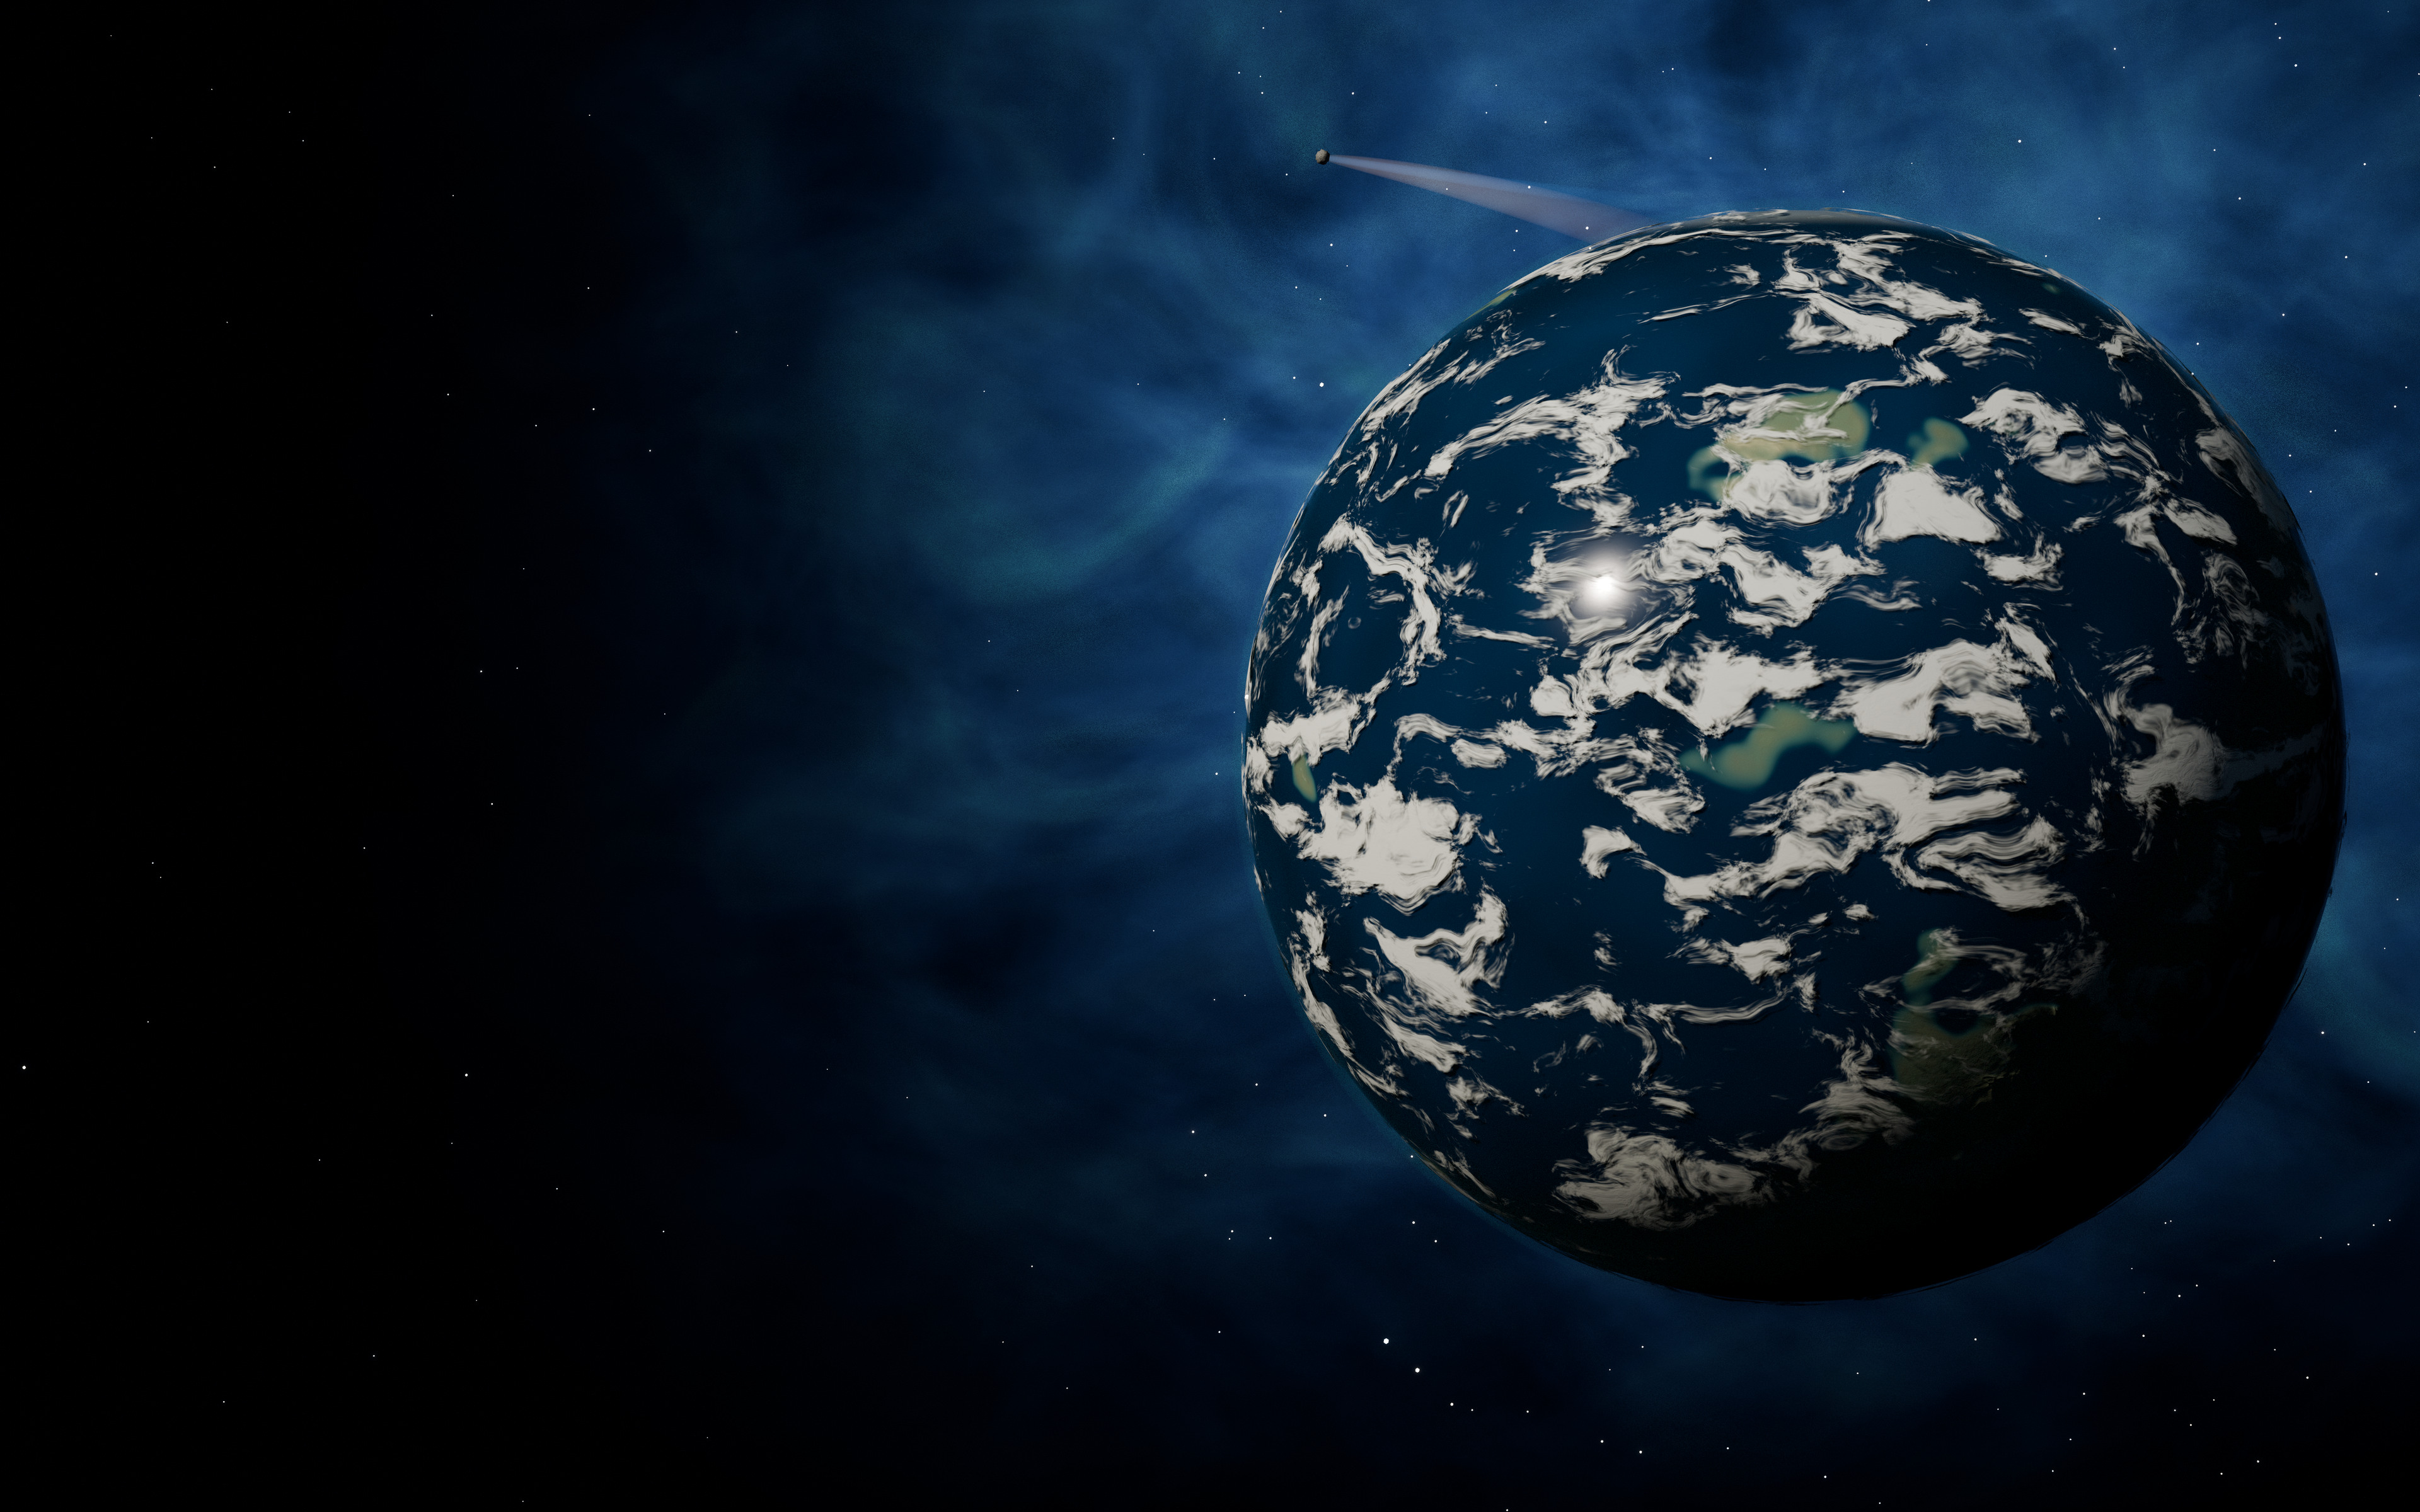
\includegraphics[width=\paperwidth,height=\paperheight]{Risorse/Copertine/M05_Pelago.jpg}};

\node[anchor=north west,inner sep=0,text width=9.2cm] at
 ([xshift=1.05cm,yshift=-1.10cm]current page.north west)
 {\color{Mint}\bfseries\fontsize{23}{27}\selectfont PELAGO};
\node[anchor=north west,inner sep=0,text width=9.2cm] at
 ([xshift=1.07cm,yshift=-2.16cm]current page.north west)
 {\color{white}\fontsize{9.0}{12}\selectfont MODULO M05 · SCIENZE DELLA TERRA};
\draw[Mint,line width=1.4pt] ([xshift=1.05cm,yshift=-2.78cm]current page.north west)--
 ([xshift=2.60cm,yshift=-2.78cm]current page.north west);
\node[anchor=north west,inner sep=0] at
 ([xshift=1.05cm,yshift=-3.35cm]current page.north west)
 {\begin{minipage}{9.2cm}\raggedright\color{white}\bfseries
 \fontsize{30}{36}\selectfont Campionamento,\\stima e\\incertezza\end{minipage}};
\node[anchor=north west,inner sep=0] at
 ([xshift=1.07cm,yshift=-7.88cm]current page.north west)
 {\begin{minipage}{9.0cm}\raggedright\color{Lilac}
 \fontsize{12.2}{17}\selectfont Disegni campionari, intervalli\\di confidenza e bootstrap\end{minipage}};
\node[anchor=north west,inner sep=0,text width=9.2cm] at
 ([xshift=1.07cm,yshift=-10.52cm]current page.north west)
 {\color{white}\fontsize{11.5}{15}\selectfont Marzio De Corato};
\node[anchor=north west,inner sep=0,text width=9.2cm] at
 ([xshift=1.07cm,yshift=-11.17cm]current page.north west)
 {\color{Lilac}\fontsize{8.8}{11}\selectfont \href{https://creativecommons.org/licenses/by-nc-sa/4.0/}{\textcopyright{} 2026 · CC BY-NC-SA 4.0}};
\end{tikzpicture}
\end{frame}


\begin{frame}[plain]\hypertarget{slide2}{}
\bookmark[level=0,page=2]{Domanda centrale}
\begin{tikzpicture}[remember picture,overlay]
\node[anchor=north west,inner sep=0] at ([xshift=.95cm,yshift=-.67cm]current page.north west) {\color{Navy}\bfseries\fontsize{23}{27}\selectfont Dal campione alla popolazione};
\draw[Classical,line width=1.4pt] ([xshift=.95cm,yshift=-1.73cm]current page.north west)--([xshift=2.5cm,yshift=-1.73cm]current page.north west);
\node[anchor=north west,inner sep=0,fill=GeoTint,rounded corners=2mm,text width=17.7cm,inner sep=3.5mm] at ([xshift=1.0cm,yshift=-2.26cm]current page.north west) {\color{Navy}\fontsize{14.1}{19}\selectfont Quando una stima può rappresentare unità che non abbiamo osservato?};
\node[draw=Rule,line width=.7pt,fill=GeoTint,rounded corners=2.5mm,minimum width=4.8cm,minimum height=2.15cm,text width=4.38cm,align=center,inner sep=3mm] (n0) at ([xshift=4cm,yshift=-6.15cm]current page.north west) {\color{Navy}\bfseries\fontsize{13}{16}\selectfont DISEGNO\\[2mm]\color{Ink}\normalfont\fontsize{10.5}{14}\selectfont Unità e selezione};
\node[draw=Rule,line width=.7pt,fill=Paper,rounded corners=2.5mm,minimum width=4.8cm,minimum height=2.15cm,text width=4.38cm,align=center,inner sep=3mm] (n1) at ([xshift=10cm,yshift=-6.15cm]current page.north west) {\color{Navy}\bfseries\fontsize{13}{16}\selectfont STIMA\\[2mm]\color{Ink}\normalfont\fontsize{10.5}{14}\selectfont Parametro e statistica};
\node[draw=Rule,line width=.7pt,fill=GeoTint,rounded corners=2.5mm,minimum width=4.8cm,minimum height=2.15cm,text width=4.38cm,align=center,inner sep=3mm] (n2) at ([xshift=16cm,yshift=-6.15cm]current page.north west) {\color{Navy}\bfseries\fontsize{13}{16}\selectfont INCERTEZZA\\[2mm]\color{Ink}\normalfont\fontsize{10.5}{14}\selectfont Errore standard\\e copertura};
\draw[-{Stealth[length=3.0mm]},draw=Classical,line width=1.45pt] ([xshift=6.65cm,yshift=-6.15cm]current page.north west)--([xshift=7.35cm,yshift=-6.15cm]current page.north west);
\draw[-{Stealth[length=3.0mm]},draw=Classical,line width=1.45pt] ([xshift=12.65cm,yshift=-6.15cm]current page.north west)--([xshift=13.35cm,yshift=-6.15cm]current page.north west);
\node[anchor=north west,inner sep=0,text width=17.9cm] at ([xshift=1.05cm,yshift=-8.25cm]current page.north west) {\color{Classical}\bfseries\fontsize{10.4}{13.4}\selectfont IDEA GUIDA};
\node[anchor=north west,inner sep=0,text width=17.85cm] at ([xshift=1.05cm,yshift=-8.71cm]current page.north west) {\color{Ink}\fontsize{11.9}{16.0}\selectfont Una stima e il suo intervallo sono interpretabili solo rispetto all’estimando, alla selezione e alla dipendenza fra unità.};
\draw[Rule,line width=.35pt] ([xshift=.95cm,yshift=-11.92cm]current page.north west)--([xshift=19.05cm,yshift=-11.92cm]current page.north west);
\node[anchor=north west,inner sep=0] at ([xshift=.95cm,yshift=-12.06cm]current page.north west) {\color{Muted}\fontsize{7.7}{9.3}\selectfont Pelago · Campionamento, stima e incertezza};
\node[anchor=north east,inner sep=0] at ([xshift=19.05cm,yshift=-12.06cm]current page.north west) {\color{Muted}\fontsize{7.7}{9.3}\selectfont 2/109};
\end{tikzpicture}
\end{frame}
\begin{frame}[plain]\hypertarget{slide3}{}
\bookmark[level=1,page=3]{Dal modello ai campioni possibili}
\begin{tikzpicture}[remember picture,overlay]
\PilotChrome{Dal modello ai campioni possibili}{POPOLAZIONI E PARAMETRI}{3}{Una stima dipende sia dai valori osservati sia dal modo in cui il campione è stato raccolto.}
\node[anchor=north west,inner sep=0] at ([xshift=0.96cm,yshift=-2.13cm]current page.north west) {\usebox{\PilotLeftBox}};
\node[anchor=north west,inner sep=0] at ([xshift=11.52cm,yshift=-2.13cm]current page.north west) {\usebox{\PilotRightBox}};

\end{tikzpicture}\end{frame}

% SLIDE 004 | Popolazione, lista di selezione e campione
\begin{lrbox}{\PilotLeftBox}%
\begin{minipage}[t]{10.05cm}\raggedright\color{Ink}\fontsize{11.3}{14.8}\selectfont

\PLabel{Tre insiemi da distinguere}
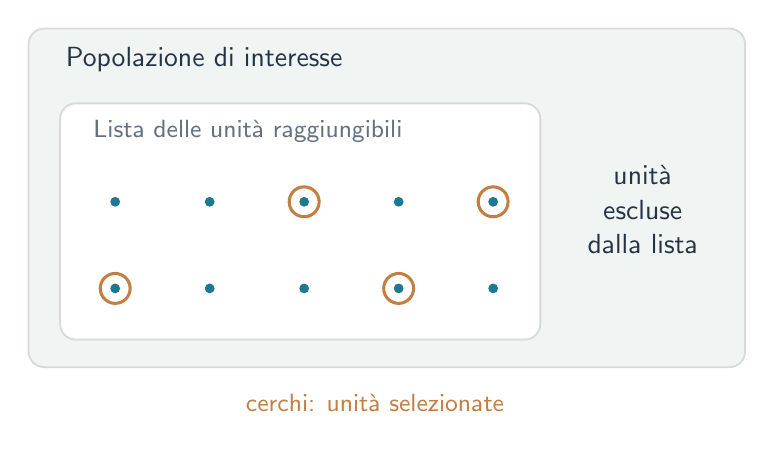
\begin{tikzpicture}[x=1cm,y=1cm]
\draw[pGroup,fill=GeoTint](.2,.1) rectangle(9.3,4.4);
\node[pLabel,anchor=west] at(.55,4){Popolazione di interesse};
\draw[pGroup](.6,.45) rectangle(6.7,3.45);
\node[pNote,anchor=west] at(.9,3.1){Lista delle unità raggiungibili};
\foreach \x/\y in {1.3/1.1,2.5/1.1,3.7/1.1,4.9/1.1,6.1/1.1,1.3/2.2,2.5/2.2,3.7/2.2,4.9/2.2,6.1/2.2}
\node[pDotA] at(\x,\y){};
\foreach \x/\y in {1.3/1.1,3.7/2.2,4.9/1.1,6.1/2.2}
\draw[GeoB,line width=1.1pt](\x,\y) circle(.19);
\node[pLabel,text width=1.8cm] at(8,2.1){unità\\escluse\\dalla lista};
\node[pNote,text=GeoB] at(4.6,-.35){cerchi: unità selezionate};
\end{tikzpicture}
\PSmall{Schema di appartenenza. Le unità escluse dalla lista restano senza osservazioni anche quando il prelievo dalla lista è casuale.}

\end{minipage}% 
\end{lrbox}
\typeout{FULLBOX:004:L:\the\ht\PilotLeftBox:\the\dp\PilotLeftBox}
\begin{lrbox}{\PilotRightBox}%
\begin{minipage}[t]{7.55cm}\raggedright\color{Ink}\fontsize{11.3}{14.8}\selectfont

\PCode{R · selezione da una lista completa}{004_popolazione.R}
\PSmall{Qui conosciamo tutta la popolazione finita. In una ricerca reale la lista può contenere gli identificativi senza riportare ancora i valori della variabile.}
\PInfo{Prima del prelievo: area, periodo, tipo di unità, criteri di inclusione e lista da cui si seleziona.}

\end{minipage}% 
\end{lrbox}
\typeout{FULLBOX:004:R:\the\ht\PilotRightBox:\the\dp\PilotRightBox}
\begin{frame}[plain]\hypertarget{slide4}{}
\bookmark[level=1,page=4]{Popolazione, lista di selezione e campione}
\begin{tikzpicture}[remember picture,overlay]
\PilotChrome{Popolazione, lista di selezione e campione}{POPOLAZIONI E PARAMETRI}{4}{La popolazione di interesse e l’insieme delle unità effettivamente selezionabili possono essere diversi.}
\node[anchor=north west,inner sep=0] at ([xshift=0.96cm,yshift=-2.13cm]current page.north west) {\usebox{\PilotLeftBox}};
\node[anchor=north west,inner sep=0] at ([xshift=11.52cm,yshift=-2.13cm]current page.north west) {\usebox{\PilotRightBox}};

\end{tikzpicture}\end{frame}

% SLIDE 005 | Una stazione può fornire più osservazioni
\begin{lrbox}{\PilotLeftBox}%
\begin{minipage}[t]{10.05cm}\raggedright\color{Ink}\fontsize{11.3}{14.8}\selectfont

\PLabel{Il livello del prelievo}
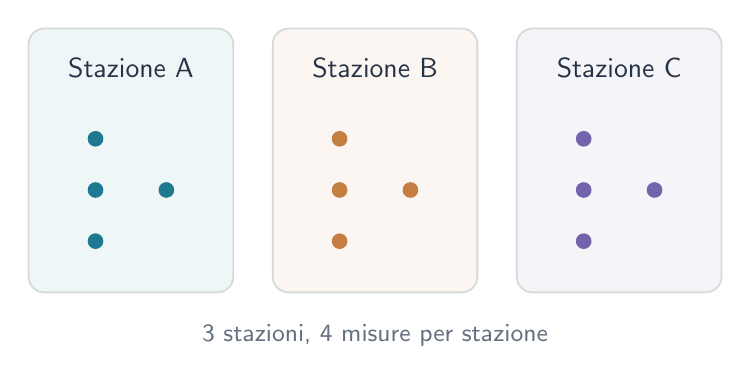
\begin{tikzpicture}[x=1cm,y=1cm]
\foreach \xx/\lab/\col in {1.6/A/GeoA,4.7/B/GeoB,7.8/C/GeoC}{
\draw[pGroup,fill=\col!7](\xx-1.3,.35) rectangle(\xx+1.3,3.7);
\node[pLabel] at(\xx,3.2){Stazione \lab};
\foreach \yy in {1,1.65,2.3}\node[circle,fill=\col,inner sep=2pt] at(\xx-.45,\yy){};
\node[circle,fill=\col,inner sep=2pt] at(\xx+.45,1.65){};
}
\node[pNote] at(4.7,-.2){3 stazioni, 4 misure per stazione};
\end{tikzpicture}
\PBody{Vicinanza e storia comune possono rendere simili le misure della stessa stazione. Il numero di righe descrive solo una parte del disegno.}

\end{minipage}% 
\end{lrbox}
\typeout{FULLBOX:005:L:\the\ht\PilotLeftBox:\the\dp\PilotLeftBox}
\begin{lrbox}{\PilotRightBox}%
\begin{minipage}[t]{7.55cm}\raggedright\color{Ink}\fontsize{11.3}{14.8}\selectfont

\PCode{R · righe e unità di prelievo}{005_unita.R}
\PSmall{Valori costruiti per l'esempio.}
\PInfo{$G$: numero di stazioni.\\$n_g$: misure nella stazione $g$.\\$n=\sum_g n_g$: osservazioni totali.}

\end{minipage}% 
\end{lrbox}
\typeout{FULLBOX:005:R:\the\ht\PilotRightBox:\the\dp\PilotRightBox}
\begin{frame}[plain]\hypertarget{slide5}{}
\bookmark[level=1,page=5]{Una stazione può fornire più osservazioni}
\begin{tikzpicture}[remember picture,overlay]
\PilotChrome{Una stazione può fornire più osservazioni}{POPOLAZIONI E PARAMETRI}{5}{La dipendenza fra osservazioni richiede di conservare gli identificativi delle unità a cui appartengono.}
\node[anchor=north west,inner sep=0] at ([xshift=0.96cm,yshift=-2.13cm]current page.north west) {\usebox{\PilotLeftBox}};
\node[anchor=north west,inner sep=0] at ([xshift=11.52cm,yshift=-2.13cm]current page.north west) {\usebox{\PilotRightBox}};

\end{tikzpicture}\end{frame}

% SLIDE 006 | Parametro, stimatore e stima osservata
\begin{lrbox}{\PilotLeftBox}%
\begin{minipage}[t]{10.05cm}\raggedright\color{Ink}\fontsize{11.3}{14.8}\selectfont

\PLabel{Prima e dopo l'osservazione}
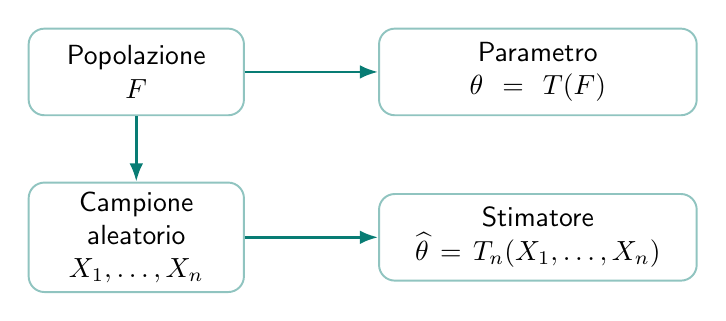
\begin{tikzpicture}[x=1cm,y=1cm]
\node[pFlow,text width=2.5cm] (f) at(1.7,3){Popolazione\\$F$};
\node[pFlow,text width=3.8cm] (th) at(6.8,3){Parametro\\$\theta=T(F)$};
\node[pFlow,text width=2.5cm] (x) at(1.7,.9){Campione aleatorio\\$X_1,\ldots,X_n$};
\node[pFlow,text width=3.8cm] (t) at(6.8,.9){Stimatore\\$\widehat\theta=T_n(X_1,\ldots,X_n)$};
\draw[pEdge](f)--(th);\draw[pEdge](f)--(x);\draw[pEdge](x)--(t);
\end{tikzpicture}
\[
X_i=x_i\quad\Longrightarrow\quad
\widehat\theta_{\mathrm{oss}}=T_n(x_1,\ldots,x_n).
\]
\PSmall{Il parametro resta fisso. Lo stimatore varia fra campioni. La stima osservata è il valore calcolato.}

\end{minipage}% 
\end{lrbox}
\typeout{FULLBOX:006:L:\the\ht\PilotLeftBox:\the\dp\PilotLeftBox}
\begin{lrbox}{\PilotRightBox}%
\begin{minipage}[t]{7.55cm}\raggedright\color{Ink}\fontsize{11.3}{14.8}\selectfont

\PCode{R · una regola e un risultato}{006_stimatore.R}
\PSmall{Qui $\mu=10$ è noto perché generiamo i dati. \texttt{x06} contiene un campione e produce una stima.}
\PInfo{Maiuscole per variabili aleatorie, minuscole per valori osservati. L'asterisco indicherà il ricampionamento bootstrap.}

\end{minipage}% 
\end{lrbox}
\typeout{FULLBOX:006:R:\the\ht\PilotRightBox:\the\dp\PilotRightBox}
\begin{frame}[plain]\hypertarget{slide6}{}
\bookmark[level=1,page=6]{Parametro, stimatore e stima osservata}
\begin{tikzpicture}[remember picture,overlay]
\PilotChrome{Parametro, stimatore e stima osservata}{POPOLAZIONI E PARAMETRI}{6}{Il parametro è il bersaglio, lo stimatore è la regola di calcolo e la stima è il risultato sul campione.}
\node[anchor=north west,inner sep=0] at ([xshift=0.96cm,yshift=-2.13cm]current page.north west) {\usebox{\PilotLeftBox}};
\node[anchor=north west,inner sep=0] at ([xshift=11.52cm,yshift=-2.13cm]current page.north west) {\usebox{\PilotRightBox}};

\end{tikzpicture}\end{frame}

% SLIDE 007 | La domanda determina il parametro
\begin{lrbox}{\PilotLeftBox}%
\begin{minipage}[t]{10.05cm}\raggedright\color{Ink}\fontsize{11.3}{14.8}\selectfont

\PLabel{Tre domande su una variabile quantitativa}
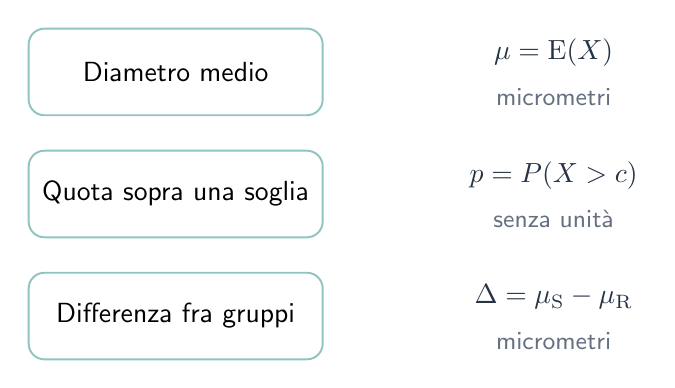
\begin{tikzpicture}[x=1cm,y=1cm]
\foreach \yy/\lab/\form/\unit in {
3.75/{Diametro medio}/{$\mu=\mathrm E(X)$}/{micrometri},
2.2/{Quota sopra una soglia}/{$p=P(X>c)$}/{senza unità},
.65/{Differenza fra gruppi}/{$\Delta=\mu_{\mathrm S}-\mu_{\mathrm R}$}/{micrometri}}{
\node[pFlow,text width=3.5cm] at(2,\yy){\lab};
\node[pLabel] at(6.8,\yy+.24){\form};
\node[pNote] at(6.8,\yy-.32){\unit};
}
\end{tikzpicture}
\PBody{La soglia $c$ e l'ordine del contrasto fanno parte della domanda. Un $\Delta$ positivo indica una media maggiore nel gruppo Spiky.}

\end{minipage}% 
\end{lrbox}
\typeout{FULLBOX:007:L:\the\ht\PilotLeftBox:\the\dp\PilotLeftBox}
\begin{lrbox}{\PilotRightBox}%
\begin{minipage}[t]{7.55cm}\raggedright\color{Ink}\fontsize{11.3}{14.8}\selectfont

\PCode{R · statistiche per tre domande}{007_bersagli.R}
\PSmall{La condizione \texttt{x07 > 6} produce valori logici. La loro media restituisce la proporzione osservata.}
\PInfo{Media e quota sopra soglia possono cambiare in modo diverso. La domanda guida la scelta della statistica.}

\end{minipage}% 
\end{lrbox}
\typeout{FULLBOX:007:R:\the\ht\PilotRightBox:\the\dp\PilotRightBox}
\begin{frame}[plain]\hypertarget{slide7}{}
\bookmark[level=1,page=7]{La domanda determina il parametro}
\begin{tikzpicture}[remember picture,overlay]
\PilotChrome{La domanda determina il parametro}{POPOLAZIONI E PARAMETRI}{7}{Prima del calcolo occorre precisare variabile, unità di misura, popolazione e parametro di interesse.}
\node[anchor=north west,inner sep=0] at ([xshift=0.96cm,yshift=-2.13cm]current page.north west) {\usebox{\PilotLeftBox}};
\node[anchor=north west,inner sep=0] at ([xshift=11.52cm,yshift=-2.13cm]current page.north west) {\usebox{\PilotRightBox}};

\end{tikzpicture}\end{frame}

% SLIDE 008 | I pesi definiscono quale media interessa
\begin{lrbox}{\PilotLeftBox}%
\begin{minipage}[t]{10.05cm}\raggedright\color{Ink}\fontsize{11.3}{14.8}\selectfont

\PLabel{Un parametro costruito su gruppi}
\[
\theta_w=\sum_{g=1}^{G}w_g\mu_g,\qquad
w_g\ge0,\quad\sum_gw_g=1.
\]
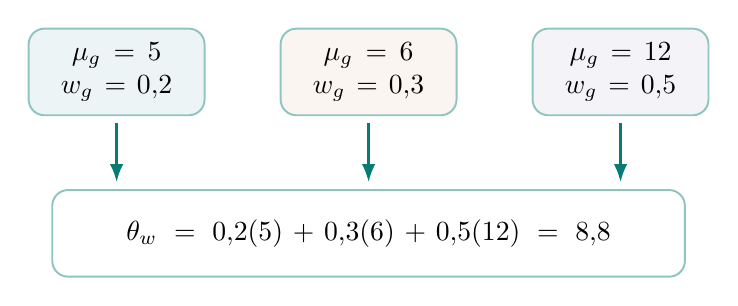
\begin{tikzpicture}[x=1cm,y=1cm]
\foreach \xx/\ww/\mm/\col in {1.5/{0{,}2}/5/GeoA,4.7/{0{,}3}/6/GeoB,7.9/{0{,}5}/12/GeoC}{
\node[pFlow,text width=2cm,fill=\col!8] at(\xx,2.3){$\mu_g=\mm$\\$w_g=\ww$};
\draw[pEdge](\xx,1.65)--(\xx,.9);
}
\node[pFlow,text width=7.8cm] at(4.7,.25){$\theta_w=0{,}2(5)+0{,}3(6)+0{,}5(12)=8{,}8$};
\end{tikzpicture}
\PSmall{I pesi possono descrivere quote note della popolazione o assegnare uguale importanza alle stazioni. Il criterio va dichiarato.}

\end{minipage}% 
\end{lrbox}
\typeout{FULLBOX:008:L:\the\ht\PilotLeftBox:\the\dp\PilotLeftBox}
\begin{lrbox}{\PilotRightBox}%
\begin{minipage}[t]{7.55cm}\raggedright\color{Ink}\fontsize{11.3}{14.8}\selectfont

\PCode{R · pesi normalizzati}{008_pesi.R}
\PSmall{\texttt{weighted.mean()} normalizza i pesi. Verificarne la somma rende trasparente il calcolo.}
\PInfo{La quota osservata nel campione e la quota nella popolazione coincidono soltanto in particolari disegni o realizzazioni.}

\end{minipage}% 
\end{lrbox}
\typeout{FULLBOX:008:R:\the\ht\PilotRightBox:\the\dp\PilotRightBox}
\begin{frame}[plain]\hypertarget{slide8}{}
\bookmark[level=1,page=8]{I pesi definiscono quale media interessa}
\begin{tikzpicture}[remember picture,overlay]
\PilotChrome{I pesi definiscono quale media interessa}{POPOLAZIONI E PARAMETRI}{8}{Cambiare i pesi può cambiare il parametro, anche mantenendo identici i valori delle medie di gruppo.}
\node[anchor=north west,inner sep=0] at ([xshift=0.96cm,yshift=-2.13cm]current page.north west) {\usebox{\PilotLeftBox}};
\node[anchor=north west,inner sep=0] at ([xshift=11.52cm,yshift=-2.13cm]current page.north west) {\usebox{\PilotRightBox}};

\end{tikzpicture}\end{frame}

% SLIDE 009 | Media delle misure e media delle stazioni
\begin{lrbox}{\PilotLeftBox}%
\begin{minipage}[t]{10.05cm}\raggedright\color{Ink}\fontsize{11.3}{14.8}\selectfont

\PLabel{Due stazioni con numerosità diverse}
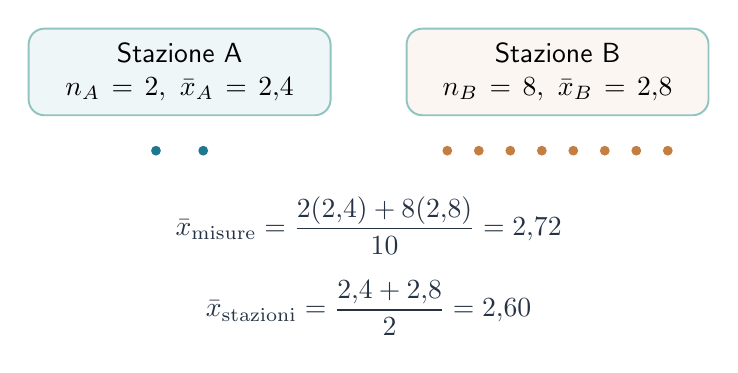
\begin{tikzpicture}[x=1cm,y=1cm]
\node[pFlow,text width=3.6cm,fill=GeoA!7] at(2.2,3.1){Stazione A\\$n_A=2,\ \bar x_A=2{,}4$};
\node[pFlow,text width=3.6cm,fill=GeoB!7] at(7,3.1){Stazione B\\$n_B=8,\ \bar x_B=2{,}8$};
\foreach \x in {1.9,2.5}\node[pDotA] at(\x,2.1){};
\foreach \x in {5.6,6,6.4,6.8,7.2,7.6,8,8.4}\node[pDotB] at(\x,2.1){};
\node[pLabel] at(4.6,1.15){$\displaystyle\bar x_{\mathrm{misure}}=\frac{2(2{,}4)+8(2{,}8)}{10}=2{,}72$};
\node[pLabel] at(4.6,.1){$\displaystyle\bar x_{\mathrm{stazioni}}=\frac{2{,}4+2{,}8}{2}=2{,}60$};
\end{tikzpicture}
\PSmall{Unità: $\mathrm{g/cm^3}$. La prima media dà più peso alla stazione con più misure. La seconda dà peso $1/2$ a ciascuna stazione.}

\end{minipage}% 
\end{lrbox}
\typeout{FULLBOX:009:L:\the\ht\PilotLeftBox:\the\dp\PilotLeftBox}
\begin{lrbox}{\PilotRightBox}%
\begin{minipage}[t]{7.55cm}\raggedright\color{Ink}\fontsize{11.3}{14.8}\selectfont

\PCode{R · stessi valori, pesi diversi}{009_due_medie.R}
\PBody{Una raccolta più intensa in B non dimostra che B rappresenti una quota maggiore del territorio. Occorre precisare la quantità da stimare.}
\PInfo{Le formule coincidono se i gruppi hanno uguale numerosità oppure uguale media.}

\end{minipage}% 
\end{lrbox}
\typeout{FULLBOX:009:R:\the\ht\PilotRightBox:\the\dp\PilotRightBox}
\begin{frame}[plain]\hypertarget{slide9}{}
\bookmark[level=1,page=9]{Media delle misure e media delle stazioni}
\begin{tikzpicture}[remember picture,overlay]
\PilotChrome{Media delle misure e media delle stazioni}{POPOLAZIONI E PARAMETRI}{9}{La scelta fra media delle misure e media delle stazioni richiede una motivazione legata alla popolazione di interesse.}
\node[anchor=north west,inner sep=0] at ([xshift=0.96cm,yshift=-2.13cm]current page.north west) {\usebox{\PilotLeftBox}};
\node[anchor=north west,inner sep=0] at ([xshift=11.52cm,yshift=-2.13cm]current page.north west) {\usebox{\PilotRightBox}};

\end{tikzpicture}\end{frame}

% SLIDE 010 | Un disegno bilanciato rende uguali le due medie
\begin{lrbox}{\PilotLeftBox}%
\begin{minipage}[t]{10.05cm}\raggedright\color{Ink}\fontsize{11.3}{14.8}\selectfont

\PLabel{$n_g=m$ per tutte le $G$ stazioni}
\[
\bar x=\frac{1}{Gm}\sum_{g=1}^{G}\sum_{i=1}^{m}x_{gi}
=\frac1G\sum_{g=1}^{G}\bar x_g.
\]
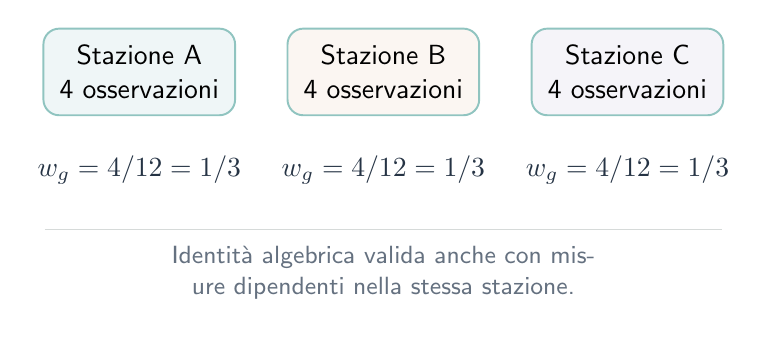
\begin{tikzpicture}[x=1cm,y=1cm]
\foreach \xx/\lab/\col in {1.6/A/GeoA,4.7/B/GeoB,7.8/C/GeoC}{
\node[pFlow,text width=2.2cm,fill=\col!7] at(\xx,2.1){Stazione \lab\\4 osservazioni};
\node[pLabel] at(\xx,.85){$w_g=4/12=1/3$};
}
\draw[Rule](.4,.1)--(9,.1);
\node[pNote,text width=8.8cm] at(4.7,-.45){Identità algebrica valida anche con misure dipendenti nella stessa stazione.};
\end{tikzpicture}
\PSmall{Il calcolo dell'errore standard richiede anche la struttura della dipendenza.}

\end{minipage}% 
\end{lrbox}
\typeout{FULLBOX:010:L:\the\ht\PilotLeftBox:\the\dp\PilotLeftBox}
\begin{lrbox}{\PilotRightBox}%
\begin{minipage}[t]{7.55cm}\raggedright\color{Ink}\fontsize{11.3}{14.8}\selectfont

\PCode{R · un'uguaglianza da verificare}{010_bilanciato.R}
\PSmall{\texttt{tapply()} suddivide la variabile in gruppi e applica la funzione indicata. Qui restituisce una media per stazione.}
\PInfo{Stessa stima puntuale e stesso numero di righe non garantiscono la stessa quantità di informazione.}

\end{minipage}% 
\end{lrbox}
\typeout{FULLBOX:010:R:\the\ht\PilotRightBox:\the\dp\PilotRightBox}
\begin{frame}[plain]\hypertarget{slide10}{}
\bookmark[level=1,page=10]{Un disegno bilanciato rende uguali le due medie}
\begin{tikzpicture}[remember picture,overlay]
\PilotChrome{Un disegno bilanciato rende uguali le due medie}{POPOLAZIONI E PARAMETRI}{10}{La coincidenza delle medie in un disegno bilanciato non risolve la questione dell’incertezza della stima.}
\node[anchor=north west,inner sep=0] at ([xshift=0.96cm,yshift=-2.13cm]current page.north west) {\usebox{\PilotLeftBox}};
\node[anchor=north west,inner sep=0] at ([xshift=11.52cm,yshift=-2.13cm]current page.north west) {\usebox{\PilotRightBox}};

\end{tikzpicture}\end{frame}

% SLIDE 011 | Media dei rapporti e rapporto dei totali
\begin{lrbox}{\PilotLeftBox}%
\begin{minipage}[t]{10.05cm}\raggedright\color{Ink}\fontsize{11.3}{14.8}\selectfont

\PLabel{Domanda e supporto fisico}
\[
\rho_i=\frac{m_i}{V_i},\qquad\bar\rho=\frac1n\sum_i\rho_i.
\]
\[
\rho_{\mathrm{tot}}=\frac{\sum_i m_i}{\sum_i V_i}
=\sum_i\frac{V_i}{\sum_jV_j}\rho_i.
\]
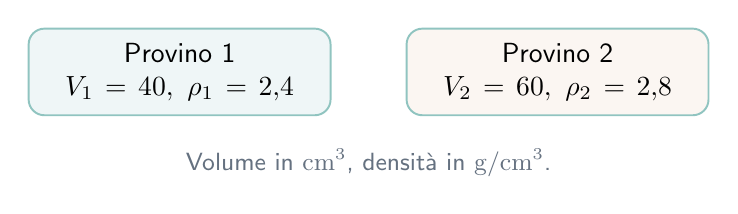
\begin{tikzpicture}[x=1cm,y=1cm]
\node[pFlow,text width=3.6cm,fill=GeoA!7] at(2.2,1.4){Provino 1\\$V_1=40,\ \rho_1=2{,}4$};
\node[pFlow,text width=3.6cm,fill=GeoB!7] at(7,1.4){Provino 2\\$V_2=60,\ \rho_2=2{,}8$};
\node[pNote] at(4.6,.25){Volume in $\mathrm{cm^3}$, densità in $\mathrm{g/cm^3}$.};
\end{tikzpicture}
\PSmall{Il rapporto dei totali pesa ciascuna densità con il volume del provino.}

\end{minipage}% 
\end{lrbox}
\typeout{FULLBOX:011:L:\the\ht\PilotLeftBox:\the\dp\PilotLeftBox}
\begin{lrbox}{\PilotRightBox}%
\begin{minipage}[t]{7.55cm}\raggedright\color{Ink}\fontsize{11.3}{14.8}\selectfont

\PCode{R · due quantità fisiche}{011_densita.R}
\PSmall{La media dei rapporti descrive il provino medio con pesi uguali. Il rapporto dei totali descrive massa complessiva per volume complessivo.}
\PInfo{La relazione deve indicare sia la formula usata per ogni osservazione sia il criterio di aggregazione.}

\end{minipage}% 
\end{lrbox}
\typeout{FULLBOX:011:R:\the\ht\PilotRightBox:\the\dp\PilotRightBox}
\begin{frame}[plain]\hypertarget{slide11}{}
\bookmark[level=1,page=11]{Media dei rapporti e rapporto dei totali}
\begin{tikzpicture}[remember picture,overlay]
\PilotChrome{Media dei rapporti e rapporto dei totali}{POPOLAZIONI E PARAMETRI}{11}{Aggregare prima o dopo una divisione può cambiare il parametro di interesse.}
\node[anchor=north west,inner sep=0] at ([xshift=0.96cm,yshift=-2.13cm]current page.north west) {\usebox{\PilotLeftBox}};
\node[anchor=north west,inner sep=0] at ([xshift=11.52cm,yshift=-2.13cm]current page.north west) {\usebox{\PilotRightBox}};

\end{tikzpicture}\end{frame}

% SLIDE 012 | Il campionamento casuale semplice
\begin{lrbox}{\PilotLeftBox}%
\begin{minipage}[t]{10.05cm}\raggedright\color{Ink}\fontsize{11.3}{14.8}\selectfont

\PLabel{Popolazione finita, senza reinserimento}
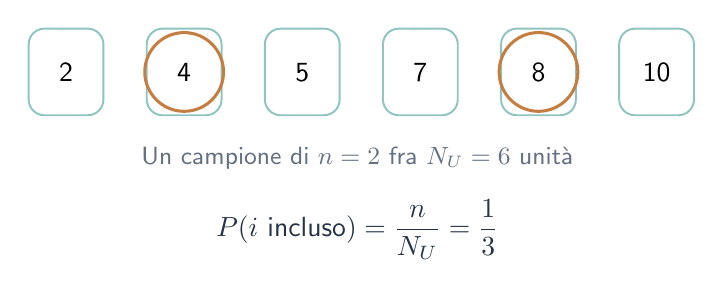
\begin{tikzpicture}[x=1cm,y=1cm]
\foreach \xx/\lab in {1/2,2.5/4,4/5,5.5/7,7/8,8.5/10}
\node[pFlow,minimum width=.95cm] at(\xx,2.6){\lab};
\draw[GeoB,line width=1.1pt](2.5,2.6) circle(.5);
\draw[GeoB,line width=1.1pt](7,2.6) circle(.5);
\node[pNote] at(4.7,1.5){Un campione di $n=2$ fra $N_U=6$ unità};
\node[pLabel] at(4.7,.6){$\displaystyle P(i\text{ incluso})=\frac{n}{N_U}=\frac13$};
\end{tikzpicture}
\[
\mathrm E_d(\bar X)=\bar Y_U,\qquad
\bar Y_U=\frac1{N_U}\sum_{i\in U}y_i.
\]
\PSmall{$\mathrm E_d$ media sui campioni del disegno. Ogni sottoinsieme di due unità ha uguale probabilità.}

\end{minipage}% 
\end{lrbox}
\typeout{FULLBOX:012:L:\the\ht\PilotLeftBox:\the\dp\PilotLeftBox}
\begin{lrbox}{\PilotRightBox}%
\begin{minipage}[t]{7.55cm}\raggedright\color{Ink}\fontsize{11.3}{14.8}\selectfont

\PCode{R · enumerare i campioni}{012_casuale_semplice.R}
\PSmall{\texttt{combn()} elenca le 15 coppie. La media delle loro medie coincide con quella della popolazione.}
\PInfo{La casualità deve riguardare la selezione. Mescolare le righe dopo una raccolta selettiva lascia invariato il campione.}

\end{minipage}% 
\end{lrbox}
\typeout{FULLBOX:012:R:\the\ht\PilotRightBox:\the\dp\PilotRightBox}
\begin{frame}[plain]\hypertarget{slide12}{}
\bookmark[level=1,page=12]{Il campionamento casuale semplice}
\begin{tikzpicture}[remember picture,overlay]
\PilotChrome{Il campionamento casuale semplice}{POPOLAZIONI E PARAMETRI}{12}{La non distorsione della media nel campionamento casuale semplice deriva dalle probabilità del disegno.}
\node[anchor=north west,inner sep=0] at ([xshift=0.96cm,yshift=-2.13cm]current page.north west) {\usebox{\PilotLeftBox}};
\node[anchor=north west,inner sep=0] at ([xshift=11.52cm,yshift=-2.13cm]current page.north west) {\usebox{\PilotRightBox}};

\end{tikzpicture}\end{frame}

% SLIDE 013 | La stima stratificata usa le quote della popolazione
\begin{lrbox}{\PilotLeftBox}%
\begin{minipage}[t]{10.05cm}\raggedright\color{Ink}\fontsize{11.3}{14.8}\selectfont

\PLabel{Strati definiti prima della selezione}
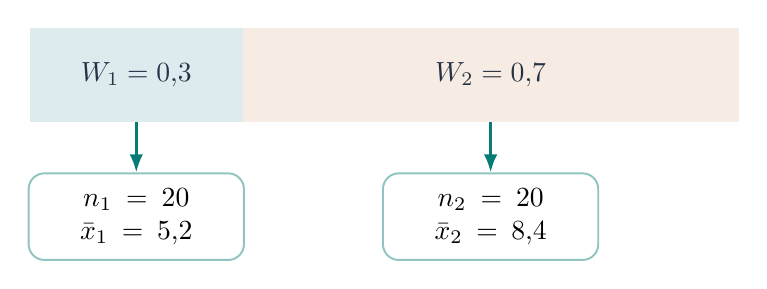
\begin{tikzpicture}[x=1cm,y=1cm]
\fill[GeoA!15](.3,2.1) rectangle(3,3.3);
\fill[GeoB!15](3,2.1) rectangle(9.3,3.3);
\node[pLabel] at(1.65,2.7){$W_1=0{,}3$};
\node[pLabel] at(6.15,2.7){$W_2=0{,}7$};
\node[pFlow,text width=2.5cm] (a) at(1.65,.9){$n_1=20$\\$\bar x_1=5{,}2$};
\node[pFlow,text width=2.5cm] (b) at(6.15,.9){$n_2=20$\\$\bar x_2=8{,}4$};
\draw[pEdge](1.65,2.1)--(a);\draw[pEdge](6.15,2.1)--(b);
\end{tikzpicture}
\[
\widehat\theta_{\mathrm{str}}=\sum_{h=1}^{H}W_h\bar X_h,
\qquad W_h=\frac{N_h}{N_U}.
\]
\PSmall{Il prelievo casuale avviene separatamente in ogni strato. Le quote $W_h$ si riferiscono alla popolazione.}

\end{minipage}% 
\end{lrbox}
\typeout{FULLBOX:013:L:\the\ht\PilotLeftBox:\the\dp\PilotLeftBox}
\begin{lrbox}{\PilotRightBox}%
\begin{minipage}[t]{7.55cm}\raggedright\color{Ink}\fontsize{11.3}{14.8}\selectfont

\PCode{R · quote note e quote raccolte}{013_strati.R}
\PBody{Campione: metà osservazioni per strato. Popolazione: quote $30\%$ e $70\%$. I pesi seguono il parametro.}
\PInfo{La fonte dei pesi deve essere esplicita: dimensione degli strati, area rappresentata o altro criterio pertinente.}

\end{minipage}% 
\end{lrbox}
\typeout{FULLBOX:013:R:\the\ht\PilotRightBox:\the\dp\PilotRightBox}
\begin{frame}[plain]\hypertarget{slide13}{}
\bookmark[level=1,page=13]{La stima stratificata usa le quote della popolazione}
\begin{tikzpicture}[remember picture,overlay]
\PilotChrome{La stima stratificata usa le quote della popolazione}{POPOLAZIONI E PARAMETRI}{13}{L’allocazione del campione fra strati può differire dalla loro importanza nella popolazione.}
\node[anchor=north west,inner sep=0] at ([xshift=0.96cm,yshift=-2.13cm]current page.north west) {\usebox{\PilotLeftBox}};
\node[anchor=north west,inner sep=0] at ([xshift=11.52cm,yshift=-2.13cm]current page.north west) {\usebox{\PilotRightBox}};

\end{tikzpicture}\end{frame}

% SLIDE 014 | Selezionare stazioni e poi misure
\begin{lrbox}{\PilotLeftBox}%
\begin{minipage}[t]{10.05cm}\raggedright\color{Ink}\fontsize{11.3}{14.8}\selectfont

\PLabel{Un disegno con unità raggruppate}
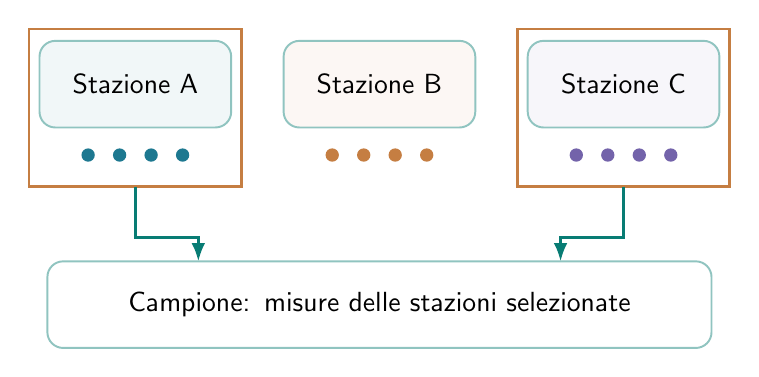
\begin{tikzpicture}[x=1cm,y=1cm]
\foreach \xx/\lab/\col in {1.6/A/GeoA,4.7/B/GeoB,7.8/C/GeoC}{
\node[pFlow,text width=2.2cm,fill=\col!6] at(\xx,3.5){Stazione \lab};
\foreach \dx in {-.6,-.2,.2,.6}\node[circle,fill=\col,inner sep=1.7pt] at(\xx+\dx,2.6){};
}
\draw[GeoB,line width=1pt](.25,2.2) rectangle(2.95,4.2);
\draw[GeoB,line width=1pt](6.45,2.2) rectangle(9.15,4.2);
\node[pFlow,text width=8.2cm] at(4.7,.7){Campione: misure delle stazioni selezionate};
\draw[pEdge](1.6,2.2)--(1.6,1.55)--(2.4,1.55)--(2.4,1.25);
\draw[pEdge](7.8,2.2)--(7.8,1.55)--(7,1.55)--(7,1.25);
\end{tikzpicture}
\PSmall{Schema esemplificativo. Si possono osservare tutte le misure disponibili o selezionare ulteriori unità a un secondo stadio.}

\end{minipage}% 
\end{lrbox}
\typeout{FULLBOX:014:L:\the\ht\PilotLeftBox:\the\dp\PilotLeftBox}
\begin{lrbox}{\PilotRightBox}%
\begin{minipage}[t]{7.55cm}\raggedright\color{Ink}\fontsize{11.3}{14.8}\selectfont

\PCode{R · una selezione gerarchica}{014_selezione_stazioni.R}
\PSmall{\texttt{\%in\%} riconosce le righe delle stazioni scelte. L'appartenenza resta conservata nella tabella.}
\PInfo{Il bootstrap per stazioni riprenderà questo livello di organizzazione delle osservazioni.}

\end{minipage}% 
\end{lrbox}
\typeout{FULLBOX:014:R:\the\ht\PilotRightBox:\the\dp\PilotRightBox}
\begin{frame}[plain]\hypertarget{slide14}{}
\bookmark[level=1,page=14]{Selezionare stazioni e poi misure}
\begin{tikzpicture}[remember picture,overlay]
\PilotChrome{Selezionare stazioni e poi misure}{POPOLAZIONI E PARAMETRI}{14}{Il livello della selezione orienta il calcolo dell’incertezza e il successivo ricampionamento.}
\node[anchor=north west,inner sep=0] at ([xshift=0.96cm,yshift=-2.13cm]current page.north west) {\usebox{\PilotLeftBox}};
\node[anchor=north west,inner sep=0] at ([xshift=11.52cm,yshift=-2.13cm]current page.north west) {\usebox{\PilotRightBox}};

\end{tikzpicture}\end{frame}

% SLIDE 015 | Laboratorio: quanto pesa la stazione C?
\begin{lrbox}{\PilotLeftBox}%
\begin{minipage}[t]{10.05cm}\raggedright\color{Ink}\fontsize{11.3}{14.8}\selectfont

\PLab{https://marzione00.github.io/Lab_Geo/\#laboratorio/m05-estimandi}{Esperimento · misure o stazioni}
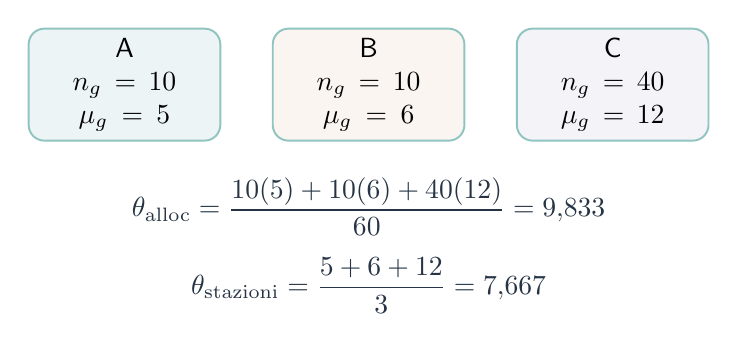
\begin{tikzpicture}[x=1cm,y=1cm]
\foreach \xx/\lab/\ng/\mg/\col in {1.6/A/10/5/GeoA,4.7/B/10/6/GeoB,7.8/C/40/12/GeoC}{
\node[pFlow,text width=2.2cm,fill=\col!8] at(\xx,2.9){\lab\\$n_g=\ng$\\$\mu_g=\mg$};
}
\node[pLabel] at(4.7,1.35){$\displaystyle\theta_{\mathrm{alloc}}=\frac{10(5)+10(6)+40(12)}{60}=9{,}833$};
\node[pLabel] at(4.7,.35){$\displaystyle\theta_{\mathrm{stazioni}}=\frac{5+6+12}{3}=7{,}667$};
\end{tikzpicture}
\PSmall{Osservazioni normali con deviazione standard 1. Le formule riportano i bersagli teorici. Le medie osservate oscillano.}

\end{minipage}% 
\end{lrbox}
\typeout{FULLBOX:015:L:\the\ht\PilotLeftBox:\the\dp\PilotLeftBox}
\begin{lrbox}{\PilotRightBox}%
\begin{minipage}[t]{7.55cm}\raggedright\color{Ink}\fontsize{11.3}{14.8}\selectfont

\PCode{R · due allocazioni}{015_lab_estimandi.R}
\PBody{Confrontare \texttt{nHigh = 10} e \texttt{nHigh = 40}. Annotare pesi e risultati delle due medie.}
\PInfo{Aumentando \texttt{nHigh} cambiano sia il peso sia le osservazioni generate per C. Anche la sua media osservata può cambiare.}

\end{minipage}% 
\end{lrbox}
\typeout{FULLBOX:015:R:\the\ht\PilotRightBox:\the\dp\PilotRightBox}
\begin{frame}[plain]\hypertarget{slide15}{}
\bookmark[level=1,page=15]{Laboratorio: quanto pesa la stazione C?}
\begin{tikzpicture}[remember picture,overlay]
\PilotChrome{Laboratorio: quanto pesa la stazione C?}{POPOLAZIONI E PARAMETRI}{15}{Il confronto richiede di separare la variazione dei pesi dalla variazione casuale delle medie osservate.}
\node[anchor=north west,inner sep=0] at ([xshift=0.96cm,yshift=-2.13cm]current page.north west) {\usebox{\PilotLeftBox}};
\node[anchor=north west,inner sep=0] at ([xshift=11.52cm,yshift=-2.13cm]current page.north west) {\usebox{\PilotRightBox}};

\end{tikzpicture}\end{frame}

% SLIDE 016 | L’accessibilità può modificare il campione
\begin{lrbox}{\PilotLeftBox}%
\begin{minipage}[t]{10.05cm}\raggedright\color{Ink}\fontsize{11.3}{14.8}\selectfont

\PLabel{Copertura incompleta: esempio costruito}
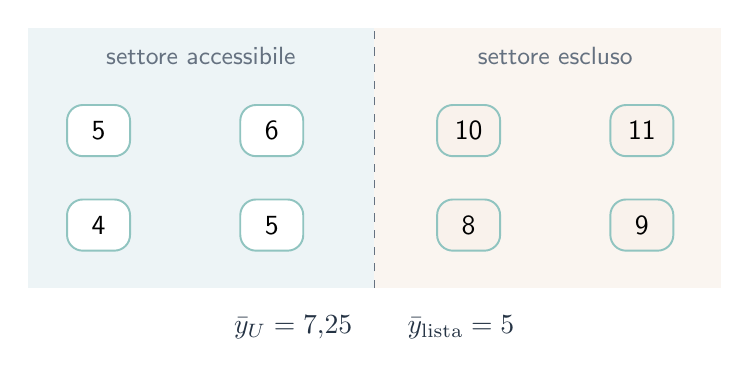
\begin{tikzpicture}[x=1cm,y=1cm]
\fill[GeoA!8](.3,.4) rectangle(4.7,3.7);
\fill[GeoB!8](4.7,.4) rectangle(9.1,3.7);
\draw[Muted,dashed](4.7,.4)--(4.7,3.7);
\foreach \x/\y/\v in {1.2/1.2/4,3.4/1.2/5,1.2/2.4/5,3.4/2.4/6}
\node[pFlow,minimum width=.8cm,minimum height=.65cm] at(\x,\y){\v};
\foreach \x/\y/\v in {5.9/1.2/8,8.1/1.2/9,5.9/2.4/10,8.1/2.4/11}
\node[pFlow,minimum width=.8cm,minimum height=.65cm,fill=GeoB!10] at(\x,\y){\v};
\node[pNote] at(2.5,3.35){settore accessibile};
\node[pNote] at(7,3.35){settore escluso};
\node[pLabel] at(4.7,-.1){$\bar y_U=7{,}25\qquad\bar y_{\mathrm{lista}}=5$};
\end{tikzpicture}
\PSmall{Se il settore escluso ha valori diversi, la media della lista può differire da quella della popolazione.}

\end{minipage}% 
\end{lrbox}
\typeout{FULLBOX:016:L:\the\ht\PilotLeftBox:\the\dp\PilotLeftBox}
\begin{lrbox}{\PilotRightBox}%
\begin{minipage}[t]{7.55cm}\raggedright\color{Ink}\fontsize{11.3}{14.8}\selectfont

\PCode{R · effetto di una lista parziale}{016_lista_incompleta.R}
\PBody{Più osservazioni nel settore accessibile possono stabilizzare la stima sulla popolazione incompleta.}
\PInfo{Per interpretare la selezione servono informazioni sulle unità escluse e sui motivi dell'esclusione.}

\end{minipage}% 
\end{lrbox}
\typeout{FULLBOX:016:R:\the\ht\PilotRightBox:\the\dp\PilotRightBox}
\begin{frame}[plain]\hypertarget{slide16}{}
\bookmark[level=1,page=16]{L’accessibilità può modificare il campione}
\begin{tikzpicture}[remember picture,overlay]
\PilotChrome{L’accessibilità può modificare il campione}{SELEZIONE E DISTORSIONE}{16}{La rappresentatività richiede un legame giustificabile fra le unità osservate e la popolazione a cui si estende il risultato.}
\node[anchor=north west,inner sep=0] at ([xshift=0.96cm,yshift=-2.13cm]current page.north west) {\usebox{\PilotLeftBox}};
\node[anchor=north west,inner sep=0] at ([xshift=11.52cm,yshift=-2.13cm]current page.north west) {\usebox{\PilotRightBox}};

\end{tikzpicture}\end{frame}

% SLIDE 017 | La distorsione è uno scarto medio
\begin{lrbox}{\PilotLeftBox}%
\begin{minipage}[t]{10.05cm}\raggedright\color{Ink}\fontsize{11.3}{14.8}\selectfont

\PLabel{Una proprietà delle ripetizioni}
\[
\operatorname{Bias}(\widehat\theta)=\mathrm E(\widehat\theta)-\theta.
\]
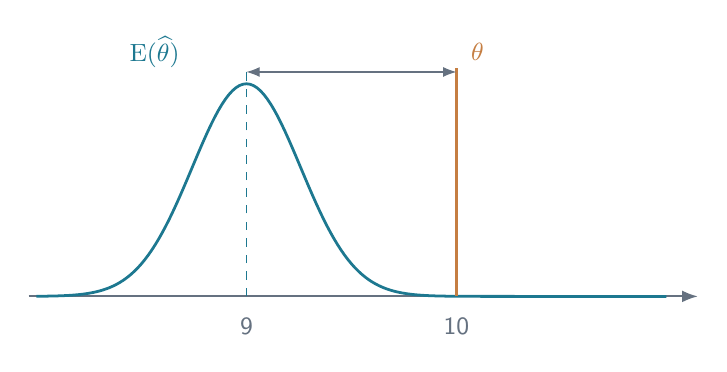
\begin{tikzpicture}[x=1cm,y=1cm]
\draw[pAxis](.5,.2)--(9,.2);
\draw[GeoA,line width=1pt] plot coordinates{(0.60000,0.20149) (0.64444,0.20191) (0.68889,0.20244) (0.73333,0.20310) (0.77778,0.20393) (0.82222,0.20495) (0.86667,0.20621) (0.91111,0.20776) (0.95556,0.20966) (1.00000,0.21197) (1.04444,0.21477) (1.08889,0.21815) (1.13333,0.22222) (1.17778,0.22708) (1.22222,0.23287) (1.26667,0.23974) (1.31111,0.24783) (1.35556,0.25734) (1.40000,0.26844) (1.44444,0.28136) (1.48889,0.29632) (1.53333,0.31355) (1.57778,0.33331) (1.62222,0.35585) (1.66667,0.38145) (1.71111,0.41038) (1.75556,0.44291) (1.80000,0.47929) (1.84444,0.51979) (1.88889,0.56464) (1.93333,0.61406) (1.97778,0.66821) (2.02222,0.72725) (2.06667,0.79126) (2.11111,0.86029) (2.15556,0.93430) (2.20000,1.01322) (2.24444,1.09688) (2.28889,1.18503) (2.33333,1.27735) (2.37778,1.37342) (2.42222,1.47274) (2.46667,1.57472) (2.51111,1.67871) (2.55556,1.78394) (2.60000,1.88962) (2.64444,1.99484) (2.68889,2.09870) (2.73333,2.20021) (2.77778,2.29839) (2.82222,2.39223) (2.86667,2.48074) (2.91111,2.56297) (2.95556,2.63798) (3.00000,2.70491) (3.04444,2.76297) (3.08889,2.81148) (3.13333,2.84985) (3.17778,2.87759) (3.22222,2.89438) (3.26667,2.90000) (3.31111,2.89438) (3.35556,2.87759) (3.40000,2.84985) (3.44444,2.81148) (3.48889,2.76297) (3.53333,2.70491) (3.57778,2.63798) (3.62222,2.56297) (3.66667,2.48074) (3.71111,2.39223) (3.75556,2.29839) (3.80000,2.20021) (3.84444,2.09870) (3.88889,1.99484) (3.93333,1.88962) (3.97778,1.78394) (4.02222,1.67871) (4.06667,1.57472) (4.11111,1.47274) (4.15556,1.37342) (4.20000,1.27735) (4.24444,1.18503) (4.28889,1.09688) (4.33333,1.01322) (4.37778,0.93430) (4.42222,0.86029) (4.46667,0.79126) (4.51111,0.72725) (4.55556,0.66821) (4.60000,0.61406) (4.64444,0.56464) (4.68889,0.51979) (4.73333,0.47929) (4.77778,0.44291) (4.82222,0.41038) (4.86667,0.38145) (4.91111,0.35585) (4.95556,0.33331) (5.00000,0.31355) (5.04444,0.29632) (5.08889,0.28136) (5.13333,0.26844) (5.17778,0.25734) (5.22222,0.24783) (5.26667,0.23974) (5.31111,0.23287) (5.35556,0.22708) (5.40000,0.22222) (5.44444,0.21815) (5.48889,0.21477) (5.53333,0.21197) (5.57778,0.20966) (5.62222,0.20776) (5.66667,0.20621) (5.71111,0.20495) (5.75556,0.20393) (5.80000,0.20310) (5.84444,0.20244) (5.88889,0.20191) (5.93333,0.20149) (5.97778,0.20116) (6.02222,0.20090) (6.06667,0.20069) (6.11111,0.20053) (6.15556,0.20041) (6.20000,0.20031) (6.24444,0.20023) (6.28889,0.20018) (6.33333,0.20013) (6.37778,0.20010) (6.42222,0.20007) (6.46667,0.20006) (6.51111,0.20004) (6.55556,0.20003) (6.60000,0.20002) (6.64444,0.20002) (6.68889,0.20001) (6.73333,0.20001) (6.77778,0.20001) (6.82222,0.20000) (6.86667,0.20000) (6.91111,0.20000) (6.95556,0.20000) (7.00000,0.20000) (7.04444,0.20000) (7.08889,0.20000) (7.13333,0.20000) (7.17778,0.20000) (7.22222,0.20000) (7.26667,0.20000) (7.31111,0.20000) (7.35556,0.20000) (7.40000,0.20000) (7.44444,0.20000) (7.48889,0.20000) (7.53333,0.20000) (7.57778,0.20000) (7.62222,0.20000) (7.66667,0.20000) (7.71111,0.20000) (7.75556,0.20000) (7.80000,0.20000) (7.84444,0.20000) (7.88889,0.20000) (7.93333,0.20000) (7.97778,0.20000) (8.02222,0.20000) (8.06667,0.20000) (8.11111,0.20000) (8.15556,0.20000) (8.20000,0.20000) (8.24444,0.20000) (8.28889,0.20000) (8.33333,0.20000) (8.37778,0.20000) (8.42222,0.20000) (8.46667,0.20000) (8.51111,0.20000) (8.55556,0.20000) (8.60000,0.20000)};
\draw[GeoA,dashed](3.2667,.2)--(3.2667,3.1);
\draw[GeoB,line width=.9pt](5.9333,.2)--(5.9333,3.1);
\node[pNote] at(3.2667,-.18){9};
\node[pNote] at(5.9333,-.18){10};
\node[pNote,text=GeoA] at(2.1,3.3){$\mathrm E(\widehat\theta)$};
\node[pNote,text=GeoB] at(6.2,3.3){$\theta$};
\draw[{Latex}-{Latex},Muted](3.2667,3.05)--(5.9333,3.05);
\end{tikzpicture}
\PSmall{Curva teorica: $\widehat\theta\sim N(9,4/60)$, bersaglio $\theta=10$. La distorsione vale $-1$.}

\end{minipage}% 
\end{lrbox}
\typeout{FULLBOX:017:L:\the\ht\PilotLeftBox:\the\dp\PilotLeftBox}
\begin{lrbox}{\PilotRightBox}%
\begin{minipage}[t]{7.55cm}\raggedright\color{Ink}\fontsize{11.3}{14.8}\selectfont

\PCode{R · media delle stime meno parametro}{017_bias.R}
\PSmall{La media di 200 stime approssima l'attesa. Il bias simulato può differire da $-1$ per errore Monte Carlo.}
\PInfo{L'errore di una singola stima è $\widehat\theta_{\mathrm{oss}}-\theta$. La distorsione media l'errore sulle ripetizioni.}

\end{minipage}% 
\end{lrbox}
\typeout{FULLBOX:017:R:\the\ht\PilotRightBox:\the\dp\PilotRightBox}
\begin{frame}[plain]\hypertarget{slide17}{}
\bookmark[level=1,page=17]{La distorsione è uno scarto medio}
\begin{tikzpicture}[remember picture,overlay]
\PilotChrome{La distorsione è uno scarto medio}{SELEZIONE E DISTORSIONE}{17}{Una singola osservazione dello scarto non permette di conoscere direttamente la distorsione dello stimatore.}
\node[anchor=north west,inner sep=0] at ([xshift=0.96cm,yshift=-2.13cm]current page.north west) {\usebox{\PilotLeftBox}};
\node[anchor=north west,inner sep=0] at ([xshift=11.52cm,yshift=-2.13cm]current page.north west) {\usebox{\PilotRightBox}};

\end{tikzpicture}\end{frame}

% SLIDE 018 | Errore quadratico: variabilità e distorsione
\begin{lrbox}{\PilotLeftBox}%
\begin{minipage}[t]{10.05cm}\raggedright\color{Ink}\fontsize{11.3}{14.8}\selectfont

\PLabel{La scomposizione della MSE}
\[
\begin{aligned}
\operatorname{MSE}(\widehat\theta)
&=\mathrm E[(\widehat\theta-\theta)^2]\\
&=\operatorname{Var}(\widehat\theta)
+\{\mathrm E(\widehat\theta)-\theta\}^{2}.
\end{aligned}
\]

\begin{tikzpicture}[x=1cm,y=1cm]
\node[pFlow,text width=3.4cm,fill=GeoA!8] at(2.1,1.8){Variabilità attorno\\alla propria attesa};
\node[pFlow,text width=3.4cm,fill=GeoB!8] at(7.1,1.8){Scarto dell'attesa\\dal parametro};
\node[pLabel] at(4.6,1.8){$+$};
\node[pNote,text width=8.8cm] at(4.6,.45){Il termine incrociato scompare perché\\$\mathrm E[\widehat\theta-\mathrm E(\widehat\theta)]=0$.};
\end{tikzpicture}
\PSmall{Varianza e MSE hanno l'unità del parametro al quadrato. La radice della MSE torna all'unità originale.}

\end{minipage}% 
\end{lrbox}
\typeout{FULLBOX:018:L:\the\ht\PilotLeftBox:\the\dp\PilotLeftBox}
\begin{lrbox}{\PilotRightBox}%
\begin{minipage}[t]{7.55cm}\raggedright\color{Ink}\fontsize{11.3}{14.8}\selectfont

\PCode{R · errore quadratico medio}{018_mse.R}
\PBody{La varianza è $4/60\simeq0{,}0667$. La distorsione al quadrato è $1$. La MSE vale circa $1{,}0667$.}
\PInfo{Una procedura molto concentrata può avere MSE elevata quando è concentrata lontano dal parametro.}

\end{minipage}% 
\end{lrbox}
\typeout{FULLBOX:018:R:\the\ht\PilotRightBox:\the\dp\PilotRightBox}
\begin{frame}[plain]\hypertarget{slide18}{}
\bookmark[level=1,page=18]{Errore quadratico: variabilità e distorsione}
\begin{tikzpicture}[remember picture,overlay]
\PilotChrome{Errore quadratico: variabilità e distorsione}{SELEZIONE E DISTORSIONE}{18}{La valutazione di una procedura considera sia la dispersione delle stime sia la loro distorsione.}
\node[anchor=north west,inner sep=0] at ([xshift=0.96cm,yshift=-2.13cm]current page.north west) {\usebox{\PilotLeftBox}};
\node[anchor=north west,inner sep=0] at ([xshift=11.52cm,yshift=-2.13cm]current page.north west) {\usebox{\PilotRightBox}};

\end{tikzpicture}\end{frame}

% SLIDE 019 | Più osservazioni riducono la varianza
\begin{lrbox}{\PilotLeftBox}%
\begin{minipage}[t]{10.05cm}\raggedright\color{Ink}\fontsize{11.3}{14.8}\selectfont

\PLabel{Il bias resta costante in questo modello}
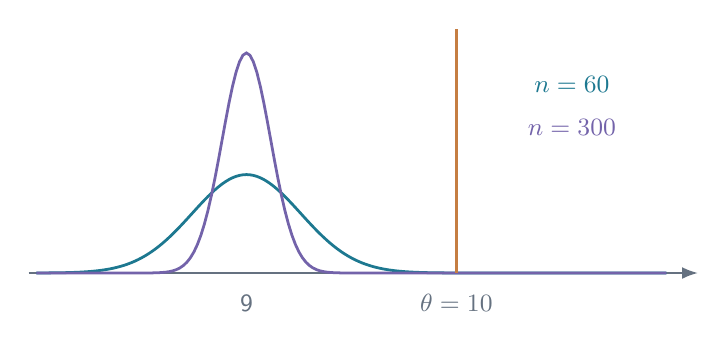
\begin{tikzpicture}[x=1cm,y=1cm]
\draw[pAxis](.5,.2)--(9,.2);
\draw[GeoA,line width=1pt] plot coordinates{(0.60000,0.20069) (0.64444,0.20089) (0.68889,0.20113) (0.73333,0.20144) (0.77778,0.20182) (0.82222,0.20229) (0.86667,0.20287) (0.91111,0.20359) (0.95556,0.20447) (1.00000,0.20554) (1.04444,0.20684) (1.08889,0.20840) (1.13333,0.21029) (1.17778,0.21254) (1.22222,0.21522) (1.26667,0.21840) (1.31111,0.22214) (1.35556,0.22654) (1.40000,0.23169) (1.44444,0.23767) (1.48889,0.24459) (1.53333,0.25257) (1.57778,0.26172) (1.62222,0.27215) (1.66667,0.28401) (1.71111,0.29740) (1.75556,0.31246) (1.80000,0.32930) (1.84444,0.34805) (1.88889,0.36882) (1.93333,0.39169) (1.97778,0.41677) (2.02222,0.44410) (2.06667,0.47373) (2.11111,0.50569) (2.15556,0.53996) (2.20000,0.57649) (2.24444,0.61522) (2.28889,0.65603) (2.33333,0.69877) (2.37778,0.74325) (2.42222,0.78923) (2.46667,0.83645) (2.51111,0.88459) (2.55556,0.93331) (2.60000,0.98223) (2.64444,1.03095) (2.68889,1.07903) (2.73333,1.12602) (2.77778,1.17147) (2.82222,1.21492) (2.86667,1.25590) (2.91111,1.29397) (2.95556,1.32869) (3.00000,1.35968) (3.04444,1.38656) (3.08889,1.40902) (3.13333,1.42678) (3.17778,1.43963) (3.22222,1.44740) (3.26667,1.45000) (3.31111,1.44740) (3.35556,1.43963) (3.40000,1.42678) (3.44444,1.40902) (3.48889,1.38656) (3.53333,1.35968) (3.57778,1.32869) (3.62222,1.29397) (3.66667,1.25590) (3.71111,1.21492) (3.75556,1.17147) (3.80000,1.12602) (3.84444,1.07903) (3.88889,1.03095) (3.93333,0.98223) (3.97778,0.93331) (4.02222,0.88459) (4.06667,0.83645) (4.11111,0.78923) (4.15556,0.74325) (4.20000,0.69877) (4.24444,0.65603) (4.28889,0.61522) (4.33333,0.57649) (4.37778,0.53996) (4.42222,0.50569) (4.46667,0.47373) (4.51111,0.44410) (4.55556,0.41677) (4.60000,0.39169) (4.64444,0.36882) (4.68889,0.34805) (4.73333,0.32930) (4.77778,0.31246) (4.82222,0.29740) (4.86667,0.28401) (4.91111,0.27215) (4.95556,0.26172) (5.00000,0.25257) (5.04444,0.24459) (5.08889,0.23767) (5.13333,0.23169) (5.17778,0.22654) (5.22222,0.22214) (5.26667,0.21840) (5.31111,0.21522) (5.35556,0.21254) (5.40000,0.21029) (5.44444,0.20840) (5.48889,0.20684) (5.53333,0.20554) (5.57778,0.20447) (5.62222,0.20359) (5.66667,0.20287) (5.71111,0.20229) (5.75556,0.20182) (5.80000,0.20144) (5.84444,0.20113) (5.88889,0.20089) (5.93333,0.20069) (5.97778,0.20054) (6.02222,0.20042) (6.06667,0.20032) (6.11111,0.20025) (6.15556,0.20019) (6.20000,0.20014) (6.24444,0.20011) (6.28889,0.20008) (6.33333,0.20006) (6.37778,0.20005) (6.42222,0.20003) (6.46667,0.20003) (6.51111,0.20002) (6.55556,0.20001) (6.60000,0.20001) (6.64444,0.20001) (6.68889,0.20001) (6.73333,0.20000) (6.77778,0.20000) (6.82222,0.20000) (6.86667,0.20000) (6.91111,0.20000) (6.95556,0.20000) (7.00000,0.20000) (7.04444,0.20000) (7.08889,0.20000) (7.13333,0.20000) (7.17778,0.20000) (7.22222,0.20000) (7.26667,0.20000) (7.31111,0.20000) (7.35556,0.20000) (7.40000,0.20000) (7.44444,0.20000) (7.48889,0.20000) (7.53333,0.20000) (7.57778,0.20000) (7.62222,0.20000) (7.66667,0.20000) (7.71111,0.20000) (7.75556,0.20000) (7.80000,0.20000) (7.84444,0.20000) (7.88889,0.20000) (7.93333,0.20000) (7.97778,0.20000) (8.02222,0.20000) (8.06667,0.20000) (8.11111,0.20000) (8.15556,0.20000) (8.20000,0.20000) (8.24444,0.20000) (8.28889,0.20000) (8.33333,0.20000) (8.37778,0.20000) (8.42222,0.20000) (8.46667,0.20000) (8.51111,0.20000) (8.55556,0.20000) (8.60000,0.20000)};
\draw[GeoC,line width=1pt] plot coordinates{(0.60000,0.20000) (0.64444,0.20000) (0.68889,0.20000) (0.73333,0.20000) (0.77778,0.20000) (0.82222,0.20000) (0.86667,0.20000) (0.91111,0.20000) (0.95556,0.20000) (1.00000,0.20000) (1.04444,0.20000) (1.08889,0.20000) (1.13333,0.20000) (1.17778,0.20000) (1.22222,0.20000) (1.26667,0.20000) (1.31111,0.20000) (1.35556,0.20000) (1.40000,0.20000) (1.44444,0.20000) (1.48889,0.20000) (1.53333,0.20000) (1.57778,0.20000) (1.62222,0.20000) (1.66667,0.20000) (1.71111,0.20001) (1.75556,0.20002) (1.80000,0.20003) (1.84444,0.20007) (1.88889,0.20013) (1.93333,0.20024) (1.97778,0.20044) (2.02222,0.20079) (2.06667,0.20141) (2.11111,0.20244) (2.15556,0.20416) (2.20000,0.20693) (2.24444,0.21130) (2.28889,0.21806) (2.33333,0.22827) (2.37778,0.24333) (2.42222,0.26505) (2.46667,0.29564) (2.51111,0.33772) (2.55556,0.39421) (2.60000,0.46824) (2.64444,0.56284) (2.68889,0.68068) (2.73333,0.82367) (2.77778,0.99251) (2.82222,1.18629) (2.86667,1.40215) (2.91111,1.63504) (2.95556,1.87774) (3.00000,2.12103) (3.04444,2.35426) (3.08889,2.56599) (3.13333,2.74495) (3.17778,2.88102) (3.22222,2.96612) (3.26667,2.99508) (3.31111,2.96612) (3.35556,2.88102) (3.40000,2.74495) (3.44444,2.56599) (3.48889,2.35426) (3.53333,2.12103) (3.57778,1.87774) (3.62222,1.63504) (3.66667,1.40215) (3.71111,1.18629) (3.75556,0.99251) (3.80000,0.82367) (3.84444,0.68068) (3.88889,0.56284) (3.93333,0.46824) (3.97778,0.39421) (4.02222,0.33772) (4.06667,0.29564) (4.11111,0.26505) (4.15556,0.24333) (4.20000,0.22827) (4.24444,0.21806) (4.28889,0.21130) (4.33333,0.20693) (4.37778,0.20416) (4.42222,0.20244) (4.46667,0.20141) (4.51111,0.20079) (4.55556,0.20044) (4.60000,0.20024) (4.64444,0.20013) (4.68889,0.20007) (4.73333,0.20003) (4.77778,0.20002) (4.82222,0.20001) (4.86667,0.20000) (4.91111,0.20000) (4.95556,0.20000) (5.00000,0.20000) (5.04444,0.20000) (5.08889,0.20000) (5.13333,0.20000) (5.17778,0.20000) (5.22222,0.20000) (5.26667,0.20000) (5.31111,0.20000) (5.35556,0.20000) (5.40000,0.20000) (5.44444,0.20000) (5.48889,0.20000) (5.53333,0.20000) (5.57778,0.20000) (5.62222,0.20000) (5.66667,0.20000) (5.71111,0.20000) (5.75556,0.20000) (5.80000,0.20000) (5.84444,0.20000) (5.88889,0.20000) (5.93333,0.20000) (5.97778,0.20000) (6.02222,0.20000) (6.06667,0.20000) (6.11111,0.20000) (6.15556,0.20000) (6.20000,0.20000) (6.24444,0.20000) (6.28889,0.20000) (6.33333,0.20000) (6.37778,0.20000) (6.42222,0.20000) (6.46667,0.20000) (6.51111,0.20000) (6.55556,0.20000) (6.60000,0.20000) (6.64444,0.20000) (6.68889,0.20000) (6.73333,0.20000) (6.77778,0.20000) (6.82222,0.20000) (6.86667,0.20000) (6.91111,0.20000) (6.95556,0.20000) (7.00000,0.20000) (7.04444,0.20000) (7.08889,0.20000) (7.13333,0.20000) (7.17778,0.20000) (7.22222,0.20000) (7.26667,0.20000) (7.31111,0.20000) (7.35556,0.20000) (7.40000,0.20000) (7.44444,0.20000) (7.48889,0.20000) (7.53333,0.20000) (7.57778,0.20000) (7.62222,0.20000) (7.66667,0.20000) (7.71111,0.20000) (7.75556,0.20000) (7.80000,0.20000) (7.84444,0.20000) (7.88889,0.20000) (7.93333,0.20000) (7.97778,0.20000) (8.02222,0.20000) (8.06667,0.20000) (8.11111,0.20000) (8.15556,0.20000) (8.20000,0.20000) (8.24444,0.20000) (8.28889,0.20000) (8.33333,0.20000) (8.37778,0.20000) (8.42222,0.20000) (8.46667,0.20000) (8.51111,0.20000) (8.55556,0.20000) (8.60000,0.20000)};
\draw[GeoB,line width=.9pt](5.9333,.2)--(5.9333,3.3);
\node[pNote] at(3.2667,-.18){9};
\node[pNote] at(5.9333,-.18){$\theta=10$};
\node[pNote,text=GeoA] at(7.4,2.6){$n=60$};
\node[pNote,text=GeoC] at(7.4,2.05){$n=300$};
\end{tikzpicture}
\[
\operatorname{Var}(\widehat\theta)=\frac4n\longrightarrow0,\quad
\operatorname{MSE}(\widehat\theta)=\frac4n+1\longrightarrow1.
\]
\PSmall{Densità normali teoriche con la stessa attesa 9. Le altezze usano un'unica scala.}

\end{minipage}% 
\end{lrbox}
\typeout{FULLBOX:019:L:\the\ht\PilotLeftBox:\the\dp\PilotLeftBox}
\begin{lrbox}{\PilotRightBox}%
\begin{minipage}[t]{7.55cm}\raggedright\color{Ink}\fontsize{11.3}{14.8}\selectfont

\PCode{R · aumentare n nello stesso disegno}{019_piu_osservazioni.R}
\PBody{Da 60 a 300 osservazioni, il SE diminuisce. La distanza fra attesa della stima e parametro resta uguale.}
\PInfo{La formula $4/n+1$ appartiene a questo modello. In una ricerca reale la distorsione richiede di valutare il processo di selezione.}

\end{minipage}% 
\end{lrbox}
\typeout{FULLBOX:019:R:\the\ht\PilotRightBox:\the\dp\PilotRightBox}
\begin{frame}[plain]\hypertarget{slide19}{}
\bookmark[level=1,page=19]{Più osservazioni riducono la varianza}
\begin{tikzpicture}[remember picture,overlay]
\PilotChrome{Più osservazioni riducono la varianza}{SELEZIONE E DISTORSIONE}{19}{L’aumento della numerosità migliora la precisione rispetto al bersaglio effettivo della procedura.}
\node[anchor=north west,inner sep=0] at ([xshift=0.96cm,yshift=-2.13cm]current page.north west) {\usebox{\PilotLeftBox}};
\node[anchor=north west,inner sep=0] at ([xshift=11.52cm,yshift=-2.13cm]current page.north west) {\usebox{\PilotRightBox}};

\end{tikzpicture}\end{frame}

% SLIDE 020 | Precisione e accuratezza possono differire
\begin{lrbox}{\PilotLeftBox}%
\begin{minipage}[t]{10.05cm}\raggedright\color{Ink}\fontsize{11.3}{14.8}\selectfont

\PLabel{Confronto teorico su un bersaglio comune}
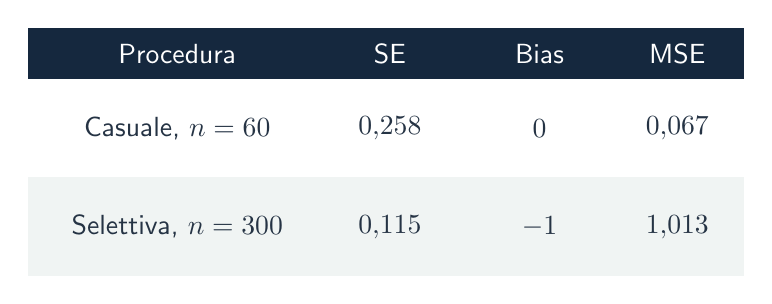
\begin{tikzpicture}[x=1cm,y=1cm]
\fill[Navy](.2,3.2) rectangle(9.3,3.85);
\foreach \x/\t in {2.1/Procedura,4.8/SE,6.7/Bias,8.45/MSE}
\node[pLabel,text=white] at(\x,3.52){\t};
\fill[white](.2,1.95) rectangle(9.3,3.2);
\fill[GeoTint](.2,.7) rectangle(9.3,1.95);
\node[pLabel] at(2.1,2.57){Casuale, $n=60$};
\node[pLabel] at(4.8,2.57){$0{,}258$};
\node[pLabel] at(6.7,2.57){$0$};
\node[pLabel] at(8.45,2.57){$0{,}067$};
\node[pLabel] at(2.1,1.32){Selettiva, $n=300$};
\node[pLabel] at(4.8,1.32){$0{,}115$};
\node[pLabel] at(6.7,1.32){$-1$};
\node[pLabel] at(8.45,1.32){$1{,}013$};
\end{tikzpicture}
\PSmall{Qui l'accuratezza riguarda lo scarto complessivo valutato dalla MSE. I valori provengono dalle distribuzioni teoriche delle due procedure.}

\end{minipage}% 
\end{lrbox}
\typeout{FULLBOX:020:L:\the\ht\PilotLeftBox:\the\dp\PilotLeftBox}
\begin{lrbox}{\PilotRightBox}%
\begin{minipage}[t]{7.55cm}\raggedright\color{Ink}\fontsize{11.3}{14.8}\selectfont

\PCode{R · confronto su SE e MSE}{020_confronto_procedure.R}
\PBody{La seconda procedura ha un SE minore e una MSE maggiore. La larghezza di un intervallo, da sola, lascia fuori il problema di selezione.}
\PInfo{Nella pratica il parametro è ignoto. Conoscere il disegno e documentare le esclusioni permette di discutere i limiti della stima.}

\end{minipage}% 
\end{lrbox}
\typeout{FULLBOX:020:R:\the\ht\PilotRightBox:\the\dp\PilotRightBox}
\begin{frame}[plain]\hypertarget{slide20}{}
\bookmark[level=1,page=20]{Precisione e accuratezza possono differire}
\begin{tikzpicture}[remember picture,overlay]
\PilotChrome{Precisione e accuratezza possono differire}{SELEZIONE E DISTORSIONE}{20}{La precisione descrive la dispersione delle stime. La MSE comprende anche la distorsione rispetto al parametro.}
\node[anchor=north west,inner sep=0] at ([xshift=0.96cm,yshift=-2.13cm]current page.north west) {\usebox{\PilotLeftBox}};
\node[anchor=north west,inner sep=0] at ([xshift=11.52cm,yshift=-2.13cm]current page.north west) {\usebox{\PilotRightBox}};

\end{tikzpicture}\end{frame}

% SLIDE 021 | I dati mancanti hanno una storia di raccolta
\begin{lrbox}{\PilotLeftBox}%
\begin{minipage}[t]{10.05cm}\raggedright\color{Ink}\fontsize{11.3}{14.8}\selectfont

\PLabel{Dal prelievo previsto al dato utilizzabile}
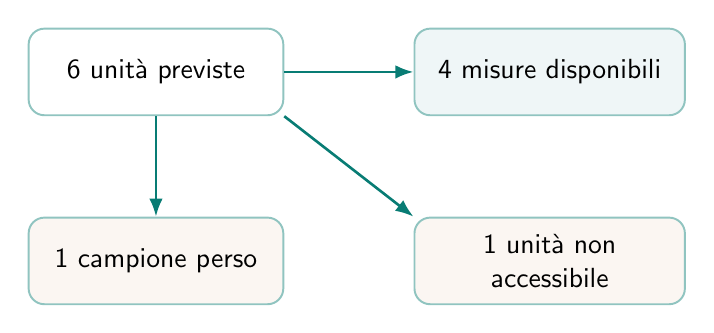
\begin{tikzpicture}[x=1cm,y=1cm]
\node[pFlow,text width=3cm] (p) at(2,3.3){6 unità previste};
\node[pFlow,text width=3.2cm,fill=GeoA!7] (o) at(7,3.3){4 misure disponibili};
\node[pFlow,text width=3cm,fill=GeoB!7] (l) at(2,.9){1 campione perso};
\node[pFlow,text width=3.2cm,fill=GeoB!7] (a) at(7,.9){1 unità non accessibile};
\draw[pEdge](p)--(o);\draw[pEdge](p)--(l);
\draw[pEdge](p.south east)--(a.north west);
\end{tikzpicture}
\PBody{Perdita accidentale e impossibilità di accesso possono avere conseguenze diverse. Registrare il motivo permette di discuterle.}

\end{minipage}% 
\end{lrbox}
\typeout{FULLBOX:021:L:\the\ht\PilotLeftBox:\the\dp\PilotLeftBox}
\begin{lrbox}{\PilotRightBox}%
\begin{minipage}[t]{7.55cm}\raggedright\color{Ink}\fontsize{11.3}{14.8}\selectfont

\PCode{R · conteggio degli esiti}{021_dati_mancanti.R}
\PSmall{\texttt{na.rm = TRUE} calcola la media delle misure disponibili. La rappresentatività delle unità restanti richiede un'analisi separata.}
\PInfo{Riportare unità previste, unità osservate e motivi delle esclusioni.}

\end{minipage}% 
\end{lrbox}
\typeout{FULLBOX:021:R:\the\ht\PilotRightBox:\the\dp\PilotRightBox}
\begin{frame}[plain]\hypertarget{slide21}{}
\bookmark[level=1,page=21]{I dati mancanti hanno una storia di raccolta}
\begin{tikzpicture}[remember picture,overlay]
\PilotChrome{I dati mancanti hanno una storia di raccolta}{SELEZIONE E DISTORSIONE}{21}{La gestione informatica dei valori mancanti va accompagnata dalla descrizione del processo che li ha prodotti.}
\node[anchor=north west,inner sep=0] at ([xshift=0.96cm,yshift=-2.13cm]current page.north west) {\usebox{\PilotLeftBox}};
\node[anchor=north west,inner sep=0] at ([xshift=11.52cm,yshift=-2.13cm]current page.north west) {\usebox{\PilotRightBox}};

\end{tikzpicture}\end{frame}

% SLIDE 022 | Il registro conserva il disegno del campione
\begin{lrbox}{\PilotLeftBox}%
\begin{minipage}[t]{10.05cm}\raggedright\color{Ink}\fontsize{11.3}{14.8}\selectfont

\PLabel{Informazioni da mantenere nella tabella}
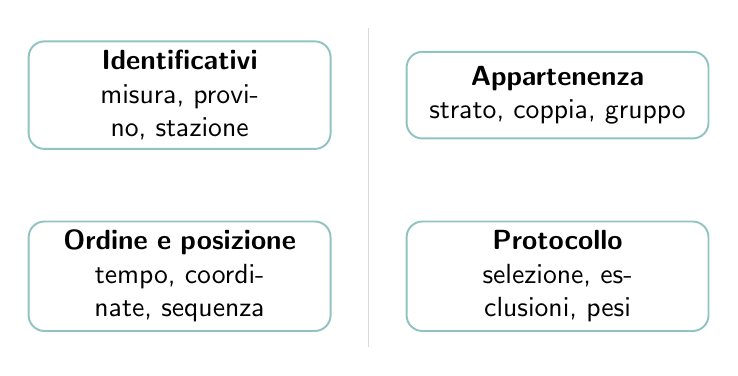
\begin{tikzpicture}[x=1cm,y=1cm]
\node[pFlow,text width=3.6cm] at(2.2,3.4){\textbf{Identificativi}\\misura, provino, stazione};
\node[pFlow,text width=3.6cm] at(7,3.4){\textbf{Appartenenza}\\strato, coppia, gruppo};
\node[pFlow,text width=3.6cm] at(2.2,1.1){\textbf{Ordine e posizione}\\tempo, coordinate, sequenza};
\node[pFlow,text width=3.6cm] at(7,1.1){\textbf{Protocollo}\\selezione, esclusioni, pesi};
\draw[Rule](4.6,.2)--(4.6,4.25);
\end{tikzpicture}
\PSmall{Il registro deve permettere di ricostruire le unità indipendenti e le relazioni fra osservazioni. I campi necessari dipendono dall'indagine.}

\end{minipage}% 
\end{lrbox}
\typeout{FULLBOX:022:L:\the\ht\PilotLeftBox:\the\dp\PilotLeftBox}
\begin{lrbox}{\PilotRightBox}%
\begin{minipage}[t]{7.55cm}\raggedright\color{Ink}\fontsize{11.3}{14.8}\selectfont

\PCode{R · identificativi e metadati}{022_registro.R}
\PBody{Tabelle con gli stessi numeri possono richiedere calcoli diversi se una contiene coppie e l'altra campioni indipendenti.}
\PInfo{Verificare duplicati, codici di stazione, ordine delle serie e corrispondenza fra coppie.}

\end{minipage}% 
\end{lrbox}
\typeout{FULLBOX:022:R:\the\ht\PilotRightBox:\the\dp\PilotRightBox}
\begin{frame}[plain]\hypertarget{slide22}{}
\bookmark[level=1,page=22]{Il registro conserva il disegno del campione}
\begin{tikzpicture}[remember picture,overlay]
\PilotChrome{Il registro conserva il disegno del campione}{SELEZIONE E DISTORSIONE}{22}{Perdere le informazioni sul disegno può impedire di calcolare correttamente l’incertezza anche quando i valori numerici sono integri.}
\node[anchor=north west,inner sep=0] at ([xshift=0.96cm,yshift=-2.13cm]current page.north west) {\usebox{\PilotLeftBox}};
\node[anchor=north west,inner sep=0] at ([xshift=11.52cm,yshift=-2.13cm]current page.north west) {\usebox{\PilotRightBox}};

\end{tikzpicture}\end{frame}

% SLIDE 023 | Laboratorio: precisione e selezione
\begin{lrbox}{\PilotLeftBox}%
\begin{minipage}[t]{10.05cm}\raggedright\color{Ink}\fontsize{11.3}{14.8}\selectfont

\PLab{https://marzione00.github.io/Lab_Geo/\#laboratorio/m05-selezione}{Esperimento · precisione e bias}
\[
\widehat\theta_{\mathrm C}\sim N\!\left(10,\frac4n\right),
\qquad
\widehat\theta_{\mathrm S}\sim N\!\left(10-b,\frac4n\right).
\]
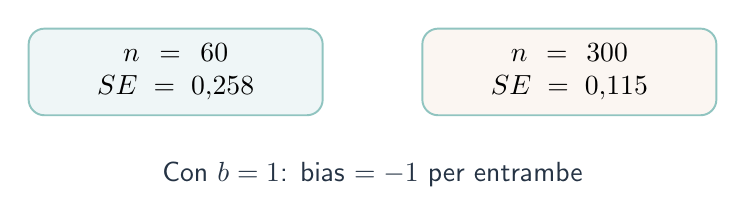
\begin{tikzpicture}[x=1cm,y=1cm]
\node[pFlow,text width=3.5cm,fill=GeoA!7] at(2.1,2.1){$n=60$\\$SE=0{,}258$};
\node[pFlow,text width=3.5cm,fill=GeoB!7] at(7.1,2.1){$n=300$\\$SE=0{,}115$};
\node[pLabel] at(4.6,.8){Con $b=1$: bias $=-1$ per entrambe};
\end{tikzpicture}
\PSmall{Il laboratorio genera direttamente $B$ stime normali per procedura. Rappresenta uno spostamento, senza simulare una selezione geografica.}

\end{minipage}% 
\end{lrbox}
\typeout{FULLBOX:023:L:\the\ht\PilotLeftBox:\the\dp\PilotLeftBox}
\begin{lrbox}{\PilotRightBox}%
\begin{minipage}[t]{7.55cm}\raggedright\color{Ink}\fontsize{11.3}{14.8}\selectfont

\PCode{R · confronto fra scenari}{023_lab_selezione.R}
\PBody{Annotare centro, dispersione e MSE. Ripetere con bias nullo e confrontare ciò che cambia.}
\PInfo{$n$ controlla la variabilità della stima. $B$ conta le stime simulate. Il parametro del sito \texttt{bias} è $b$: la distorsione effettiva vale $-b$.}

\end{minipage}% 
\end{lrbox}
\typeout{FULLBOX:023:R:\the\ht\PilotRightBox:\the\dp\PilotRightBox}
\begin{frame}[plain]\hypertarget{slide23}{}
\bookmark[level=1,page=23]{Laboratorio: precisione e selezione}
\begin{tikzpicture}[remember picture,overlay]
\PilotChrome{Laboratorio: precisione e selezione}{SELEZIONE E DISTORSIONE}{23}{Una simulazione si interpreta a partire dal meccanismo scritto nel codice e dal significato esatto dei parametri.}
\node[anchor=north west,inner sep=0] at ([xshift=0.96cm,yshift=-2.13cm]current page.north west) {\usebox{\PilotLeftBox}};
\node[anchor=north west,inner sep=0] at ([xshift=11.52cm,yshift=-2.13cm]current page.north west) {\usebox{\PilotRightBox}};

\end{tikzpicture}\end{frame}

% SLIDE 024 | n, G e B contano quantità diverse
\begin{lrbox}{\PilotLeftBox}%
\begin{minipage}[t]{10.05cm}\raggedright\color{Ink}\fontsize{11.3}{14.8}\selectfont

\PLabel{Le dimensioni del problema}
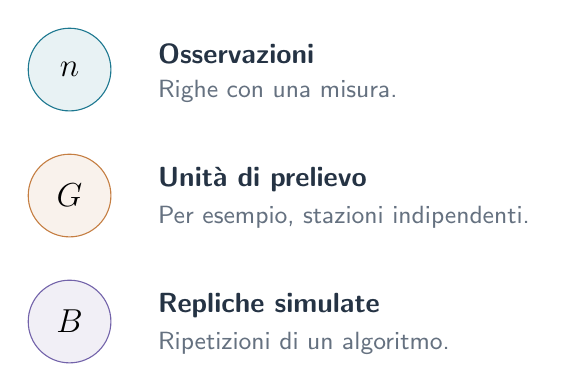
\begin{tikzpicture}[x=1cm,y=1cm]
\foreach \yy/\sim/\tit/\desc/\col in {
3.7/n/{Osservazioni}/{Righe con una misura.}/GeoA,
2.1/G/{Unità di prelievo}/{Per esempio, stazioni indipendenti.}/GeoB,
.5/B/{Repliche simulate}/{Ripetizioni di un algoritmo.}/GeoC}{
\node[circle,fill=\col!10,draw=\col,minimum size=1.05cm,font=\large] at(1,\yy){$\sim$};
\node[pLabel,anchor=west] at(2,\yy+.2){\textbf{\tit}};
\node[pNote,anchor=west] at(2,\yy-.28){\desc};
}
\end{tikzpicture}
\PSmall{Nel caso dei provini: 24 osservazioni in 6 stazioni. Il numero di ricampionamenti è una scelta del calcolo.}

\end{minipage}% 
\end{lrbox}
\typeout{FULLBOX:024:L:\the\ht\PilotLeftBox:\the\dp\PilotLeftBox}
\begin{lrbox}{\PilotRightBox}%
\begin{minipage}[t]{7.55cm}\raggedright\color{Ink}\fontsize{11.3}{14.8}\selectfont

\PCode{R · tre conteggi espliciti}{024_numerosita.R}
\PBody{Più $G$: nuove unità. Più $n$: anche misure nelle unità già note. Più $B$: repliche al computer.}
\PInfo{Per la stabilità numerica useremo anche $R=30$: ripetizioni complete del bootstrap sullo stesso campione.}

\end{minipage}% 
\end{lrbox}
\typeout{FULLBOX:024:R:\the\ht\PilotRightBox:\the\dp\PilotRightBox}
\begin{frame}[plain]\hypertarget{slide24}{}
\bookmark[level=1,page=24]{n, G e B contano quantità diverse}
\begin{tikzpicture}[remember picture,overlay]
\PilotChrome{n, G e B contano quantità diverse}{SELEZIONE E DISTORSIONE}{24}{Le repliche del computer stabilizzano il calcolo. La quantità di informazione dipende dai dati e dal disegno.}
\node[anchor=north west,inner sep=0] at ([xshift=0.96cm,yshift=-2.13cm]current page.north west) {\usebox{\PilotLeftBox}};
\node[anchor=north west,inner sep=0] at ([xshift=11.52cm,yshift=-2.13cm]current page.north west) {\usebox{\PilotRightBox}};

\end{tikzpicture}\end{frame}

% SLIDE 025 | Una distribuzione di stime richiede campioni ripetuti
\begin{lrbox}{\PilotLeftBox}%
\begin{minipage}[t]{10.05cm}\raggedright\color{Ink}\fontsize{11.3}{14.8}\selectfont

\PLabel{Dalle osservazioni alle statistiche}
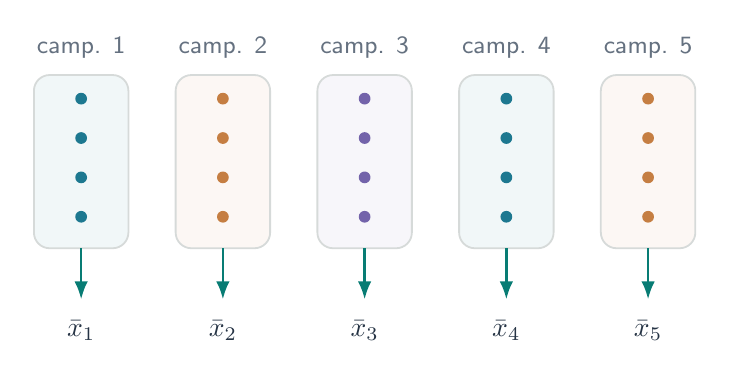
\begin{tikzpicture}[x=1cm,y=1cm]
\foreach \xx/\k/\col in {1.2/1/GeoA,3/2/GeoB,4.8/3/GeoC,6.6/4/GeoA,8.4/5/GeoB}{
\draw[pGroup,fill=\col!6](\xx-.6,1.4) rectangle(\xx+.6,3.6);
\node[pNote] at(\xx,3.95){camp. \k};
\foreach \yy in {1.8,2.3,2.8,3.3}\node[circle,fill=\col,inner sep=1.5pt] at(\xx,\yy){};
\draw[pEdge](\xx,1.4)--(\xx,.75);
\node[pLabel] at(\xx,.35){$\bar x_{\k}$};
}
\end{tikzpicture}
\PBody{Ogni colonna rappresenta un campione completo. Le cinque medie descrivono la variazione della stima fra queste ripetizioni.}

\end{minipage}% 
\end{lrbox}
\typeout{FULLBOX:025:L:\the\ht\PilotLeftBox:\the\dp\PilotLeftBox}
\begin{lrbox}{\PilotRightBox}%
\begin{minipage}[t]{7.55cm}\raggedright\color{Ink}\fontsize{11.3}{14.8}\selectfont

\PCode{R · una statistica per colonna}{025_ripetizioni.R}
\PSmall{\texttt{replicate()} ripete l'estrazione completa. \texttt{colMeans()} calcola la media di ogni campione. Riunire le 20 misure descriverebbe la distribuzione empirica dei dati individuali.}
\PInfo{Confronteremo la distribuzione dei dati individuali con quella della loro media.}

\end{minipage}% 
\end{lrbox}
\typeout{FULLBOX:025:R:\the\ht\PilotRightBox:\the\dp\PilotRightBox}
\begin{frame}[plain]\hypertarget{slide25}{}
\bookmark[level=1,page=25]{Una distribuzione di stime richiede campioni ripetuti}
\begin{tikzpicture}[remember picture,overlay]
\PilotChrome{Una distribuzione di stime richiede campioni ripetuti}{SELEZIONE E DISTORSIONE}{25}{La distribuzione campionaria riguarda una statistica calcolata su campioni ripetuti dello stesso disegno.}
\node[anchor=north west,inner sep=0] at ([xshift=0.96cm,yshift=-2.13cm]current page.north west) {\usebox{\PilotLeftBox}};
\node[anchor=north west,inner sep=0] at ([xshift=11.52cm,yshift=-2.13cm]current page.north west) {\usebox{\PilotRightBox}};

\end{tikzpicture}\end{frame}

% SLIDE 026 | Una media per ciascun campione
\begin{lrbox}{\PilotLeftBox}%
\begin{minipage}[t]{10.05cm}\raggedright\color{Ink}\fontsize{11.3}{14.8}\selectfont

\PLabel{La ripetizione riguarda l'intero campionamento}
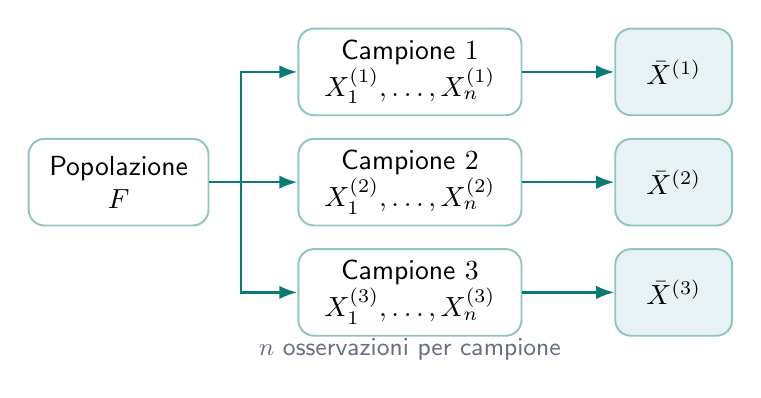
\begin{tikzpicture}[x=1cm,y=1cm]
\node[pFlow,text width=2.05cm] (p) at(1.3,2.0){Popolazione\\$F$};
\foreach \y/\lab in {3.4/1,2.0/2,.6/3}{
\node[pFlow,text width=2.6cm] (c\lab) at(5,\y){Campione $\lab$\\$X_1^{(\lab)},\ldots,X_n^{(\lab)}$};
\node[pFlow,text width=1.25cm,fill=GeoA!10] (m\lab) at(8.35,\y){$\bar X^{(\lab)}$};
\draw[pEdge](p.east)--++(.4,0)|-(c\lab.west);
\draw[pEdge](c\lab)--(m\lab);}
\node[pNote] at(5,-.13){$n$ osservazioni per campione};
\end{tikzpicture}
\PBody{La distribuzione campionaria descrive le medie ottenibili ripetendo lo stesso disegno, con popolazione e numerosità fissate.}

\end{minipage}% 
\end{lrbox}
\typeout{FULLBOX:026:L:\the\ht\PilotLeftBox:\the\dp\PilotLeftBox}
\begin{lrbox}{\PilotRightBox}%
\begin{minipage}[t]{7.55cm}\raggedright\color{Ink}\fontsize{11.3}{14.8}\selectfont

\PCode{R · quattro campioni esponenziali}{026_campioni.R}
\PBody{\texttt{replicate()} ripete un'espressione. \texttt{colMeans()} restituisce una media per colonna.}
\PInfo{Prima dell'osservazione, $\bar X$ è una variabile aleatoria. Dopo l'osservazione, $\bar x$ è il valore calcolato nel campione.}

\end{minipage}% 
\end{lrbox}
\typeout{FULLBOX:026:R:\the\ht\PilotRightBox:\the\dp\PilotRightBox}
\begin{frame}[plain]\hypertarget{slide26}{}
\bookmark[level=1,page=26]{Una media per ciascun campione}
\begin{tikzpicture}[remember picture,overlay]
\PilotChrome{Una media per ciascun campione}{DISTRIBUZIONI CAMPIONARIE}{26}{Ogni punto della distribuzione campionaria corrisponde a una statistica calcolata su un intero campione.}
\node[anchor=north west,inner sep=0] at ([xshift=0.96cm,yshift=-2.13cm]current page.north west) {\usebox{\PilotLeftBox}};
\node[anchor=north west,inner sep=0] at ([xshift=11.52cm,yshift=-2.13cm]current page.north west) {\usebox{\PilotRightBox}};

\end{tikzpicture}\end{frame}

% SLIDE 027 | Stessi momenti, forme diverse
\begin{lrbox}{\PilotLeftBox}%
\begin{minipage}[t]{10.05cm}\raggedright\color{Ink}\fontsize{11.3}{14.8}\selectfont

\PLabel{Le due popolazioni offerte nel laboratorio}
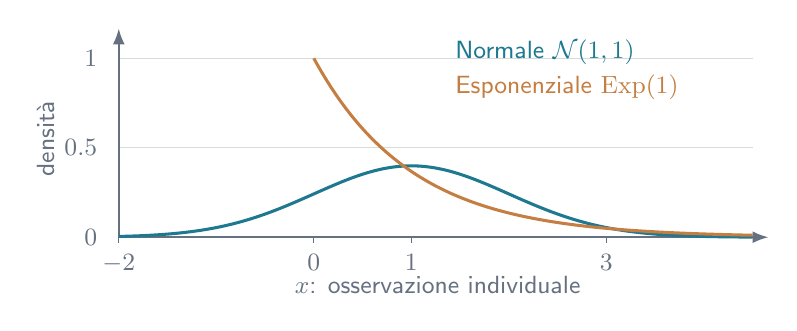
\begin{tikzpicture}[x=1cm,y=1cm]
\draw[Rule](.75,0.0000)--(8.8,0.0000);
\node[pNote,anchor=east] at(.60,0.0000){$ 0 $};
\draw[Rule](.75,1.1364)--(8.8,1.1364);
\node[pNote,anchor=east] at(.60,1.1364){$ 0.5 $};
\draw[Rule](.75,2.2727)--(8.8,2.2727);
\node[pNote,anchor=east] at(.60,2.2727){$ 1 $};
\draw[pAxis](.75,0)--(9,0);
\draw[pAxis](.75,0)--(.75,2.65);
\draw[Muted](0.7500,0)--(0.7500,-.07);
\node[pNote,below] at(0.7500,-.09){$ -2 $};
\draw[Muted](3.2269,0)--(3.2269,-.07);
\node[pNote,below] at(3.2269,-.09){$ 0 $};
\draw[Muted](4.4654,0)--(4.4654,-.07);
\node[pNote,below] at(4.4654,-.09){$ 1 $};
\draw[Muted](6.9423,0)--(6.9423,-.07);
\node[pNote,below] at(6.9423,-.09){$ 3 $};
\node[pNote] at(4.8,-.61){$x$: osservazione individuale};
\node[pNote,rotate=90] at(-.18,1.25){densità};
\draw[GeoA,line width=1.1pt,] plot coordinates{(0.75000,0.01007) (0.78096,0.01085) (0.81192,0.01169) (0.84288,0.01258) (0.87385,0.01353) (0.90481,0.01454) (0.93577,0.01562) (0.96673,0.01677) (0.99769,0.01799) (1.02865,0.01929) (1.05962,0.02067) (1.09058,0.02213) (1.12154,0.02368) (1.15250,0.02533) (1.18346,0.02707) (1.21442,0.02892) (1.24538,0.03087) (1.27635,0.03293) (1.30731,0.03511) (1.33827,0.03741) (1.36923,0.03984) (1.40019,0.04239) (1.43115,0.04508) (1.46212,0.04792) (1.49308,0.05090) (1.52404,0.05403) (1.55500,0.05731) (1.58596,0.06076) (1.61692,0.06438) (1.64788,0.06817) (1.67885,0.07214) (1.70981,0.07629) (1.74077,0.08062) (1.77173,0.08516) (1.80269,0.08989) (1.83365,0.09482) (1.86462,0.09996) (1.89558,0.10532) (1.92654,0.11089) (1.95750,0.11669) (1.98846,0.12271) (2.01942,0.12896) (2.05038,0.13544) (2.08135,0.14216) (2.11231,0.14913) (2.14327,0.15633) (2.17423,0.16378) (2.20519,0.17148) (2.23615,0.17943) (2.26712,0.18763) (2.29808,0.19608) (2.32904,0.20479) (2.36000,0.21375) (2.39096,0.22296) (2.42192,0.23242) (2.45288,0.24213) (2.48385,0.25209) (2.51481,0.26230) (2.54577,0.27275) (2.57673,0.28344) (2.60769,0.29436) (2.63865,0.30551) (2.66962,0.31689) (2.70058,0.32848) (2.73154,0.34029) (2.76250,0.35230) (2.79346,0.36451) (2.82442,0.37690) (2.85538,0.38947) (2.88635,0.40221) (2.91731,0.41511) (2.94827,0.42815) (2.97923,0.44133) (3.01019,0.45463) (3.04115,0.46804) (3.07212,0.48154) (3.10308,0.49512) (3.13404,0.50876) (3.16500,0.52246) (3.19596,0.53619) (3.22692,0.54993) (3.25788,0.56368) (3.28885,0.57741) (3.31981,0.59110) (3.35077,0.60474) (3.38173,0.61831) (3.41269,0.63178) (3.44365,0.64515) (3.47462,0.65839) (3.50558,0.67148) (3.53654,0.68440) (3.56750,0.69714) (3.59846,0.70967) (3.62942,0.72197) (3.66038,0.73403) (3.69135,0.74582) (3.72231,0.75733) (3.75327,0.76853) (3.78423,0.77942) (3.81519,0.78996) (3.84615,0.80015) (3.87712,0.80996) (3.90808,0.81938) (3.93904,0.82839) (3.97000,0.83698) (4.00096,0.84513) (4.03192,0.85282) (4.06288,0.86005) (4.09385,0.86679) (4.12481,0.87304) (4.15577,0.87879) (4.18673,0.88402) (4.21769,0.88873) (4.24865,0.89291) (4.27962,0.89654) (4.31058,0.89963) (4.34154,0.90216) (4.37250,0.90414) (4.40346,0.90555) (4.43442,0.90640) (4.46538,0.90669) (4.49635,0.90640) (4.52731,0.90555) (4.55827,0.90414) (4.58923,0.90216) (4.62019,0.89963) (4.65115,0.89654) (4.68212,0.89291) (4.71308,0.88873) (4.74404,0.88402) (4.77500,0.87879) (4.80596,0.87304) (4.83692,0.86679) (4.86788,0.86005) (4.89885,0.85282) (4.92981,0.84513) (4.96077,0.83698) (4.99173,0.82839) (5.02269,0.81938) (5.05365,0.80996) (5.08462,0.80015) (5.11558,0.78996) (5.14654,0.77942) (5.17750,0.76853) (5.20846,0.75733) (5.23942,0.74582) (5.27038,0.73403) (5.30135,0.72197) (5.33231,0.70967) (5.36327,0.69714) (5.39423,0.68440) (5.42519,0.67148) (5.45615,0.65839) (5.48712,0.64515) (5.51808,0.63178) (5.54904,0.61831) (5.58000,0.60474) (5.61096,0.59110) (5.64192,0.57741) (5.67288,0.56368) (5.70385,0.54993) (5.73481,0.53619) (5.76577,0.52246) (5.79673,0.50876) (5.82769,0.49512) (5.85865,0.48154) (5.88962,0.46804) (5.92058,0.45463) (5.95154,0.44133) (5.98250,0.42815) (6.01346,0.41511) (6.04442,0.40221) (6.07538,0.38947) (6.10635,0.37690) (6.13731,0.36451) (6.16827,0.35230) (6.19923,0.34029) (6.23019,0.32848) (6.26115,0.31689) (6.29212,0.30551) (6.32308,0.29436) (6.35404,0.28344) (6.38500,0.27275) (6.41596,0.26230) (6.44692,0.25209) (6.47788,0.24213) (6.50885,0.23242) (6.53981,0.22296) (6.57077,0.21375) (6.60173,0.20479) (6.63269,0.19608) (6.66365,0.18763) (6.69462,0.17943) (6.72558,0.17148) (6.75654,0.16378) (6.78750,0.15633) (6.81846,0.14913) (6.84942,0.14216) (6.88038,0.13544) (6.91135,0.12896) (6.94231,0.12271) (6.97327,0.11669) (7.00423,0.11089) (7.03519,0.10532) (7.06615,0.09996) (7.09712,0.09482) (7.12808,0.08989) (7.15904,0.08516) (7.19000,0.08062) (7.22096,0.07629) (7.25192,0.07214) (7.28288,0.06817) (7.31385,0.06438) (7.34481,0.06076) (7.37577,0.05731) (7.40673,0.05403) (7.43769,0.05090) (7.46865,0.04792) (7.49962,0.04508) (7.53058,0.04239) (7.56154,0.03984) (7.59250,0.03741) (7.62346,0.03511) (7.65442,0.03293) (7.68538,0.03087) (7.71635,0.02892) (7.74731,0.02707) (7.77827,0.02533) (7.80923,0.02368) (7.84019,0.02213) (7.87115,0.02067) (7.90212,0.01929) (7.93308,0.01799) (7.96404,0.01677) (7.99500,0.01562) (8.02596,0.01454) (8.05692,0.01353) (8.08788,0.01258) (8.11885,0.01169) (8.14981,0.01085) (8.18077,0.01007) (8.21173,0.00934) (8.24269,0.00866) (8.27365,0.00802) (8.30462,0.00742) (8.33558,0.00687) (8.36654,0.00635) (8.39750,0.00587) (8.42846,0.00542) (8.45942,0.00500) (8.49038,0.00461) (8.52135,0.00425) (8.55231,0.00391) (8.58327,0.00360) (8.61423,0.00332) (8.64519,0.00305) (8.67615,0.00280) (8.70712,0.00257) (8.73808,0.00236) (8.76904,0.00216) (8.80000,0.00198)};
\draw[GeoB,line width=1.1pt,] plot coordinates{(3.22692,2.27273) (3.25788,2.21661) (3.28885,2.16189) (3.31981,2.10851) (3.35077,2.05645) (3.38173,2.00567) (3.41269,1.95615) (3.44365,1.90786) (3.47462,1.86075) (3.50558,1.81481) (3.53654,1.77000) (3.56750,1.72630) (3.59846,1.68368) (3.62942,1.64211) (3.66038,1.60156) (3.69135,1.56202) (3.72231,1.52345) (3.75327,1.48584) (3.78423,1.44915) (3.81519,1.41338) (3.84615,1.37848) (3.87712,1.34444) (3.90808,1.31125) (3.93904,1.27887) (3.97000,1.24730) (4.00096,1.21650) (4.03192,1.18647) (4.06288,1.15717) (4.09385,1.12860) (4.12481,1.10074) (4.15577,1.07356) (4.18673,1.04705) (4.21769,1.02120) (4.24865,0.99599) (4.27962,0.97140) (4.31058,0.94741) (4.34154,0.92402) (4.37250,0.90121) (4.40346,0.87896) (4.43442,0.85726) (4.46538,0.83609) (4.49635,0.81545) (4.52731,0.79531) (4.55827,0.77568) (4.58923,0.75653) (4.62019,0.73785) (4.65115,0.71963) (4.68212,0.70186) (4.71308,0.68453) (4.74404,0.66763) (4.77500,0.65115) (4.80596,0.63507) (4.83692,0.61939) (4.86788,0.60410) (4.89885,0.58918) (4.92981,0.57464) (4.96077,0.56045) (4.99173,0.54661) (5.02269,0.53311) (5.05365,0.51995) (5.08462,0.50711) (5.11558,0.49459) (5.14654,0.48238) (5.17750,0.47047) (5.20846,0.45886) (5.23942,0.44753) (5.27038,0.43648) (5.30135,0.42570) (5.33231,0.41519) (5.36327,0.40494) (5.39423,0.39494) (5.42519,0.38519) (5.45615,0.37568) (5.48712,0.36640) (5.51808,0.35736) (5.54904,0.34853) (5.58000,0.33993) (5.61096,0.33154) (5.64192,0.32335) (5.67288,0.31537) (5.70385,0.30758) (5.73481,0.29999) (5.76577,0.29258) (5.79673,0.28536) (5.82769,0.27831) (5.85865,0.27144) (5.88962,0.26474) (5.92058,0.25820) (5.95154,0.25183) (5.98250,0.24561) (6.01346,0.23954) (6.04442,0.23363) (6.07538,0.22786) (6.10635,0.22224) (6.13731,0.21675) (6.16827,0.21140) (6.19923,0.20618) (6.23019,0.20109) (6.26115,0.19612) (6.29212,0.19128) (6.32308,0.18656) (6.35404,0.18195) (6.38500,0.17746) (6.41596,0.17308) (6.44692,0.16880) (6.47788,0.16464) (6.50885,0.16057) (6.53981,0.15661) (6.57077,0.15274) (6.60173,0.14897) (6.63269,0.14529) (6.66365,0.14170) (6.69462,0.13820) (6.72558,0.13479) (6.75654,0.13146) (6.78750,0.12822) (6.81846,0.12505) (6.84942,0.12197) (6.88038,0.11895) (6.91135,0.11602) (6.94231,0.11315) (6.97327,0.11036) (7.00423,0.10763) (7.03519,0.10498) (7.06615,0.10238) (7.09712,0.09986) (7.12808,0.09739) (7.15904,0.09499) (7.19000,0.09264) (7.22096,0.09035) (7.25192,0.08812) (7.28288,0.08595) (7.31385,0.08383) (7.34481,0.08176) (7.37577,0.07974) (7.40673,0.07777) (7.43769,0.07585) (7.46865,0.07398) (7.49962,0.07215) (7.53058,0.07037) (7.56154,0.06863) (7.59250,0.06694) (7.62346,0.06528) (7.65442,0.06367) (7.68538,0.06210) (7.71635,0.06057) (7.74731,0.05907) (7.77827,0.05761) (7.80923,0.05619) (7.84019,0.05480) (7.87115,0.05345) (7.90212,0.05213) (7.93308,0.05084) (7.96404,0.04959) (7.99500,0.04836) (8.02596,0.04717) (8.05692,0.04600) (8.08788,0.04487) (8.11885,0.04376) (8.14981,0.04268) (8.18077,0.04163) (8.21173,0.04060) (8.24269,0.03960) (8.27365,0.03862) (8.30462,0.03767) (8.33558,0.03674) (8.36654,0.03583) (8.39750,0.03494) (8.42846,0.03408) (8.45942,0.03324) (8.49038,0.03242) (8.52135,0.03162) (8.55231,0.03084) (8.58327,0.03008) (8.61423,0.02933) (8.64519,0.02861) (8.67615,0.02790) (8.70712,0.02721) (8.73808,0.02654) (8.76904,0.02589) (8.80000,0.02525)};
\node[pNote,text=GeoA,anchor=west] at(4.9,2.35){Normale $\mathcal N(1,1)$};
\node[pNote,text=GeoB,anchor=west] at(4.9,1.91){Esponenziale $\mathrm{Exp}(1)$};
\end{tikzpicture}
\[
\mathbb E(X)=1,\qquad \operatorname{Var}(X)=1.
\]
\PSmall{La normale ammette anche valori negativi. Qui confrontiamo modelli matematici adimensionali, senza attribuire loro una grandezza fisica positiva.}

\end{minipage}% 
\end{lrbox}
\typeout{FULLBOX:027:L:\the\ht\PilotLeftBox:\the\dp\PilotLeftBox}
\begin{lrbox}{\PilotRightBox}%
\begin{minipage}[t]{7.55cm}\raggedright\color{Ink}\fontsize{11.3}{14.8}\selectfont

\PCode{R · due generatori}{027_popolazioni.R}
\PBody{I valori osservati di media e varianza oscillano. I parametri delle due popolazioni restano uguali a uno.}
\PInfo{La forma della distribuzione dei dati può influire sulla distribuzione della media quando il campione è piccolo.}

\end{minipage}% 
\end{lrbox}
\typeout{FULLBOX:027:R:\the\ht\PilotRightBox:\the\dp\PilotRightBox}
\begin{frame}[plain]\hypertarget{slide27}{}
\bookmark[level=1,page=27]{Stessi momenti, forme diverse}
\begin{tikzpicture}[remember picture,overlay]
\PilotChrome{Stessi momenti, forme diverse}{DISTRIBUZIONI CAMPIONARIE}{27}{La media e la varianza della popolazione non ne determinano da sole la forma.}
\node[anchor=north west,inner sep=0] at ([xshift=0.96cm,yshift=-2.13cm]current page.north west) {\usebox{\PilotLeftBox}};
\node[anchor=north west,inner sep=0] at ([xshift=11.52cm,yshift=-2.13cm]current page.north west) {\usebox{\PilotRightBox}};

\end{tikzpicture}\end{frame}

% SLIDE 028 | Il valore atteso della media
\begin{lrbox}{\PilotLeftBox}%
\begin{minipage}[t]{10.05cm}\raggedright\color{Ink}\fontsize{11.3}{14.8}\selectfont

\PLabel{La linearità dell'aspettazione}
\[
\begin{aligned}
\mathbb E(\bar X)
&=\mathbb E\!\left(\frac1n\sum_{i=1}^n X_i\right)\\
&=\frac1n\sum_{i=1}^n\mathbb E(X_i)
=\frac{n\mu}{n}=\mu.
\end{aligned}
\]
\begin{tikzpicture}[x=1cm,y=1cm]
\node[pFlow,text width=3.2cm] (a) at(1.9,1){Ogni osservazione\\ha media $\mu$};
\node[pFlow,text width=3.6cm,fill=GeoA!10] (b) at(7.1,1){Anche $\bar X$\\ha media $\mu$};
\draw[pEdge](a)--node[pNote,above]{media}(b);
\end{tikzpicture}
\PSmall{Sono sufficienti valori attesi finiti e uguali. Questa derivazione non usa l'indipendenza.}

\end{minipage}% 
\end{lrbox}
\typeout{FULLBOX:028:L:\the\ht\PilotLeftBox:\the\dp\PilotLeftBox}
\begin{lrbox}{\PilotRightBox}%
\begin{minipage}[t]{7.55cm}\raggedright\color{Ink}\fontsize{11.3}{14.8}\selectfont

\PCode{R · medie attese dei contributi}{028_valore_atteso.R}
\PBody{Con medie differenti $\mu_i$, il risultato diventa $\mathbb E(\bar X)=n^{-1}\sum_i\mu_i$.}
\PInfo{La non distorsione riguarda il valore atteso dello stimatore. Una singola media campionaria può trovarsi sopra o sotto il parametro.}

\end{minipage}% 
\end{lrbox}
\typeout{FULLBOX:028:R:\the\ht\PilotRightBox:\the\dp\PilotRightBox}
\begin{frame}[plain]\hypertarget{slide28}{}
\bookmark[level=1,page=28]{Il valore atteso della media}
\begin{tikzpicture}[remember picture,overlay]
\PilotChrome{Il valore atteso della media}{DISTRIBUZIONI CAMPIONARIE}{28}{La media è non distorta per una media comune finita, anche quando le osservazioni sono dipendenti.}
\node[anchor=north west,inner sep=0] at ([xshift=0.96cm,yshift=-2.13cm]current page.north west) {\usebox{\PilotLeftBox}};
\node[anchor=north west,inner sep=0] at ([xshift=11.52cm,yshift=-2.13cm]current page.north west) {\usebox{\PilotRightBox}};

\end{tikzpicture}\end{frame}

% SLIDE 029 | Da dati normali a medie normali
\begin{lrbox}{\PilotLeftBox}%
\begin{minipage}[t]{10.05cm}\raggedright\color{Ink}\fontsize{11.3}{14.8}\selectfont

\PLabel{Un risultato esatto sotto indipendenza}
\begin{tikzpicture}[x=1cm,y=1cm]
\draw[Rule](.75,0.0000)--(8.8,0.0000);
\node[pNote,anchor=east] at(.60,0.0000){$ 0 $};
\draw[Rule](.75,0.7353)--(8.8,0.7353);
\node[pNote,anchor=east] at(.60,0.7353){$ 1 $};
\draw[Rule](.75,1.4706)--(8.8,1.4706);
\node[pNote,anchor=east] at(.60,1.4706){$ 2 $};
\draw[Rule](.75,2.2059)--(8.8,2.2059);
\node[pNote,anchor=east] at(.60,2.2059){$ 3 $};
\draw[pAxis](.75,0)--(9,0);
\draw[pAxis](.75,0)--(.75,2.65);
\draw[Muted](1.4208,0)--(1.4208,-.07);
\node[pNote,below] at(1.4208,-.09){$ 0 $};
\draw[Muted](3.0979,0)--(3.0979,-.07);
\node[pNote,below] at(3.0979,-.09){$ 0.5 $};
\draw[Muted](4.7750,0)--(4.7750,-.07);
\node[pNote,below] at(4.7750,-.09){$ 1 $};
\draw[Muted](6.4521,0)--(6.4521,-.07);
\node[pNote,below] at(6.4521,-.09){$ 1.5 $};
\draw[Muted](8.1292,0)--(8.1292,-.07);
\node[pNote,below] at(8.1292,-.09){$ 2 $};
\node[pNote] at(4.8,-.61){$\bar x$: media di un campione};
\node[pNote,rotate=90] at(-.18,1.25){densità};
\draw[GeoB,line width=1.1pt,] plot coordinates{(0.75000,0.00018) (0.78354,0.00021) (0.81708,0.00024) (0.85062,0.00028) (0.88417,0.00032) (0.91771,0.00036) (0.95125,0.00042) (0.98479,0.00048) (1.01833,0.00055) (1.05187,0.00063) (1.08542,0.00071) (1.11896,0.00081) (1.15250,0.00093) (1.18604,0.00106) (1.21958,0.00120) (1.25312,0.00136) (1.28667,0.00154) (1.32021,0.00175) (1.35375,0.00198) (1.38729,0.00223) (1.42083,0.00252) (1.45437,0.00284) (1.48792,0.00319) (1.52146,0.00359) (1.55500,0.00403) (1.58854,0.00452) (1.62208,0.00506) (1.65562,0.00567) (1.68917,0.00633) (1.72271,0.00707) (1.75625,0.00788) (1.78979,0.00877) (1.82333,0.00975) (1.85688,0.01083) (1.89042,0.01202) (1.92396,0.01331) (1.95750,0.01473) (1.99104,0.01629) (2.02458,0.01798) (2.05812,0.01983) (2.09167,0.02184) (2.12521,0.02403) (2.15875,0.02640) (2.19229,0.02897) (2.22583,0.03176) (2.25937,0.03477) (2.29292,0.03802) (2.32646,0.04153) (2.36000,0.04530) (2.39354,0.04936) (2.42708,0.05372) (2.46062,0.05839) (2.49417,0.06340) (2.52771,0.06874) (2.56125,0.07445) (2.59479,0.08054) (2.62833,0.08702) (2.66187,0.09391) (2.69542,0.10123) (2.72896,0.10898) (2.76250,0.11719) (2.79604,0.12586) (2.82958,0.13501) (2.86312,0.14466) (2.89667,0.15481) (2.93021,0.16547) (2.96375,0.17665) (2.99729,0.18837) (3.03083,0.20061) (3.06437,0.21340) (3.09792,0.22674) (3.13146,0.24061) (3.16500,0.25503) (3.19854,0.26999) (3.23208,0.28548) (3.26562,0.30150) (3.29917,0.31804) (3.33271,0.33509) (3.36625,0.35262) (3.39979,0.37062) (3.43333,0.38908) (3.46687,0.40797) (3.50042,0.42726) (3.53396,0.44692) (3.56750,0.46693) (3.60104,0.48725) (3.63458,0.50785) (3.66812,0.52868) (3.70167,0.54971) (3.73521,0.57088) (3.76875,0.59217) (3.80229,0.61350) (3.83583,0.63485) (3.86937,0.65615) (3.90292,0.67735) (3.93646,0.69840) (3.97000,0.71923) (4.00354,0.73980) (4.03708,0.76005) (4.07062,0.77992) (4.10417,0.79934) (4.13771,0.81826) (4.17125,0.83663) (4.20479,0.85439) (4.23833,0.87147) (4.27187,0.88783) (4.30542,0.90342) (4.33896,0.91817) (4.37250,0.93205) (4.40604,0.94500) (4.43958,0.95698) (4.47312,0.96795) (4.50667,0.97788) (4.54021,0.98672) (4.57375,0.99445) (4.60729,1.00103) (4.64083,1.00645) (4.67437,1.01069) (4.70792,1.01372) (4.74146,1.01555) (4.77500,1.01616) (4.80854,1.01555) (4.84208,1.01372) (4.87562,1.01069) (4.90917,1.00645) (4.94271,1.00103) (4.97625,0.99445) (5.00979,0.98672) (5.04333,0.97788) (5.07687,0.96795) (5.11042,0.95698) (5.14396,0.94500) (5.17750,0.93205) (5.21104,0.91817) (5.24458,0.90342) (5.27813,0.88783) (5.31167,0.87147) (5.34521,0.85439) (5.37875,0.83663) (5.41229,0.81826) (5.44583,0.79934) (5.47937,0.77992) (5.51292,0.76005) (5.54646,0.73980) (5.58000,0.71923) (5.61354,0.69840) (5.64708,0.67735) (5.68063,0.65615) (5.71417,0.63485) (5.74771,0.61350) (5.78125,0.59217) (5.81479,0.57088) (5.84833,0.54971) (5.88187,0.52868) (5.91542,0.50785) (5.94896,0.48725) (5.98250,0.46693) (6.01604,0.44692) (6.04958,0.42726) (6.08312,0.40797) (6.11667,0.38908) (6.15021,0.37062) (6.18375,0.35262) (6.21729,0.33509) (6.25083,0.31804) (6.28437,0.30150) (6.31792,0.28548) (6.35146,0.26999) (6.38500,0.25503) (6.41854,0.24061) (6.45208,0.22674) (6.48562,0.21340) (6.51917,0.20061) (6.55271,0.18837) (6.58625,0.17665) (6.61979,0.16547) (6.65333,0.15481) (6.68687,0.14466) (6.72042,0.13501) (6.75396,0.12586) (6.78750,0.11719) (6.82104,0.10898) (6.85458,0.10123) (6.88812,0.09391) (6.92167,0.08702) (6.95521,0.08054) (6.98875,0.07445) (7.02229,0.06874) (7.05583,0.06340) (7.08937,0.05839) (7.12292,0.05372) (7.15646,0.04936) (7.19000,0.04530) (7.22354,0.04153) (7.25708,0.03802) (7.29062,0.03477) (7.32417,0.03176) (7.35771,0.02897) (7.39125,0.02640) (7.42479,0.02403) (7.45833,0.02184) (7.49187,0.01983) (7.52542,0.01798) (7.55896,0.01629) (7.59250,0.01473) (7.62604,0.01331) (7.65958,0.01202) (7.69312,0.01083) (7.72667,0.00975) (7.76021,0.00877) (7.79375,0.00788) (7.82729,0.00707) (7.86083,0.00633) (7.89437,0.00567) (7.92792,0.00506) (7.96146,0.00452) (7.99500,0.00403) (8.02854,0.00359) (8.06208,0.00319) (8.09562,0.00284) (8.12917,0.00252) (8.16271,0.00223) (8.19625,0.00198) (8.22979,0.00175) (8.26333,0.00154) (8.29688,0.00136) (8.33042,0.00120) (8.36396,0.00106) (8.39750,0.00093) (8.43104,0.00081) (8.46458,0.00071) (8.49812,0.00063) (8.53167,0.00055) (8.56521,0.00048) (8.59875,0.00042) (8.63229,0.00036) (8.66583,0.00032) (8.69937,0.00028) (8.73292,0.00024) (8.76646,0.00021) (8.80000,0.00018)};
\draw[GeoA,line width=1.1pt,] plot coordinates{(0.75000,0.00000) (0.78354,0.00000) (0.81708,0.00000) (0.85062,0.00000) (0.88417,0.00000) (0.91771,0.00000) (0.95125,0.00000) (0.98479,0.00000) (1.01833,0.00000) (1.05187,0.00000) (1.08542,0.00000) (1.11896,0.00000) (1.15250,0.00000) (1.18604,0.00000) (1.21958,0.00000) (1.25312,0.00000) (1.28667,0.00000) (1.32021,0.00000) (1.35375,0.00000) (1.38729,0.00000) (1.42083,0.00000) (1.45437,0.00000) (1.48792,0.00000) (1.52146,0.00000) (1.55500,0.00000) (1.58854,0.00000) (1.62208,0.00000) (1.65562,0.00000) (1.68917,0.00000) (1.72271,0.00000) (1.75625,0.00000) (1.78979,0.00000) (1.82333,0.00000) (1.85688,0.00000) (1.89042,0.00000) (1.92396,0.00000) (1.95750,0.00000) (1.99104,0.00000) (2.02458,0.00000) (2.05812,0.00000) (2.09167,0.00000) (2.12521,0.00000) (2.15875,0.00000) (2.19229,0.00000) (2.22583,0.00000) (2.25937,0.00000) (2.29292,0.00000) (2.32646,0.00000) (2.36000,0.00000) (2.39354,0.00000) (2.42708,0.00000) (2.46062,0.00000) (2.49417,0.00000) (2.52771,0.00000) (2.56125,0.00000) (2.59479,0.00001) (2.62833,0.00001) (2.66187,0.00002) (2.69542,0.00002) (2.72896,0.00003) (2.76250,0.00005) (2.79604,0.00007) (2.82958,0.00009) (2.86312,0.00013) (2.89667,0.00019) (2.93021,0.00026) (2.96375,0.00036) (2.99729,0.00050) (3.03083,0.00068) (3.06437,0.00093) (3.09792,0.00126) (3.13146,0.00169) (3.16500,0.00226) (3.19854,0.00301) (3.23208,0.00398) (3.26562,0.00523) (3.29917,0.00682) (3.33271,0.00886) (3.36625,0.01143) (3.39979,0.01467) (3.43333,0.01870) (3.46687,0.02370) (3.50042,0.02986) (3.53396,0.03739) (3.56750,0.04655) (3.60104,0.05760) (3.63458,0.07085) (3.66812,0.08662) (3.70167,0.10527) (3.73521,0.12717) (3.76875,0.15270) (3.80229,0.18227) (3.83583,0.21626) (3.86937,0.25506) (3.90292,0.29902) (3.93646,0.34845) (3.97000,0.40363) (4.00354,0.46475) (4.03708,0.53193) (4.07062,0.60517) (4.10417,0.68437) (4.13771,0.76932) (4.17125,0.85963) (4.20479,0.95480) (4.23833,1.05417) (4.27187,1.15691) (4.30542,1.26206) (4.33896,1.36855) (4.37250,1.47513) (4.40604,1.58051) (4.43958,1.68329) (4.47312,1.78202) (4.50667,1.87526) (4.54021,1.96158) (4.57375,2.03959) (4.60729,2.10802) (4.64083,2.16571) (4.67437,2.21167) (4.70792,2.24510) (4.74146,2.26539) (4.77500,2.27220) (4.80854,2.26539) (4.84208,2.24510) (4.87562,2.21167) (4.90917,2.16571) (4.94271,2.10802) (4.97625,2.03959) (5.00979,1.96158) (5.04333,1.87526) (5.07687,1.78202) (5.11042,1.68329) (5.14396,1.58051) (5.17750,1.47513) (5.21104,1.36855) (5.24458,1.26206) (5.27813,1.15691) (5.31167,1.05417) (5.34521,0.95480) (5.37875,0.85963) (5.41229,0.76932) (5.44583,0.68437) (5.47937,0.60517) (5.51292,0.53193) (5.54646,0.46475) (5.58000,0.40363) (5.61354,0.34845) (5.64708,0.29902) (5.68063,0.25506) (5.71417,0.21626) (5.74771,0.18227) (5.78125,0.15270) (5.81479,0.12717) (5.84833,0.10527) (5.88187,0.08662) (5.91542,0.07085) (5.94896,0.05760) (5.98250,0.04655) (6.01604,0.03739) (6.04958,0.02986) (6.08312,0.02370) (6.11667,0.01870) (6.15021,0.01467) (6.18375,0.01143) (6.21729,0.00886) (6.25083,0.00682) (6.28437,0.00523) (6.31792,0.00398) (6.35146,0.00301) (6.38500,0.00226) (6.41854,0.00169) (6.45208,0.00126) (6.48562,0.00093) (6.51917,0.00068) (6.55271,0.00050) (6.58625,0.00036) (6.61979,0.00026) (6.65333,0.00019) (6.68687,0.00013) (6.72042,0.00009) (6.75396,0.00007) (6.78750,0.00005) (6.82104,0.00003) (6.85458,0.00002) (6.88812,0.00002) (6.92167,0.00001) (6.95521,0.00001) (6.98875,0.00000) (7.02229,0.00000) (7.05583,0.00000) (7.08937,0.00000) (7.12292,0.00000) (7.15646,0.00000) (7.19000,0.00000) (7.22354,0.00000) (7.25708,0.00000) (7.29062,0.00000) (7.32417,0.00000) (7.35771,0.00000) (7.39125,0.00000) (7.42479,0.00000) (7.45833,0.00000) (7.49187,0.00000) (7.52542,0.00000) (7.55896,0.00000) (7.59250,0.00000) (7.62604,0.00000) (7.65958,0.00000) (7.69312,0.00000) (7.72667,0.00000) (7.76021,0.00000) (7.79375,0.00000) (7.82729,0.00000) (7.86083,0.00000) (7.89437,0.00000) (7.92792,0.00000) (7.96146,0.00000) (7.99500,0.00000) (8.02854,0.00000) (8.06208,0.00000) (8.09562,0.00000) (8.12917,0.00000) (8.16271,0.00000) (8.19625,0.00000) (8.22979,0.00000) (8.26333,0.00000) (8.29688,0.00000) (8.33042,0.00000) (8.36396,0.00000) (8.39750,0.00000) (8.43104,0.00000) (8.46458,0.00000) (8.49812,0.00000) (8.53167,0.00000) (8.56521,0.00000) (8.59875,0.00000) (8.63229,0.00000) (8.66583,0.00000) (8.69937,0.00000) (8.73292,0.00000) (8.76646,0.00000) (8.80000,0.00000)};
\node[pNote,text=GeoB] at(7.5,2.25){$n=12$};
\node[pNote,text=GeoA] at(7.5,1.82){$n=60$};
\end{tikzpicture}
\[
X_i\overset{\mathrm{iid}}\sim\mathcal N(\mu,\sigma^2)
\quad\Longrightarrow\quad
\bar X\sim\mathcal N\!\left(\mu,\frac{\sigma^2}{n}\right).
\]
\PSmall{Nel grafico $\mu=\sigma=1$. La media mantiene il centro e ha dispersione minore.}

\end{minipage}% 
\end{lrbox}
\typeout{FULLBOX:029:L:\the\ht\PilotLeftBox:\the\dp\PilotLeftBox}
\begin{lrbox}{\PilotRightBox}%
\begin{minipage}[t]{7.55cm}\raggedright\color{Ink}\fontsize{11.3}{14.8}\selectfont

\PCode{R · probabilità per una media}{029_media_normale.R}
\PBody{\texttt{pnorm()} richiede la deviazione standard. Per $\bar X$ usiamo $1/\sqrt n$, con $\sigma=1$.}
\PInfo{Il risultato vale per ogni $n$ nel modello normale indipendente. Non richiede un'approssimazione asintotica.}

\end{minipage}% 
\end{lrbox}
\typeout{FULLBOX:029:R:\the\ht\PilotRightBox:\the\dp\PilotRightBox}
\begin{frame}[plain]\hypertarget{slide29}{}
\bookmark[level=1,page=29]{Da dati normali a medie normali}
\begin{tikzpicture}[remember picture,overlay]
\PilotChrome{Da dati normali a medie normali}{DISTRIBUZIONI CAMPIONARIE}{29}{La normale della media ha varianza σ²/n quando i dati sono normali e indipendenti.}
\node[anchor=north west,inner sep=0] at ([xshift=0.96cm,yshift=-2.13cm]current page.north west) {\usebox{\PilotLeftBox}};
\node[anchor=north west,inner sep=0] at ([xshift=11.52cm,yshift=-2.13cm]current page.north west) {\usebox{\PilotRightBox}};

\end{tikzpicture}\end{frame}

% SLIDE 030 | Le medie di dati asimmetrici
\begin{lrbox}{\PilotLeftBox}%
\begin{minipage}[t]{10.05cm}\raggedright\color{Ink}\fontsize{11.3}{14.8}\selectfont

\PLabel{Esponenziale di media e varianza unitarie}
\begin{tikzpicture}[x=1cm,y=1cm]
\draw[Rule](.75,0.0000)--(8.8,0.0000);
\node[pNote,anchor=east] at(.60,0.0000){$ 0 $};
\draw[Rule](.75,0.7353)--(8.8,0.7353);
\node[pNote,anchor=east] at(.60,0.7353){$ 1 $};
\draw[Rule](.75,1.4706)--(8.8,1.4706);
\node[pNote,anchor=east] at(.60,1.4706){$ 2 $};
\draw[Rule](.75,2.2059)--(8.8,2.2059);
\node[pNote,anchor=east] at(.60,2.2059){$ 3 $};
\draw[pAxis](.75,0)--(9,0);
\draw[pAxis](.75,0)--(.75,2.65);
\draw[Muted](0.7500,0)--(0.7500,-.07);
\node[pNote,below] at(0.7500,-.09){$ 0 $};
\draw[Muted](2.5000,0)--(2.5000,-.07);
\node[pNote,below] at(2.5000,-.09){$ 0.5 $};
\draw[Muted](4.2500,0)--(4.2500,-.07);
\node[pNote,below] at(4.2500,-.09){$ 1 $};
\draw[Muted](6.0000,0)--(6.0000,-.07);
\node[pNote,below] at(6.0000,-.09){$ 1.5 $};
\draw[Muted](7.7500,0)--(7.7500,-.07);
\node[pNote,below] at(7.7500,-.09){$ 2 $};
\node[pNote] at(4.8,-.61){$\bar x$: media di un campione};
\node[pNote,rotate=90] at(-.18,1.25){densità};
\draw[GeoB,line width=1.1pt,] plot coordinates{(0.75000,0.00000) (0.78500,0.00000) (0.82000,0.00000) (0.85500,0.00000) (0.89000,0.00000) (0.92500,0.00000) (0.96000,0.00000) (0.99500,0.00000) (1.03000,0.00000) (1.06500,0.00000) (1.10000,0.00000) (1.13500,0.00000) (1.17000,0.00000) (1.20500,0.00001) (1.24000,0.00001) (1.27500,0.00002) (1.31000,0.00004) (1.34500,0.00007) (1.38000,0.00012) (1.41500,0.00020) (1.45000,0.00031) (1.48500,0.00046) (1.52000,0.00068) (1.55500,0.00099) (1.59000,0.00140) (1.62500,0.00195) (1.66000,0.00266) (1.69500,0.00358) (1.73000,0.00473) (1.76500,0.00617) (1.80000,0.00795) (1.83500,0.01011) (1.87000,0.01272) (1.90500,0.01582) (1.94000,0.01949) (1.97500,0.02378) (2.01000,0.02875) (2.04500,0.03447) (2.08000,0.04099) (2.11500,0.04838) (2.15000,0.05669) (2.18500,0.06597) (2.22000,0.07627) (2.25500,0.08763) (2.29000,0.10009) (2.32500,0.11367) (2.36000,0.12838) (2.39500,0.14426) (2.43000,0.16129) (2.46500,0.17947) (2.50000,0.19878) (2.53500,0.21921) (2.57000,0.24072) (2.60500,0.26327) (2.64000,0.28680) (2.67500,0.31126) (2.71000,0.33658) (2.74500,0.36268) (2.78000,0.38949) (2.81500,0.41692) (2.85000,0.44486) (2.88500,0.47323) (2.92000,0.50192) (2.95500,0.53084) (2.99000,0.55986) (3.02500,0.58888) (3.06000,0.61780) (3.09500,0.64651) (3.13000,0.67489) (3.16500,0.70285) (3.20000,0.73027) (3.23500,0.75707) (3.27000,0.78313) (3.30500,0.80837) (3.34000,0.83271) (3.37500,0.85606) (3.41000,0.87834) (3.44500,0.89949) (3.48000,0.91944) (3.51500,0.93814) (3.55000,0.95553) (3.58500,0.97157) (3.62000,0.98622) (3.65500,0.99946) (3.69000,1.01126) (3.72500,1.02161) (3.76000,1.03049) (3.79500,1.03791) (3.83000,1.04385) (3.86500,1.04835) (3.90000,1.05140) (3.93500,1.05303) (3.97000,1.05326) (4.00500,1.05212) (4.04000,1.04965) (4.07500,1.04588) (4.11000,1.04086) (4.14500,1.03462) (4.18000,1.02722) (4.21500,1.01871) (4.25000,1.00913) (4.28500,0.99854) (4.32000,0.98700) (4.35500,0.97456) (4.39000,0.96128) (4.42500,0.94722) (4.46000,0.93244) (4.49500,0.91698) (4.53000,0.90092) (4.56500,0.88430) (4.60000,0.86719) (4.63500,0.84963) (4.67000,0.83169) (4.70500,0.81341) (4.74000,0.79485) (4.77500,0.77606) (4.81000,0.75708) (4.84500,0.73796) (4.88000,0.71874) (4.91500,0.69947) (4.95000,0.68020) (4.98500,0.66094) (5.02000,0.64175) (5.05500,0.62266) (5.09000,0.60369) (5.12500,0.58489) (5.16000,0.56627) (5.19500,0.54786) (5.23000,0.52970) (5.26500,0.51179) (5.30000,0.49416) (5.33500,0.47682) (5.37000,0.45980) (5.40500,0.44311) (5.44000,0.42675) (5.47500,0.41075) (5.51000,0.39511) (5.54500,0.37984) (5.58000,0.36495) (5.61500,0.35044) (5.65000,0.33631) (5.68500,0.32257) (5.72000,0.30922) (5.75500,0.29627) (5.79000,0.28370) (5.82500,0.27152) (5.86000,0.25973) (5.89500,0.24832) (5.93000,0.23730) (5.96500,0.22664) (6.00000,0.21636) (6.03500,0.20645) (6.07000,0.19689) (6.10500,0.18769) (6.14000,0.17883) (6.17500,0.17031) (6.21000,0.16213) (6.24500,0.15427) (6.28000,0.14672) (6.31500,0.13948) (6.35000,0.13254) (6.38500,0.12589) (6.42000,0.11953) (6.45500,0.11343) (6.49000,0.10761) (6.52500,0.10204) (6.56000,0.09672) (6.59500,0.09164) (6.63000,0.08680) (6.66500,0.08218) (6.70000,0.07777) (6.73500,0.07357) (6.77000,0.06958) (6.80500,0.06577) (6.84000,0.06215) (6.87500,0.05871) (6.91000,0.05544) (6.94500,0.05233) (6.98000,0.04938) (7.01500,0.04658) (7.05000,0.04393) (7.08500,0.04141) (7.12000,0.03902) (7.15500,0.03676) (7.19000,0.03461) (7.22500,0.03259) (7.26000,0.03067) (7.29500,0.02885) (7.33000,0.02714) (7.36500,0.02551) (7.40000,0.02398) (7.43500,0.02253) (7.47000,0.02117) (7.50500,0.01988) (7.54000,0.01866) (7.57500,0.01751) (7.61000,0.01643) (7.64500,0.01541) (7.68000,0.01445) (7.71500,0.01355) (7.75000,0.01270) (7.78500,0.01190) (7.82000,0.01114) (7.85500,0.01044) (7.89000,0.00977) (7.92500,0.00914) (7.96000,0.00856) (7.99500,0.00800) (8.03000,0.00748) (8.06500,0.00700) (8.10000,0.00654) (8.13500,0.00611) (8.17000,0.00571) (8.20500,0.00533) (8.24000,0.00498) (8.27500,0.00465) (8.31000,0.00434) (8.34500,0.00405) (8.38000,0.00378) (8.41500,0.00352) (8.45000,0.00329) (8.48500,0.00306) (8.52000,0.00286) (8.55500,0.00266) (8.59000,0.00248) (8.62500,0.00231) (8.66000,0.00215) (8.69500,0.00200) (8.73000,0.00186) (8.76500,0.00173) (8.80000,0.00161)};
\draw[GeoA,line width=1.1pt,] plot coordinates{(0.75000,0.00000) (0.78500,0.00000) (0.82000,0.00000) (0.85500,0.00000) (0.89000,0.00000) (0.92500,0.00000) (0.96000,0.00000) (0.99500,0.00000) (1.03000,0.00000) (1.06500,0.00000) (1.10000,0.00000) (1.13500,0.00000) (1.17000,0.00000) (1.20500,0.00000) (1.24000,0.00000) (1.27500,0.00000) (1.31000,0.00000) (1.34500,0.00000) (1.38000,0.00000) (1.41500,0.00000) (1.45000,0.00000) (1.48500,0.00000) (1.52000,0.00000) (1.55500,0.00000) (1.59000,0.00000) (1.62500,0.00000) (1.66000,0.00000) (1.69500,0.00000) (1.73000,0.00000) (1.76500,0.00000) (1.80000,0.00000) (1.83500,0.00000) (1.87000,0.00000) (1.90500,0.00000) (1.94000,0.00000) (1.97500,0.00000) (2.01000,0.00000) (2.04500,0.00000) (2.08000,0.00000) (2.11500,0.00000) (2.15000,0.00000) (2.18500,0.00000) (2.22000,0.00000) (2.25500,0.00000) (2.29000,0.00000) (2.32500,0.00000) (2.36000,0.00000) (2.39500,0.00001) (2.43000,0.00001) (2.46500,0.00002) (2.50000,0.00004) (2.53500,0.00007) (2.57000,0.00013) (2.60500,0.00022) (2.64000,0.00036) (2.67500,0.00058) (2.71000,0.00092) (2.74500,0.00144) (2.78000,0.00220) (2.81500,0.00331) (2.85000,0.00490) (2.88500,0.00713) (2.92000,0.01021) (2.95500,0.01440) (2.99000,0.02001) (3.02500,0.02741) (3.06000,0.03703) (3.09500,0.04935) (3.13000,0.06491) (3.16500,0.08430) (3.20000,0.10813) (3.23500,0.13703) (3.27000,0.17164) (3.30500,0.21255) (3.34000,0.26032) (3.37500,0.31541) (3.41000,0.37817) (3.44500,0.44881) (3.48000,0.52737) (3.51500,0.61369) (3.55000,0.70744) (3.58500,0.80801) (3.62000,0.91462) (3.65500,1.02625) (3.69000,1.14169) (3.72500,1.25954) (3.76000,1.37824) (3.79500,1.49615) (3.83000,1.61154) (3.86500,1.72265) (3.90000,1.82776) (3.93500,1.92520) (3.97000,2.01344) (4.00500,2.09110) (4.04000,2.15698) (4.07500,2.21014) (4.11000,2.24985) (4.14500,2.27565) (4.18000,2.28736) (4.21500,2.28506) (4.25000,2.26905) (4.28500,2.23990) (4.32000,2.19837) (4.35500,2.14541) (4.39000,2.08211) (4.42500,2.00969) (4.46000,1.92943) (4.49500,1.84268) (4.53000,1.75078) (4.56500,1.65507) (4.60000,1.55684) (4.63500,1.45732) (4.67000,1.35765) (4.70500,1.25885) (4.74000,1.16187) (4.77500,1.06749) (4.81000,0.97642) (4.84500,0.88921) (4.88000,0.80631) (4.91500,0.72804) (4.95000,0.65464) (4.98500,0.58623) (5.02000,0.52286) (5.05500,0.46450) (5.09000,0.41104) (5.12500,0.36234) (5.16000,0.31821) (5.19500,0.27841) (5.23000,0.24271) (5.26500,0.21082) (5.30000,0.18247) (5.33500,0.15739) (5.37000,0.13529) (5.40500,0.11589) (5.44000,0.09895) (5.47500,0.08421) (5.51000,0.07143) (5.54500,0.06040) (5.58000,0.05091) (5.61500,0.04278) (5.65000,0.03584) (5.68500,0.02993) (5.72000,0.02492) (5.75500,0.02070) (5.79000,0.01713) (5.82500,0.01415) (5.86000,0.01164) (5.89500,0.00956) (5.93000,0.00783) (5.96500,0.00639) (6.00000,0.00520) (6.03500,0.00423) (6.07000,0.00342) (6.10500,0.00277) (6.14000,0.00223) (6.17500,0.00179) (6.21000,0.00144) (6.24500,0.00115) (6.28000,0.00092) (6.31500,0.00073) (6.35000,0.00058) (6.38500,0.00046) (6.42000,0.00036) (6.45500,0.00029) (6.49000,0.00023) (6.52500,0.00018) (6.56000,0.00014) (6.59500,0.00011) (6.63000,0.00009) (6.66500,0.00007) (6.70000,0.00005) (6.73500,0.00004) (6.77000,0.00003) (6.80500,0.00002) (6.84000,0.00002) (6.87500,0.00001) (6.91000,0.00001) (6.94500,0.00001) (6.98000,0.00001) (7.01500,0.00000) (7.05000,0.00000) (7.08500,0.00000) (7.12000,0.00000) (7.15500,0.00000) (7.19000,0.00000) (7.22500,0.00000) (7.26000,0.00000) (7.29500,0.00000) (7.33000,0.00000) (7.36500,0.00000) (7.40000,0.00000) (7.43500,0.00000) (7.47000,0.00000) (7.50500,0.00000) (7.54000,0.00000) (7.57500,0.00000) (7.61000,0.00000) (7.64500,0.00000) (7.68000,0.00000) (7.71500,0.00000) (7.75000,0.00000) (7.78500,0.00000) (7.82000,0.00000) (7.85500,0.00000) (7.89000,0.00000) (7.92500,0.00000) (7.96000,0.00000) (7.99500,0.00000) (8.03000,0.00000) (8.06500,0.00000) (8.10000,0.00000) (8.13500,0.00000) (8.17000,0.00000) (8.20500,0.00000) (8.24000,0.00000) (8.27500,0.00000) (8.31000,0.00000) (8.34500,0.00000) (8.38000,0.00000) (8.41500,0.00000) (8.45000,0.00000) (8.48500,0.00000) (8.52000,0.00000) (8.55500,0.00000) (8.59000,0.00000) (8.62500,0.00000) (8.66000,0.00000) (8.69500,0.00000) (8.73000,0.00000) (8.76500,0.00000) (8.80000,0.00000)};
\node[pNote,text=GeoB] at(7.4,2.25){$n=12$};
\node[pNote,text=GeoA] at(7.4,1.82){$n=60$};
\end{tikzpicture}
\[
\bar X_n\sim\operatorname{Gamma}(\text{forma}=n,\ \text{tasso}=n).
\]
\PSmall{Le curve sono densità teoriche. Per $n$ finito resta un'asimmetria, più evidente con $n=12$. La varianza è $1/n$.}

\end{minipage}% 
\end{lrbox}
\typeout{FULLBOX:030:L:\the\ht\PilotLeftBox:\the\dp\PilotLeftBox}
\begin{lrbox}{\PilotRightBox}%
\begin{minipage}[t]{7.55cm}\raggedright\color{Ink}\fontsize{11.3}{14.8}\selectfont

\PCode{R · simulare la distribuzione}{030_medie_esponenziali.R}
\PSmall{L'istogramma contiene 200 medie. Ogni media deriva da 60 nuove osservazioni indipendenti.}
\PInfo{$n$ controlla la precisione della media. $B$ controlla quante medie simulate descrivono la distribuzione.}

\end{minipage}% 
\end{lrbox}
\typeout{FULLBOX:030:R:\the\ht\PilotRightBox:\the\dp\PilotRightBox}
\begin{frame}[plain]\hypertarget{slide30}{}
\bookmark[level=1,page=30]{Le medie di dati asimmetrici}
\begin{tikzpicture}[remember picture,overlay]
\PilotChrome{Le medie di dati asimmetrici}{DISTRIBUZIONI CAMPIONARIE}{30}{Aumentare n concentra le medie. Aumentare B migliora la descrizione numerica della loro distribuzione.}
\node[anchor=north west,inner sep=0] at ([xshift=0.96cm,yshift=-2.13cm]current page.north west) {\usebox{\PilotLeftBox}};
\node[anchor=north west,inner sep=0] at ([xshift=11.52cm,yshift=-2.13cm]current page.north west) {\usebox{\PilotRightBox}};

\end{tikzpicture}\end{frame}

% SLIDE 031 | Perché la media si concentra
\begin{lrbox}{\PilotLeftBox}%
\begin{minipage}[t]{10.05cm}\raggedright\color{Ink}\fontsize{11.3}{14.8}\selectfont

\PLabel{Una dimostrazione sufficiente della legge dei grandi numeri}
\[
\Pr\{|\bar X_n-\mu|\ge\varepsilon\}
\le \frac{\operatorname{Var}(\bar X_n)}{\varepsilon^2}
=\frac{\sigma^2}{n\varepsilon^2}
\longrightarrow0.
\]
\begin{tikzpicture}[x=1cm,y=1cm]
\draw[pAxis](.4,.5)--(9,.5);
\fill[GeoA!12](3,.05) rectangle(6.6,1.8);
\draw[GeoA,line width=1pt](4.8,.1)--(4.8,1.9);
\foreach \x/\t in {3/{\mu-\varepsilon},4.8/\mu,6.6/{\mu+\varepsilon}}{
\draw[Muted](\x,.42)--(\x,.6);\node[pLabel,below] at(\x,.05){$\t$};}
\node[pNote] at(4.8,1.4){fascia di tolleranza};
\end{tikzpicture}
\PSmall{Ipotesi: osservazioni IID, media $\mu$ e varianza finita $\sigma^2$. La tolleranza $\varepsilon>0$ resta fissata.}

\end{minipage}% 
\end{lrbox}
\typeout{FULLBOX:031:L:\the\ht\PilotLeftBox:\the\dp\PilotLeftBox}
\begin{lrbox}{\PilotRightBox}%
\begin{minipage}[t]{7.55cm}\raggedright\color{Ink}\fontsize{11.3}{14.8}\selectfont

\PCode{R · il limite di Chebyshev}{031_chebyshev.R}
\PBody{Il limite superiore può essere largo. Se supera uno, resta valido il limite banale di probabilità pari a uno.}
\PInfo{La conclusione è la convergenza in probabilità: $\bar X_n\xrightarrow{p}\mu$. Ogni singolo passo della sequenza può ancora allontanarsi da $\mu$.}

\end{minipage}% 
\end{lrbox}
\typeout{FULLBOX:031:R:\the\ht\PilotRightBox:\the\dp\PilotRightBox}
\begin{frame}[plain]\hypertarget{slide31}{}
\bookmark[level=1,page=31]{Perché la media si concentra}
\begin{tikzpicture}[remember picture,overlay]
\PilotChrome{Perché la media si concentra}{DISTRIBUZIONI CAMPIONARIE}{31}{La legge dei grandi numeri controlla la probabilità di uno scarto oltre una tolleranza fissata.}
\node[anchor=north west,inner sep=0] at ([xshift=0.96cm,yshift=-2.13cm]current page.north west) {\usebox{\PilotLeftBox}};
\node[anchor=north west,inner sep=0] at ([xshift=11.52cm,yshift=-2.13cm]current page.north west) {\usebox{\PilotRightBox}};

\end{tikzpicture}\end{frame}

% SLIDE 032 | Una sequenza di medie cumulative
\begin{lrbox}{\PilotLeftBox}%
\begin{minipage}[t]{10.05cm}\raggedright\color{Ink}\fontsize{11.3}{14.8}\selectfont

\PLabel{Una realizzazione esponenziale con seme 17}
\begin{tikzpicture}[x=1cm,y=1cm]
\draw[Rule](.75,0.0000)--(8.8,0.0000);
\node[pNote,anchor=east] at(.60,0.0000){$ 0 $};
\draw[Rule](.75,0.7424)--(8.8,0.7424);
\node[pNote,anchor=east] at(.60,0.7424){$ 0.5 $};
\draw[Rule](.75,1.4848)--(8.8,1.4848);
\node[pNote,anchor=east] at(.60,1.4848){$ 1 $};
\draw[Rule](.75,2.2273)--(8.8,2.2273);
\node[pNote,anchor=east] at(.60,2.2273){$ 1.5 $};
\draw[pAxis](.75,0)--(9,0);
\draw[pAxis](.75,0)--(.75,2.6);
\draw[Muted](0.7500,0)--(0.7500,-.07);
\node[pNote,below] at(0.7500,-.09){$ 1 $};
\draw[Muted](2.7322,0)--(2.7322,-.07);
\node[pNote,below] at(2.7322,-.09){$ 50 $};
\draw[Muted](4.7548,0)--(4.7548,-.07);
\node[pNote,below] at(4.7548,-.09){$ 100 $};
\draw[Muted](6.7774,0)--(6.7774,-.07);
\node[pNote,below] at(6.7774,-.09){$ 150 $};
\draw[Muted](8.8000,0)--(8.8000,-.07);
\node[pNote,below] at(8.8000,-.09){$ 200 $};
\node[pNote] at(4.8,-.61){$n$: osservazioni accumulate};
\node[pNote,rotate=90] at(-.18,1.225){media cumulativa};
\draw[GeoA,line width=1.1pt,] plot coordinates{(0.75000,2.41540) (0.79045,1.41760) (0.83090,0.98347) (0.87136,1.49540) (0.91181,1.75555) (0.95226,1.60153) (0.99271,1.78380) (1.03317,1.68977) (1.07362,1.61093) (1.11407,1.51167) (1.15452,1.47418) (1.19497,1.38673) (1.23543,1.28605) (1.27588,1.23885) (1.31633,1.21628) (1.35678,1.14622) (1.39724,1.09198) (1.43769,1.04383) (1.47814,1.23913) (1.51859,1.22159) (1.55905,1.24588) (1.59950,1.19779) (1.63995,1.26670) (1.68040,1.25127) (1.72085,1.23117) (1.76131,1.19909) (1.80176,1.23987) (1.84221,1.20572) (1.88266,1.16973) (1.92312,1.13481) (1.96357,1.18460) (2.00402,1.16140) (2.04447,1.21111) (2.08492,1.23816) (2.12538,1.21281) (2.16583,1.25064) (2.20628,1.27921) (2.24673,1.31995) (2.28719,1.29185) (2.32764,1.58842) (2.36809,1.58613) (2.40854,1.63080) (2.44899,1.60007) (2.48945,1.59747) (2.52990,1.58113) (2.57035,1.59605) (2.61080,1.56247) (2.65126,1.53120) (2.69171,1.57352) (2.73216,1.56486) (2.77261,1.55250) (2.81307,1.52838) (2.85352,1.61721) (2.89397,1.61953) (2.93442,1.60219) (2.97487,1.60981) (3.01533,1.62811) (3.05578,1.60289) (3.09623,1.58268) (3.13668,1.56191) (3.17714,1.54636) (3.21759,1.53024) (3.25804,1.54547) (3.29849,1.52438) (3.33894,1.51215) (3.37940,1.50800) (3.41985,1.48679) (3.46030,1.49926) (3.50075,1.50280) (3.54121,1.49222) (3.58166,1.47167) (3.62211,1.48879) (3.66256,1.48927) (3.70302,1.50726) (3.74347,1.52261) (3.78392,1.50492) (3.82437,1.49676) (3.86482,1.49957) (3.90528,1.55142) (3.94573,1.56148) (3.98618,1.54999) (4.02663,1.53802) (4.06709,1.57212) (4.10754,1.56062) (4.14799,1.59070) (4.18844,1.57983) (4.22889,1.56377) (4.26935,1.55154) (4.30980,1.55286) (4.35025,1.54088) (4.39070,1.61027) (4.43116,1.62460) (4.47161,1.61890) (4.51206,1.60754) (4.55251,1.59097) (4.59296,1.59305) (4.63342,1.58118) (4.67387,1.57363) (4.71432,1.59773) (4.75477,1.59373) (4.79523,1.58709) (4.83568,1.59731) (4.87613,1.59778) (4.91658,1.58556) (4.95704,1.57094) (4.99749,1.57961) (5.03794,1.57142) (5.07839,1.56086) (5.11884,1.58981) (5.15930,1.58010) (5.19975,1.58223) (5.24020,1.57325) (5.28065,1.57261) (5.32111,1.56381) (5.36156,1.56846) (5.40201,1.56597) (5.44246,1.56547) (5.48291,1.55559) (5.52337,1.54588) (5.56382,1.53580) (5.60427,1.52562) (5.64472,1.52326) (5.68518,1.51213) (5.72563,1.50255) (5.76608,1.49116) (5.80653,1.50862) (5.84698,1.50156) (5.88744,1.49048) (5.92789,1.48533) (5.96834,1.48533) (6.00879,1.47542) (6.04925,1.47973) (6.08970,1.47722) (6.13015,1.49545) (6.17060,1.48527) (6.21106,1.48779) (6.25151,1.48110) (6.29196,1.48731) (6.33241,1.47940) (6.37286,1.49313) (6.41332,1.49428) (6.45377,1.49123) (6.49422,1.48426) (6.53467,1.48195) (6.57513,1.47231) (6.61558,1.47237) (6.65603,1.49356) (6.69648,1.51144) (6.73693,1.50484) (6.77739,1.53365) (6.81784,1.53951) (6.85829,1.54237) (6.89874,1.53911) (6.93920,1.55966) (6.97965,1.56770) (7.02010,1.55935) (7.06055,1.55584) (7.10101,1.55218) (7.14146,1.54823) (7.18191,1.53988) (7.22236,1.53064) (7.26281,1.52553) (7.30327,1.52163) (7.34372,1.53163) (7.38417,1.53037) (7.42462,1.52514) (7.46508,1.51646) (7.50553,1.51770) (7.54598,1.51732) (7.58643,1.51246) (7.62688,1.50789) (7.66734,1.50149) (7.70779,1.50150) (7.74824,1.49523) (7.78869,1.49720) (7.82915,1.49378) (7.86960,1.50703) (7.91005,1.49863) (7.95050,1.49037) (7.99095,1.49722) (8.03141,1.51215) (8.07186,1.50897) (8.11231,1.50294) (8.15276,1.49540) (8.19322,1.48885) (8.23367,1.48254) (8.27412,1.48310) (8.31457,1.50657) (8.35503,1.49932) (8.39548,1.49864) (8.43593,1.49907) (8.47638,1.49190) (8.51683,1.49799) (8.55729,1.49827) (8.59774,1.50118) (8.63819,1.51015) (8.67864,1.50537) (8.71910,1.50035) (8.75955,1.49462) (8.80000,1.49422)};
\draw[GeoB,dashed](0.7500,1.4848)--(8.8000,1.4848);
\node[pNote,anchor=west,text=GeoB] at(6.8,1.7648){$\mu=1$};
\end{tikzpicture}
\[
\bar x_n=\frac{x_1+\cdots+x_n}{n}.
\]
\PSmall{Le medie successive condividono le osservazioni precedenti. I punti della curva sono quindi dipendenti fra loro.}

\end{minipage}% 
\end{lrbox}
\typeout{FULLBOX:032:L:\the\ht\PilotLeftBox:\the\dp\PilotLeftBox}
\begin{lrbox}{\PilotRightBox}%
\begin{minipage}[t]{7.55cm}\raggedright\color{Ink}\fontsize{11.3}{14.8}\selectfont

\PCode{R · seguire il campione che cresce}{032_media_cumulativa.R}
\PBody{\texttt{cumsum()} calcola somme progressive. Il denominatore conta quante osservazioni entrano in ciascuna media.}
\PInfo{Questa curva segue un solo campione crescente. La distribuzione campionaria richiede invece molte repliche dello stesso disegno.}

\end{minipage}% 
\end{lrbox}
\typeout{FULLBOX:032:R:\the\ht\PilotRightBox:\the\dp\PilotRightBox}
\begin{frame}[plain]\hypertarget{slide32}{}
\bookmark[level=1,page=32]{Una sequenza di medie cumulative}
\begin{tikzpicture}[remember picture,overlay]
\PilotChrome{Una sequenza di medie cumulative}{DISTRIBUZIONI CAMPIONARIE}{32}{Una traiettoria cumulativa può oscillare mentre il comportamento probabilistico della media si concentra.}
\node[anchor=north west,inner sep=0] at ([xshift=0.96cm,yshift=-2.13cm]current page.north west) {\usebox{\PilotLeftBox}};
\node[anchor=north west,inner sep=0] at ([xshift=11.52cm,yshift=-2.13cm]current page.north west) {\usebox{\PilotRightBox}};

\end{tikzpicture}\end{frame}

% SLIDE 033 | La forma dell'errore standardizzato
\begin{lrbox}{\PilotLeftBox}%
\begin{minipage}[t]{10.05cm}\raggedright\color{Ink}\fontsize{11.3}{14.8}\selectfont

\PLabel{Teorema del limite centrale per osservazioni IID}
\begin{tikzpicture}[x=1cm,y=1cm]
\draw[Rule](.75,0.0000)--(8.8,0.0000);
\node[pNote,anchor=east] at(.60,0.0000){$ 0 $};
\draw[Rule](.75,1.0000)--(8.8,1.0000);
\node[pNote,anchor=east] at(.60,1.0000){$ 0.2 $};
\draw[Rule](.75,2.0000)--(8.8,2.0000);
\node[pNote,anchor=east] at(.60,2.0000){$ 0.4 $};
\draw[pAxis](.75,0)--(9,0);
\draw[pAxis](.75,0)--(.75,2.55);
\draw[Muted](1.2867,0)--(1.2867,-.07);
\node[pNote,below] at(1.2867,-.09){$ -3 $};
\draw[Muted](3.4333,0)--(3.4333,-.07);
\node[pNote,below] at(3.4333,-.09){$ -1 $};
\draw[Muted](4.5067,0)--(4.5067,-.07);
\node[pNote,below] at(4.5067,-.09){$ 0 $};
\draw[Muted](5.5800,0)--(5.5800,-.07);
\node[pNote,below] at(5.5800,-.09){$ 1 $};
\draw[Muted](7.7267,0)--(7.7267,-.07);
\node[pNote,below] at(7.7267,-.09){$ 3 $};
\node[pNote] at(4.8,-.61){$z$: errore standardizzato};
\node[pNote,rotate=90] at(-.18,1.2){densità};
\draw[Muted,line width=1.1pt,dashed] plot coordinates{(0.75000,0.00436) (0.77683,0.00476) (0.80367,0.00519) (0.83050,0.00566) (0.85733,0.00616) (0.88417,0.00671) (0.91100,0.00729) (0.93783,0.00793) (0.96467,0.00861) (0.99150,0.00935) (1.01833,0.01015) (1.04517,0.01100) (1.07200,0.01192) (1.09883,0.01291) (1.12567,0.01397) (1.15250,0.01511) (1.17933,0.01633) (1.20617,0.01764) (1.23300,0.01905) (1.25983,0.02055) (1.28667,0.02216) (1.31350,0.02388) (1.34033,0.02571) (1.36717,0.02767) (1.39400,0.02976) (1.42083,0.03199) (1.44767,0.03436) (1.47450,0.03689) (1.50133,0.03958) (1.52817,0.04243) (1.55500,0.04547) (1.58183,0.04869) (1.60867,0.05210) (1.63550,0.05573) (1.66233,0.05956) (1.68917,0.06362) (1.71600,0.06791) (1.74283,0.07245) (1.76967,0.07725) (1.79650,0.08231) (1.82333,0.08764) (1.85017,0.09326) (1.87700,0.09919) (1.90383,0.10542) (1.93067,0.11197) (1.95750,0.11886) (1.98433,0.12609) (2.01117,0.13368) (2.03800,0.14164) (2.06483,0.14997) (2.09167,0.15870) (2.11850,0.16783) (2.14533,0.17737) (2.17217,0.18734) (2.19900,0.19775) (2.22583,0.20860) (2.25267,0.21992) (2.27950,0.23170) (2.30633,0.24396) (2.33317,0.25671) (2.36000,0.26995) (2.38683,0.28371) (2.41367,0.29797) (2.44050,0.31276) (2.46733,0.32808) (2.49417,0.34393) (2.52100,0.36032) (2.54783,0.37726) (2.57467,0.39475) (2.60150,0.41279) (2.62833,0.43139) (2.65517,0.45054) (2.68200,0.47025) (2.70883,0.49051) (2.73567,0.51132) (2.76250,0.53269) (2.78933,0.55460) (2.81617,0.57706) (2.84300,0.60005) (2.86983,0.62356) (2.89667,0.64759) (2.92350,0.67212) (2.95033,0.69715) (2.97717,0.72266) (3.00400,0.74864) (3.03083,0.77506) (3.05767,0.80192) (3.08450,0.82918) (3.11133,0.85684) (3.13817,0.88487) (3.16500,0.91325) (3.19183,0.94194) (3.21867,0.97093) (3.24550,1.00019) (3.27233,1.02968) (3.29917,1.05938) (3.32600,1.08926) (3.35283,1.11928) (3.37967,1.14941) (3.40650,1.17961) (3.43333,1.20985) (3.46017,1.24009) (3.48700,1.27030) (3.51383,1.30042) (3.54067,1.33043) (3.56750,1.36027) (3.59433,1.38992) (3.62117,1.41933) (3.64800,1.44846) (3.67483,1.47726) (3.70167,1.50569) (3.72850,1.53371) (3.75533,1.56127) (3.78217,1.58834) (3.80900,1.61486) (3.83583,1.64080) (3.86267,1.66612) (3.88950,1.69077) (3.91633,1.71472) (3.94317,1.73792) (3.97000,1.76033) (3.99683,1.78191) (4.02367,1.80263) (4.05050,1.82246) (4.07733,1.84135) (4.10417,1.85928) (4.13100,1.87620) (4.15783,1.89210) (4.18467,1.90694) (4.21150,1.92069) (4.23833,1.93334) (4.26517,1.94485) (4.29200,1.95521) (4.31883,1.96440) (4.34567,1.97240) (4.37250,1.97919) (4.39933,1.98476) (4.42617,1.98911) (4.45300,1.99222) (4.47983,1.99409) (4.50667,1.99471) (4.53350,1.99409) (4.56033,1.99222) (4.58717,1.98911) (4.61400,1.98476) (4.64083,1.97919) (4.66767,1.97240) (4.69450,1.96440) (4.72133,1.95521) (4.74817,1.94485) (4.77500,1.93334) (4.80183,1.92069) (4.82867,1.90694) (4.85550,1.89210) (4.88233,1.87620) (4.90917,1.85928) (4.93600,1.84135) (4.96283,1.82246) (4.98967,1.80263) (5.01650,1.78191) (5.04333,1.76033) (5.07017,1.73792) (5.09700,1.71472) (5.12383,1.69077) (5.15067,1.66612) (5.17750,1.64080) (5.20433,1.61486) (5.23117,1.58834) (5.25800,1.56127) (5.28483,1.53371) (5.31167,1.50569) (5.33850,1.47726) (5.36533,1.44846) (5.39217,1.41933) (5.41900,1.38992) (5.44583,1.36027) (5.47267,1.33043) (5.49950,1.30042) (5.52633,1.27030) (5.55317,1.24009) (5.58000,1.20985) (5.60683,1.17961) (5.63367,1.14941) (5.66050,1.11928) (5.68733,1.08926) (5.71417,1.05938) (5.74100,1.02968) (5.76783,1.00019) (5.79467,0.97093) (5.82150,0.94194) (5.84833,0.91325) (5.87517,0.88487) (5.90200,0.85684) (5.92883,0.82918) (5.95567,0.80192) (5.98250,0.77506) (6.00933,0.74864) (6.03617,0.72266) (6.06300,0.69715) (6.08983,0.67212) (6.11667,0.64759) (6.14350,0.62356) (6.17033,0.60005) (6.19717,0.57706) (6.22400,0.55460) (6.25083,0.53269) (6.27767,0.51132) (6.30450,0.49051) (6.33133,0.47025) (6.35817,0.45054) (6.38500,0.43139) (6.41183,0.41279) (6.43867,0.39475) (6.46550,0.37726) (6.49233,0.36032) (6.51917,0.34393) (6.54600,0.32808) (6.57283,0.31276) (6.59967,0.29797) (6.62650,0.28371) (6.65333,0.26995) (6.68017,0.25671) (6.70700,0.24396) (6.73383,0.23170) (6.76067,0.21992) (6.78750,0.20860) (6.81433,0.19775) (6.84117,0.18734) (6.86800,0.17737) (6.89483,0.16783) (6.92167,0.15870) (6.94850,0.14997) (6.97533,0.14164) (7.00217,0.13368) (7.02900,0.12609) (7.05583,0.11886) (7.08267,0.11197) (7.10950,0.10542) (7.13633,0.09919) (7.16317,0.09326) (7.19000,0.08764) (7.21683,0.08231) (7.24367,0.07725) (7.27050,0.07245) (7.29733,0.06791) (7.32417,0.06362) (7.35100,0.05956) (7.37783,0.05573) (7.40467,0.05210) (7.43150,0.04869) (7.45833,0.04547) (7.48517,0.04243) (7.51200,0.03958) (7.53883,0.03689) (7.56567,0.03436) (7.59250,0.03199) (7.61933,0.02976) (7.64617,0.02767) (7.67300,0.02571) (7.69983,0.02388) (7.72667,0.02216) (7.75350,0.02055) (7.78033,0.01905) (7.80717,0.01764) (7.83400,0.01633) (7.86083,0.01511) (7.88767,0.01397) (7.91450,0.01291) (7.94133,0.01192) (7.96817,0.01100) (7.99500,0.01015) (8.02183,0.00935) (8.04867,0.00861) (8.07550,0.00793) (8.10233,0.00729) (8.12917,0.00671) (8.15600,0.00616) (8.18283,0.00566) (8.20967,0.00519) (8.23650,0.00476) (8.26333,0.00436) (8.29017,0.00400) (8.31700,0.00366) (8.34383,0.00335) (8.37067,0.00306) (8.39750,0.00280) (8.42433,0.00255) (8.45117,0.00233) (8.47800,0.00212) (8.50483,0.00194) (8.53167,0.00176) (8.55850,0.00160) (8.58533,0.00146) (8.61217,0.00133) (8.63900,0.00121) (8.66583,0.00109) (8.69267,0.00099) (8.71950,0.00090) (8.74633,0.00082) (8.77317,0.00074) (8.80000,0.00067)};
\draw[GeoB,line width=1.1pt,] plot coordinates{(0.75000,0.00000) (0.77683,0.00000) (0.80367,0.00000) (0.83050,0.00000) (0.85733,0.00000) (0.88417,0.00000) (0.91100,0.00000) (0.93783,0.00000) (0.96467,0.00000) (0.99150,0.00000) (1.01833,0.00000) (1.04517,0.00000) (1.07200,0.00000) (1.09883,0.00000) (1.12567,0.00000) (1.15250,0.00000) (1.17933,0.00000) (1.20617,0.00000) (1.23300,0.00001) (1.25983,0.00001) (1.28667,0.00002) (1.31350,0.00003) (1.34033,0.00004) (1.36717,0.00006) (1.39400,0.00010) (1.42083,0.00014) (1.44767,0.00021) (1.47450,0.00030) (1.50133,0.00042) (1.52817,0.00057) (1.55500,0.00078) (1.58183,0.00104) (1.60867,0.00137) (1.63550,0.00180) (1.66233,0.00232) (1.68917,0.00297) (1.71600,0.00376) (1.74283,0.00472) (1.76967,0.00587) (1.79650,0.00724) (1.82333,0.00887) (1.85017,0.01078) (1.87700,0.01301) (1.90383,0.01559) (1.93067,0.01857) (1.95750,0.02199) (1.98433,0.02588) (2.01117,0.03030) (2.03800,0.03528) (2.06483,0.04087) (2.09167,0.04712) (2.11850,0.05407) (2.14533,0.06176) (2.17217,0.07026) (2.19900,0.07959) (2.22583,0.08980) (2.25267,0.10093) (2.27950,0.11302) (2.30633,0.12611) (2.33317,0.14024) (2.36000,0.15543) (2.38683,0.17171) (2.41367,0.18912) (2.44050,0.20766) (2.46733,0.22736) (2.49417,0.24823) (2.52100,0.27029) (2.54783,0.29352) (2.57467,0.31794) (2.60150,0.34353) (2.62833,0.37029) (2.65517,0.39820) (2.68200,0.42724) (2.70883,0.45739) (2.73567,0.48862) (2.76250,0.52089) (2.78933,0.55416) (2.81617,0.58840) (2.84300,0.62354) (2.86983,0.65955) (2.89667,0.69636) (2.92350,0.73391) (2.95033,0.77215) (2.97717,0.81100) (3.00400,0.85041) (3.03083,0.89028) (3.05767,0.93056) (3.08450,0.97117) (3.11133,1.01203) (3.13817,1.05306) (3.16500,1.09419) (3.19183,1.13532) (3.21867,1.17639) (3.24550,1.21731) (3.27233,1.25800) (3.29917,1.29838) (3.32600,1.33838) (3.35283,1.37791) (3.37967,1.41691) (3.40650,1.45528) (3.43333,1.49298) (3.46017,1.52991) (3.48700,1.56602) (3.51383,1.60124) (3.54067,1.63550) (3.56750,1.66876) (3.59433,1.70094) (3.62117,1.73200) (3.64800,1.76189) (3.67483,1.79056) (3.70167,1.81796) (3.72850,1.84407) (3.75533,1.86883) (3.78217,1.89223) (3.80900,1.91422) (3.83583,1.93479) (3.86267,1.95391) (3.88950,1.97157) (3.91633,1.98775) (3.94317,2.00244) (3.97000,2.01564) (3.99683,2.02733) (4.02367,2.03752) (4.05050,2.04622) (4.07733,2.05343) (4.10417,2.05915) (4.13100,2.06340) (4.15783,2.06619) (4.18467,2.06754) (4.21150,2.06748) (4.23833,2.06602) (4.26517,2.06318) (4.29200,2.05900) (4.31883,2.05350) (4.34567,2.04672) (4.37250,2.03868) (4.39933,2.02942) (4.42617,2.01898) (4.45300,2.00739) (4.47983,1.99468) (4.50667,1.98091) (4.53350,1.96611) (4.56033,1.95031) (4.58717,1.93356) (4.61400,1.91591) (4.64083,1.89739) (4.66767,1.87804) (4.69450,1.85792) (4.72133,1.83706) (4.74817,1.81550) (4.77500,1.79329) (4.80183,1.77046) (4.82867,1.74707) (4.85550,1.72315) (4.88233,1.69875) (4.90917,1.67390) (4.93600,1.64864) (4.96283,1.62302) (4.98967,1.59707) (5.01650,1.57083) (5.04333,1.54433) (5.07017,1.51762) (5.09700,1.49073) (5.12383,1.46368) (5.15067,1.43653) (5.17750,1.40929) (5.20433,1.38200) (5.23117,1.35468) (5.25800,1.32738) (5.28483,1.30011) (5.31167,1.27290) (5.33850,1.24577) (5.36533,1.21876) (5.39217,1.19189) (5.41900,1.16517) (5.44583,1.13863) (5.47267,1.11228) (5.49950,1.08616) (5.52633,1.06027) (5.55317,1.03463) (5.58000,1.00926) (5.60683,0.98417) (5.63367,0.95938) (5.66050,0.93490) (5.68733,0.91074) (5.71417,0.88691) (5.74100,0.86342) (5.76783,0.84028) (5.79467,0.81750) (5.82150,0.79509) (5.84833,0.77305) (5.87517,0.75139) (5.90200,0.73011) (5.92883,0.70922) (5.95567,0.68872) (5.98250,0.66861) (6.00933,0.64890) (6.03617,0.62959) (6.06300,0.61068) (6.08983,0.59217) (6.11667,0.57406) (6.14350,0.55634) (6.17033,0.53903) (6.19717,0.52211) (6.22400,0.50558) (6.25083,0.48945) (6.27767,0.47370) (6.30450,0.45834) (6.33133,0.44337) (6.35817,0.42877) (6.38500,0.41455) (6.41183,0.40069) (6.43867,0.38721) (6.46550,0.37408) (6.49233,0.36131) (6.51917,0.34889) (6.54600,0.33682) (6.57283,0.32509) (6.59967,0.31369) (6.62650,0.30262) (6.65333,0.29187) (6.68017,0.28144) (6.70700,0.27132) (6.73383,0.26151) (6.76067,0.25199) (6.78750,0.24277) (6.81433,0.23383) (6.84117,0.22517) (6.86800,0.21679) (6.89483,0.20867) (6.92167,0.20082) (6.94850,0.19322) (6.97533,0.18587) (7.00217,0.17876) (7.02900,0.17189) (7.05583,0.16525) (7.08267,0.15883) (7.10950,0.15263) (7.13633,0.14664) (7.16317,0.14087) (7.19000,0.13529) (7.21683,0.12991) (7.24367,0.12472) (7.27050,0.11971) (7.29733,0.11488) (7.32417,0.11023) (7.35100,0.10575) (7.37783,0.10142) (7.40467,0.09726) (7.43150,0.09326) (7.45833,0.08940) (7.48517,0.08568) (7.51200,0.08211) (7.53883,0.07867) (7.56567,0.07536) (7.59250,0.07218) (7.61933,0.06912) (7.64617,0.06618) (7.67300,0.06335) (7.69983,0.06064) (7.72667,0.05803) (7.75350,0.05552) (7.78033,0.05312) (7.80717,0.05081) (7.83400,0.04859) (7.86083,0.04646) (7.88767,0.04442) (7.91450,0.04246) (7.94133,0.04058) (7.96817,0.03878) (7.99500,0.03705) (8.02183,0.03540) (8.04867,0.03381) (8.07550,0.03229) (8.10233,0.03083) (8.12917,0.02944) (8.15600,0.02810) (8.18283,0.02682) (8.20967,0.02559) (8.23650,0.02442) (8.26333,0.02330) (8.29017,0.02223) (8.31700,0.02120) (8.34383,0.02022) (8.37067,0.01928) (8.39750,0.01838) (8.42433,0.01752) (8.45117,0.01670) (8.47800,0.01591) (8.50483,0.01516) (8.53167,0.01445) (8.55850,0.01376) (8.58533,0.01311) (8.61217,0.01248) (8.63900,0.01189) (8.66583,0.01132) (8.69267,0.01077) (8.71950,0.01026) (8.74633,0.00976) (8.77317,0.00929) (8.80000,0.00884)};
\draw[GeoA,line width=1.1pt,] plot coordinates{(0.75000,0.00047) (0.77683,0.00054) (0.80367,0.00063) (0.83050,0.00073) (0.85733,0.00085) (0.88417,0.00098) (0.91100,0.00113) (0.93783,0.00130) (0.96467,0.00150) (0.99150,0.00172) (1.01833,0.00197) (1.04517,0.00225) (1.07200,0.00256) (1.09883,0.00292) (1.12567,0.00332) (1.15250,0.00376) (1.17933,0.00426) (1.20617,0.00482) (1.23300,0.00544) (1.25983,0.00614) (1.28667,0.00690) (1.31350,0.00776) (1.34033,0.00870) (1.36717,0.00974) (1.39400,0.01089) (1.42083,0.01215) (1.44767,0.01354) (1.47450,0.01507) (1.50133,0.01675) (1.52817,0.01858) (1.55500,0.02058) (1.58183,0.02276) (1.60867,0.02514) (1.63550,0.02773) (1.66233,0.03054) (1.68917,0.03359) (1.71600,0.03688) (1.74283,0.04045) (1.76967,0.04430) (1.79650,0.04845) (1.82333,0.05292) (1.85017,0.05772) (1.87700,0.06287) (1.90383,0.06840) (1.93067,0.07431) (1.95750,0.08063) (1.98433,0.08737) (2.01117,0.09456) (2.03800,0.10221) (2.06483,0.11035) (2.09167,0.11898) (2.11850,0.12814) (2.14533,0.13783) (2.17217,0.14808) (2.19900,0.15890) (2.22583,0.17031) (2.25267,0.18232) (2.27950,0.19496) (2.30633,0.20824) (2.33317,0.22216) (2.36000,0.23676) (2.38683,0.25202) (2.41367,0.26798) (2.44050,0.28463) (2.46733,0.30199) (2.49417,0.32007) (2.52100,0.33886) (2.54783,0.35837) (2.57467,0.37861) (2.60150,0.39958) (2.62833,0.42127) (2.65517,0.44369) (2.68200,0.46682) (2.70883,0.49066) (2.73567,0.51520) (2.76250,0.54044) (2.78933,0.56635) (2.81617,0.59293) (2.84300,0.62015) (2.86983,0.64800) (2.89667,0.67646) (2.92350,0.70550) (2.95033,0.73509) (2.97717,0.76522) (3.00400,0.79584) (3.03083,0.82694) (3.05767,0.85846) (3.08450,0.89039) (3.11133,0.92268) (3.13817,0.95529) (3.16500,0.98818) (3.19183,1.02131) (3.21867,1.05464) (3.24550,1.08812) (3.27233,1.12171) (3.29917,1.15535) (3.32600,1.18900) (3.35283,1.22260) (3.37967,1.25612) (3.40650,1.28949) (3.43333,1.32267) (3.46017,1.35561) (3.48700,1.38825) (3.51383,1.42054) (3.54067,1.45243) (3.56750,1.48387) (3.59433,1.51480) (3.62117,1.54518) (3.64800,1.57496) (3.67483,1.60408) (3.70167,1.63250) (3.72850,1.66018) (3.75533,1.68706) (3.78217,1.71311) (3.80900,1.73827) (3.83583,1.76251) (3.86267,1.78580) (3.88950,1.80808) (3.91633,1.82933) (3.94317,1.84951) (3.97000,1.86859) (3.99683,1.88654) (4.02367,1.90334) (4.05050,1.91896) (4.07733,1.93337) (4.10417,1.94657) (4.13100,1.95852) (4.15783,1.96922) (4.18467,1.97865) (4.21150,1.98680) (4.23833,1.99367) (4.26517,1.99925) (4.29200,2.00355) (4.31883,2.00655) (4.34567,2.00826) (4.37250,2.00869) (4.39933,2.00784) (4.42617,2.00573) (4.45300,2.00237) (4.47983,1.99777) (4.50667,1.99194) (4.53350,1.98492) (4.56033,1.97671) (4.58717,1.96734) (4.61400,1.95683) (4.64083,1.94521) (4.66767,1.93252) (4.69450,1.91877) (4.72133,1.90400) (4.74817,1.88824) (4.77500,1.87152) (4.80183,1.85388) (4.82867,1.83536) (4.85550,1.81599) (4.88233,1.79580) (4.90917,1.77484) (4.93600,1.75315) (4.96283,1.73075) (4.98967,1.70770) (5.01650,1.68403) (5.04333,1.65979) (5.07017,1.63500) (5.09700,1.60972) (5.12383,1.58398) (5.15067,1.55783) (5.17750,1.53129) (5.20433,1.50441) (5.23117,1.47723) (5.25800,1.44979) (5.28483,1.42213) (5.31167,1.39427) (5.33850,1.36626) (5.36533,1.33814) (5.39217,1.30993) (5.41900,1.28167) (5.44583,1.25340) (5.47267,1.22514) (5.49950,1.19693) (5.52633,1.16880) (5.55317,1.14077) (5.58000,1.11287) (5.60683,1.08514) (5.63367,1.05758) (5.66050,1.03024) (5.68733,1.00312) (5.71417,0.97626) (5.74100,0.94968) (5.76783,0.92338) (5.79467,0.89740) (5.82150,0.87175) (5.84833,0.84645) (5.87517,0.82150) (5.90200,0.79693) (5.92883,0.77274) (5.95567,0.74896) (5.98250,0.72558) (6.00933,0.70262) (6.03617,0.68009) (6.06300,0.65799) (6.08983,0.63633) (6.11667,0.61511) (6.14350,0.59435) (6.17033,0.57405) (6.19717,0.55420) (6.22400,0.53481) (6.25083,0.51588) (6.27767,0.49741) (6.30450,0.47940) (6.33133,0.46185) (6.35817,0.44476) (6.38500,0.42813) (6.41183,0.41195) (6.43867,0.39622) (6.46550,0.38094) (6.49233,0.36609) (6.51917,0.35169) (6.54600,0.33772) (6.57283,0.32417) (6.59967,0.31105) (6.62650,0.29834) (6.65333,0.28604) (6.68017,0.27414) (6.70700,0.26263) (6.73383,0.25151) (6.76067,0.24077) (6.78750,0.23039) (6.81433,0.22039) (6.84117,0.21073) (6.86800,0.20143) (6.89483,0.19246) (6.92167,0.18383) (6.94850,0.17551) (6.97533,0.16752) (7.00217,0.15982) (7.02900,0.15243) (7.05583,0.14532) (7.08267,0.13850) (7.10950,0.13195) (7.13633,0.12567) (7.16317,0.11964) (7.19000,0.11386) (7.21683,0.10832) (7.24367,0.10301) (7.27050,0.09794) (7.29733,0.09307) (7.32417,0.08842) (7.35100,0.08398) (7.37783,0.07973) (7.40467,0.07567) (7.43150,0.07179) (7.45833,0.06809) (7.48517,0.06455) (7.51200,0.06118) (7.53883,0.05797) (7.56567,0.05491) (7.59250,0.05199) (7.61933,0.04921) (7.64617,0.04656) (7.67300,0.04405) (7.69983,0.04165) (7.72667,0.03937) (7.75350,0.03721) (7.78033,0.03515) (7.80717,0.03320) (7.83400,0.03134) (7.86083,0.02958) (7.88767,0.02791) (7.91450,0.02633) (7.94133,0.02483) (7.96817,0.02340) (7.99500,0.02205) (8.02183,0.02078) (8.04867,0.01957) (8.07550,0.01842) (8.10233,0.01734) (8.12917,0.01632) (8.15600,0.01535) (8.18283,0.01443) (8.20967,0.01357) (8.23650,0.01275) (8.26333,0.01198) (8.29017,0.01125) (8.31700,0.01057) (8.34383,0.00992) (8.37067,0.00931) (8.39750,0.00873) (8.42433,0.00819) (8.45117,0.00768) (8.47800,0.00720) (8.50483,0.00675) (8.53167,0.00632) (8.55850,0.00592) (8.58533,0.00554) (8.61217,0.00519) (8.63900,0.00486) (8.66583,0.00454) (8.69267,0.00425) (8.71950,0.00397) (8.74633,0.00372) (8.77317,0.00347) (8.80000,0.00324)};
\node[pNote,text=GeoB] at(7.75,2.15){$n=12$};
\node[pNote,text=GeoA] at(7.75,1.75){$n=60$};
\node[pNote] at(7.65,1.35){$\mathcal N(0,1)$};
\end{tikzpicture}
\[
Z_n=\frac{\sqrt n(\bar X_n-\mu)}{\sigma}
\xrightarrow{d}\mathcal N(0,1).
\]
\PSmall{Richiediamo $0<\sigma^2<\infty$. Le curve esponenziali standardizzate si confrontano con la normale tratteggiata.}

\end{minipage}% 
\end{lrbox}
\typeout{FULLBOX:033:L:\the\ht\PilotLeftBox:\the\dp\PilotLeftBox}
\begin{lrbox}{\PilotRightBox}%
\begin{minipage}[t]{7.55cm}\raggedright\color{Ink}\fontsize{11.3}{14.8}\selectfont

\PCode{R · centrare e riscalare}{033_standardizzazione.R}
\PBody{Sottraiamo il centro $\mu=1$ e dividiamo per il SE teorico $1/\sqrt n$. Il risultato è adimensionale.}
\PInfo{Il teorema descrive una distribuzione limite. Non stabilisce un valore di $n$ valido per ogni popolazione.}

\end{minipage}% 
\end{lrbox}
\typeout{FULLBOX:033:R:\the\ht\PilotRightBox:\the\dp\PilotRightBox}
\begin{frame}[plain]\hypertarget{slide33}{}
\bookmark[level=1,page=33]{La forma dell'errore standardizzato}
\begin{tikzpicture}[remember picture,overlay]
\PilotChrome{La forma dell'errore standardizzato}{DISTRIBUZIONI CAMPIONARIE}{33}{La standardizzazione rende confrontabile la forma dell'errore mentre la sua scala originale diminuisce.}
\node[anchor=north west,inner sep=0] at ([xshift=0.96cm,yshift=-2.13cm]current page.north west) {\usebox{\PilotLeftBox}};
\node[anchor=north west,inner sep=0] at ([xshift=11.52cm,yshift=-2.13cm]current page.north west) {\usebox{\PilotRightBox}};

\end{tikzpicture}\end{frame}

% SLIDE 034 | Le condizioni che sostengono il risultato
\begin{lrbox}{\PilotLeftBox}%
\begin{minipage}[t]{10.05cm}\raggedright\color{Ink}\fontsize{11.3}{14.8}\selectfont

\PLabel{Un caso limite rende visibile il ruolo della dipendenza}
\begin{tikzpicture}[x=1cm,y=1cm]
\node[pFlow,text width=1.7cm,fill=GeoB!12] (z) at(1.35,2){$Z$};
\foreach \y/\i in {3.1/1,2/2,.9/n}{
\node[pFlow,text width=2.4cm] (x\i) at(5,\y){$X_{\i}=Z$};
\draw[pEdge](z.east)--++(.4,0)|-(x\i.west);}
\node[pFlow,text width=1.7cm] (m) at(8.25,2){$\bar X=Z$};
\foreach \i in {1,2,n}{\draw[pEdge](x\i.east)--(m.west);}
\end{tikzpicture}
\[
\operatorname{Var}(\bar X)=\operatorname{Var}(Z).
\]
\PSmall{Tutte le osservazioni condividono la stessa variabile. La loro media conserva la variabilità di $Z$ anche con $n$ grande.}

\end{minipage}% 
\end{lrbox}
\typeout{FULLBOX:034:L:\the\ht\PilotLeftBox:\the\dp\PilotLeftBox}
\begin{lrbox}{\PilotRightBox}%
\begin{minipage}[t]{7.55cm}\raggedright\color{Ink}\fontsize{11.3}{14.8}\selectfont

\PCode{R · cento copie di un valore}{034_dipendenza_totale.R}
\PBody{Anche code molto pesanti richiedono attenzione: il limite centrale classico qui usato assume varianza finita.}
\PInfo{La quantità di informazione dipende dal disegno e dal modello di dipendenza, oltre che dal numero di righe.}

\end{minipage}% 
\end{lrbox}
\typeout{FULLBOX:034:R:\the\ht\PilotRightBox:\the\dp\PilotRightBox}
\begin{frame}[plain]\hypertarget{slide34}{}
\bookmark[level=1,page=34]{Le condizioni che sostengono il risultato}
\begin{tikzpicture}[remember picture,overlay]
\PilotChrome{Le condizioni che sostengono il risultato}{DISTRIBUZIONI CAMPIONARIE}{34}{L'indipendenza e i momenti finiti sono ipotesi da motivare nel problema analizzato.}
\node[anchor=north west,inner sep=0] at ([xshift=0.96cm,yshift=-2.13cm]current page.north west) {\usebox{\PilotLeftBox}};
\node[anchor=north west,inner sep=0] at ([xshift=11.52cm,yshift=-2.13cm]current page.north west) {\usebox{\PilotRightBox}};

\end{tikzpicture}\end{frame}

% SLIDE 035 | Laboratorio: forma e precisione delle medie
\begin{lrbox}{\PilotLeftBox}%
\begin{minipage}[t]{10.05cm}\raggedright\color{Ink}\fontsize{11.3}{14.8}\selectfont

\PLab{https://marzione00.github.io/Lab_Geo/\#laboratorio/m05-distribuzioni}{Esperimento · distribuzione campionaria}
\begin{tikzpicture}[x=1cm,y=1cm]
\fill[GeoTint](0,0) rectangle(9.45,0.85);
\node[pLabel,anchor=west] at(0.1,0.425){Varia};
\node[pLabel,anchor=west] at(2.85,0.425){Resta fisso};
\node[pLabel,anchor=west] at(6.199999999999999,0.425){Lettura};
\draw[Rule](0,0.0)--(9.45,0.0);
\node[pLabel,anchor=west] at(0.1,-0.425){$n=12,60$};
\node[pLabel,anchor=west] at(2.85,-0.425){$B=1000$, Exp(1)};
\node[pLabel,anchor=west] at(6.199999999999999,-0.425){forma e SE};
\draw[Rule](0,-0.85)--(9.45,-0.85);
\node[pLabel,anchor=west] at(0.1,-1.275){$B=200,1000$};
\node[pLabel,anchor=west] at(2.85,-1.275){$n=60$, Exp(1)};
\node[pLabel,anchor=west] at(6.199999999999999,-1.275){stabilità numerica};
\draw[Rule](0,-1.7)--(9.45,-1.7);
\node[pLabel,anchor=west] at(0.1,-2.125){popolazione};
\node[pLabel,anchor=west] at(2.85,-2.125){$n=12$, $B=1000$};
\node[pLabel,anchor=west] at(6.199999999999999,-2.125){asimmetria};
\draw[Rule](0,-2.55)--(9.45,-2.55);
\end{tikzpicture}
\PBody{Per ogni scenario, confrontare la SD delle medie con $1/\sqrt n$. Annotare quale parametro cambia e che cosa rappresenta ciascun punto dell'istogramma.}
\PInfo{Nel sito: $12\le n\le300$, $40\le B\le1000$. Entrambe le popolazioni hanno media e varianza unitarie.}

\end{minipage}% 
\end{lrbox}
\typeout{FULLBOX:035:L:\the\ht\PilotLeftBox:\the\dp\PilotLeftBox}
\begin{lrbox}{\PilotRightBox}%
\begin{minipage}[t]{7.55cm}\raggedright\color{Ink}\fontsize{11.3}{14.8}\selectfont

\PCode{R · due scenari riproducibili}{035_lab_distribuzioni.R}
\PSmall{Le funzioni \texttt{lab\_distribuzioni()} sono nel progetto. Gli argomenti corrispondono ai controlli del sito.}

\end{minipage}% 
\end{lrbox}
\typeout{FULLBOX:035:R:\the\ht\PilotRightBox:\the\dp\PilotRightBox}
\begin{frame}[plain]\hypertarget{slide35}{}
\bookmark[level=1,page=35]{Laboratorio: forma e precisione delle medie}
\begin{tikzpicture}[remember picture,overlay]
\PilotChrome{Laboratorio: forma e precisione delle medie}{DISTRIBUZIONI CAMPIONARIE}{35}{Per interpretare una simulazione occorre distinguere la dimensione del campione dal numero delle repliche.}
\node[anchor=north west,inner sep=0] at ([xshift=0.96cm,yshift=-2.13cm]current page.north west) {\usebox{\PilotLeftBox}};
\node[anchor=north west,inner sep=0] at ([xshift=11.52cm,yshift=-2.13cm]current page.north west) {\usebox{\PilotRightBox}};

\end{tikzpicture}\end{frame}

% SLIDE 036 | La varianza campionaria usa n meno uno
\begin{lrbox}{\PilotLeftBox}%
\begin{minipage}[t]{10.05cm}\raggedright\color{Ink}\fontsize{11.3}{14.8}\selectfont

\PLabel{Gli scarti dipendono dalla media stimata}
\[
\sum_i(X_i-\bar X)^2
=\sum_i(X_i-\mu)^2-n(\bar X-\mu)^2.
\]
\begin{tikzpicture}[x=1cm,y=1cm]
\node[pFlow,text width=3.7cm] (a) at(2.1,1.6){$\mathbb E\sum_i(X_i-\mu)^2$\\$n\sigma^2$};
\node[pFlow,text width=3.5cm] (b) at(7.4,1.6){$\mathbb E[n(\bar X-\mu)^2]$\\$\sigma^2$};
\node[pLabel] at(4.8,1.6){$-$};
\node[pNote] at(4.8,.35){rimane $(n-1)\sigma^2$};
\end{tikzpicture}
\[
S^2=\frac{\sum_i(X_i-\bar X)^2}{n-1},
\qquad \mathbb E(S^2)=\sigma^2.
\]
\PSmall{L'ultimo risultato richiede osservazioni IID con varianza finita.}

\end{minipage}% 
\end{lrbox}
\typeout{FULLBOX:036:L:\the\ht\PilotLeftBox:\the\dp\PilotLeftBox}
\begin{lrbox}{\PilotRightBox}%
\begin{minipage}[t]{7.55cm}\raggedright\color{Ink}\fontsize{11.3}{14.8}\selectfont

\PCode{R · la somma dei quadrati}{036_varianza.R}
\PBody{Gli scarti dalla media sommano a zero. Dopo averne fissati $n-1$, l'ultimo è determinato.}
\PInfo{\texttt{var()} e \texttt{sd()} usano il denominatore $n-1$. La correzione rende non distorta $S^2$ nel modello IID.}

\end{minipage}% 
\end{lrbox}
\typeout{FULLBOX:036:R:\the\ht\PilotRightBox:\the\dp\PilotRightBox}
\begin{frame}[plain]\hypertarget{slide36}{}
\bookmark[level=1,page=36]{La varianza campionaria usa n meno uno}
\begin{tikzpicture}[remember picture,overlay]
\PilotChrome{La varianza campionaria usa n meno uno}{ERRORE STANDARD}{36}{Il denominatore n meno uno corregge la stima della varianza quando la media è stimata dallo stesso campione.}
\node[anchor=north west,inner sep=0] at ([xshift=0.96cm,yshift=-2.13cm]current page.north west) {\usebox{\PilotLeftBox}};
\node[anchor=north west,inner sep=0] at ([xshift=11.52cm,yshift=-2.13cm]current page.north west) {\usebox{\PilotRightBox}};

\end{tikzpicture}\end{frame}

% SLIDE 037 | Dispersione dei dati e precisione della media
\begin{lrbox}{\PilotLeftBox}%
\begin{minipage}[t]{10.05cm}\raggedright\color{Ink}\fontsize{11.3}{14.8}\selectfont

\PLabel{Diametri sintetici del gruppo Rounded}
\begin{tikzpicture}[x=1cm,y=1cm]
\fill[GeoTint](0,0) rectangle(9.35,0.95);
\node[pLabel,anchor=west] at(0.1,0.475){Oggetto};
\node[pLabel,anchor=west] at(4.199999999999999,0.475){Quantità};
\node[pLabel,anchor=west] at(6.549999999999999,0.475){Valore};
\draw[Rule](0,0.0)--(9.35,0.0);
\node[pLabel,anchor=west] at(0.1,-0.475){singoli fossili};
\node[pLabel,anchor=west] at(4.199999999999999,-0.475){$s$};
\node[pLabel,anchor=west] at(6.549999999999999,-0.475){$1{,}000\ \mu\mathrm m$};
\draw[Rule](0,-0.95)--(9.35,-0.95);
\node[pLabel,anchor=west] at(0.1,-1.4249999999999998){media di 80 fossili};
\node[pLabel,anchor=west] at(4.199999999999999,-1.4249999999999998){$s/\sqrt{80}$};
\node[pLabel,anchor=west] at(6.549999999999999,-1.4249999999999998){$0{,}112\ \mu\mathrm m$};
\draw[Rule](0,-1.9)--(9.35,-1.9);
\end{tikzpicture}
\[
\widehat{\operatorname{SE}}(\bar X)=\frac{S}{\sqrt n}.
\]
\PBody{La SD riassume le differenze fra individui. Il SE stima la dispersione che avrebbe la media in campioni indipendenti della stessa dimensione.}
\PSmall{La formula richiede un disegno compatibile con osservazioni indipendenti e identicamente distribuite.}

\end{minipage}% 
\end{lrbox}
\typeout{FULLBOX:037:L:\the\ht\PilotLeftBox:\the\dp\PilotLeftBox}
\begin{lrbox}{\PilotRightBox}%
\begin{minipage}[t]{7.55cm}\raggedright\color{Ink}\fontsize{11.3}{14.8}\selectfont

\PCode{R · due misure, stessa unità}{037_sd_se.R}
\PBody{Entrambi i numeri sono espressi in micrometri. Per interpretarli occorre indicare quale oggetto varia.}
\PInfo{I 160 fossili del progetto sono sintetici. Il gruppo Rounded comprende 80 individui.}

\end{minipage}% 
\end{lrbox}
\typeout{FULLBOX:037:R:\the\ht\PilotRightBox:\the\dp\PilotRightBox}
\begin{frame}[plain]\hypertarget{slide37}{}
\bookmark[level=1,page=37]{Dispersione dei dati e precisione della media}
\begin{tikzpicture}[remember picture,overlay]
\PilotChrome{Dispersione dei dati e precisione della media}{ERRORE STANDARD}{37}{La deviazione standard descrive le osservazioni. L'errore standard descrive la variabilità dello stimatore.}
\node[anchor=north west,inner sep=0] at ([xshift=0.96cm,yshift=-2.13cm]current page.north west) {\usebox{\PilotLeftBox}};
\node[anchor=north west,inner sep=0] at ([xshift=11.52cm,yshift=-2.13cm]current page.north west) {\usebox{\PilotRightBox}};

\end{tikzpicture}\end{frame}

% SLIDE 038 | Nella varianza entrano anche le covarianze
\begin{lrbox}{\PilotLeftBox}%
\begin{minipage}[t]{10.05cm}\raggedright\color{Ink}\fontsize{11.3}{14.8}\selectfont

\PLabel{La formula generale della media}
\[
\operatorname{Var}(\bar X)=\frac1{n^2}
\left[\sum_i\sigma_i^2+
2\sum_{i<j}\operatorname{Cov}(X_i,X_j)\right].
\]
\begin{tikzpicture}[x=1cm,y=1cm]
\foreach \i in {0,...,3}{\foreach \j in {0,...,3}{
\ifnum\i=\j\fill[GeoA!70](.8+\j*.58,2.32-\i*.58) rectangle++(.53,-.53);
\else\fill[GeoB!38](.8+\j*.58,2.32-\i*.58) rectangle++(.53,-.53);\fi}}
\node[pLabel] at(1.95,-.45){$\Sigma$};
\node[pDotA] at(4.1,1.95){};
\node[pLabel,anchor=west] at(4.4,1.95){diagonale: varianze};
\node[pDotB] at(4.1,1.25){};
\node[pLabel,anchor=west] at(4.4,1.25){altre celle: covarianze};
\node[pLabel] at(6.2,.25){$\operatorname{Var}(\bar X)=w^\top\Sigma w$};
\end{tikzpicture}
\PSmall{Per la media semplice, $w_i=1/n$. Covarianze positive aumentano la varianza a parità di varianze individuali.}

\end{minipage}% 
\end{lrbox}
\typeout{FULLBOX:038:L:\the\ht\PilotLeftBox:\the\dp\PilotLeftBox}
\begin{lrbox}{\PilotRightBox}%
\begin{minipage}[t]{7.55cm}\raggedright\color{Ink}\fontsize{11.3}{14.8}\selectfont

\PCode{R · sommare la matrice}{038_covarianze.R}
\PBody{\texttt{diag()} imposta le varianze. Le altre celle contengono covarianze pari a $0{,}2$.}
\PInfo{Con covarianze nulle e varianza comune $\sigma^2$, la formula si riduce a $\operatorname{Var}(\bar X)=\sigma^2/n$.}

\end{minipage}% 
\end{lrbox}
\typeout{FULLBOX:038:R:\the\ht\PilotRightBox:\the\dp\PilotRightBox}
\begin{frame}[plain]\hypertarget{slide38}{}
\bookmark[level=1,page=38]{Nella varianza entrano anche le covarianze}
\begin{tikzpicture}[remember picture,overlay]
\PilotChrome{Nella varianza entrano anche le covarianze}{ERRORE STANDARD}{38}{L'errore standard dipende dalla struttura congiunta delle osservazioni.}
\node[anchor=north west,inner sep=0] at ([xshift=0.96cm,yshift=-2.13cm]current page.north west) {\usebox{\PilotLeftBox}};
\node[anchor=north west,inner sep=0] at ([xshift=11.52cm,yshift=-2.13cm]current page.north west) {\usebox{\PilotRightBox}};

\end{tikzpicture}\end{frame}

% SLIDE 039 | Una componente comune a tutte le misure
\begin{lrbox}{\PilotLeftBox}%
\begin{minipage}[t]{10.05cm}\raggedright\color{Ink}\fontsize{11.3}{14.8}\selectfont

\PLabel{Il modello equicorrelato del laboratorio}
\[
X_i=\sqrt\rho\,U+\sqrt{1-\rho}\,\varepsilon_i,
\quad U,\varepsilon_1,\ldots,\varepsilon_n
\overset{\mathrm{iid}}\sim\mathcal N(0,1).
\]
\begin{tikzpicture}[x=1cm,y=1cm]
\node[pFlow,text width=1.5cm,fill=GeoB!10] (u) at(4.7,2.05){$U$};
\foreach \x/\i in {1.3/1,4.7/2,8.1/n}{
\node[pFlow,text width=1.8cm] (x\i) at(\x,.15){$X_{\i}$};
\draw[pEdge](u)--(x\i);}
\node[pNote,anchor=west] at(6.05,2.05){effetto comune};
\end{tikzpicture}
\[
\operatorname{Var}(\bar X)=\frac{1+(n-1)\rho}{n},
\qquad n_{\mathrm{eff}}=\frac{n}{1+(n-1)\rho}.
\]
\PSmall{Ogni misura ha varianza uno. Ogni coppia ha correlazione comune $0\le\rho\le1$.}

\end{minipage}% 
\end{lrbox}
\typeout{FULLBOX:039:L:\the\ht\PilotLeftBox:\the\dp\PilotLeftBox}
\begin{lrbox}{\PilotRightBox}%
\begin{minipage}[t]{7.55cm}\raggedright\color{Ink}\fontsize{11.3}{14.8}\selectfont

\PCode{R · l'effetto della dipendenza}{039_equicorrelazione.R}
\PBody{Con $n=60$ e $\rho=0{,}2$: $\mathrm{SE}=0{,}462$ e $n_{\mathrm{eff}}=4{,}6875$.}
\PInfo{Qui $n_{\mathrm{eff}}$ è la numerosità indipendente equivalente per il SE, con varianza uno. Dipende da questo specifico modello.}

\end{minipage}% 
\end{lrbox}
\typeout{FULLBOX:039:R:\the\ht\PilotRightBox:\the\dp\PilotRightBox}
\begin{frame}[plain]\hypertarget{slide39}{}
\bookmark[level=1,page=39]{Una componente comune a tutte le misure}
\begin{tikzpicture}[remember picture,overlay]
\PilotChrome{Una componente comune a tutte le misure}{ERRORE STANDARD}{39}{Un effetto condiviso da tutte le misure può mantenere elevata l'incertezza della media.}
\node[anchor=north west,inner sep=0] at ([xshift=0.96cm,yshift=-2.13cm]current page.north west) {\usebox{\PilotLeftBox}};
\node[anchor=north west,inner sep=0] at ([xshift=11.52cm,yshift=-2.13cm]current page.north west) {\usebox{\PilotRightBox}};

\end{tikzpicture}\end{frame}

% SLIDE 040 | Laboratorio: la dispersione sottostimata
\begin{lrbox}{\PilotLeftBox}%
\begin{minipage}[t]{10.05cm}\raggedright\color{Ink}\fontsize{11.3}{14.8}\selectfont

\PLab{https://marzione00.github.io/Lab_Geo/\#laboratorio/m05-dipendenza}{Esperimento · errore standard e dipendenza}
\begin{tikzpicture}[x=1cm,y=1cm]
\draw[Rule](.75,0.0000)--(8.8,0.0000);
\node[pNote,anchor=east] at(.60,0.0000){$ 0 $};
\draw[Rule](.75,0.9074)--(8.8,0.9074);
\node[pNote,anchor=east] at(.60,0.9074){$ 0.5 $};
\draw[Rule](.75,1.8148)--(8.8,1.8148);
\node[pNote,anchor=east] at(.60,1.8148){$ 1 $};
\draw[pAxis](.75,0)--(9,0);
\draw[pAxis](.75,0)--(.75,2.6);
\draw[Muted](1.4208,0)--(1.4208,-.07);
\node[pNote,below] at(1.4208,-.09){$ -1.5 $};
\draw[Muted](3.6569,0)--(3.6569,-.07);
\node[pNote,below] at(3.6569,-.09){$ -0.5 $};
\draw[Muted](4.7750,0)--(4.7750,-.07);
\node[pNote,below] at(4.7750,-.09){$ 0 $};
\draw[Muted](5.8931,0)--(5.8931,-.07);
\node[pNote,below] at(5.8931,-.09){$ 0.5 $};
\draw[Muted](8.1292,0)--(8.1292,-.07);
\node[pNote,below] at(8.1292,-.09){$ 1.5 $};
\node[pNote] at(4.8,-.61){$\bar x$: media della campagna};
\node[pNote,rotate=90] at(-.18,1.225){densità};
\fill[GeoA!40](0.7500,0) rectangle(1.0854,0.0000);
\fill[GeoA!40](1.0854,0) rectangle(1.4208,0.0000);
\fill[GeoA!40](1.4208,0) rectangle(1.7563,0.0000);
\fill[GeoA!40](1.7563,0) rectangle(2.0917,0.0000);
\fill[GeoA!40](2.0917,0) rectangle(2.4271,0.1210);
\fill[GeoA!40](2.4271,0) rectangle(2.7625,0.0605);
\fill[GeoA!40](2.7625,0) rectangle(3.0979,0.1210);
\fill[GeoA!40](3.0979,0) rectangle(3.4333,0.7259);
\fill[GeoA!40](3.4333,0) rectangle(3.7688,0.6654);
\fill[GeoA!40](3.7688,0) rectangle(4.1042,0.9679);
\fill[GeoA!40](4.1042,0) rectangle(4.4396,1.5728);
\fill[GeoA!40](4.4396,0) rectangle(4.7750,1.3914);
\fill[GeoA!40](4.7750,0) rectangle(5.1104,1.3914);
\fill[GeoA!40](5.1104,0) rectangle(5.4458,1.2704);
\fill[GeoA!40](5.4458,0) rectangle(5.7812,1.0889);
\fill[GeoA!40](5.7812,0) rectangle(6.1167,1.0284);
\fill[GeoA!40](6.1167,0) rectangle(6.4521,0.8469);
\fill[GeoA!40](6.4521,0) rectangle(6.7875,0.5444);
\fill[GeoA!40](6.7875,0) rectangle(7.1229,0.3025);
\fill[GeoA!40](7.1229,0) rectangle(7.4583,0.0000);
\fill[GeoA!40](7.4583,0) rectangle(7.7938,0.0000);
\fill[GeoA!40](7.7938,0) rectangle(8.1292,0.0000);
\fill[GeoA!40](8.1292,0) rectangle(8.4646,0.0000);
\fill[GeoA!40](8.4646,0) rectangle(8.8000,0.0000);
\draw[GeoB,dashed,line width=1pt](4.2092,0)--(4.2092,2.3593);
\draw[GeoB,dashed,line width=1pt](5.3408,0)--(5.3408,2.3593);
\node[pNote,text=GeoB,anchor=west] at(6.3,2.35){$\pm1{,}96/\sqrt{60}$};
\end{tikzpicture}
\PSmall{Figura: $n=60$, $B=200$, $\rho=0{,}2$, seme 17. Le linee delimitano il riferimento centrale che assumerebbe indipendenza e varianza nota.}
\PInfo{Per $\rho>0$ fissata, $\operatorname{Var}(\bar X)\to\rho$. Aggiungere misure nella stessa campagna lascia una componente di incertezza comune.}

\end{minipage}% 
\end{lrbox}
\typeout{FULLBOX:040:L:\the\ht\PilotLeftBox:\the\dp\PilotLeftBox}
\begin{lrbox}{\PilotRightBox}%
\begin{minipage}[t]{7.55cm}\raggedright\color{Ink}\fontsize{11.3}{14.8}\selectfont

\PCode{R · isolare il ruolo di rho}{040_lab_dipendenza.R}
\PSmall{Le campagne sono indipendenti fra loro. All'interno di ciascuna campagna, tutte le misure condividono un nuovo valore di $U$.}

\end{minipage}% 
\end{lrbox}
\typeout{FULLBOX:040:R:\the\ht\PilotRightBox:\the\dp\PilotRightBox}
\begin{frame}[plain]\hypertarget{slide40}{}
\bookmark[level=1,page=40]{Laboratorio: la dispersione sottostimata}
\begin{tikzpicture}[remember picture,overlay]
\PilotChrome{Laboratorio: la dispersione sottostimata}{ERRORE STANDARD}{40}{Il riferimento che ignora la correlazione può essere molto più stretto della distribuzione effettiva delle medie.}
\node[anchor=north west,inner sep=0] at ([xshift=0.96cm,yshift=-2.13cm]current page.north west) {\usebox{\PilotLeftBox}};
\node[anchor=north west,inner sep=0] at ([xshift=11.52cm,yshift=-2.13cm]current page.north west) {\usebox{\PilotRightBox}};

\end{tikzpicture}\end{frame}

% SLIDE 041 | Stazioni indipendenti, provini correlati
\begin{lrbox}{\PilotLeftBox}%
\begin{minipage}[t]{10.05cm}\raggedright\color{Ink}\fontsize{11.3}{14.8}\selectfont

\PLabel{La componente comune riguarda ciascuna stazione}
\begin{tikzpicture}[x=1cm,y=1cm]
\foreach \i in {0,...,5}{\foreach \j in {0,...,5}{
\pgfmathtruncatemacro{\gi}{floor(\i/3)}
\pgfmathtruncatemacro{\gj}{floor(\j/3)}
\ifnum\i=\j\fill[GeoA!75](.65+\j*.4,2.45-\i*.4) rectangle++(.36,-.36);
\else\ifnum\gi=\gj\fill[GeoB!45](.65+\j*.4,2.45-\i*.4) rectangle++(.36,-.36);
\else\draw[Rule](.65+\j*.4,2.45-\i*.4) rectangle++(.36,-.36);\fi\fi}}
\node[pNote] at(1.8,-.25){schema: 2 stazioni, 3 provini};
\node[pLabel,text width=5.2cm,align=left] at(6.4,1.6){Covarianze entro stazione.\\Covarianze nulle fra stazioni.};
\end{tikzpicture}
\[
\operatorname{Var}(\bar X)=
\frac{\sigma^2}{Gm}\,[1+(m-1)\rho].
\]
\PSmall{$G$ stazioni indipendenti, $m$ provini per stazione, varianza comune $\sigma^2$ e correlazione interna comune $\rho$.}

\end{minipage}% 
\end{lrbox}
\typeout{FULLBOX:041:L:\the\ht\PilotLeftBox:\the\dp\PilotLeftBox}
\begin{lrbox}{\PilotRightBox}%
\begin{minipage}[t]{7.55cm}\raggedright\color{Ink}\fontsize{11.3}{14.8}\selectfont

\PCode{R · un disegno bilanciato}{041_stazioni.R}
\PBody{Con $G=6$, $m=4$ e $\rho=0{,}6$: $\mathrm{DEFF}=2{,}8$, $n_{\mathrm{eff}}=8{,}57$.}
\PInfo{Il moltiplicatore contiene $m-1$. Nel modello della slide precedente tutte le $n$ misure appartenevano alla stessa componente comune.}

\end{minipage}% 
\end{lrbox}
\typeout{FULLBOX:041:R:\the\ht\PilotRightBox:\the\dp\PilotRightBox}
\begin{frame}[plain]\hypertarget{slide41}{}
\bookmark[level=1,page=41]{Stazioni indipendenti, provini correlati}
\begin{tikzpicture}[remember picture,overlay]
\PilotChrome{Stazioni indipendenti, provini correlati}{ERRORE STANDARD}{41}{Nel campionamento per stazioni, la correlazione interna e il numero di stazioni determinano la precisione.}
\node[anchor=north west,inner sep=0] at ([xshift=0.96cm,yshift=-2.13cm]current page.north west) {\usebox{\PilotLeftBox}};
\node[anchor=north west,inner sep=0] at ([xshift=11.52cm,yshift=-2.13cm]current page.north west) {\usebox{\PilotRightBox}};

\end{tikzpicture}\end{frame}

% SLIDE 042 | Il costo di dimezzare l'errore standard
\begin{lrbox}{\PilotLeftBox}%
\begin{minipage}[t]{10.05cm}\raggedright\color{Ink}\fontsize{11.3}{14.8}\selectfont

\PLabel{Varianza individuale costante e unità indipendenti}
\begin{tikzpicture}[x=1cm,y=1cm]
\draw[Rule](.75,0.0000)--(8.8,0.0000);
\node[pNote,anchor=east] at(.60,0.0000){$ 0 $};
\draw[Rule](.75,0.4545)--(8.8,0.4545);
\node[pNote,anchor=east] at(.60,0.4545){$ 0.1 $};
\draw[Rule](.75,1.3636)--(8.8,1.3636);
\node[pNote,anchor=east] at(.60,1.3636){$ 0.3 $};
\draw[Rule](.75,2.2727)--(8.8,2.2727);
\node[pNote,anchor=east] at(.60,2.2727){$ 0.5 $};
\draw[pAxis](.75,0)--(9,0);
\draw[pAxis](.75,0)--(.75,2.65);
\draw[Muted](0.7500,0)--(0.7500,-.07);
\node[pNote,below] at(0.7500,-.09){$ 4 $};
\draw[Muted](2.5109,0)--(2.5109,-.07);
\node[pNote,below] at(2.5109,-.09){$ 25 $};
\draw[Muted](4.6073,0)--(4.6073,-.07);
\node[pNote,below] at(4.6073,-.09){$ 50 $};
\draw[Muted](8.8000,0)--(8.8000,-.07);
\node[pNote,below] at(8.8000,-.09){$ 100 $};
\node[pNote] at(4.8,-.61){$n$: unità indipendenti};
\node[pNote,rotate=90] at(-.18,1.25){SE della media};
\draw[GeoA,line width=1.1pt,] plot coordinates{(0.75000,2.27273) (0.83385,2.03279) (0.91771,1.85567) (1.00156,1.71802) (1.08542,1.60706) (1.16927,1.51515) (1.25313,1.43740) (1.33698,1.37051) (1.42083,1.31216) (1.50469,1.26068) (1.58854,1.21482) (1.67240,1.17363) (1.75625,1.13636) (1.84010,1.10243) (1.92396,1.07137) (2.00781,1.04280) (2.09167,1.01639) (2.17552,0.99190) (2.25938,0.96909) (2.34323,0.94779) (2.42708,0.92784) (2.51094,0.90909) (2.59479,0.89144) (2.67865,0.87477) (2.76250,0.85901) (2.84635,0.84407) (2.93021,0.82988) (3.01406,0.81639) (3.09792,0.80353) (3.18177,0.79126) (3.26563,0.77954) (3.34948,0.76832) (3.43333,0.75758) (3.51719,0.74727) (3.60104,0.73737) (3.68490,0.72786) (3.76875,0.71870) (3.85260,0.70988) (3.93646,0.70138) (4.02031,0.69318) (4.10417,0.68525) (4.18802,0.67760) (4.27187,0.67019) (4.35573,0.66302) (4.43958,0.65608) (4.52344,0.64935) (4.60729,0.64282) (4.69115,0.63649) (4.77500,0.63034) (4.85885,0.62437) (4.94271,0.61856) (5.02656,0.61291) (5.11042,0.60741) (5.19427,0.60206) (5.27813,0.59685) (5.36198,0.59177) (5.44583,0.58682) (5.52969,0.58199) (5.61354,0.57727) (5.69740,0.57267) (5.78125,0.56818) (5.86510,0.56379) (5.94896,0.55951) (6.03281,0.55532) (6.11667,0.55122) (6.20052,0.54721) (6.28438,0.54329) (6.36823,0.53945) (6.45208,0.53569) (6.53594,0.53201) (6.61979,0.52840) (6.70365,0.52486) (6.78750,0.52140) (6.87135,0.51800) (6.95521,0.51467) (7.03906,0.51140) (7.12292,0.50820) (7.20677,0.50505) (7.29063,0.50196) (7.37448,0.49893) (7.45833,0.49595) (7.54219,0.49302) (7.62604,0.49015) (7.70990,0.48732) (7.79375,0.48455) (7.87760,0.48182) (7.96146,0.47913) (8.04531,0.47649) (8.12917,0.47390) (8.21302,0.47134) (8.29688,0.46883) (8.38073,0.46635) (8.46458,0.46392) (8.54844,0.46152) (8.63229,0.45916) (8.71615,0.45684) (8.80000,0.45455)};
\fill[GeoB](2.5109,0.9091) circle(2.7pt);
\fill[GeoB](8.8000,0.4545) circle(2.7pt);
\node[pNote,text=GeoB] at(3.15,1.4){$25:\ 0{,}20$};
\node[pNote,text=GeoB,anchor=east] at(8.85,.95){$100:\ 0{,}10$};
\end{tikzpicture}
\[
\frac{\operatorname{SE}_{n_2}}{\operatorname{SE}_{n_1}}
=\sqrt{\frac{n_1}{n_2}},
\qquad n_2=4n_1\ \Longrightarrow\
\operatorname{SE}_{n_2}=\tfrac12\operatorname{SE}_{n_1}.
\]
\PSmall{Il grafico assume $\sigma=1$. I guadagni assoluti diminuiscono quando $n$ è già elevato.}

\end{minipage}% 
\end{lrbox}
\typeout{FULLBOX:042:L:\the\ht\PilotLeftBox:\the\dp\PilotLeftBox}
\begin{lrbox}{\PilotRightBox}%
\begin{minipage}[t]{7.55cm}\raggedright\color{Ink}\fontsize{11.3}{14.8}\selectfont

\PCode{R · la legge della radice}{042_radice_n.R}
\PBody{Passare da 25 a 100 unità indipendenti riduce il SE da $0{,}20$ a $0{,}10$.}
\PInfo{La pianificazione deve contare le unità che forniscono informazione indipendente. Più provini nello stesso sito possono avere un rendimento diverso.}

\end{minipage}% 
\end{lrbox}
\typeout{FULLBOX:042:R:\the\ht\PilotRightBox:\the\dp\PilotRightBox}
\begin{frame}[plain]\hypertarget{slide42}{}
\bookmark[level=1,page=42]{Il costo di dimezzare l'errore standard}
\begin{tikzpicture}[remember picture,overlay]
\PilotChrome{Il costo di dimezzare l'errore standard}{ERRORE STANDARD}{42}{Con varianza costante e indipendenza, dimezzare il SE richiede di quadruplicare la numerosità.}
\node[anchor=north west,inner sep=0] at ([xshift=0.96cm,yshift=-2.13cm]current page.north west) {\usebox{\PilotLeftBox}};
\node[anchor=north west,inner sep=0] at ([xshift=11.52cm,yshift=-2.13cm]current page.north west) {\usebox{\PilotRightBox}};

\end{tikzpicture}\end{frame}

% SLIDE 043 | L'errore standard di una proporzione
\begin{lrbox}{\PilotLeftBox}%
\begin{minipage}[t]{10.05cm}\raggedright\color{Ink}\fontsize{11.3}{14.8}\selectfont

\PLabel{La proporzione è una media di indicatori}
\begin{tikzpicture}[x=1cm,y=1cm]
\draw[Rule](.75,0.0000)--(8.8,0.0000);
\node[pNote,anchor=east] at(.60,0.0000){$ 0 $};
\draw[Rule](.75,0.6857)--(8.8,0.6857);
\node[pNote,anchor=east] at(.60,0.6857){$ 0.02 $};
\draw[Rule](.75,1.3714)--(8.8,1.3714);
\node[pNote,anchor=east] at(.60,1.3714){$ 0.04 $};
\draw[Rule](.75,2.0571)--(8.8,2.0571);
\node[pNote,anchor=east] at(.60,2.0571){$ 0.06 $};
\draw[pAxis](.75,0)--(9,0);
\draw[pAxis](.75,0)--(.75,2.55);
\draw[Muted](0.7500,0)--(0.7500,-.07);
\node[pNote,below] at(0.7500,-.09){$ 0 $};
\draw[Muted](2.7625,0)--(2.7625,-.07);
\node[pNote,below] at(2.7625,-.09){$ 0.25 $};
\draw[Muted](4.7750,0)--(4.7750,-.07);
\node[pNote,below] at(4.7750,-.09){$ 0.5 $};
\draw[Muted](6.7875,0)--(6.7875,-.07);
\node[pNote,below] at(6.7875,-.09){$ 0.75 $};
\draw[Muted](8.8000,0)--(8.8000,-.07);
\node[pNote,below] at(8.8000,-.09){$ 1 $};
\node[pNote] at(4.8,-.61){$p$: probabilità dell'evento};
\node[pNote,rotate=90] at(-.45,1.2){SE teorico};
\draw[GeoA,line width=1.1pt,] plot coordinates{(0.75000,0.00000) (0.83050,0.44041) (0.91100,0.61968) (0.99150,0.75506) (1.07200,0.86737) (1.15250,0.96468) (1.23300,1.05118) (1.31350,1.12935) (1.39400,1.20082) (1.47450,1.26672) (1.55500,1.32788) (1.63550,1.38493) (1.71600,1.43837) (1.79650,1.48857) (1.87700,1.53586) (1.95750,1.58049) (2.03800,1.62270) (2.11850,1.66265) (2.19900,1.70052) (2.27950,1.73643) (2.36000,1.77051) (2.44050,1.80285) (2.52100,1.83356) (2.60150,1.86272) (2.68200,1.89038) (2.76250,1.91663) (2.84300,1.94151) (2.92350,1.96508) (3.00400,1.98739) (3.08450,2.00847) (3.16500,2.02837) (3.24550,2.04712) (3.32600,2.06475) (3.40650,2.08129) (3.48700,2.09676) (3.56750,2.11119) (3.64800,2.12461) (3.72850,2.13702) (3.80900,2.14845) (3.88950,2.15891) (3.97000,2.16842) (4.05050,2.17699) (4.13100,2.18462) (4.21150,2.19134) (4.29200,2.19714) (4.37250,2.20204) (4.45300,2.20604) (4.53350,2.20915) (4.61400,2.21136) (4.69450,2.21269) (4.77500,2.21313) (4.85550,2.21269) (4.93600,2.21136) (5.01650,2.20915) (5.09700,2.20604) (5.17750,2.20204) (5.25800,2.19714) (5.33850,2.19134) (5.41900,2.18462) (5.49950,2.17699) (5.58000,2.16842) (5.66050,2.15891) (5.74100,2.14845) (5.82150,2.13702) (5.90200,2.12461) (5.98250,2.11119) (6.06300,2.09676) (6.14350,2.08129) (6.22400,2.06475) (6.30450,2.04712) (6.38500,2.02837) (6.46550,2.00847) (6.54600,1.98739) (6.62650,1.96508) (6.70700,1.94151) (6.78750,1.91663) (6.86800,1.89038) (6.94850,1.86272) (7.02900,1.83356) (7.10950,1.80285) (7.19000,1.77051) (7.27050,1.73643) (7.35100,1.70052) (7.43150,1.66265) (7.51200,1.62270) (7.59250,1.58049) (7.67300,1.53586) (7.75350,1.48857) (7.83400,1.43837) (7.91450,1.38493) (7.99500,1.32788) (8.07550,1.26672) (8.15600,1.20082) (8.23650,1.12935) (8.31700,1.05118) (8.39750,0.96468) (8.47800,0.86737) (8.55850,0.75506) (8.63900,0.61968) (8.71950,0.44041) (8.80000,0.00000)};
\node[pNote] at(7.55,2.1){$n=60$};
\end{tikzpicture}
\[
\hat p=\frac1n\sum_iY_i,\qquad
\operatorname{SE}(\hat p)=\sqrt{\frac{p(1-p)}n}.
\]
\PSmall{$Y_i$ sono Bernoulli indipendenti con la stessa probabilità $p$. Il SE è adimensionale.}

\end{minipage}% 
\end{lrbox}
\typeout{FULLBOX:043:L:\the\ht\PilotLeftBox:\the\dp\PilotLeftBox}
\begin{lrbox}{\PilotRightBox}%
\begin{minipage}[t]{7.55cm}\raggedright\color{Ink}\fontsize{11.3}{14.8}\selectfont

\PCode{R · proporzione osservata}{043_proporzione.R}
\PBody{Sostituire $p$ con $\hat p$ fornisce una stima semplice del SE. Ai bordi può essere inadeguata.}
\PInfo{Zero eventi osservati lascia incertezza su $p$. Gli intervalli per proporzioni devono tenerne conto.}

\end{minipage}% 
\end{lrbox}
\typeout{FULLBOX:043:R:\the\ht\PilotRightBox:\the\dp\PilotRightBox}
\begin{frame}[plain]\hypertarget{slide43}{}
\bookmark[level=1,page=43]{L'errore standard di una proporzione}
\begin{tikzpicture}[remember picture,overlay]
\PilotChrome{L'errore standard di una proporzione}{ERRORE STANDARD}{43}{La formula di una proporzione deriva dalla varianza della media di variabili Bernoulli indipendenti.}
\node[anchor=north west,inner sep=0] at ([xshift=0.96cm,yshift=-2.13cm]current page.north west) {\usebox{\PilotLeftBox}};
\node[anchor=north west,inner sep=0] at ([xshift=11.52cm,yshift=-2.13cm]current page.north west) {\usebox{\PilotRightBox}};

\end{tikzpicture}\end{frame}

% SLIDE 044 | Campionare senza reinserimento
\begin{lrbox}{\PilotLeftBox}%
\begin{minipage}[t]{10.05cm}\raggedright\color{Ink}\fontsize{11.3}{14.8}\selectfont

\PLabel{Popolazione finita e campione casuale semplice}
\begin{tikzpicture}[x=1cm,y=1cm]
\foreach \x/\v in {1/2,2.8/4,4.6/6,6.4/8,8.2/10}{
\node[pFlow,minimum width=1cm,fill=white] at(\x,1.7){$\v$};}
\draw[GeoB,line width=1.2pt,rounded corners=2mm](.35,.95) rectangle(1.65,2.45);
\draw[GeoB,line width=1.2pt,rounded corners=2mm](5.75,.95) rectangle(7.05,2.45);
\node[pNote] at(4.6,.35){esempio di campione: $\{2,8\}$, media $5$};
\end{tikzpicture}
\[
\operatorname{Var}_d(\bar Y_s)
=\left(1-\frac{n}{N_U}\right)\frac{S_U^2}{n}.
\]
\PSmall{$N_U$ è la popolazione finita. $S_U^2$ usa il denominatore $N_U-1$. Tutti i campioni di $n$ unità hanno la stessa probabilità.}

\end{minipage}% 
\end{lrbox}
\typeout{FULLBOX:044:L:\the\ht\PilotLeftBox:\the\dp\PilotLeftBox}
\begin{lrbox}{\PilotRightBox}%
\begin{minipage}[t]{7.55cm}\raggedright\color{Ink}\fontsize{11.3}{14.8}\selectfont

\PCode{R · enumerare tutti i campioni}{044_popolazione_finita.R}
\PBody{Qui $N_U=5$ e $n=2$. Le dieci medie possibili hanno varianza $3$, come la formula.}
\PInfo{Con $n=N_U$ l'incertezza di campionamento è zero. Possono restare errori di misura o altre fonti di incertezza.}

\end{minipage}% 
\end{lrbox}
\typeout{FULLBOX:044:R:\the\ht\PilotRightBox:\the\dp\PilotRightBox}
\begin{frame}[plain]\hypertarget{slide44}{}
\bookmark[level=1,page=44]{Campionare senza reinserimento}
\begin{tikzpicture}[remember picture,overlay]
\PilotChrome{Campionare senza reinserimento}{ERRORE STANDARD}{44}{La correzione per popolazione finita dipende dal campionamento casuale semplice senza reinserimento.}
\node[anchor=north west,inner sep=0] at ([xshift=0.96cm,yshift=-2.13cm]current page.north west) {\usebox{\PilotLeftBox}};
\node[anchor=north west,inner sep=0] at ([xshift=11.52cm,yshift=-2.13cm]current page.north west) {\usebox{\PilotRightBox}};

\end{tikzpicture}\end{frame}

% SLIDE 045 | Pesi fissati e campioni stratificati
\begin{lrbox}{\PilotLeftBox}%
\begin{minipage}[t]{10.05cm}\raggedright\color{Ink}\fontsize{11.3}{14.8}\selectfont

\PLabel{La varianza di una somma pesata}
\begin{tikzpicture}[x=1cm,y=1cm]
\node[pFlow,text width=3.1cm] (a) at(1.8,2.3){Rounded\\$\bar X_R,\ n_R=80$};
\node[pFlow,text width=3.1cm] (b) at(7.5,2.3){Spiky\\$\bar X_S,\ n_S=80$};
\node[pFlow,text width=3.8cm,fill=GeoA!10] (m) at(4.65,.4){$\hat\mu_{\mathrm{str}}=\tfrac12\bar X_R+\tfrac12\bar X_S$};
\draw[pEdge](a)--node[pNote,left]{$W_R=\tfrac12$}(m);
\draw[pEdge](b)--node[pNote,right]{$W_S=\tfrac12$}(m);
\end{tikzpicture}
\[
\operatorname{Var}(\hat\mu_{\mathrm{str}})
=\sum_h W_h^2\frac{\sigma_h^2}{n_h}.
\]
\PSmall{Osservazioni IID entro strato e campioni indipendenti fra strati. Pesi fissati con $\sum_h W_h=1$. La formula non include la correzione per popolazione finita.}

\end{minipage}% 
\end{lrbox}
\typeout{FULLBOX:045:L:\the\ht\PilotLeftBox:\the\dp\PilotLeftBox}
\begin{lrbox}{\PilotRightBox}%
\begin{minipage}[t]{7.55cm}\raggedright\color{Ink}\fontsize{11.3}{14.8}\selectfont

\PCode{R · contributi alla varianza}{045_strati.R}
\PBody{Ogni varianza entra con il peso al quadrato. Il SE è la radice della somma.}
\PInfo{I pesi devono rappresentare l'estimando. Quote campionarie e pesi della popolazione possono essere differenti.}

\end{minipage}% 
\end{lrbox}
\typeout{FULLBOX:045:R:\the\ht\PilotRightBox:\the\dp\PilotRightBox}
\begin{frame}[plain]\hypertarget{slide45}{}
\bookmark[level=1,page=45]{Pesi fissati e campioni stratificati}
\begin{tikzpicture}[remember picture,overlay]
\PilotChrome{Pesi fissati e campioni stratificati}{ERRORE STANDARD}{45}{Per campioni stratificati indipendenti si sommano le varianze interne moltiplicate per i pesi al quadrato.}
\node[anchor=north west,inner sep=0] at ([xshift=0.96cm,yshift=-2.13cm]current page.north west) {\usebox{\PilotLeftBox}};
\node[anchor=north west,inner sep=0] at ([xshift=11.52cm,yshift=-2.13cm]current page.north west) {\usebox{\PilotRightBox}};

\end{tikzpicture}\end{frame}

% SLIDE 046 | Una numerosità orientata alla precisione
\begin{lrbox}{\PilotLeftBox}%
\begin{minipage}[t]{10.05cm}\raggedright\color{Ink}\fontsize{11.3}{14.8}\selectfont

\PLabel{Semiampiezza desiderata di un intervallo normale}
\[
z_{1-\alpha/2}\frac{\sigma_0}{\sqrt n}\le E
\quad\Longrightarrow\quad
n\ge\left(\frac{z_{1-\alpha/2}\sigma_0}{E}\right)^2.
\]
\begin{tikzpicture}[x=1cm,y=1cm]
\node[pFlow,text width=2.4cm] (s) at(1.4,2.1){SD pilota\\$\sigma_0=1\ \mu\mathrm m$};
\node[pFlow,text width=2.4cm] (e) at(5,2.1){Tolleranza\\$E=0{,}1\ \mu\mathrm m$};
\node[pFlow,text width=2.1cm,fill=GeoA!10] (n) at(8.3,.5){$n=385$};
\draw[pEdge](s.south)--++(0,-1.6)--(n.west);
\draw[pEdge](e.south)--++(0,-.8)--(n.north);
\end{tikzpicture}
\PSmall{Livello nominale 95\%, unità indipendenti, varianza pilota pertinente. L'arrotondamento va all'intero superiore.}

\end{minipage}% 
\end{lrbox}
\typeout{FULLBOX:046:L:\the\ht\PilotLeftBox:\the\dp\PilotLeftBox}
\begin{lrbox}{\PilotRightBox}%
\begin{minipage}[t]{7.55cm}\raggedright\color{Ink}\fontsize{11.3}{14.8}\selectfont

\PCode{R · dalla precisione a n}{046_pianificazione.R}
\PBody{\texttt{ceiling()} arrotonda per eccesso. Il valore è una prima pianificazione basata su un'approssimazione normale.}
\PInfo{Dipendenza, perdite di campioni e incertezza della SD pilota richiedono un riesame della numerosità prevista.}

\end{minipage}% 
\end{lrbox}
\typeout{FULLBOX:046:R:\the\ht\PilotRightBox:\the\dp\PilotRightBox}
\begin{frame}[plain]\hypertarget{slide46}{}
\bookmark[level=1,page=46]{Una numerosità orientata alla precisione}
\begin{tikzpicture}[remember picture,overlay]
\PilotChrome{Una numerosità orientata alla precisione}{ERRORE STANDARD}{46}{La precisione desiderata deve essere espressa nelle unità della quantità stimata e riferita al disegno previsto.}
\node[anchor=north west,inner sep=0] at ([xshift=0.96cm,yshift=-2.13cm]current page.north west) {\usebox{\PilotLeftBox}};
\node[anchor=north west,inner sep=0] at ([xshift=11.52cm,yshift=-2.13cm]current page.north west) {\usebox{\PilotRightBox}};

\end{tikzpicture}\end{frame}

% SLIDE 047 | Tre significati delle barre
\begin{lrbox}{\PilotLeftBox}%
\begin{minipage}[t]{10.05cm}\raggedright\color{Ink}\fontsize{11.3}{14.8}\selectfont

\PLabel{Stessa media, quantità rappresentate differenti}
\begin{tikzpicture}[x=1cm,y=1cm]
\node[pLabel,anchor=east] at(1.9,2.5){$\bar x\pm s$};
\draw[GeoB,line width=1.7pt](2.7984,2.5)--(8.1085,2.5);
\fill[GeoB](5.4535,2.5) circle(2.5pt);
\draw[GeoB,line width=1pt](2.7984,2.38)--(2.7984,2.62);
\draw[GeoB,line width=1pt](8.1085,2.38)--(8.1085,2.62);
\node[pLabel,anchor=east] at(1.9,1.5){$\bar x\pm\widehat{\mathrm{SE}}$};
\draw[GeoA,line width=1.7pt](5.1566,1.5)--(5.7503,1.5);
\fill[GeoA](5.4535,1.5) circle(2.5pt);
\draw[GeoA,line width=1pt](5.1566,1.38)--(5.1566,1.62);
\draw[GeoA,line width=1pt](5.7503,1.38)--(5.7503,1.62);
\node[pLabel,anchor=east] at(1.9,0.5){IC 95\%};
\draw[GeoC,line width=1.7pt](4.8626,0.5)--(6.0443,0.5);
\fill[GeoC](5.4535,0.5) circle(2.5pt);
\draw[GeoC,line width=1pt](4.8626,0.38)--(4.8626,0.62);
\draw[GeoC,line width=1pt](6.0443,0.38)--(6.0443,0.62);
\draw[pAxis](2.1,-.1)--(9.15,-.1);
\node[pNote,below] at(2.6308,-.14){$ 5 $};
\node[pNote,below] at(5.2846,-.14){$ 6 $};
\node[pNote,below] at(7.9385,-.14){$ 7 $};
\node[pNote] at(5.55,-.7){diametro ($\mu\mathrm m$)};
\end{tikzpicture}
\PBody{La prima barra descrive dispersione individuale. La seconda mostra un SE. La terza è un intervallo per la media costruito con il quantile di Student.}
\PSmall{Dati sintetici Rounded, $n=80$. La barra $\bar x\pm s$ non assegna una copertura individuale prefissata.}

\end{minipage}% 
\end{lrbox}
\typeout{FULLBOX:047:L:\the\ht\PilotLeftBox:\the\dp\PilotLeftBox}
\begin{lrbox}{\PilotRightBox}%
\begin{minipage}[t]{7.55cm}\raggedright\color{Ink}\fontsize{11.3}{14.8}\selectfont

\PCode{R · le tre semiampiezze}{047_barre.R}
\PInfo{Una didascalia completa dichiara: quantità rappresentata, livello quando presente, unità e numero di unità indipendenti.}

\end{minipage}% 
\end{lrbox}
\typeout{FULLBOX:047:R:\the\ht\PilotRightBox:\the\dp\PilotRightBox}
\begin{frame}[plain]\hypertarget{slide47}{}
\bookmark[level=1,page=47]{Tre significati delle barre}
\begin{tikzpicture}[remember picture,overlay]
\PilotChrome{Tre significati delle barre}{ERRORE STANDARD}{47}{L'ampiezza di una barra si interpreta solo dopo averne identificato la definizione.}
\node[anchor=north west,inner sep=0] at ([xshift=0.96cm,yshift=-2.13cm]current page.north west) {\usebox{\PilotLeftBox}};
\node[anchor=north west,inner sep=0] at ([xshift=11.52cm,yshift=-2.13cm]current page.north west) {\usebox{\PilotRightBox}};

\end{tikzpicture}\end{frame}

% SLIDE 048 | Il perno di Student
\begin{lrbox}{\PilotLeftBox}%
\begin{minipage}[t]{10.05cm}\raggedright\color{Ink}\fontsize{11.3}{14.8}\selectfont

\PLabel{Campione normale indipendente, varianza ignota}
\begin{tikzpicture}[x=1cm,y=1cm]
\draw[Rule](.75,0.0000)--(8.8,0.0000);
\node[pNote,anchor=east] at(.60,0.0000){$ 0 $};
\draw[Rule](.75,1.1163)--(8.8,1.1163);
\node[pNote,anchor=east] at(.60,1.1163){$ 0.2 $};
\draw[Rule](.75,2.2326)--(8.8,2.2326);
\node[pNote,anchor=east] at(.60,2.2326){$ 0.4 $};
\draw[pAxis](.75,0)--(9,0);
\draw[pAxis](.75,0)--(.75,2.55);
\draw[Muted](0.7500,0)--(0.7500,-.07);
\node[pNote,below] at(0.7500,-.09){$ -4 $};
\draw[Muted](2.7625,0)--(2.7625,-.07);
\node[pNote,below] at(2.7625,-.09){$ -2 $};
\draw[Muted](4.7750,0)--(4.7750,-.07);
\node[pNote,below] at(4.7750,-.09){$ 0 $};
\draw[Muted](6.7875,0)--(6.7875,-.07);
\node[pNote,below] at(6.7875,-.09){$ 2 $};
\draw[Muted](8.8000,0)--(8.8000,-.07);
\node[pNote,below] at(8.8000,-.09){$ 4 $};
\node[pNote] at(4.8,-.61){$t$: perno di Student};
\node[pNote,rotate=90] at(-.18,1.2){densità};
\fill[GeoA!20] (2.66889,0)--(2.68703,0.28502)--(2.71219,0.29794)--(2.73734,0.31134)--(2.76250,0.32524)--(2.78766,0.33963)--(2.81281,0.35453)--(2.83797,0.36995)--(2.86313,0.38590)--(2.88828,0.40238)--(2.91344,0.41941)--(2.93859,0.43699)--(2.96375,0.45512)--(2.98891,0.47382)--(3.01406,0.49309)--(3.03922,0.51294)--(3.06438,0.53336)--(3.08953,0.55436)--(3.11469,0.57594)--(3.13984,0.59811)--(3.16500,0.62085)--(3.19016,0.64418)--(3.21531,0.66809)--(3.24047,0.69256)--(3.26562,0.71761)--(3.29078,0.74322)--(3.31594,0.76937)--(3.34109,0.79608)--(3.36625,0.82331)--(3.39141,0.85107)--(3.41656,0.87932)--(3.44172,0.90807)--(3.46688,0.93729)--(3.49203,0.96695)--(3.51719,0.99705)--(3.54234,1.02756)--(3.56750,1.05844)--(3.59266,1.08969)--(3.61781,1.12126)--(3.64297,1.15313)--(3.66813,1.18526)--(3.69328,1.21763)--(3.71844,1.25019)--(3.74359,1.28292)--(3.76875,1.31576)--(3.79391,1.34869)--(3.81906,1.38166)--(3.84422,1.41463)--(3.86938,1.44755)--(3.89453,1.48037)--(3.91969,1.51306)--(3.94484,1.54557)--(3.97000,1.57784)--(3.99516,1.60982)--(4.02031,1.64147)--(4.04547,1.67274)--(4.07062,1.70356)--(4.09578,1.73390)--(4.12094,1.76370)--(4.14609,1.79291)--(4.17125,1.82148)--(4.19641,1.84935)--(4.22156,1.87647)--(4.24672,1.90280)--(4.27188,1.92828)--(4.29703,1.95287)--(4.32219,1.97651)--(4.34734,1.99917)--(4.37250,2.02079)--(4.39766,2.04134)--(4.42281,2.06077)--(4.44797,2.07905)--(4.47313,2.09613)--(4.49828,2.11198)--(4.52344,2.12656)--(4.54859,2.13986)--(4.57375,2.15183)--(4.59891,2.16245)--(4.62406,2.17171)--(4.64922,2.17957)--(4.67438,2.18603)--(4.69953,2.19107)--(4.72469,2.19467)--(4.74984,2.19684)--(4.77500,2.19756)--(4.80016,2.19684)--(4.82531,2.19467)--(4.85047,2.19107)--(4.87563,2.18603)--(4.90078,2.17957)--(4.92594,2.17171)--(4.95109,2.16245)--(4.97625,2.15183)--(5.00141,2.13986)--(5.02656,2.12656)--(5.05172,2.11198)--(5.07688,2.09613)--(5.10203,2.07905)--(5.12719,2.06077)--(5.15234,2.04134)--(5.17750,2.02079)--(5.20266,1.99917)--(5.22781,1.97651)--(5.25297,1.95287)--(5.27813,1.92828)--(5.30328,1.90280)--(5.32844,1.87647)--(5.35359,1.84935)--(5.37875,1.82148)--(5.40391,1.79291)--(5.42906,1.76370)--(5.45422,1.73390)--(5.47938,1.70356)--(5.50453,1.67274)--(5.52969,1.64147)--(5.55484,1.60982)--(5.58000,1.57784)--(5.60516,1.54557)--(5.63031,1.51306)--(5.65547,1.48037)--(5.68063,1.44755)--(5.70578,1.41463)--(5.73094,1.38166)--(5.75609,1.34869)--(5.78125,1.31576)--(5.80641,1.28292)--(5.83156,1.25019)--(5.85672,1.21763)--(5.88187,1.18526)--(5.90703,1.15313)--(5.93219,1.12126)--(5.95734,1.08969)--(5.98250,1.05844)--(6.00766,1.02756)--(6.03281,0.99705)--(6.05797,0.96695)--(6.08312,0.93729)--(6.10828,0.90807)--(6.13344,0.87932)--(6.15859,0.85107)--(6.18375,0.82331)--(6.20891,0.79608)--(6.23406,0.76937)--(6.25922,0.74322)--(6.28438,0.71761)--(6.30953,0.69256)--(6.33469,0.66809)--(6.35984,0.64418)--(6.38500,0.62085)--(6.41016,0.59811)--(6.43531,0.57594)--(6.46047,0.55436)--(6.48563,0.53336)--(6.51078,0.51294)--(6.53594,0.49309)--(6.56109,0.47382)--(6.58625,0.45512)--(6.61141,0.43699)--(6.63656,0.41941)--(6.66172,0.40238)--(6.68688,0.38590)--(6.71203,0.36995)--(6.73719,0.35453)--(6.76234,0.33963)--(6.78750,0.32524)--(6.81266,0.31134)--(6.83781,0.29794)--(6.86297,0.28502)--(6.88111,0)--cycle;
\draw[GeoA,line width=1.1pt,] plot coordinates{(0.75000,0.00488) (0.77516,0.00517) (0.80031,0.00548) (0.82547,0.00580) (0.85063,0.00614) (0.87578,0.00650) (0.90094,0.00688) (0.92609,0.00728) (0.95125,0.00771) (0.97641,0.00816) (1.00156,0.00863) (1.02672,0.00914) (1.05187,0.00967) (1.07703,0.01023) (1.10219,0.01082) (1.12734,0.01145) (1.15250,0.01212) (1.17766,0.01282) (1.20281,0.01356) (1.22797,0.01434) (1.25313,0.01517) (1.27828,0.01604) (1.30344,0.01696) (1.32859,0.01794) (1.35375,0.01896) (1.37891,0.02005) (1.40406,0.02119) (1.42922,0.02240) (1.45438,0.02367) (1.47953,0.02501) (1.50469,0.02643) (1.52984,0.02792) (1.55500,0.02949) (1.58016,0.03115) (1.60531,0.03289) (1.63047,0.03473) (1.65563,0.03667) (1.68078,0.03871) (1.70594,0.04085) (1.73109,0.04311) (1.75625,0.04549) (1.78141,0.04799) (1.80656,0.05062) (1.83172,0.05338) (1.85688,0.05628) (1.88203,0.05934) (1.90719,0.06254) (1.93234,0.06591) (1.95750,0.06945) (1.98266,0.07316) (2.00781,0.07705) (2.03297,0.08114) (2.05812,0.08542) (2.08328,0.08991) (2.10844,0.09462) (2.13359,0.09955) (2.15875,0.10472) (2.18391,0.11012) (2.20906,0.11578) (2.23422,0.12171) (2.25938,0.12790) (2.28453,0.13437) (2.30969,0.14114) (2.33484,0.14821) (2.36000,0.15559) (2.38516,0.16329) (2.41031,0.17133) (2.43547,0.17971) (2.46063,0.18845) (2.48578,0.19756) (2.51094,0.20705) (2.53609,0.21692) (2.56125,0.22720) (2.58641,0.23790) (2.61156,0.24901) (2.63672,0.26056) (2.66188,0.27256) (2.68703,0.28502) (2.71219,0.29794) (2.73734,0.31134) (2.76250,0.32524) (2.78766,0.33963) (2.81281,0.35453) (2.83797,0.36995) (2.86313,0.38590) (2.88828,0.40238) (2.91344,0.41941) (2.93859,0.43699) (2.96375,0.45512) (2.98891,0.47382) (3.01406,0.49309) (3.03922,0.51294) (3.06438,0.53336) (3.08953,0.55436) (3.11469,0.57594) (3.13984,0.59811) (3.16500,0.62085) (3.19016,0.64418) (3.21531,0.66809) (3.24047,0.69256) (3.26562,0.71761) (3.29078,0.74322) (3.31594,0.76937) (3.34109,0.79608) (3.36625,0.82331) (3.39141,0.85107) (3.41656,0.87932) (3.44172,0.90807) (3.46688,0.93729) (3.49203,0.96695) (3.51719,0.99705) (3.54234,1.02756) (3.56750,1.05844) (3.59266,1.08969) (3.61781,1.12126) (3.64297,1.15313) (3.66813,1.18526) (3.69328,1.21763) (3.71844,1.25019) (3.74359,1.28292) (3.76875,1.31576) (3.79391,1.34869) (3.81906,1.38166) (3.84422,1.41463) (3.86938,1.44755) (3.89453,1.48037) (3.91969,1.51306) (3.94484,1.54557) (3.97000,1.57784) (3.99516,1.60982) (4.02031,1.64147) (4.04547,1.67274) (4.07062,1.70356) (4.09578,1.73390) (4.12094,1.76370) (4.14609,1.79291) (4.17125,1.82148) (4.19641,1.84935) (4.22156,1.87647) (4.24672,1.90280) (4.27188,1.92828) (4.29703,1.95287) (4.32219,1.97651) (4.34734,1.99917) (4.37250,2.02079) (4.39766,2.04134) (4.42281,2.06077) (4.44797,2.07905) (4.47313,2.09613) (4.49828,2.11198) (4.52344,2.12656) (4.54859,2.13986) (4.57375,2.15183) (4.59891,2.16245) (4.62406,2.17171) (4.64922,2.17957) (4.67438,2.18603) (4.69953,2.19107) (4.72469,2.19467) (4.74984,2.19684) (4.77500,2.19756) (4.80016,2.19684) (4.82531,2.19467) (4.85047,2.19107) (4.87563,2.18603) (4.90078,2.17957) (4.92594,2.17171) (4.95109,2.16245) (4.97625,2.15183) (5.00141,2.13986) (5.02656,2.12656) (5.05172,2.11198) (5.07688,2.09613) (5.10203,2.07905) (5.12719,2.06077) (5.15234,2.04134) (5.17750,2.02079) (5.20266,1.99917) (5.22781,1.97651) (5.25297,1.95287) (5.27813,1.92828) (5.30328,1.90280) (5.32844,1.87647) (5.35359,1.84935) (5.37875,1.82148) (5.40391,1.79291) (5.42906,1.76370) (5.45422,1.73390) (5.47938,1.70356) (5.50453,1.67274) (5.52969,1.64147) (5.55484,1.60982) (5.58000,1.57784) (5.60516,1.54557) (5.63031,1.51306) (5.65547,1.48037) (5.68063,1.44755) (5.70578,1.41463) (5.73094,1.38166) (5.75609,1.34869) (5.78125,1.31576) (5.80641,1.28292) (5.83156,1.25019) (5.85672,1.21763) (5.88187,1.18526) (5.90703,1.15313) (5.93219,1.12126) (5.95734,1.08969) (5.98250,1.05844) (6.00766,1.02756) (6.03281,0.99705) (6.05797,0.96695) (6.08312,0.93729) (6.10828,0.90807) (6.13344,0.87932) (6.15859,0.85107) (6.18375,0.82331) (6.20891,0.79608) (6.23406,0.76937) (6.25922,0.74322) (6.28438,0.71761) (6.30953,0.69256) (6.33469,0.66809) (6.35984,0.64418) (6.38500,0.62085) (6.41016,0.59811) (6.43531,0.57594) (6.46047,0.55436) (6.48563,0.53336) (6.51078,0.51294) (6.53594,0.49309) (6.56109,0.47382) (6.58625,0.45512) (6.61141,0.43699) (6.63656,0.41941) (6.66172,0.40238) (6.68688,0.38590) (6.71203,0.36995) (6.73719,0.35453) (6.76234,0.33963) (6.78750,0.32524) (6.81266,0.31134) (6.83781,0.29794) (6.86297,0.28502) (6.88813,0.27256) (6.91328,0.26056) (6.93844,0.24901) (6.96359,0.23790) (6.98875,0.22720) (7.01391,0.21692) (7.03906,0.20705) (7.06422,0.19756) (7.08938,0.18845) (7.11453,0.17971) (7.13969,0.17133) (7.16484,0.16329) (7.19000,0.15559) (7.21516,0.14821) (7.24031,0.14114) (7.26547,0.13437) (7.29063,0.12790) (7.31578,0.12171) (7.34094,0.11578) (7.36609,0.11012) (7.39125,0.10472) (7.41641,0.09955) (7.44156,0.09462) (7.46672,0.08991) (7.49188,0.08542) (7.51703,0.08114) (7.54219,0.07705) (7.56734,0.07316) (7.59250,0.06945) (7.61766,0.06591) (7.64281,0.06254) (7.66797,0.05934) (7.69313,0.05628) (7.71828,0.05338) (7.74344,0.05062) (7.76859,0.04799) (7.79375,0.04549) (7.81891,0.04311) (7.84406,0.04085) (7.86922,0.03871) (7.89438,0.03667) (7.91953,0.03473) (7.94469,0.03289) (7.96984,0.03115) (7.99500,0.02949) (8.02016,0.02792) (8.04531,0.02643) (8.07047,0.02501) (8.09563,0.02367) (8.12078,0.02240) (8.14594,0.02119) (8.17109,0.02005) (8.19625,0.01896) (8.22141,0.01794) (8.24656,0.01696) (8.27172,0.01604) (8.29688,0.01517) (8.32203,0.01434) (8.34719,0.01356) (8.37234,0.01282) (8.39750,0.01212) (8.42266,0.01145) (8.44781,0.01082) (8.47297,0.01023) (8.49813,0.00967) (8.52328,0.00914) (8.54844,0.00863) (8.57359,0.00816) (8.59875,0.00771) (8.62391,0.00728) (8.64906,0.00688) (8.67422,0.00650) (8.69937,0.00614) (8.72453,0.00580) (8.74969,0.00548) (8.77484,0.00517) (8.80000,0.00488)};
\draw[GeoB,dashed](2.6689,0)--(2.6689,1.2);
\draw[GeoB,dashed](6.8811,0)--(6.8811,1.2);
\node[pLabel] at(4.8,1.25){area $0{,}95$};
\end{tikzpicture}
\[
T=\frac{\bar X-\mu}{S/\sqrt n}\sim t_{n-1}.
\]
\PSmall{Per $n=20$ i gradi di libertà sono 19. Un perno ha distribuzione che non dipende dai parametri ignoti del modello.}

\end{minipage}% 
\end{lrbox}
\typeout{FULLBOX:048:L:\the\ht\PilotLeftBox:\the\dp\PilotLeftBox}
\begin{lrbox}{\PilotRightBox}%
\begin{minipage}[t]{7.55cm}\raggedright\color{Ink}\fontsize{11.3}{14.8}\selectfont

\PCode{R · il quantile critico}{048_student.R}
\PSmall{La normalità IID rende indipendenti $Z=\sqrt n(\bar X-\mu)/\sigma$ e $U=(n-1)S^2/\sigma^2$.}
\PInfo{$Z\sim\mathcal N(0,1)$, $U\sim\chi^2_{n-1}$ e $T=Z/\sqrt{U/(n-1)}$. Da qui nasce la distribuzione di Student.}

\end{minipage}% 
\end{lrbox}
\typeout{FULLBOX:048:R:\the\ht\PilotRightBox:\the\dp\PilotRightBox}
\begin{frame}[plain]\hypertarget{slide48}{}
\bookmark[level=1,page=48]{Il perno di Student}
\begin{tikzpicture}[remember picture,overlay]
\PilotChrome{Il perno di Student}{INTERVALLI DI CONFIDENZA}{48}{L'intervallo di Student ha copertura esatta nel modello normale IID con varianza positiva.}
\node[anchor=north west,inner sep=0] at ([xshift=0.96cm,yshift=-2.13cm]current page.north west) {\usebox{\PilotLeftBox}};
\node[anchor=north west,inner sep=0] at ([xshift=11.52cm,yshift=-2.13cm]current page.north west) {\usebox{\PilotRightBox}};

\end{tikzpicture}\end{frame}

% SLIDE 049 | Dal perno agli estremi dell'intervallo
\begin{lrbox}{\PilotLeftBox}%
\begin{minipage}[t]{10.05cm}\raggedright\color{Ink}\fontsize{11.3}{14.8}\selectfont

\PLabel{Lo stesso evento scritto in funzione del parametro}
\[
\Pr\!\left\{-q\le
\frac{\bar X-\mu}{S/\sqrt n}\le q\right\}=1-\alpha,
\qquad q=t_{n-1;\,1-\alpha/2}.
\]
\[
-q\frac{S}{\sqrt n}\le \bar X-\mu
\le q\frac{S}{\sqrt n}.
\]
\begin{tikzpicture}[x=1cm,y=1cm]
\path[use as bounding box](0,.2) rectangle(9.4,1.05);
\draw[pEdge](4.7,1)--(4.7,.25);
\node[pNote,anchor=west] at(5.1,.6){isoliamo $\mu$};
\end{tikzpicture}
\[
\bar X-q\frac{S}{\sqrt n}
\le\mu\le
\bar X+q\frac{S}{\sqrt n}.
\]
\PSmall{Moltiplichiamo per $S/\sqrt n>0$, quindi isoliamo $\mu$. Gli estremi dipendono dal campione.}

\end{minipage}% 
\end{lrbox}
\typeout{FULLBOX:049:L:\the\ht\PilotLeftBox:\the\dp\PilotLeftBox}
\begin{lrbox}{\PilotRightBox}%
\begin{minipage}[t]{7.55cm}\raggedright\color{Ink}\fontsize{11.3}{14.8}\selectfont

\PCode{R · centro e semiampiezza}{049_intervallo_t.R}
\PBody{\texttt{c(-1,1)} costruisce i due estremi: sottrae e somma la stessa semiampiezza alla media.}
\PInfo{Prima dell'osservazione, l'intervallo è casuale e $\mu$ è fissato. Dopo l'osservazione, gli estremi diventano numeri.}

\end{minipage}% 
\end{lrbox}
\typeout{FULLBOX:049:R:\the\ht\PilotRightBox:\the\dp\PilotRightBox}
\begin{frame}[plain]\hypertarget{slide49}{}
\bookmark[level=1,page=49]{Dal perno agli estremi dell'intervallo}
\begin{tikzpicture}[remember picture,overlay]
\PilotChrome{Dal perno agli estremi dell'intervallo}{INTERVALLI DI CONFIDENZA}{49}{L'intervallo nasce dall'inversione di un evento del perno, sotto le ipotesi del modello.}
\node[anchor=north west,inner sep=0] at ([xshift=0.96cm,yshift=-2.13cm]current page.north west) {\usebox{\PilotLeftBox}};
\node[anchor=north west,inner sep=0] at ([xshift=11.52cm,yshift=-2.13cm]current page.north west) {\usebox{\PilotRightBox}};

\end{tikzpicture}\end{frame}

% SLIDE 050 | Più confidenza richiede un intervallo più ampio
\begin{lrbox}{\PilotLeftBox}%
\begin{minipage}[t]{10.05cm}\raggedright\color{Ink}\fontsize{11.3}{14.8}\selectfont

\PLabel{Student con 19 gradi di libertà}
\begin{tikzpicture}[x=1cm,y=1cm]
\node[pLabel,anchor=east] at(1.55,3.1){80\%};
\draw[Muted,line width=1.4pt](3.9723,3.1)--(6.6277,3.1);
\fill[Muted](5.3,3.1) circle(2.4pt);
\node[pNote,anchor=west] at(8.4,3.1){$q=1{,}328$};
\node[pLabel,anchor=east] at(1.55,2.25){90\%};
\draw[GeoA,line width=1.4pt](3.5709,2.25)--(7.0291,2.25);
\fill[GeoA](5.3,2.25) circle(2.4pt);
\node[pNote,anchor=west] at(8.4,2.25){$q=1{,}729$};
\node[pLabel,anchor=east] at(1.55,1.4000000000000001){95\%};
\draw[GeoB,line width=1.4pt](3.2070,1.4000000000000001)--(7.3930,1.4000000000000001);
\fill[GeoB](5.3,1.4000000000000001) circle(2.4pt);
\node[pNote,anchor=west] at(8.4,1.4000000000000001){$q=2{,}093$};
\node[pLabel,anchor=east] at(1.55,0.5500000000000003){99\%};
\draw[GeoC,line width=1.4pt](2.4391,0.5500000000000003)--(8.1609,0.5500000000000003);
\fill[GeoC](5.3,0.5500000000000003) circle(2.4pt);
\node[pNote,anchor=west] at(8.4,0.5500000000000003){$q=2{,}861$};
\draw[Rule,dashed](5.3,.05)--(5.3,3.55);
\node[pNote] at(5.3,-.35){stesso centro e stesso SE};
\end{tikzpicture}
\[
|C(\mathbf X)|=2\,t_{n-1;\,1-\alpha/2}\frac{S}{\sqrt n}.
\]
\PSmall{Le lunghezze sono proporzionali al quantile $q$. Dati e numerosità rimangono fissati.}

\end{minipage}% 
\end{lrbox}
\typeout{FULLBOX:050:L:\the\ht\PilotLeftBox:\the\dp\PilotLeftBox}
\begin{lrbox}{\PilotRightBox}%
\begin{minipage}[t]{7.55cm}\raggedright\color{Ink}\fontsize{11.3}{14.8}\selectfont

\PCode{R · quattro livelli nominali}{050_livelli.R}
\PBody{Il quantile dipende dal livello richiesto e dai gradi di libertà.}
\PInfo{Con pochi gradi di libertà, le code della Student sono più pesanti di quelle normali. Il moltiplicatore $1{,}96$ non è universale.}

\end{minipage}% 
\end{lrbox}
\typeout{FULLBOX:050:R:\the\ht\PilotRightBox:\the\dp\PilotRightBox}
\begin{frame}[plain]\hypertarget{slide50}{}
\bookmark[level=1,page=50]{Più confidenza richiede un intervallo più ampio}
\begin{tikzpicture}[remember picture,overlay]
\PilotChrome{Più confidenza richiede un intervallo più ampio}{INTERVALLI DI CONFIDENZA}{50}{L'ampiezza dell'intervallo dipende dalla dispersione dei dati, dalla numerosità e dal livello nominale.}
\node[anchor=north west,inner sep=0] at ([xshift=0.96cm,yshift=-2.13cm]current page.north west) {\usebox{\PilotLeftBox}};
\node[anchor=north west,inner sep=0] at ([xshift=11.52cm,yshift=-2.13cm]current page.north west) {\usebox{\PilotRightBox}};

\end{tikzpicture}\end{frame}

% SLIDE 051 | Un intervallo per la media dei diametri
\begin{lrbox}{\PilotLeftBox}%
\begin{minipage}[t]{10.05cm}\raggedright\color{Ink}\fontsize{11.3}{14.8}\selectfont

\PLabel{Ottanta fossili sintetici Rounded}
\begin{tikzpicture}[x=1cm,y=1cm]
\draw[pAxis](.6,.7)--(9.1,.7);
\draw[GeoA,line width=2pt](2.2616,1.6)--(7.5096,1.6);
\fill[GeoA](4.8856,1.6) circle(3pt);
\draw[GeoA,line width=1.2pt](2.2616,1.42)--(2.2616,1.78);
\node[pLabel] at(2.2616,1.02){$ 5{,}841 $};
\draw[GeoA,line width=1.2pt](7.5096,1.42)--(7.5096,1.78);
\node[pLabel] at(7.5096,1.02){$ 6{,}286 $};
\node[pLabel] at(4.8856,2.2){$\bar x=6{,}064$};
\node[pNote] at(4.7,.2){diametro ($\mu\mathrm m$)};
\end{tikzpicture}
\[
\begin{aligned}
\bar x&=6{,}064\ \mu\mathrm m,\quad
s=1{,}000\ \mu\mathrm m,\\
q&=1{,}990,\quad
\widehat{\mathrm{SE}}=0{,}112\ \mu\mathrm m.
\end{aligned}
\]
\PBody{L'intervallo al 95\% è $[5{,}841;\,6{,}286]\ \mu\mathrm m$. I numeri riassumono questo campione sintetico entro le ipotesi adottate.}

\end{minipage}% 
\end{lrbox}
\typeout{FULLBOX:051:L:\the\ht\PilotLeftBox:\the\dp\PilotLeftBox}
\begin{lrbox}{\PilotRightBox}%
\begin{minipage}[t]{7.55cm}\raggedright\color{Ink}\fontsize{11.3}{14.8}\selectfont

\PCode{R · calcolo esplicito e funzione}{051_ic_fossili.R}
\PSmall{\texttt{\$conf.int} estrae l'intervallo restituito dalla funzione.}
\PInfo{L'inferenza richiede un campionamento e un modello compatibili con l'intervallo.}

\end{minipage}% 
\end{lrbox}
\typeout{FULLBOX:051:R:\the\ht\PilotRightBox:\the\dp\PilotRightBox}
\begin{frame}[plain]\hypertarget{slide51}{}
\bookmark[level=1,page=51]{Un intervallo per la media dei diametri}
\begin{tikzpicture}[remember picture,overlay]
\PilotChrome{Un intervallo per la media dei diametri}{INTERVALLI DI CONFIDENZA}{51}{Un risultato completo riporta stima, intervallo, unità, numerosità e condizioni della procedura.}
\node[anchor=north west,inner sep=0] at ([xshift=0.96cm,yshift=-2.13cm]current page.north west) {\usebox{\PilotLeftBox}};
\node[anchor=north west,inner sep=0] at ([xshift=11.52cm,yshift=-2.13cm]current page.north west) {\usebox{\PilotRightBox}};

\end{tikzpicture}\end{frame}

% SLIDE 052 | La copertura riguarda le ripetizioni
\begin{lrbox}{\PilotLeftBox}%
\begin{minipage}[t]{10.05cm}\raggedright\color{Ink}\fontsize{11.3}{14.8}\selectfont

\PLabel{La media della popolazione rimane fissata a 10}
\begin{tikzpicture}[x=1cm,y=1cm]
\draw[GeoB,line width=.7pt](4.8070,3.3870)--(7.2552,3.3870);
\fill[GeoB](6.0311,3.3870) circle(.75pt);
\draw[GeoA,line width=.7pt](2.6399,3.3040)--(6.5119,3.3040);
\fill[GeoA](4.5759,3.3040) circle(.75pt);
\draw[GeoA,line width=.7pt](1.6121,3.2210)--(5.2579,3.2210);
\fill[GeoA](3.4350,3.2210) circle(.75pt);
\draw[GeoA,line width=.7pt](3.9715,3.1380)--(6.9516,3.1380);
\fill[GeoA](5.4615,3.1380) circle(.75pt);
\draw[GeoA,line width=.7pt](2.3409,3.0550)--(6.3932,3.0550);
\fill[GeoA](4.3670,3.0550) circle(.75pt);
\draw[GeoA,line width=.7pt](1.5780,2.9720)--(5.1027,2.9720);
\fill[GeoA](3.3404,2.9720) circle(.75pt);
\draw[GeoA,line width=.7pt](3.3211,2.8890)--(6.1357,2.8890);
\fill[GeoA](4.7284,2.8890) circle(.75pt);
\draw[GeoA,line width=.7pt](2.4327,2.8060)--(5.9083,2.8060);
\fill[GeoA](4.1705,2.8060) circle(.75pt);
\draw[GeoA,line width=.7pt](3.5256,2.7230)--(6.8511,2.7230);
\fill[GeoA](5.1883,2.7230) circle(.75pt);
\draw[GeoA,line width=.7pt](4.4111,2.6400)--(7.0021,2.6400);
\fill[GeoA](5.7066,2.6400) circle(.75pt);
\draw[GeoA,line width=.7pt](1.9511,2.5570)--(4.6898,2.5570);
\fill[GeoA](3.3204,2.5570) circle(.75pt);
\draw[GeoA,line width=.7pt](3.2546,2.4740)--(5.8885,2.4740);
\fill[GeoA](4.5716,2.4740) circle(.75pt);
\draw[GeoA,line width=.7pt](2.2318,2.3910)--(5.6554,2.3910);
\fill[GeoA](3.9436,2.3910) circle(.75pt);
\draw[GeoA,line width=.7pt](1.2775,2.3080)--(5.0875,2.3080);
\fill[GeoA](3.1825,2.3080) circle(.75pt);
\draw[GeoA,line width=.7pt](2.4377,2.2250)--(6.0578,2.2250);
\fill[GeoA](4.2477,2.2250) circle(.75pt);
\draw[GeoA,line width=.7pt](2.3949,2.1420)--(5.7816,2.1420);
\fill[GeoA](4.0882,2.1420) circle(.75pt);
\draw[GeoB,line width=.7pt](4.8377,2.0590)--(8.4390,2.0590);
\fill[GeoB](6.6383,2.0590) circle(.75pt);
\draw[GeoA,line width=.7pt](3.3025,1.9760)--(6.6839,1.9760);
\fill[GeoA](4.9932,1.9760) circle(.75pt);
\draw[GeoA,line width=.7pt](2.2744,1.8930)--(5.3901,1.8930);
\fill[GeoA](3.8322,1.8930) circle(.75pt);
\draw[GeoA,line width=.7pt](2.9439,1.8100)--(5.9295,1.8100);
\fill[GeoA](4.4367,1.8100) circle(.75pt);
\draw[GeoA,line width=.7pt](2.8145,1.7270)--(5.5256,1.7270);
\fill[GeoA](4.1700,1.7270) circle(.75pt);
\draw[GeoA,line width=.7pt](3.7749,1.6440)--(6.9666,1.6440);
\fill[GeoA](5.3707,1.6440) circle(.75pt);
\draw[GeoA,line width=.7pt](2.2855,1.5610)--(5.2881,1.5610);
\fill[GeoA](3.7868,1.5610) circle(.75pt);
\draw[GeoA,line width=.7pt](3.6937,1.4780)--(6.4889,1.4780);
\fill[GeoA](5.0913,1.4780) circle(.75pt);
\draw[GeoA,line width=.7pt](3.7726,1.3950)--(7.2043,1.3950);
\fill[GeoA](5.4884,1.3950) circle(.75pt);
\draw[GeoA,line width=.7pt](4.1318,1.3120)--(6.9616,1.3120);
\fill[GeoA](5.5467,1.3120) circle(.75pt);
\draw[GeoA,line width=.7pt](3.2567,1.2290)--(6.3736,1.2290);
\fill[GeoA](4.8151,1.2290) circle(.75pt);
\draw[GeoA,line width=.7pt](3.0539,1.1460)--(6.6809,1.1460);
\fill[GeoA](4.8674,1.1460) circle(.75pt);
\draw[GeoA,line width=.7pt](2.5994,1.0630)--(5.1259,1.0630);
\fill[GeoA](3.8627,1.0630) circle(.75pt);
\draw[GeoA,line width=.7pt](3.6891,0.9800)--(6.5396,0.9800);
\fill[GeoA](5.1143,0.9800) circle(.75pt);
\draw[GeoA,line width=.7pt](3.7701,0.8970)--(5.9033,0.8970);
\fill[GeoA](4.8367,0.8970) circle(.75pt);
\draw[GeoA,line width=.7pt](3.2599,0.8140)--(6.3046,0.8140);
\fill[GeoA](4.7822,0.8140) circle(.75pt);
\draw[GeoA,line width=.7pt](3.4090,0.7310)--(6.0859,0.7310);
\fill[GeoA](4.7475,0.7310) circle(.75pt);
\draw[GeoA,line width=.7pt](2.3612,0.6480)--(5.6798,0.6480);
\fill[GeoA](4.0205,0.6480) circle(.75pt);
\draw[GeoA,line width=.7pt](2.9047,0.5650)--(6.1437,0.5650);
\fill[GeoA](4.5242,0.5650) circle(.75pt);
\draw[GeoA,line width=.7pt](2.5961,0.4820)--(6.0651,0.4820);
\fill[GeoA](4.3306,0.4820) circle(.75pt);
\draw[GeoA,line width=.7pt](2.9158,0.3990)--(6.0037,0.3990);
\fill[GeoA](4.4597,0.3990) circle(.75pt);
\draw[GeoA,line width=.7pt](2.5738,0.3160)--(5.5949,0.3160);
\fill[GeoA](4.0844,0.3160) circle(.75pt);
\draw[GeoA,line width=.7pt](2.2861,0.2330)--(4.8898,0.2330);
\fill[GeoA](3.5880,0.2330) circle(.75pt);
\draw[GeoB,line width=.7pt](4.7006,0.1500)--(7.9244,0.1500);
\fill[GeoB](6.3125,0.1500) circle(.75pt);
\draw[Muted,dashed](4.5895,0)--(4.5895,3.58);
\draw[pAxis](.8,0)--(9,0);
\node[pNote,below] at(1.2211,-.08){$ 9.2 $};
\node[pNote,below] at(2.9053,-.08){$ 9.6 $};
\node[pNote,below] at(4.5895,-.08){$ 10 $};
\node[pNote,below] at(6.2737,-.08){$ 10.4 $};
\node[pNote,below] at(7.9579,-.08){$ 10.8 $};
\node[pNote,anchor=east] at(.67,3.3870){$ 1 $};
\node[pNote,anchor=east] at(.67,2.6400){$ 10 $};
\node[pNote,anchor=east] at(.67,1.8100){$ 20 $};
\node[pNote,anchor=east] at(.67,0.9800){$ 30 $};
\node[pNote,anchor=east] at(.67,0.1500){$ 40 $};
\node[pNote,rotate=90] at(-.15,1.8){replica};
\node[pNote] at(4.8,-.62){media e intervallo};
\node[pNote,anchor=west] at(.8,3.75){Prime 40 repliche: normale IID, $n=30$};
\end{tikzpicture}
\PSmall{Figura: prime 40 delle 200 repliche. Gli intervalli arancioni escludono $\mu=10$. La copertura usa tutte le 200 repliche e vale $0{,}935$ in questa esecuzione.}

\end{minipage}% 
\end{lrbox}
\typeout{FULLBOX:052:L:\the\ht\PilotLeftBox:\the\dp\PilotLeftBox}
\begin{lrbox}{\PilotRightBox}%
\begin{minipage}[t]{7.55cm}\raggedright\color{Ink}\fontsize{11.3}{14.8}\selectfont

\PCode{R · contare gli intervalli che coprono}{052_copertura.R}
\[
\hat c=\frac1B\sum_{b=1}^B
\mathbf1_{\{\mu\in C_b\}}.
\]
\PInfo{Il livello nominale è $0{,}95$. La frequenza simulata oscilla e non deve coincidere esattamente con quel valore.}

\end{minipage}% 
\end{lrbox}
\typeout{FULLBOX:052:R:\the\ht\PilotRightBox:\the\dp\PilotRightBox}
\begin{frame}[plain]\hypertarget{slide52}{}
\bookmark[level=1,page=52]{La copertura riguarda le ripetizioni}
\begin{tikzpicture}[remember picture,overlay]
\PilotChrome{La copertura riguarda le ripetizioni}{INTERVALLI DI CONFIDENZA}{52}{Il 95 per cento descrive la copertura della procedura in ripetizioni compatibili con il modello.}
\node[anchor=north west,inner sep=0] at ([xshift=0.96cm,yshift=-2.13cm]current page.north west) {\usebox{\PilotLeftBox}};
\node[anchor=north west,inner sep=0] at ([xshift=11.52cm,yshift=-2.13cm]current page.north west) {\usebox{\PilotRightBox}};

\end{tikzpicture}\end{frame}

% SLIDE 053 | Laboratorio: copertura e modello di dipendenza
\begin{lrbox}{\PilotLeftBox}%
\begin{minipage}[t]{10.05cm}\raggedright\color{Ink}\fontsize{11.3}{14.8}\selectfont

\PLab{https://marzione00.github.io/Lab_Geo/\#laboratorio/m05-intervalli}{Esperimento · copertura degli intervalli}
\begin{tikzpicture}[x=1cm,y=1cm]
\fill[GeoTint](0,0) rectangle(9.399999999999999,0.9);
\node[pLabel,anchor=west] at(0.1,0.45){Correlazione};
\node[pLabel,anchor=west] at(2.65,0.45){Copertura osservata};
\node[pLabel,anchor=west] at(6.199999999999999,0.45){SE Monte Carlo};
\draw[Rule](0,0.0)--(9.399999999999999,0.0);
\node[pLabel,anchor=west] at(0.1,-0.45){$\rho=0$};
\node[pLabel,anchor=west] at(2.65,-0.45){$0{,}935$};
\node[pLabel,anchor=west] at(6.199999999999999,-0.45){$0{,}017$};
\draw[Rule](0,-0.9)--(9.399999999999999,-0.9);
\node[pLabel,anchor=west] at(0.1,-1.35){$\rho=0{,}2$};
\node[pLabel,anchor=west] at(2.65,-1.35){$0{,}490$};
\node[pLabel,anchor=west] at(6.199999999999999,-1.35){$0{,}035$};
\draw[Rule](0,-1.8)--(9.399999999999999,-1.8);
\end{tikzpicture}
\PBody{Il generatore introduce una componente comune. La formula dell'intervallo continua a usare $s/\sqrt n$, che assume indipendenza.}
\PInfo{Scenari: $n=30$, $B=200$, seme 17, livello 95\%. Nel sito il grafico mostra le prime 80 repliche, mentre il riepilogo usa tutte le $B$.}

\end{minipage}% 
\end{lrbox}
\typeout{FULLBOX:053:L:\the\ht\PilotLeftBox:\the\dp\PilotLeftBox}
\begin{lrbox}{\PilotRightBox}%
\begin{minipage}[t]{7.55cm}\raggedright\color{Ink}\fontsize{11.3}{14.8}\selectfont

\PCode{R · una formula fuori dalle ipotesi}{053_lab_intervalli.R}
\[
\widehat{\mathrm{SE}}_{\mathrm{MC}}(\hat c)
=\sqrt{\frac{\hat c(1-\hat c)}B}.
\]
\PSmall{Aumentare $B$ stabilizza la misura della copertura. La correlazione fra le osservazioni rimane.}

\end{minipage}% 
\end{lrbox}
\typeout{FULLBOX:053:R:\the\ht\PilotRightBox:\the\dp\PilotRightBox}
\begin{frame}[plain]\hypertarget{slide53}{}
\bookmark[level=1,page=53]{Laboratorio: copertura e modello di dipendenza}
\begin{tikzpicture}[remember picture,overlay]
\PilotChrome{Laboratorio: copertura e modello di dipendenza}{INTERVALLI DI CONFIDENZA}{53}{Una copertura scorretta può essere stimata con grande precisione numerica.}
\node[anchor=north west,inner sep=0] at ([xshift=0.96cm,yshift=-2.13cm]current page.north west) {\usebox{\PilotLeftBox}};
\node[anchor=north west,inner sep=0] at ([xshift=11.52cm,yshift=-2.13cm]current page.north west) {\usebox{\PilotRightBox}};

\end{tikzpicture}\end{frame}

% SLIDE 054 | Media della popolazione e nuova osservazione
\begin{lrbox}{\PilotLeftBox}%
\begin{minipage}[t]{10.05cm}\raggedright\color{Ink}\fontsize{11.3}{14.8}\selectfont

\PLabel{Due domande nel modello normale IID}
\begin{tikzpicture}[x=1cm,y=1cm]
\node[pLabel,anchor=east] at(1.7,1.8){media $\mu$};
\draw[GeoA,line width=1.6pt](5.1202,1.8)--(5.8228,1.8);
\fill[GeoA](5.4715,1.8) circle(2.5pt);
\node[pLabel,anchor=east] at(1.7,0.7){$X_{\mathrm{nuovo}}$};
\draw[GeoB,line width=1.6pt](2.3100,0.7)--(8.6330,0.7);
\fill[GeoB](5.4715,0.7) circle(2.5pt);
\draw[pAxis](1.9,0)--(9.1,0);
\node[pNote,below] at(2.2156,-.09){$ 4 $};
\node[pNote,below] at(3.7933,-.09){$ 5 $};
\node[pNote,below] at(5.3711,-.09){$ 6 $};
\node[pNote,below] at(6.9489,-.09){$ 7 $};
\node[pNote,below] at(8.5267,-.09){$ 8 $};
\node[pNote] at(5.5,-.6){diametro ($\mu\mathrm m$)};
\end{tikzpicture}
\[
\begin{aligned}
C_\mu&=\bar X\pm q\,S/\sqrt n,\\
I_{\mathrm{pred}}&=\bar X\pm q\,S\sqrt{1+1/n}.
\end{aligned}
\]
\PSmall{Per il nuovo individuo si aggiunge la varianza $\sigma^2$: $\operatorname{Var}(X_{\mathrm{nuovo}}-\bar X)=\sigma^2(1+1/n)$.}

\end{minipage}% 
\end{lrbox}
\typeout{FULLBOX:054:L:\the\ht\PilotLeftBox:\the\dp\PilotLeftBox}
\begin{lrbox}{\PilotRightBox}%
\begin{minipage}[t]{7.55cm}\raggedright\color{Ink}\fontsize{11.3}{14.8}\selectfont

\PCode{R · intervallo predittivo al 95\%}{054_previsione.R}
\PBody{Nel caso Rounded, l'intervallo predittivo è $[4{,}060;\,8{,}067]\ \mu\mathrm m$.}
\PInfo{Il nuovo individuo deve essere indipendente dal campione e provenire dalla stessa popolazione normale.}

\end{minipage}% 
\end{lrbox}
\typeout{FULLBOX:054:R:\the\ht\PilotRightBox:\the\dp\PilotRightBox}
\begin{frame}[plain]\hypertarget{slide54}{}
\bookmark[level=1,page=54]{Media della popolazione e nuova osservazione}
\begin{tikzpicture}[remember picture,overlay]
\PilotChrome{Media della popolazione e nuova osservazione}{INTERVALLI DI CONFIDENZA}{54}{La previsione individuale include la variabilità del nuovo individuo oltre all'incertezza sulla media.}
\node[anchor=north west,inner sep=0] at ([xshift=0.96cm,yshift=-2.13cm]current page.north west) {\usebox{\PilotLeftBox}};
\node[anchor=north west,inner sep=0] at ([xshift=11.52cm,yshift=-2.13cm]current page.north west) {\usebox{\PilotRightBox}};

\end{tikzpicture}\end{frame}

% SLIDE 055 | Un intervallo per due medie indipendenti
\begin{lrbox}{\PilotLeftBox}%
\begin{minipage}[t]{10.05cm}\raggedright\color{Ink}\fontsize{11.3}{14.8}\selectfont

\PLabel{Orientamento fissato: Spiky meno Rounded}
\[
\hat\Delta=\bar X_S-\bar X_R,\qquad
a=\frac{S_S^2}{n_S},\quad b=\frac{S_R^2}{n_R}.
\]
\[
\widehat{\mathrm{SE}}(\hat\Delta)=\sqrt{a+b},
\quad
\nu=\frac{(a+b)^2}
{a^2/(n_S-1)+b^2/(n_R-1)}.
\]
\begin{tikzpicture}[x=1cm,y=1cm]
\draw[pAxis](.6,.6)--(9,.6);
\draw[Muted,dashed](.9,.25)--(.9,1.8);
\draw[GeoA,line width=2pt](3.14,1.1)--(7.95,1.1);
\fill[GeoA](5.55,1.1) circle(3pt);
\node[pNote] at(.9,.05){$0$};
\node[pNote] at(3.14,.05){$0{,}282$};
\node[pNote] at(7.95,.05){$0{,}882$};
\node[pLabel] at(5.55,1.7){$\hat\Delta=0{,}582\ \mu\mathrm m$};
\end{tikzpicture}
\PSmall{Intervallo di Welch: $\hat\Delta\pm t_{\nu;\,0{,}975}\sqrt{a+b}$. Gruppi indipendenti, varianze stimate separatamente. Normalità entro gruppo o approssimazione adeguata per le medie.}

\end{minipage}% 
\end{lrbox}
\typeout{FULLBOX:055:L:\the\ht\PilotLeftBox:\the\dp\PilotLeftBox}
\begin{lrbox}{\PilotRightBox}%
\begin{minipage}[t]{7.55cm}\raggedright\color{Ink}\fontsize{11.3}{14.8}\selectfont

\PCode{R · il contrasto e il suo intervallo}{055_contrasto.R}
\PSmall{I due gruppi sintetici hanno 80 individui ciascuno. L'approssimazione di Welch fornisce qui $\nu\simeq156{,}89$.}
\PInfo{Il segno dipende dall'ordine degli argomenti. M06 svilupperà il rapporto fra effetto, intervallo e test.}

\end{minipage}% 
\end{lrbox}
\typeout{FULLBOX:055:R:\the\ht\PilotRightBox:\the\dp\PilotRightBox}
\begin{frame}[plain]\hypertarget{slide55}{}
\bookmark[level=1,page=55]{Un intervallo per due medie indipendenti}
\begin{tikzpicture}[remember picture,overlay]
\PilotChrome{Un intervallo per due medie indipendenti}{INTERVALLI DI CONFIDENZA}{55}{Un contrasto richiede un ordine esplicito dei gruppi e un errore standard coerente con il disegno.}
\node[anchor=north west,inner sep=0] at ([xshift=0.96cm,yshift=-2.13cm]current page.north west) {\usebox{\PilotLeftBox}};
\node[anchor=north west,inner sep=0] at ([xshift=11.52cm,yshift=-2.13cm]current page.north west) {\usebox{\PilotRightBox}};

\end{tikzpicture}\end{frame}

% SLIDE 056 | Due misure sullo stesso individuo
\begin{lrbox}{\PilotLeftBox}%
\begin{minipage}[t]{10.05cm}\raggedright\color{Ink}\fontsize{11.3}{14.8}\selectfont

\PLabel{Il legame tra le colonne appartiene al dato}
\begin{tikzpicture}[x=1cm,y=1cm]
\foreach \y/\id/\a/\b/\d in {2.9/1/{7{,}2}/{6{,}3}/{0{,}9},1.5/2/{5{,}8}/{5{,}0}/{0{,}8},.1/3/{6{,}4}/{5{,}3}/{1{,}1}}{
\draw[pGroup](.15,\y-.5) rectangle(5.9,\y+.5);
\node[pNote,anchor=west] at(.35,\y){fossile \id};
\node[pLabel] at(2.6,\y){$\a$};
\node[pLabel] at(4.65,\y){$\b$};
\node[pFlow,text width=1.65cm,minimum height=.7cm,fill=GeoA!10] (d\id) at(8.1,\y){$D_{\id}=\d$};
\draw[pEdge](6.05,\y)--(d\id);}
\node[pNote] at(2.6,3.65){totale};
\node[pNote] at(4.65,3.65){interno};
\end{tikzpicture}
\[
\operatorname{Var}(D)=\sigma_{\mathrm{tot}}^2+\sigma_{\mathrm{int}}^2
-2\operatorname{Cov}(X_{\mathrm{tot}},X_{\mathrm{int}}).
\]
\PSmall{Ogni fossile produce una differenza $D_i=X_{i,\mathrm{tot}}-X_{i,\mathrm{int}}$.}

\end{minipage}% 
\end{lrbox}
\typeout{FULLBOX:056:L:\the\ht\PilotLeftBox:\the\dp\PilotLeftBox}
\begin{lrbox}{\PilotRightBox}%
\begin{minipage}[t]{7.55cm}\raggedright\color{Ink}\fontsize{11.3}{14.8}\selectfont

\PCode{R · sottrarre entro la coppia}{056_differenze.R}
\PBody{La covarianza interna può ridurre la variabilità delle differenze. Occorre conservare l'associazione corretta fra le due misure.}
\PInfo{L'indipendenza richiesta riguarda gli individui. Il numero di coppie determina la numerosità.}

\end{minipage}% 
\end{lrbox}
\typeout{FULLBOX:056:R:\the\ht\PilotRightBox:\the\dp\PilotRightBox}
\begin{frame}[plain]\hypertarget{slide56}{}
\bookmark[level=1,page=56]{Due misure sullo stesso individuo}
\begin{tikzpicture}[remember picture,overlay]
\PilotChrome{Due misure sullo stesso individuo}{INTERVALLI DI CONFIDENZA}{56}{L'appaiamento va conservato sia nel calcolo delle differenze sia nel ricampionamento.}
\node[anchor=north west,inner sep=0] at ([xshift=0.96cm,yshift=-2.13cm]current page.north west) {\usebox{\PilotLeftBox}};
\node[anchor=north west,inner sep=0] at ([xshift=11.52cm,yshift=-2.13cm]current page.north west) {\usebox{\PilotRightBox}};

\end{tikzpicture}\end{frame}

% SLIDE 057 | L'intervallo si calcola sulle differenze
\begin{lrbox}{\PilotLeftBox}%
\begin{minipage}[t]{10.05cm}\raggedright\color{Ink}\fontsize{11.3}{14.8}\selectfont

\PLabel{Il grafico mostra otto coppie del gruppo Rounded}
\begin{tikzpicture}[x=1cm,y=1cm]
\draw[pAxis](1,.3)--(1,3.65);
\node[pNote,anchor=east] at(.85,0.5325){$ 4 $};
\draw[Rule](1,0.5325)--(8.4,0.5325);
\node[pNote,anchor=east] at(.85,1.3075){$ 5 $};
\draw[Rule](1,1.3075)--(8.4,1.3075);
\node[pNote,anchor=east] at(.85,2.0825){$ 6 $};
\draw[Rule](1,2.0825)--(8.4,2.0825);
\node[pNote,anchor=east] at(.85,2.8575){$ 7 $};
\draw[Rule](1,2.8575)--(8.4,2.8575);
\draw[GeoB,line width=.85pt](2.1,3.0390)--(7.2,2.3552);
\fill[GeoB](2.1,3.0390) circle(1.6pt);
\fill[GeoB](7.2,2.3552) circle(1.6pt);
\draw[GeoA,line width=.85pt](2.1,1.9354)--(7.2,1.3127);
\fill[GeoA](2.1,1.9354) circle(1.6pt);
\fill[GeoA](7.2,1.3127) circle(1.6pt);
\draw[GeoA,line width=.85pt](2.1,2.5769)--(7.2,1.7970);
\fill[GeoA](2.1,2.5769) circle(1.6pt);
\fill[GeoA](7.2,1.7970) circle(1.6pt);
\draw[GeoA,line width=.85pt](2.1,0.7690)--(7.2,0.1470);
\fill[GeoA](2.1,0.7690) circle(1.6pt);
\fill[GeoA](7.2,0.1470) circle(1.6pt);
\draw[GeoA,line width=.85pt](2.1,2.3646)--(7.2,1.8373);
\fill[GeoA](2.1,2.3646) circle(1.6pt);
\fill[GeoA](7.2,1.8373) circle(1.6pt);
\draw[GeoA,line width=.85pt](2.1,2.8088)--(7.2,2.1909);
\fill[GeoA](2.1,2.8088) circle(1.6pt);
\fill[GeoA](7.2,2.1909) circle(1.6pt);
\draw[GeoA,line width=.85pt](2.1,2.3045)--(7.2,1.3383);
\fill[GeoA](2.1,2.3045) circle(1.6pt);
\fill[GeoA](7.2,1.3383) circle(1.6pt);
\draw[GeoA,line width=.85pt](2.1,2.6620)--(7.2,1.7234);
\fill[GeoA](2.1,2.6620) circle(1.6pt);
\fill[GeoA](7.2,1.7234) circle(1.6pt);
\node[pLabel] at(2.1,-.1){totale};
\node[pLabel] at(7.2,-.1){interno};
\node[pNote,rotate=90] at(-.05,2){diametro ($\mu\mathrm m$)};
\end{tikzpicture}
\[
C_{\mu_D}=\bar D\pm t_{n-1;\,0{,}975}\frac{S_D}{\sqrt n}.
\]
\PSmall{Il calcolo usa tutte le 80 coppie: media $0{,}857\ \mu\mathrm m$, intervallo $[0{,}802;\,0{,}912]\ \mu\mathrm m$.}

\end{minipage}% 
\end{lrbox}
\typeout{FULLBOX:057:L:\the\ht\PilotLeftBox:\the\dp\PilotLeftBox}
\begin{lrbox}{\PilotRightBox}%
\begin{minipage}[t]{7.55cm}\raggedright\color{Ink}\fontsize{11.3}{14.8}\selectfont

\PCode{R · una media di differenze}{057_ic_appaiato.R}
\PBody{La normalità delle differenze rende esatto l'intervallo t. L'indipendenza riguarda le differenze di individui distinti.}
\PInfo{Separare casualmente le due colonne distruggerebbe la struttura dell'appaiamento.}

\end{minipage}% 
\end{lrbox}
\typeout{FULLBOX:057:R:\the\ht\PilotRightBox:\the\dp\PilotRightBox}
\begin{frame}[plain]\hypertarget{slide57}{}
\bookmark[level=1,page=57]{L'intervallo si calcola sulle differenze}
\begin{tikzpicture}[remember picture,overlay]
\PilotChrome{L'intervallo si calcola sulle differenze}{INTERVALLI DI CONFIDENZA}{57}{Il confronto appaiato si riconduce all'analisi di una variabile: la differenza entro individuo.}
\node[anchor=north west,inner sep=0] at ([xshift=0.96cm,yshift=-2.13cm]current page.north west) {\usebox{\PilotLeftBox}};
\node[anchor=north west,inner sep=0] at ([xshift=11.52cm,yshift=-2.13cm]current page.north west) {\usebox{\PilotRightBox}};

\end{tikzpicture}\end{frame}

% SLIDE 058 | La formula va confrontata con i dati
\begin{lrbox}{\PilotLeftBox}%
\begin{minipage}[t]{10.05cm}\raggedright\color{Ink}\fontsize{11.3}{14.8}\selectfont

\PLabel{Un valore influente modifica centro e dispersione}
\begin{tikzpicture}[x=1cm,y=1cm]
\draw[pAxis](.8,.45)--(9,.45);
\foreach \x in {1.31,1.91,2.21,2.41,2.61,2.81,3.01,3.21}{
\fill[GeoA](\x,1.6) circle(2.4pt);}
\foreach \x in {1.31,1.91,2.21,2.41,2.61,2.81,3.01}{
\fill[GeoB](\x,.8) circle(2.4pt);}
\fill[GeoB](8.55,.8) circle(2.4pt);
\draw[pEdge,draw=GeoB](3.21,1.35)--(8.55,1.05);
\node[pNote,anchor=west] at(.8,2.3){un solo valore passa da 6 a 12};
\node[pNote] at(1.31,.06){$4{,}1$};
\node[pNote] at(3.21,.06){$6$};
\node[pNote] at(8.55,.06){$12$};
\end{tikzpicture}
\PBody{L'analisi deve esaminare il disegno, la forma della distribuzione e i valori influenti. La scelta di un metodo richiede una motivazione riferita alla stessa quantità d'interesse.}
\PSmall{Il grafico è schematico. Il codice conserva gli otto valori originali e la variante costruita.}

\end{minipage}% 
\end{lrbox}
\typeout{FULLBOX:058:L:\the\ht\PilotLeftBox:\the\dp\PilotLeftBox}
\begin{lrbox}{\PilotRightBox}%
\begin{minipage}[t]{7.55cm}\raggedright\color{Ink}\fontsize{11.3}{14.8}\selectfont

\PCode{R · un controllo di sensibilità}{058_sensibilita.R}
\PInfo{Un valore insolito richiede un controllo della provenienza. La sola distanza dalla media non giustifica l'eliminazione.}

\end{minipage}% 
\end{lrbox}
\typeout{FULLBOX:058:R:\the\ht\PilotRightBox:\the\dp\PilotRightBox}
\begin{frame}[plain]\hypertarget{slide58}{}
\bookmark[level=1,page=58]{La formula va confrontata con i dati}
\begin{tikzpicture}[remember picture,overlay]
\PilotChrome{La formula va confrontata con i dati}{INTERVALLI DI CONFIDENZA}{58}{La stabilità del risultato e la pertinenza del disegno vanno valutate insieme alle formule inferenziali.}
\node[anchor=north west,inner sep=0] at ([xshift=0.96cm,yshift=-2.13cm]current page.north west) {\usebox{\PilotLeftBox}};
\node[anchor=north west,inner sep=0] at ([xshift=11.52cm,yshift=-2.13cm]current page.north west) {\usebox{\PilotRightBox}};

\end{tikzpicture}\end{frame}

% SLIDE 059 | Una conclusione completa sulla stima
\begin{lrbox}{\PilotLeftBox}%
\begin{minipage}[t]{10.05cm}\raggedright\color{Ink}\fontsize{11.3}{14.8}\selectfont

\PLabel{Dal calcolo a una frase verificabile}
\begin{tikzpicture}[x=1cm,y=1cm]
\node[pFlow,text width=4cm] at(2.35,3.35){\textbf{Quantità d'interesse}\\media del diametro Rounded};
\node[pFlow,text width=4cm] at(7.15,3.35){\textbf{Campione}\\80 individui sintetici};
\node[pFlow,text width=4cm,fill=GeoA!8] at(2.35,1.3){\textbf{Risultato}\\$6{,}064\ \mu\mathrm m$\\IC 95\%: $[5{,}841;\,6{,}286]$};
\node[pFlow,text width=4cm,fill=GeoB!8] at(7.15,1.3){\textbf{Condizioni}\\campionamento indipendente\\modello della media pertinente};
\end{tikzpicture}
\PBody{L'intervallo quantifica l'incertezza entro il procedimento dichiarato. La selezione del campione resta parte della giustificazione scientifica.}

\end{minipage}% 
\end{lrbox}
\typeout{FULLBOX:059:L:\the\ht\PilotLeftBox:\the\dp\PilotLeftBox}
\begin{lrbox}{\PilotRightBox}%
\begin{minipage}[t]{7.55cm}\raggedright\color{Ink}\fontsize{11.3}{14.8}\selectfont

\PLabel{Domande prima del ricampionamento}
\PBody{Quale unità può essere trattata come indipendente?}
\vspace{2.8mm}
\PBody{Quale statistica stima il parametro scelto?}
\vspace{2.8mm}
\PBody{Quali legami fra osservazioni devono essere conservati?}
\vspace{2.8mm}
\PInfo{Il bootstrap costruirà repliche a partire dai dati osservati. La scelta delle unità da ricampionare dovrà rispettare queste risposte.}

\end{minipage}% 
\end{lrbox}
\typeout{FULLBOX:059:R:\the\ht\PilotRightBox:\the\dp\PilotRightBox}
\begin{frame}[plain]\hypertarget{slide59}{}
\bookmark[level=1,page=59]{Una conclusione completa sulla stima}
\begin{tikzpicture}[remember picture,overlay]
\PilotChrome{Una conclusione completa sulla stima}{INTERVALLI DI CONFIDENZA}{59}{La stima, il suo intervallo e le condizioni del campionamento devono riferirsi alla stessa domanda.}
\node[anchor=north west,inner sep=0] at ([xshift=0.96cm,yshift=-2.13cm]current page.north west) {\usebox{\PilotLeftBox}};
\node[anchor=north west,inner sep=0] at ([xshift=11.52cm,yshift=-2.13cm]current page.north west) {\usebox{\PilotRightBox}};

\end{tikzpicture}\end{frame}

% SLIDE 060 | Il campione diventa una distribuzione
\begin{lrbox}{\PilotLeftBox}%
\begin{minipage}[t]{10.05cm}\raggedright\color{Ink}\fontsize{11.3}{14.8}\selectfont

\PLabel{Dal modello ignoto ai valori osservati}
\begin{tikzpicture}[x=1cm,y=1cm]
\node[pFlow,text width=3.7cm] (f) at(2.1,3.3){Popolazione $F$\\non osservata per intero};
\node[pFlow,text width=3.7cm] (x) at(7.1,3.3){Campione osservato\\$\mathbf x=(x_1,\ldots,x_n)$};
\node[pFlow,text width=3.7cm,fill=GeoTint] (fn) at(7.1,1.4){Distribuzione empirica\\massa $1/n$ per osservazione};
\node[pFlow,text width=3.7cm,fill=GeoTint] (bs) at(2.1,1.4){Repliche bootstrap\\estrazioni da $\widehat F_n$};
\draw[pEdge](f)--node[pNote,above=.6cm]{campionamento}(x);
\draw[pEdge](x)--node[pNote,right]{costruzione}(fn);
\draw[pEdge](fn)--node[pNote,below=.6cm]{ricampionamento}(bs);
\end{tikzpicture}
\[
\widehat F_n(t)=\frac1n\sum_{i=1}^{n}\mathbf1_{\{x_i\le t\}}.
\]
\PSmall{I dati restano fissati. La casualità delle repliche riguarda la selezione delle osservazioni disponibili.}

\end{minipage}% 
\end{lrbox}
\typeout{FULLBOX:060:L:\the\ht\PilotLeftBox:\the\dp\PilotLeftBox}
\begin{lrbox}{\PilotRightBox}%
\begin{minipage}[t]{7.55cm}\raggedright\color{Ink}\fontsize{11.3}{14.8}\selectfont

\PCode{R · la distribuzione empirica}{060_distribuzione_empirica.R}
\PBody{La funzione \texttt{ecdf()} restituisce la frazione di osservazioni minori o uguali a ciascun valore richiesto.}
\PInfo{Unità iid: indipendenti, con distribuzione comune. La statistica deve ammettere un'approssimazione bootstrap adeguata.}

\end{minipage}% 
\end{lrbox}
\typeout{FULLBOX:060:R:\the\ht\PilotRightBox:\the\dp\PilotRightBox}
\begin{frame}[plain]\hypertarget{slide60}{}
\bookmark[level=1,page=60]{Il campione diventa una distribuzione}
\begin{tikzpicture}[remember picture,overlay]
\PilotChrome{Il campione diventa una distribuzione}{BOOTSTRAP ELEMENTARE}{60}{La distribuzione bootstrap è condizionata al campione osservato e allo schema scelto per ricampionarlo.}
\node[anchor=north west,inner sep=0] at ([xshift=0.96cm,yshift=-2.13cm]current page.north west) {\usebox{\PilotLeftBox}};
\node[anchor=north west,inner sep=0] at ([xshift=11.52cm,yshift=-2.13cm]current page.north west) {\usebox{\PilotRightBox}};

\end{tikzpicture}\end{frame}

% SLIDE 061 | Quattro valori con lo stesso peso
\begin{lrbox}{\PilotLeftBox}%
\begin{minipage}[t]{10.05cm}\raggedright\color{Ink}\fontsize{11.3}{14.8}\selectfont

\PLabel{Campione illustrativo $x=(4,5,7,8)$}
\begin{tikzpicture}[x=1cm,y=1cm]
\draw[pAxis](.65,.25)--(9,.25);
\draw[pAxis](.65,.25)--(.65,3);
\foreach \xx/\v in {1.3/4,3/5,6.4/7,8.1/8}{
\draw[GeoA,line width=5pt](\xx,.25)--(\xx,2.45);
\node[pLabel,below] at(\xx,.15){$\v$};
\node[pNote,above] at(\xx,2.5){$1/4$};}
\draw[GeoB,dashed](4.7,.25)--(4.7,2.95);
\node[pNote,text=GeoB] at(4.7,3.35){$\bar x=6$};
\node[pNote,rotate=90] at(-.05,1.55){probabilità empirica};
\end{tikzpicture}
\[
E_*(X^*)=\sum_{i=1}^{4}\tfrac14x_i=6.
\]
\PSmall{L'asterisco indica una nuova estrazione. Il pedice $*$ indica probabilità e momenti condizionati a questi quattro valori.}

\end{minipage}% 
\end{lrbox}
\typeout{FULLBOX:061:L:\the\ht\PilotLeftBox:\the\dp\PilotLeftBox}
\begin{lrbox}{\PilotRightBox}%
\begin{minipage}[t]{7.55cm}\raggedright\color{Ink}\fontsize{11.3}{14.8}\selectfont

\PCode{R · valori e probabilità}{061_masse.R}
\PBody{Osservazioni con lo stesso valore sommano le loro masse. La selezione continua a riguardare gli indici.}
\PInfo{Quattro valori permettono di seguire i calcoli a mano, ma rappresentano poche caratteristiche della popolazione.}

\end{minipage}% 
\end{lrbox}
\typeout{FULLBOX:061:R:\the\ht\PilotRightBox:\the\dp\PilotRightBox}
\begin{frame}[plain]\hypertarget{slide61}{}
\bookmark[level=1,page=61]{Quattro valori con lo stesso peso}
\begin{tikzpicture}[remember picture,overlay]
\PilotChrome{Quattro valori con lo stesso peso}{BOOTSTRAP ELEMENTARE}{61}{L'empirica assegna uguale probabilità a ogni osservazione; valori ripetuti raccolgono la probabilità di più osservazioni.}
\node[anchor=north west,inner sep=0] at ([xshift=0.96cm,yshift=-2.13cm]current page.north west) {\usebox{\PilotLeftBox}};
\node[anchor=north west,inner sep=0] at ([xshift=11.52cm,yshift=-2.13cm]current page.north west) {\usebox{\PilotRightBox}};

\end{tikzpicture}\end{frame}

% SLIDE 062 | Una replica osservata negli indici
\begin{lrbox}{\PilotLeftBox}%
\begin{minipage}[t]{10.05cm}\raggedright\color{Ink}\fontsize{11.3}{14.8}\selectfont

\PLabel{Quattro estrazioni con reinserimento}
\begin{tikzpicture}[x=1cm,y=1cm]
\node[pNote,anchor=west] at(.15,4.1){campione};
\foreach \xx/\i/\v in {1/1/4,3.2/2/5,5.4/3/7,7.6/4/8}{
\node[pFlow,minimum width=1.4cm] (x\i) at(\xx,3.1){$x_{\i}=\v$};}
\foreach \xx/\k/\j/\v in {1/1/3/7,3.2/2/3/7,5.4/3/1/4,7.6/4/4/8}{
\node[pFlow,minimum width=1.4cm,fill=GeoTint] (r\k) at(\xx,.8){$x_{\j}=\v$};
\node[pNote] at(\xx,-.1){$J_{\k}=\j$};}
\draw[pEdge](x3.south)--(r1.north);
\draw[pEdge](x3.south)--(r2.north);
\draw[pEdge](x1.south)--(r3.north);
\draw[pEdge](x4.south)--(r4.north);
\end{tikzpicture}
\[
\bar x^*=(7+7+4+8)/4=6{,}5.
\]
\PSmall{L'indice 3 compare due volte. L'indice 2 non compare. La replica conserva quattro posizioni.}

\end{minipage}% 
\end{lrbox}
\typeout{FULLBOX:062:L:\the\ht\PilotLeftBox:\the\dp\PilotLeftBox}
\begin{lrbox}{\PilotRightBox}%
\begin{minipage}[t]{7.55cm}\raggedright\color{Ink}\fontsize{11.3}{14.8}\selectfont

\PCode{R · indici prima dei valori}{062_indici.R}
\PSmall{\texttt{sample.int(4,4,replace=TRUE)} estrae quattro indici fra 1 e 4. \texttt{x[j]} recupera i valori corrispondenti.}
\PInfo{La sequenza $(3,3,1,4)$ è illustrativa. Il seme 17 genera un'altra replica.}

\end{minipage}% 
\end{lrbox}
\typeout{FULLBOX:062:R:\the\ht\PilotRightBox:\the\dp\PilotRightBox}
\begin{frame}[plain]\hypertarget{slide62}{}
\bookmark[level=1,page=62]{Una replica osservata negli indici}
\begin{tikzpicture}[remember picture,overlay]
\PilotChrome{Una replica osservata negli indici}{BOOTSTRAP ELEMENTARE}{62}{Il reinserimento consente che alcune osservazioni compaiano più volte e altre restino escluse dalla replica.}
\node[anchor=north west,inner sep=0] at ([xshift=0.96cm,yshift=-2.13cm]current page.north west) {\usebox{\PilotLeftBox}};
\node[anchor=north west,inner sep=0] at ([xshift=11.52cm,yshift=-2.13cm]current page.north west) {\usebox{\PilotRightBox}};

\end{tikzpicture}\end{frame}

% SLIDE 063 | Le molteplicità diventano pesi
\begin{lrbox}{\PilotLeftBox}%
\begin{minipage}[t]{10.05cm}\raggedright\color{Ink}\fontsize{11.3}{14.8}\selectfont

\PLabel{Due descrizioni della stessa replica}
\begin{tikzpicture}[x=1cm,y=1cm]
\fill[Navy](0,0.0) rectangle(9.3,0.62);
\node[pLabel,text=white] at(1.4,0.31){Osservazione};
\node[pLabel,text=white] at(3.75,0.31){$x_i$};
\node[pLabel,text=white] at(5.749999999999999,0.31){$N_i^*$};
\node[pLabel,text=white] at(8.049999999999999,0.31){$N_i^*x_i$};
\fill[white](0,-0.62) rectangle(9.3,0.0);
\node[pLabel,text=Ink] at(1.4,-0.31){1};
\node[pLabel,text=Ink] at(3.75,-0.31){4};
\node[pLabel,text=Ink] at(5.749999999999999,-0.31){1};
\node[pLabel,text=Ink] at(8.049999999999999,-0.31){4};
\fill[GeoTint](0,-1.24) rectangle(9.3,-0.62);
\node[pLabel,text=Ink] at(1.4,-0.9299999999999999){2};
\node[pLabel,text=Ink] at(3.75,-0.9299999999999999){5};
\node[pLabel,text=Ink] at(5.749999999999999,-0.9299999999999999){0};
\node[pLabel,text=Ink] at(8.049999999999999,-0.9299999999999999){0};
\fill[white](0,-1.8599999999999999) rectangle(9.3,-1.2399999999999998);
\node[pLabel,text=Ink] at(1.4,-1.5499999999999998){3};
\node[pLabel,text=Ink] at(3.75,-1.5499999999999998){7};
\node[pLabel,text=Ink] at(5.749999999999999,-1.5499999999999998){2};
\node[pLabel,text=Ink] at(8.049999999999999,-1.5499999999999998){14};
\fill[GeoTint](0,-2.48) rectangle(9.3,-1.8599999999999999);
\node[pLabel,text=Ink] at(1.4,-2.17){4};
\node[pLabel,text=Ink] at(3.75,-2.17){8};
\node[pLabel,text=Ink] at(5.749999999999999,-2.17){1};
\node[pLabel,text=Ink] at(8.049999999999999,-2.17){8};
\end{tikzpicture}
\[
\bar X^*=\frac1n\sum_iN_i^*x_i,\qquad \sum_iN_i^*=n.
\]
\PSmall{Per estrazioni indipendenti con reinserimento, il vettore dei conteggi segue una multinomiale con $n$ prove e probabilità $1/n$.}

\end{minipage}% 
\end{lrbox}
\typeout{FULLBOX:063:L:\the\ht\PilotLeftBox:\the\dp\PilotLeftBox}
\begin{lrbox}{\PilotRightBox}%
\begin{minipage}[t]{7.55cm}\raggedright\color{Ink}\fontsize{11.3}{14.8}\selectfont

\PCode{R · conteggiare gli indici}{063_molteplicita.R}
\PBody{\texttt{tabulate()} conta quante volte compare ciascun indice. Il valore 5 riceve peso zero e il valore 7 riceve peso due.}
\PInfo{L'ordine della replica cambia alcune statistiche, ma lascia invariata la media quando le molteplicità restano uguali.}

\end{minipage}% 
\end{lrbox}
\typeout{FULLBOX:063:R:\the\ht\PilotRightBox:\the\dp\PilotRightBox}
\begin{frame}[plain]\hypertarget{slide63}{}
\bookmark[level=1,page=63]{Le molteplicità diventano pesi}
\begin{tikzpicture}[remember picture,overlay]
\PilotChrome{Le molteplicità diventano pesi}{BOOTSTRAP ELEMENTARE}{63}{Per la media, estrarre valori con reinserimento equivale ad assegnare loro pesi interi casuali che sommano a n.}
\node[anchor=north west,inner sep=0] at ([xshift=0.96cm,yshift=-2.13cm]current page.north west) {\usebox{\PilotLeftBox}};
\node[anchor=north west,inner sep=0] at ([xshift=11.52cm,yshift=-2.13cm]current page.north west) {\usebox{\PilotRightBox}};

\end{tikzpicture}\end{frame}

% SLIDE 064 | Tutte le 256 repliche possibili
\begin{lrbox}{\PilotLeftBox}%
\begin{minipage}[t]{10.05cm}\raggedright\color{Ink}\fontsize{11.3}{14.8}\selectfont

\PLabel{Enumerazione esatta, senza errore Monte Carlo}
\begin{tikzpicture}[x=1cm,y=1cm]
\draw[pAxis](.75,0)--(9,0);\draw[pAxis](.75,0)--(.75,3);
\draw[GeoA,line width=2pt](0.75000,0)--(0.75000,0.08984);
\draw[GeoA,line width=2pt](1.25000,0)--(1.25000,0.35938);
\draw[GeoA,line width=2pt](1.75000,0)--(1.75000,0.53906);
\draw[GeoA,line width=2pt](2.25000,0)--(2.25000,0.71875);
\draw[GeoA,line width=2pt](2.75000,0)--(2.75000,1.52734);
\draw[GeoA,line width=2pt](3.25000,0)--(3.25000,2.15625);
\draw[GeoA,line width=2pt](3.75000,0)--(3.75000,1.97656);
\draw[GeoA,line width=2pt](4.25000,0)--(4.25000,2.51562);
\draw[GeoA,line width=2pt](4.75000,0)--(4.75000,3.23438);
\draw[GeoA,line width=2pt](5.25000,0)--(5.25000,2.51562);
\draw[GeoA,line width=2pt](5.75000,0)--(5.75000,1.97656);
\draw[GeoA,line width=2pt](6.25000,0)--(6.25000,2.15625);
\draw[GeoA,line width=2pt](6.75000,0)--(6.75000,1.52734);
\draw[GeoA,line width=2pt](7.25000,0)--(7.25000,0.71875);
\draw[GeoA,line width=2pt](7.75000,0)--(7.75000,0.53906);
\draw[GeoA,line width=2pt](8.25000,0)--(8.25000,0.35938);
\draw[GeoA,line width=2pt](8.75000,0)--(8.75000,0.08984);
\node[pNote,below] at(0.75,-.08){$ 4 $};
\node[pNote,below] at(2.75,-.08){$ 5 $};
\node[pNote,below] at(4.75,-.08){$ 6 $};
\node[pNote,below] at(6.75,-.08){$ 7 $};
\node[pNote,below] at(8.75,-.08){$ 8 $};
\node[pNote,anchor=east] at(.6,0){$ 0{,}00 $};
\node[pNote,anchor=east] at(.6,1.1500000000000001){$ 0{,}05 $};
\node[pNote,anchor=east] at(.6,2.3000000000000003){$ 0{,}10 $};
\node[pNote,rotate=90] at(-.2,1.5){probabilità};
\node[pNote] at(4.75,-.65){media di una replica $\bar X^*$};
\end{tikzpicture}
\[
4^4=256,\qquad E_*(\bar X^*)=6,\qquad
\operatorname{Var}_*(\bar X^*)=0{,}625.
\]
\PSmall{Le sequenze ordinate sono equiprobabili. Le medie possibili hanno probabilità diverse, perché più sequenze producono la stessa media.}

\end{minipage}% 
\end{lrbox}
\typeout{FULLBOX:064:L:\the\ht\PilotLeftBox:\the\dp\PilotLeftBox}
\begin{lrbox}{\PilotRightBox}%
\begin{minipage}[t]{7.55cm}\raggedright\color{Ink}\fontsize{11.3}{14.8}\selectfont

\PCode{R · enumerare gli indici}{064_enumerazione.R}
\PSmall{\texttt{expand.grid()} elenca tutte le combinazioni. \texttt{apply(...,1,...)} calcola una media per riga.}
\PInfo{La varianza esatta usa il divisore 256: tutte le sequenze equiprobabili partecipano al calcolo.}

\end{minipage}% 
\end{lrbox}
\typeout{FULLBOX:064:R:\the\ht\PilotRightBox:\the\dp\PilotRightBox}
\begin{frame}[plain]\hypertarget{slide64}{}
\bookmark[level=1,page=64]{Tutte le 256 repliche possibili}
\begin{tikzpicture}[remember picture,overlay]
\PilotChrome{Tutte le 256 repliche possibili}{BOOTSTRAP ELEMENTARE}{64}{Enumerare tutte le sequenze separa la distribuzione bootstrap dalla sua approssimazione ottenuta con B repliche casuali.}
\node[anchor=north west,inner sep=0] at ([xshift=0.96cm,yshift=-2.13cm]current page.north west) {\usebox{\PilotLeftBox}};
\node[anchor=north west,inner sep=0] at ([xshift=11.52cm,yshift=-2.13cm]current page.north west) {\usebox{\PilotRightBox}};

\end{tikzpicture}\end{frame}

% SLIDE 065 | La varianza della media bootstrap
\begin{lrbox}{\PilotLeftBox}%
\begin{minipage}[t]{10.05cm}\raggedright\color{Ink}\fontsize{11.3}{14.8}\selectfont

\PLabel{I dati sono fissati e le estrazioni sono indipendenti}
\[
\begin{aligned}
\operatorname{Var}_*(X_j^*)
 &=\frac1n\sum_i(x_i-\bar x)^2\\
 &=\frac{n-1}{n}s^2,\\[1mm]
\operatorname{Var}_*(\bar X^*)
 &=\frac1n\operatorname{Var}_*(X_j^*)
 =\frac{n-1}{n^2}s^2.
\end{aligned}
\]
\begin{tikzpicture}[x=1cm,y=1cm]
\node[pFlow,text width=3.5cm] (a) at(2,1){Una estrazione\\varianza $2{,}5$};
\node[pFlow,text width=3.5cm,fill=GeoTint] (b) at(7,1){Media di quattro\\varianza $0{,}625$};
\draw[pEdge](a)--node[pNote,above]{$\div4$}(b);
\end{tikzpicture}
\PSmall{$s^2$ usa il divisore $n-1$. La varianza empirica usa $n$.}

\end{minipage}% 
\end{lrbox}
\typeout{FULLBOX:065:L:\the\ht\PilotLeftBox:\the\dp\PilotLeftBox}
\begin{lrbox}{\PilotRightBox}%
\begin{minipage}[t]{7.55cm}\raggedright\color{Ink}\fontsize{11.3}{14.8}\selectfont

\PCode{R · controllo analitico}{065_varianza_condizionata.R}
\PBody{La formula fornisce un controllo del codice: la dispersione simulata deve avvicinarsi a $\sqrt{0{,}625}\simeq0{,}791$.}
\PInfo{Il fattore $(n-1)/n$ distingue la varianza bootstrap della media dalla stima $s^2/n$.}

\end{minipage}% 
\end{lrbox}
\typeout{FULLBOX:065:R:\the\ht\PilotRightBox:\the\dp\PilotRightBox}
\begin{frame}[plain]\hypertarget{slide65}{}
\bookmark[level=1,page=65]{La varianza della media bootstrap}
\begin{tikzpicture}[remember picture,overlay]
\PilotChrome{La varianza della media bootstrap}{BOOTSTRAP ELEMENTARE}{65}{La varianza bootstrap condizionata della media è esatta per l'empirica e vale (n−1)s²/n².}
\node[anchor=north west,inner sep=0] at ([xshift=0.96cm,yshift=-2.13cm]current page.north west) {\usebox{\PilotLeftBox}};
\node[anchor=north west,inner sep=0] at ([xshift=11.52cm,yshift=-2.13cm]current page.north west) {\usebox{\PilotRightBox}};

\end{tikzpicture}\end{frame}

% SLIDE 066 | Ogni replica produce una statistica
\begin{lrbox}{\PilotLeftBox}%
\begin{minipage}[t]{10.05cm}\raggedright\color{Ink}\fontsize{11.3}{14.8}\selectfont

\PLabel{$n$ estrazioni per riga, $B$ righe simulate}
\begin{tikzpicture}[x=1cm,y=1cm]
\foreach \yy/\r/\vals/\m in {3.6/1/{7,7,4,8}/{6{,}5},2.2/2/{5,4,5,8}/{5{,}5},.8/3/{4,8,8,8}/{7}}{
\node[pNote,anchor=east] at(.7,\yy){$\r$};
\foreach \v[count=\j] in \vals {
\node[pFlow,minimum width=1cm,minimum height=.7cm] at({.4+1.3*\j},\yy){$\v$};}
\node[pFlow,text width=2.2cm,minimum height=.8cm,fill=GeoTint] (m\r) at(8,\yy){$\bar x^{*(\r)}=\m$};
\draw[pEdge](6.1,\yy)--(m\r.west);}
\node[pNote] at(3.6,-.1){quattro posizioni per replica};
\end{tikzpicture}
\PSmall{Tre repliche illustrative. Il comando R genera $B=2000$ medie dallo stesso vettore di quattro valori.}

\end{minipage}% 
\end{lrbox}
\typeout{FULLBOX:066:L:\the\ht\PilotLeftBox:\the\dp\PilotLeftBox}
\begin{lrbox}{\PilotRightBox}%
\begin{minipage}[t]{7.55cm}\raggedright\color{Ink}\fontsize{11.3}{14.8}\selectfont

\PCode{R · ripetere il ricampionamento}{066_molte_repliche.R}
\PSmall{\texttt{replicate(B,\{...\})} esegue il blocco $B$ volte e raccoglie ogni risultato. Le quattro osservazioni iniziali restano invariate.}

\end{minipage}% 
\end{lrbox}
\typeout{FULLBOX:066:R:\the\ht\PilotRightBox:\the\dp\PilotRightBox}
\begin{frame}[plain]\hypertarget{slide66}{}
\bookmark[level=1,page=66]{Ogni replica produce una statistica}
\begin{tikzpicture}[remember picture,overlay]
\PilotChrome{Ogni replica produce una statistica}{BOOTSTRAP ELEMENTARE}{66}{n definisce la dimensione di ogni campione bootstrap; B definisce quante statistiche simulate usiamo per descriverne la distribuzione.}
\node[anchor=north west,inner sep=0] at ([xshift=0.96cm,yshift=-2.13cm]current page.north west) {\usebox{\PilotLeftBox}};
\node[anchor=north west,inner sep=0] at ([xshift=11.52cm,yshift=-2.13cm]current page.north west) {\usebox{\PilotRightBox}};

\end{tikzpicture}\end{frame}

% SLIDE 067 | Tre deviazioni standard con significati diversi
\begin{lrbox}{\PilotLeftBox}%
\begin{minipage}[t]{10.05cm}\raggedright\color{Ink}\fontsize{11.3}{14.8}\selectfont

\PLabel{Stesso esempio, quantità differenti}
\begin{tikzpicture}[x=1cm,y=1cm]
\fill[Navy](0,0.0) rectangle(9.3,0.85);
\node[pLabel,text=white] at(1.55,0.425){Quantità};
\node[pLabel,text=white] at(5.1,0.425){Che cosa varia};
\node[pLabel,text=white] at(8.2,0.425){Valore};
\fill[white](0,-0.85) rectangle(9.3,0.0);
\node[pLabel,text=Ink] at(1.55,-0.425){SD dei dati};
\node[pLabel,text=Ink] at(5.1,-0.425){singoli valori};
\node[pLabel,text=Ink] at(8.2,-0.425){1,826};
\fill[GeoTint](0,-1.7) rectangle(9.3,-0.85);
\node[pLabel,text=Ink] at(1.55,-1.275){SE bootstrap};
\node[pLabel,text=Ink] at(5.1,-1.275){medie ricampionate};
\node[pLabel,text=Ink] at(8.2,-1.275){0,783};
\fill[white](0,-2.55) rectangle(9.3,-1.6999999999999997);
\node[pLabel,text=Ink] at(1.55,-2.125){SE Monte Carlo};
\node[pLabel,text=Ink] at(5.1,-2.125){media di 2000 repliche};
\node[pLabel,text=Ink] at(8.2,-2.125){0,0175};
\end{tikzpicture}
\[
\widehat{\mathrm{SE}}_*=
\sqrt{\frac1{B-1}\sum_{b=1}^B
(\widehat\theta^{*(b)}-\overline\theta^*)^2}.
\]
\PSmall{$\overline\theta^*$ è la media delle $B$ statistiche bootstrap. I numeri derivano dal seme 17 e da $B=2000$.}

\end{minipage}% 
\end{lrbox}
\typeout{FULLBOX:067:L:\the\ht\PilotLeftBox:\the\dp\PilotLeftBox}
\begin{lrbox}{\PilotRightBox}%
\begin{minipage}[t]{7.55cm}\raggedright\color{Ink}\fontsize{11.3}{14.8}\selectfont

\PCode{R · identificare la dispersione}{067_errore_standard_boot.R}
\PBody{\texttt{sd(b66)} stima l'incertezza della statistica tramite il bootstrap. Dividere per $\sqrt B$ descrive la precisione numerica della media delle repliche.}
\PInfo{L'errore standard bootstrap conserva la stessa unità della statistica.}

\end{minipage}% 
\end{lrbox}
\typeout{FULLBOX:067:R:\the\ht\PilotRightBox:\the\dp\PilotRightBox}
\begin{frame}[plain]\hypertarget{slide67}{}
\bookmark[level=1,page=67]{Tre deviazioni standard con significati diversi}
\begin{tikzpicture}[remember picture,overlay]
\PilotChrome{Tre deviazioni standard con significati diversi}{BOOTSTRAP ELEMENTARE}{67}{Prima di interpretare una deviazione standard, occorre identificare gli oggetti su cui viene calcolata.}
\node[anchor=north west,inner sep=0] at ([xshift=0.96cm,yshift=-2.13cm]current page.north west) {\usebox{\PilotLeftBox}};
\node[anchor=north west,inner sep=0] at ([xshift=11.52cm,yshift=-2.13cm]current page.north west) {\usebox{\PilotRightBox}};

\end{tikzpicture}\end{frame}

% SLIDE 068 | Il bias bootstrap riguarda l'empirica
\begin{lrbox}{\PilotLeftBox}%
\begin{minipage}[t]{10.05cm}\raggedright\color{Ink}\fontsize{11.3}{14.8}\selectfont

\PLabel{Per la media il bias condizionato è nullo}
\[
\operatorname{bias}_*=
E_*(\widehat\theta^*)-\widehat\theta,
\qquad E_*(\bar X^*)-\bar x=0.
\]
\begin{tikzpicture}[x=1cm,y=1cm]
\draw[pAxis](.5,1)--(9.1,1);
\draw[GeoA,line width=1.4pt](4.6,.55)--(4.6,1.55);
\node[pLabel,text=GeoA] at(4.6,2.15){$\bar x=E_*(\bar X^*)=6$};
\node[pFlow,text width=7.6cm,fill=GeoTint] at(4.6,-.35)
{Media di 2000 repliche: $6{,}00225$\\scarto Monte Carlo: $0{,}00225$};
\end{tikzpicture}
\PSmall{Il confronto avviene entro la distribuzione empirica. La relazione del campione con la popolazione dipende dalla selezione delle unità.}

\end{minipage}% 
\end{lrbox}
\typeout{FULLBOX:068:L:\the\ht\PilotLeftBox:\the\dp\PilotLeftBox}
\begin{lrbox}{\PilotRightBox}%
\begin{minipage}[t]{7.55cm}\raggedright\color{Ink}\fontsize{11.3}{14.8}\selectfont

\PCode{R · bias condizionato stimato}{068_bias_bootstrap.R}
\PBody{Un campione raccolto solo nei siti accessibili può avere una media distorta per il territorio. Ricampionarlo mantiene quelle stesse osservazioni.}
\PInfo{Per altre statistiche il bias bootstrap può essere diverso da zero. La sua utilità dipende dall'accuratezza dell'approssimazione.}

\end{minipage}% 
\end{lrbox}
\typeout{FULLBOX:068:R:\the\ht\PilotRightBox:\the\dp\PilotRightBox}
\begin{frame}[plain]\hypertarget{slide68}{}
\bookmark[level=1,page=68]{Il bias bootstrap riguarda l'empirica}
\begin{tikzpicture}[remember picture,overlay]
\PilotChrome{Il bias bootstrap riguarda l'empirica}{BOOTSTRAP ELEMENTARE}{68}{Un bias bootstrap nullo della media non fornisce informazioni sufficienti per escludere una distorsione di selezione.}
\node[anchor=north west,inner sep=0] at ([xshift=0.96cm,yshift=-2.13cm]current page.north west) {\usebox{\PilotLeftBox}};
\node[anchor=north west,inner sep=0] at ([xshift=11.52cm,yshift=-2.13cm]current page.north west) {\usebox{\PilotRightBox}};

\end{tikzpicture}\end{frame}

% SLIDE 069 | I percentili richiedono un ordinamento
\begin{lrbox}{\PilotLeftBox}%
\begin{minipage}[t]{10.05cm}\raggedright\color{Ink}\fontsize{11.3}{14.8}\selectfont

\PLabel{Intervallo percentile al livello nominale $1-\alpha$}
\[
C^*_{1-\alpha}=
[q^*_{\alpha/2},q^*_{1-\alpha/2}].
\]
\begin{tikzpicture}[x=1cm,y=1cm]
\draw[pAxis](.4,1.6)--(9,1.6);
\fill[GeoA](1.6,1.6) circle(3pt);
\fill[GeoA](7.5,1.6) circle(3pt);
\fill[GeoB](4.6975,1.6) circle(3pt);
\node[pLabel,above] at(1.6,1.8){$v_{(19)}=2{,}8$};
\node[pLabel,above] at(7.5,1.8){$v_{(20)}=2{,}9$};
\node[pNote,below,text=GeoB] at(4.6975,1.4){$q_{0{,}975}=2{,}8525$};
\node[pNote] at(4.7,.25){$h=1+19(0{,}975)=19{,}525$};
\end{tikzpicture}
\[
q_p=(1-\gamma)v_{(j)}+\gamma v_{(j+1)},
\quad j=\lfloor h\rfloor,\quad\gamma=h-j.
\]
\PSmall{Esempio costruito per \texttt{type=7}, con $0<p<1$. Gli estremi $p=0,1$ restituiscono minimo e massimo.}

\end{minipage}% 
\end{lrbox}
\typeout{FULLBOX:069:L:\the\ht\PilotLeftBox:\the\dp\PilotLeftBox}
\begin{lrbox}{\PilotRightBox}%
\begin{minipage}[t]{7.55cm}\raggedright\color{Ink}\fontsize{11.3}{14.8}\selectfont

\PCode{R · interpolazione del quantile}{069_quantile_tipo7.R}
\PSmall{Le parentesi in $v_{(j)}$ indicano l'ordine crescente. Il quantile può cadere fra due statistiche osservate.}
\PInfo{Un intervallo percentile ha copertura approssimata. Piccoli campioni, bias e forme irregolari richiedono una valutazione specifica.}

\end{minipage}% 
\end{lrbox}
\typeout{FULLBOX:069:R:\the\ht\PilotRightBox:\the\dp\PilotRightBox}
\begin{frame}[plain]\hypertarget{slide69}{}
\bookmark[level=1,page=69]{I percentili richiedono un ordinamento}
\begin{tikzpicture}[remember picture,overlay]
\PilotChrome{I percentili richiedono un ordinamento}{BOOTSTRAP ELEMENTARE}{69}{Il livello nominale e la convenzione dei quantili devono accompagnare i limiti dell'intervallo percentile.}
\node[anchor=north west,inner sep=0] at ([xshift=0.96cm,yshift=-2.13cm]current page.north west) {\usebox{\PilotLeftBox}};
\node[anchor=north west,inner sep=0] at ([xshift=11.52cm,yshift=-2.13cm]current page.north west) {\usebox{\PilotRightBox}};

\end{tikzpicture}\end{frame}

% SLIDE 070 | La statistica può essere una mediana
\begin{lrbox}{\PilotLeftBox}%
\begin{minipage}[t]{10.05cm}\raggedright\color{Ink}\fontsize{11.3}{14.8}\selectfont

\PLabel{Stesso campione del laboratorio, statistica diversa}
\begin{tikzpicture}[x=1cm,y=1cm]
\draw[Rule](.85,0.0)--(8.85,0.0);
\node[pNote,anchor=east] at(.7,0.0){$ 0{,}0 $};
\draw[Rule](.85,1.275)--(8.85,1.275);
\node[pNote,anchor=east] at(.7,1.275){$ 2{,}1 $};
\draw[Rule](.85,2.55)--(8.85,2.55);
\node[pNote,anchor=east] at(.7,2.55){$ 4{,}2 $};
\filldraw[fill=GeoC,fill opacity=.18,draw=GeoC,line width=.45pt](0.85000,0) rectangle(1.57727,0.00305);
\filldraw[fill=GeoC,fill opacity=.18,draw=GeoC,line width=.45pt](1.57727,0) rectangle(2.30455,0.13106);
\filldraw[fill=GeoC,fill opacity=.18,draw=GeoC,line width=.45pt](2.30455,0) rectangle(3.03182,0.35051);
\filldraw[fill=GeoC,fill opacity=.18,draw=GeoC,line width=.45pt](3.03182,0) rectangle(3.75909,2.27679);
\filldraw[fill=GeoC,fill opacity=.18,draw=GeoC,line width=.45pt](3.75909,0) rectangle(4.48636,1.59101);
\filldraw[fill=GeoC,fill opacity=.18,draw=GeoC,line width=.45pt](4.48636,0) rectangle(5.21364,0.65835);
\filldraw[fill=GeoC,fill opacity=.18,draw=GeoC,line width=.45pt](5.21364,0) rectangle(5.94091,0.92047);
\filldraw[fill=GeoC,fill opacity=.18,draw=GeoC,line width=.45pt](5.94091,0) rectangle(6.66818,0.13106);
\filldraw[fill=GeoC,fill opacity=.18,draw=GeoC,line width=.45pt](6.66818,0) rectangle(7.39545,0.02438);
\filldraw[fill=GeoC,fill opacity=.18,draw=GeoC,line width=.45pt](7.39545,0) rectangle(8.12273,0.00305);
\filldraw[fill=GeoC,fill opacity=.18,draw=GeoC,line width=.45pt](8.12273,0) rectangle(8.85000,0.00610);
\draw[pAxis](.85,0)--(9.05,0);
\draw[pAxis](.85,0)--(.85,2.6999999999999997);
\node[pNote,below] at(0.85000,-.08){$ 0{,}8 $};
\node[pNote,below] at(2.30455,-.08){$ 1{,}0 $};
\node[pNote,below] at(3.75909,-.08){$ 1{,}2 $};
\node[pNote,below] at(5.21364,-.08){$ 1{,}4 $};
\node[pNote,below] at(6.66818,-.08){$ 1{,}6 $};
\node[pNote,below] at(8.12273,-.08){$ 1{,}8 $};
\draw[GeoC,line width=2pt](0.85,3.0)--++(.45,0);
\node[pNote,anchor=west,text=GeoC] at(1.37,3.0){2000 mediane bootstrap};
\node[pNote] at(4.85,-.65){mediana ricampionata (adimensionale)};
\node[pNote,rotate=90] at(-.15,1.275){densità};
\end{tikzpicture}
\[
\widehat m^*=\operatorname{mediana}(x_{J_1},\ldots,x_{J_n}).
\]
\PSmall{Mediana osservata $1{,}207$. Limiti percentili $[1{,}020;\,1{,}505]$ con il seme e il numero di repliche indicati.}

\end{minipage}% 
\end{lrbox}
\typeout{FULLBOX:070:L:\the\ht\PilotLeftBox:\the\dp\PilotLeftBox}
\begin{lrbox}{\PilotRightBox}%
\begin{minipage}[t]{7.55cm}\raggedright\color{Ink}\fontsize{11.3}{14.8}\selectfont

\PCode{R · cambiare la statistica}{070_bootstrap_mediana.R}
\PSmall{Il campionamento degli indici resta identico. Il comando interno diventa \texttt{median()}.}
\PInfo{La discrezione è visibile nel grafico. Le giustificazioni usuali richiedono regolarità della popolazione vicino alla mediana.}

\end{minipage}% 
\end{lrbox}
\typeout{FULLBOX:070:R:\the\ht\PilotRightBox:\the\dp\PilotRightBox}
\begin{frame}[plain]\hypertarget{slide70}{}
\bookmark[level=1,page=70]{La statistica può essere una mediana}
\begin{tikzpicture}[remember picture,overlay]
\PilotChrome{La statistica può essere una mediana}{BOOTSTRAP ELEMENTARE}{70}{La scelta della statistica modifica la distribuzione bootstrap e le condizioni necessarie per interpretarla.}
\node[anchor=north west,inner sep=0] at ([xshift=0.96cm,yshift=-2.13cm]current page.north west) {\usebox{\PilotLeftBox}};
\node[anchor=north west,inner sep=0] at ([xshift=11.52cm,yshift=-2.13cm]current page.north west) {\usebox{\PilotRightBox}};

\end{tikzpicture}\end{frame}

% SLIDE 071 | Laboratorio: ricampionare i 30 valori
\begin{lrbox}{\PilotLeftBox}%
\begin{minipage}[t]{10.05cm}\raggedright\color{Ink}\fontsize{11.3}{14.8}\selectfont

\PLab{https://marzione00.github.io/Lab_Geo/\#laboratorio/m05-bootstrap}{Esperimento · bootstrap}
\begin{tikzpicture}[x=1cm,y=1cm]
\draw[Rule](.85,0.0)--(8.85,0.0);
\node[pNote,anchor=east] at(.7,0.0){$ 0{,}0 $};
\draw[Rule](.85,1.275)--(8.85,1.275);
\node[pNote,anchor=east] at(.7,1.275){$ 1{,}8 $};
\draw[Rule](.85,2.55)--(8.85,2.55);
\node[pNote,anchor=east] at(.7,2.55){$ 3{,}6 $};
\filldraw[fill=GeoA,fill opacity=.18,draw=GeoA,line width=.45pt](0.85000,0) rectangle(0.85000,0.00000);
\filldraw[fill=GeoA,fill opacity=.18,draw=GeoA,line width=.45pt](0.85000,0) rectangle(1.27105,0.00000);
\filldraw[fill=GeoA,fill opacity=.18,draw=GeoA,line width=.45pt](1.27105,0) rectangle(1.69211,0.00000);
\filldraw[fill=GeoA,fill opacity=.18,draw=GeoA,line width=.45pt](1.69211,0) rectangle(2.11316,0.00000);
\filldraw[fill=GeoA,fill opacity=.18,draw=GeoA,line width=.45pt](2.11316,0) rectangle(2.53421,0.28460);
\filldraw[fill=GeoA,fill opacity=.18,draw=GeoA,line width=.45pt](2.53421,0) rectangle(2.95526,0.28460);
\filldraw[fill=GeoA,fill opacity=.18,draw=GeoA,line width=.45pt](2.95526,0) rectangle(3.37632,0.56920);
\filldraw[fill=GeoA,fill opacity=.18,draw=GeoA,line width=.45pt](3.37632,0) rectangle(3.79737,1.13839);
\filldraw[fill=GeoA,fill opacity=.18,draw=GeoA,line width=.45pt](3.79737,0) rectangle(4.21842,1.77874);
\filldraw[fill=GeoA,fill opacity=.18,draw=GeoA,line width=.45pt](4.21842,0) rectangle(4.63947,1.99219);
\filldraw[fill=GeoA,fill opacity=.18,draw=GeoA,line width=.45pt](4.63947,0) rectangle(5.06053,2.27679);
\filldraw[fill=GeoA,fill opacity=.18,draw=GeoA,line width=.45pt](5.06053,0) rectangle(5.48158,2.20564);
\filldraw[fill=GeoA,fill opacity=.18,draw=GeoA,line width=.45pt](5.48158,0) rectangle(5.90263,1.35184);
\filldraw[fill=GeoA,fill opacity=.18,draw=GeoA,line width=.45pt](5.90263,0) rectangle(6.32368,1.13839);
\filldraw[fill=GeoA,fill opacity=.18,draw=GeoA,line width=.45pt](6.32368,0) rectangle(6.74474,0.78265);
\filldraw[fill=GeoA,fill opacity=.18,draw=GeoA,line width=.45pt](6.74474,0) rectangle(7.16579,0.21345);
\filldraw[fill=GeoA,fill opacity=.18,draw=GeoA,line width=.45pt](7.16579,0) rectangle(7.58684,0.21345);
\filldraw[fill=GeoA,fill opacity=.18,draw=GeoA,line width=.45pt](7.58684,0) rectangle(8.00789,0.00000);
\filldraw[fill=GeoA,fill opacity=.18,draw=GeoA,line width=.45pt](8.00789,0) rectangle(8.42895,0.00000);
\filldraw[fill=GeoA,fill opacity=.18,draw=GeoA,line width=.45pt](8.42895,0) rectangle(8.85000,0.00000);
\filldraw[fill=GeoA,fill opacity=.18,draw=GeoA,line width=.45pt](8.85000,0) rectangle(8.85000,0.00000);
\draw[pAxis](.85,0)--(9.05,0);
\draw[pAxis](.85,0)--(.85,2.6999999999999997);
\node[pNote,below] at(1.69211,-.08){$ 1{,}0 $};
\node[pNote,below] at(3.37632,-.08){$ 1{,}2 $};
\node[pNote,below] at(5.06053,-.08){$ 1{,}4 $};
\node[pNote,below] at(6.74474,-.08){$ 1{,}6 $};
\node[pNote,below] at(8.42895,-.08){$ 1{,}8 $};
\draw[GeoB,dashed,line width=.9pt](2.78159,0)--(2.78159,2.55);
\draw[GeoB,dashed,line width=.9pt](6.78157,0)--(6.78157,2.55);
\draw[GeoA,line width=2pt](0.85,3.0)--++(.45,0);
\node[pNote,anchor=west,text=GeoA] at(1.37,3.0){200 medie bootstrap};
\node[pNote] at(4.85,-.65){media ricampionata (adimensionale)};
\node[pNote,rotate=90] at(-.15,1.275){densità};
\end{tikzpicture}
\PSmall{Il generatore usa \texttt{rlnorm(30,0,.6)}. Media osservata $1{,}364$, SE bootstrap $0{,}124$, percentile $[1{,}129;\,1{,}604]$.}
\PBody{Aumentare $B$ da 200 a 1000, lasciando $n$ e il seme invariati. Confrontare SE e limiti.}

\end{minipage}% 
\end{lrbox}
\typeout{FULLBOX:071:L:\the\ht\PilotLeftBox:\the\dp\PilotLeftBox}
\begin{lrbox}{\PilotRightBox}%
\begin{minipage}[t]{7.55cm}\raggedright\color{Ink}\fontsize{11.3}{14.8}\selectfont

\PCode{R · riprodurre il caso iniziale}{071_laboratorio_bootstrap.R}
\PInfo{Il campione resta identico cambiando solo $B$. Il controllo $n$, da 12 a 300, modifica le osservazioni disponibili.}

\end{minipage}% 
\end{lrbox}
\typeout{FULLBOX:071:R:\the\ht\PilotRightBox:\the\dp\PilotRightBox}
\begin{frame}[plain]\hypertarget{slide71}{}
\bookmark[level=1,page=71]{Laboratorio: ricampionare i 30 valori}
\begin{tikzpicture}[remember picture,overlay]
\PilotChrome{Laboratorio: ricampionare i 30 valori}{BOOTSTRAP ELEMENTARE}{71}{Ogni risultato bootstrap va riferito al campione fissato, al numero di repliche, al seme e alla statistica calcolata.}
\node[anchor=north west,inner sep=0] at ([xshift=0.96cm,yshift=-2.13cm]current page.north west) {\usebox{\PilotLeftBox}};
\node[anchor=north west,inner sep=0] at ([xshift=11.52cm,yshift=-2.13cm]current page.north west) {\usebox{\PilotRightBox}};

\end{tikzpicture}\end{frame}

% SLIDE 072 | L'unità di ricampionamento segue il disegno
\begin{lrbox}{\PilotLeftBox}%
\begin{minipage}[t]{10.05cm}\raggedright\color{Ink}\fontsize{11.3}{14.8}\selectfont

\PLabel{Quali informazioni devono restare insieme?}
\begin{tikzpicture}[x=1cm,y=1cm]
\foreach \yy/\tit/\txt/\col [count=\idx] in {
4.5/{Fossile}/{Diametro totale e interno}/{GeoA},
2.8/{Stazione}/{Tutti i provini del sito}/{GeoB},
1.1/{Tratto temporale}/{Osservazioni consecutive}/{GeoC}}{
\node[pFlow,text width=2.6cm,draw=\col] (a\idx) at(1.65,\yy){\tit};
\node[pFlow,text width=5.2cm,fill=\col!8,draw=\col] (b\idx) at(6.5,\yy){\txt};
\draw[pEdge,draw=\col](a\idx)--(b\idx);}
\end{tikzpicture}
\PSmall{Le relazioni fra misure fanno parte del dato. Lo schema deve conservare quelle rilevanti per la statistica e per il disegno.}

\end{minipage}% 
\end{lrbox}
\typeout{FULLBOX:072:L:\the\ht\PilotLeftBox:\the\dp\PilotLeftBox}
\begin{lrbox}{\PilotRightBox}%
\begin{minipage}[t]{7.55cm}\raggedright\color{Ink}\fontsize{11.3}{14.8}\selectfont

\PCode{R · leggere le unità del progetto}{072_struttura_dati.R}
\PInfo{Fossili: 80 Rounded e 80 Spiky. Provini: 24 righe da sei stazioni, quattro per sito. Tutti i dati sono sintetici.}
\PBody{L'estimando guida la scelta dell'unità di ricampionamento.}

\end{minipage}% 
\end{lrbox}
\typeout{FULLBOX:072:R:\the\ht\PilotRightBox:\the\dp\PilotRightBox}
\begin{frame}[plain]\hypertarget{slide72}{}
\bookmark[level=1,page=72]{L'unità di ricampionamento segue il disegno}
\begin{tikzpicture}[remember picture,overlay]
\PilotChrome{L'unità di ricampionamento segue il disegno}{DISEGNO DEL RICAMPIONAMENTO}{72}{L'unità osservata, l'unità indipendente e l'unità ricampionata devono essere collegate al disegno dell'analisi.}
\node[anchor=north west,inner sep=0] at ([xshift=0.96cm,yshift=-2.13cm]current page.north west) {\usebox{\PilotLeftBox}};
\node[anchor=north west,inner sep=0] at ([xshift=11.52cm,yshift=-2.13cm]current page.north west) {\usebox{\PilotRightBox}};

\end{tikzpicture}\end{frame}

% SLIDE 073 | Il campione riunito ha quote casuali
\begin{lrbox}{\PilotLeftBox}%
\begin{minipage}[t]{10.05cm}\raggedright\color{Ink}\fontsize{11.3}{14.8}\selectfont

\PLabel{Ricampionamento pooled dei 160 fossili}
\begin{tikzpicture}[x=1cm,y=.9cm]
\node[pFlow,text width=7.8cm] (src) at(4.65,4.5){Campione osservato: 80 Rounded e 80 Spiky};
\foreach \yy/\nr/\ns in {2.8/76/84,1.5/85/75,.2/80/80}{
\fill[GeoA!25](.6,\yy-.35) rectangle({.6+8.1*\nr/160},\yy+.35);
\fill[GeoB!25]({.6+8.1*\nr/160},\yy-.35) rectangle(8.7,\yy+.35);
\node[pNote,text=GeoA] at(2.7,\yy){$\nr$ Rounded};
\node[pNote,text=GeoB] at(6.8,\yy){$\ns$ Spiky};}
\draw[pEdge](src.south)--(4.65,3.35);
\end{tikzpicture}
\[
N_R^*\sim\operatorname{Bin}(160,1/2),\qquad E_*N_R^*=80.
\]
\PSmall{Tre composizioni illustrative. Il totale è fisso, la quota dei due gruppi cambia.}

\end{minipage}% 
\end{lrbox}
\typeout{FULLBOX:073:L:\the\ht\PilotLeftBox:\the\dp\PilotLeftBox}
\begin{lrbox}{\PilotRightBox}%
\begin{minipage}[t]{7.55cm}\raggedright\color{Ink}\fontsize{11.3}{14.8}\selectfont

\PCode{R · contare le quote estratte}{073_quote_pooled.R}
\PBody{Il pooled tratta i fossili come un campione da una popolazione mescolata. La composizione varia fra le repliche.}
\PInfo{Ogni fossile conserva tutte le proprie misure.}

\end{minipage}% 
\end{lrbox}
\typeout{FULLBOX:073:R:\the\ht\PilotRightBox:\the\dp\PilotRightBox}
\begin{frame}[plain]\hypertarget{slide73}{}
\bookmark[level=1,page=73]{Il campione riunito ha quote casuali}
\begin{tikzpicture}[remember picture,overlay]
\PilotChrome{Il campione riunito ha quote casuali}{DISEGNO DEL RICAMPIONAMENTO}{73}{Nel bootstrap pooled le quote dei gruppi cambiano, anche quando il campione osservato contiene due gruppi della stessa dimensione.}
\node[anchor=north west,inner sep=0] at ([xshift=0.96cm,yshift=-2.13cm]current page.north west) {\usebox{\PilotLeftBox}};
\node[anchor=north west,inner sep=0] at ([xshift=11.52cm,yshift=-2.13cm]current page.north west) {\usebox{\PilotRightBox}};

\end{tikzpicture}\end{frame}

% SLIDE 074 | Il bootstrap stratificato conserva le quote
\begin{lrbox}{\PilotLeftBox}%
\begin{minipage}[t]{10.05cm}\raggedright\color{Ink}\fontsize{11.3}{14.8}\selectfont

\PLabel{Due campioni indipendenti, pesi dichiarati}
\begin{tikzpicture}[x=1cm,y=1cm]
\node[pFlow,text width=3.7cm,draw=GeoA] (r) at(2.1,4){80 Rounded};
\node[pFlow,text width=3.7cm,draw=GeoB] (s) at(7.1,4){80 Spiky};
\node[pFlow,text width=3.7cm,fill=GeoA!8] (rb) at(2.1,2){80 estrazioni\\entro Rounded};
\node[pFlow,text width=3.7cm,fill=GeoB!8] (sb) at(7.1,2){80 estrazioni\\entro Spiky};
\draw[pEdge,draw=GeoA](r)--(rb);
\draw[pEdge,draw=GeoB](s)--(sb);
\node[pFlow,text width=6.2cm] (m) at(4.6,.15){$\widehat\mu^*=\tfrac12\bar X_R^*+\tfrac12\bar X_S^*$};
\draw[pEdge](rb.south)--(m.north west);
\draw[pEdge](sb.south)--(m.north east);
\end{tikzpicture}
\PSmall{I pesi $1/2$ appartengono alla definizione dell'obiettivo: una media che assegna la stessa importanza ai due morfotipi.}

\end{minipage}% 
\end{lrbox}
\typeout{FULLBOX:074:L:\the\ht\PilotLeftBox:\the\dp\PilotLeftBox}
\begin{lrbox}{\PilotRightBox}%
\begin{minipage}[t]{7.55cm}\raggedright\color{Ink}\fontsize{11.3}{14.8}\selectfont

\PCode{R · estrarre entro ogni gruppo}{074_stratificato.R}
\PSmall{\texttt{rb74()} ricampiona un vettore e ne restituisce la media, mantenendo la numerosità.}
\PInfo{I pesi della popolazione vanno dichiarati. Le quote osservate non li determinano.}

\end{minipage}% 
\end{lrbox}
\typeout{FULLBOX:074:R:\the\ht\PilotRightBox:\the\dp\PilotRightBox}
\begin{frame}[plain]\hypertarget{slide74}{}
\bookmark[level=1,page=74]{Il bootstrap stratificato conserva le quote}
\begin{tikzpicture}[remember picture,overlay]
\PilotChrome{Il bootstrap stratificato conserva le quote}{DISEGNO DEL RICAMPIONAMENTO}{74}{Il bootstrap stratificato mantiene le numerosità dei gruppi e ricalcola la combinazione definita dai pesi dell'estimando.}
\node[anchor=north west,inner sep=0] at ([xshift=0.96cm,yshift=-2.13cm]current page.north west) {\usebox{\PilotLeftBox}};
\node[anchor=north west,inner sep=0] at ([xshift=11.52cm,yshift=-2.13cm]current page.north west) {\usebox{\PilotRightBox}};

\end{tikzpicture}\end{frame}

% SLIDE 075 | Stessa media osservata, variabilità diversa
\begin{lrbox}{\PilotLeftBox}%
\begin{minipage}[t]{10.05cm}\raggedright\color{Ink}\fontsize{11.3}{14.8}\selectfont

\PLabel{Confronto sui 160 fossili sintetici}
\begin{tikzpicture}[x=1cm,y=1cm]
\draw[Rule](.85,0.0)--(8.85,0.0);
\node[pNote,anchor=east] at(.7,0.0){$ 0{,}0 $};
\draw[Rule](.85,1.275)--(8.85,1.275);
\node[pNote,anchor=east] at(.7,1.275){$ 3{,}1 $};
\draw[Rule](.85,2.55)--(8.85,2.55);
\node[pNote,anchor=east] at(.7,2.55){$ 6{,}2 $};
\filldraw[fill=GeoA,fill opacity=.18,draw=GeoA,line width=.45pt](0.85000,0) rectangle(0.85000,0.00000);
\filldraw[fill=GeoA,fill opacity=.18,draw=GeoA,line width=.45pt](0.85000,0) rectangle(1.29444,0.00000);
\filldraw[fill=GeoA,fill opacity=.18,draw=GeoA,line width=.45pt](1.29444,0) rectangle(1.73889,0.00000);
\filldraw[fill=GeoA,fill opacity=.18,draw=GeoA,line width=.45pt](1.73889,0) rectangle(2.18333,0.03091);
\filldraw[fill=GeoA,fill opacity=.18,draw=GeoA,line width=.45pt](2.18333,0) rectangle(2.62778,0.04121);
\filldraw[fill=GeoA,fill opacity=.18,draw=GeoA,line width=.45pt](2.62778,0) rectangle(3.07222,0.22665);
\filldraw[fill=GeoA,fill opacity=.18,draw=GeoA,line width=.45pt](3.07222,0) rectangle(3.51667,0.49966);
\filldraw[fill=GeoA,fill opacity=.18,draw=GeoA,line width=.45pt](3.51667,0) rectangle(3.96111,0.99931);
\filldraw[fill=GeoA,fill opacity=.18,draw=GeoA,line width=.45pt](3.96111,0) rectangle(4.40556,1.68956);
\filldraw[fill=GeoA,fill opacity=.18,draw=GeoA,line width=.45pt](4.40556,0) rectangle(4.85000,1.91621);
\filldraw[fill=GeoA,fill opacity=.18,draw=GeoA,line width=.45pt](4.85000,0) rectangle(5.29444,1.96257);
\filldraw[fill=GeoA,fill opacity=.18,draw=GeoA,line width=.45pt](5.29444,0) rectangle(5.73889,1.43201);
\filldraw[fill=GeoA,fill opacity=.18,draw=GeoA,line width=.45pt](5.73889,0) rectangle(6.18333,0.88084);
\filldraw[fill=GeoA,fill opacity=.18,draw=GeoA,line width=.45pt](6.18333,0) rectangle(6.62778,0.44299);
\filldraw[fill=GeoA,fill opacity=.18,draw=GeoA,line width=.45pt](6.62778,0) rectangle(7.07222,0.11848);
\filldraw[fill=GeoA,fill opacity=.18,draw=GeoA,line width=.45pt](7.07222,0) rectangle(7.51667,0.03606);
\filldraw[fill=GeoA,fill opacity=.18,draw=GeoA,line width=.45pt](7.51667,0) rectangle(7.96111,0.02060);
\filldraw[fill=GeoA,fill opacity=.18,draw=GeoA,line width=.45pt](7.96111,0) rectangle(8.40556,0.00515);
\filldraw[fill=GeoA,fill opacity=.18,draw=GeoA,line width=.45pt](8.40556,0) rectangle(8.85000,0.00000);
\filldraw[fill=GeoA,fill opacity=.18,draw=GeoA,line width=.45pt](8.85000,0) rectangle(8.85000,0.00000);
\filldraw[fill=GeoB,fill opacity=.18,draw=GeoB,line width=.45pt](0.85000,0) rectangle(0.85000,0.00000);
\filldraw[fill=GeoB,fill opacity=.18,draw=GeoB,line width=.45pt](0.85000,0) rectangle(1.29444,0.00000);
\filldraw[fill=GeoB,fill opacity=.18,draw=GeoB,line width=.45pt](1.29444,0) rectangle(1.73889,0.00515);
\filldraw[fill=GeoB,fill opacity=.18,draw=GeoB,line width=.45pt](1.73889,0) rectangle(2.18333,0.00515);
\filldraw[fill=GeoB,fill opacity=.18,draw=GeoB,line width=.45pt](2.18333,0) rectangle(2.62778,0.03091);
\filldraw[fill=GeoB,fill opacity=.18,draw=GeoB,line width=.45pt](2.62778,0) rectangle(3.07222,0.14423);
\filldraw[fill=GeoB,fill opacity=.18,draw=GeoB,line width=.45pt](3.07222,0) rectangle(3.51667,0.43784);
\filldraw[fill=GeoB,fill opacity=.18,draw=GeoB,line width=.45pt](3.51667,0) rectangle(3.96111,0.94265);
\filldraw[fill=GeoB,fill opacity=.18,draw=GeoB,line width=.45pt](3.96111,0) rectangle(4.40556,1.63805);
\filldraw[fill=GeoB,fill opacity=.18,draw=GeoB,line width=.45pt](4.40556,0) rectangle(4.85000,2.27679);
\filldraw[fill=GeoB,fill opacity=.18,draw=GeoB,line width=.45pt](4.85000,0) rectangle(5.29444,1.91621);
\filldraw[fill=GeoB,fill opacity=.18,draw=GeoB,line width=.45pt](5.29444,0) rectangle(5.73889,1.46291);
\filldraw[fill=GeoB,fill opacity=.18,draw=GeoB,line width=.45pt](5.73889,0) rectangle(6.18333,0.83448);
\filldraw[fill=GeoB,fill opacity=.18,draw=GeoB,line width=.45pt](6.18333,0) rectangle(6.62778,0.42754);
\filldraw[fill=GeoB,fill opacity=.18,draw=GeoB,line width=.45pt](6.62778,0) rectangle(7.07222,0.12878);
\filldraw[fill=GeoB,fill opacity=.18,draw=GeoB,line width=.45pt](7.07222,0) rectangle(7.51667,0.04636);
\filldraw[fill=GeoB,fill opacity=.18,draw=GeoB,line width=.45pt](7.51667,0) rectangle(7.96111,0.00515);
\filldraw[fill=GeoB,fill opacity=.18,draw=GeoB,line width=.45pt](7.96111,0) rectangle(8.40556,0.00000);
\filldraw[fill=GeoB,fill opacity=.18,draw=GeoB,line width=.45pt](8.40556,0) rectangle(8.85000,0.00000);
\filldraw[fill=GeoB,fill opacity=.18,draw=GeoB,line width=.45pt](8.85000,0) rectangle(8.85000,0.00000);
\draw[pAxis](.85,0)--(9.05,0);
\draw[pAxis](.85,0)--(.85,2.6999999999999997);
\node[pNote,below] at(0.85000,-.08){$ 6{,}0 $};
\node[pNote,below] at(3.07222,-.08){$ 6{,}2 $};
\node[pNote,below] at(5.29444,-.08){$ 6{,}4 $};
\node[pNote,below] at(7.51667,-.08){$ 6{,}6 $};
\draw[GeoA,line width=2pt](0.85,3.0)--++(.45,0);
\node[pNote,anchor=west,text=GeoA] at(1.37,3.0){pooled};
\draw[GeoB,line width=2pt](4.949999999999999,3.0)--++(.45,0);
\node[pNote,anchor=west,text=GeoB] at(5.469999999999999,3.0){stratificato};
\node[pNote] at(4.85,-.65){diametro medio ($\mu$m)};
\node[pNote,rotate=90] at(-.15,1.275){densità};
\end{tikzpicture}
\PSmall{Media osservata comune $6{,}355\,\mu$m. Con $B=2000$ e seme 17, SE pooled $0{,}081\,\mu$m e SE stratificato $0{,}076\,\mu$m.}
\PBody{Il metodo pooled aggiunge la variabilità dovuta alle quote casuali. Le due procedure rappresentano ripetizioni diverse.}

\end{minipage}% 
\end{lrbox}
\typeout{FULLBOX:075:L:\the\ht\PilotLeftBox:\the\dp\PilotLeftBox}
\begin{lrbox}{\PilotRightBox}%
\begin{minipage}[t]{7.55cm}\raggedright\color{Ink}\fontsize{11.3}{14.8}\selectfont

\PCode{R · confrontare i due schemi}{075_pooled_stratificato.R}
\[
\operatorname{Var}_*(\widehat\mu^*_{\mathrm{str}})
=\frac14\frac{79}{80^2}(s_R^2+s_S^2).
\]
\PSmall{La formula assume ricampionamenti indipendenti entro i gruppi e pesi $1/2$ fissati. Il risultato simulato oscilla attorno al valore condizionato esatto.}

\end{minipage}% 
\end{lrbox}
\typeout{FULLBOX:075:R:\the\ht\PilotRightBox:\the\dp\PilotRightBox}
\begin{frame}[plain]\hypertarget{slide75}{}
\bookmark[level=1,page=75]{Stessa media osservata, variabilità diversa}
\begin{tikzpicture}[remember picture,overlay]
\PilotChrome{Stessa media osservata, variabilità diversa}{DISEGNO DEL RICAMPIONAMENTO}{75}{L'uguaglianza delle stime osservate non rende equivalenti i disegni di ricampionamento o le loro distribuzioni.}
\node[anchor=north west,inner sep=0] at ([xshift=0.96cm,yshift=-2.13cm]current page.north west) {\usebox{\PilotLeftBox}};
\node[anchor=north west,inner sep=0] at ([xshift=11.52cm,yshift=-2.13cm]current page.north west) {\usebox{\PilotRightBox}};

\end{tikzpicture}\end{frame}

% SLIDE 076 | Il contrasto conserva un segno preciso
\begin{lrbox}{\PilotLeftBox}%
\begin{minipage}[t]{10.05cm}\raggedright\color{Ink}\fontsize{11.3}{14.8}\selectfont

\PLabel{Diametro totale: Spiky meno Rounded}
\begin{tikzpicture}[x=1cm,y=1cm]
\draw[Rule](.85,0.0)--(8.85,0.0);
\node[pNote,anchor=east] at(.7,0.0){$ 0{,}0 $};
\draw[Rule](.85,1.275)--(8.85,1.275);
\node[pNote,anchor=east] at(.7,1.275){$ 1{,}6 $};
\draw[Rule](.85,2.55)--(8.85,2.55);
\node[pNote,anchor=east] at(.7,2.55){$ 3{,}2 $};
\filldraw[fill=GeoC,fill opacity=.18,draw=GeoC,line width=.45pt](0.85000,0) rectangle(0.85000,0.00000);
\filldraw[fill=GeoC,fill opacity=.18,draw=GeoC,line width=.45pt](0.85000,0) rectangle(1.19783,0.00000);
\filldraw[fill=GeoC,fill opacity=.18,draw=GeoC,line width=.45pt](1.19783,0) rectangle(1.54565,0.00000);
\filldraw[fill=GeoC,fill opacity=.18,draw=GeoC,line width=.45pt](1.54565,0) rectangle(1.89348,0.03939);
\filldraw[fill=GeoC,fill opacity=.18,draw=GeoC,line width=.45pt](1.89348,0) rectangle(2.24130,0.10242);
\filldraw[fill=GeoC,fill opacity=.18,draw=GeoC,line width=.45pt](2.24130,0) rectangle(2.58913,0.10242);
\filldraw[fill=GeoC,fill opacity=.18,draw=GeoC,line width=.45pt](2.58913,0) rectangle(2.93696,0.29149);
\filldraw[fill=GeoC,fill opacity=.18,draw=GeoC,line width=.45pt](2.93696,0) rectangle(3.28478,0.43330);
\filldraw[fill=GeoC,fill opacity=.18,draw=GeoC,line width=.45pt](3.28478,0) rectangle(3.63261,0.84296);
\filldraw[fill=GeoC,fill opacity=.18,draw=GeoC,line width=.45pt](3.63261,0) rectangle(3.98043,1.04779);
\filldraw[fill=GeoC,fill opacity=.18,draw=GeoC,line width=.45pt](3.98043,0) rectangle(4.32826,1.63078);
\filldraw[fill=GeoC,fill opacity=.18,draw=GeoC,line width=.45pt](4.32826,0) rectangle(4.67609,1.66229);
\filldraw[fill=GeoC,fill opacity=.18,draw=GeoC,line width=.45pt](4.67609,0) rectangle(5.02391,2.27679);
\filldraw[fill=GeoC,fill opacity=.18,draw=GeoC,line width=.45pt](5.02391,0) rectangle(5.37174,2.19013);
\filldraw[fill=GeoC,fill opacity=.18,draw=GeoC,line width=.45pt](5.37174,0) rectangle(5.71957,1.63866);
\filldraw[fill=GeoC,fill opacity=.18,draw=GeoC,line width=.45pt](5.71957,0) rectangle(6.06739,1.37868);
\filldraw[fill=GeoC,fill opacity=.18,draw=GeoC,line width=.45pt](6.06739,0) rectangle(6.41522,0.95326);
\filldraw[fill=GeoC,fill opacity=.18,draw=GeoC,line width=.45pt](6.41522,0) rectangle(6.76304,0.52784);
\filldraw[fill=GeoC,fill opacity=.18,draw=GeoC,line width=.45pt](6.76304,0) rectangle(7.11087,0.31513);
\filldraw[fill=GeoC,fill opacity=.18,draw=GeoC,line width=.45pt](7.11087,0) rectangle(7.45870,0.17332);
\filldraw[fill=GeoC,fill opacity=.18,draw=GeoC,line width=.45pt](7.45870,0) rectangle(7.80652,0.10242);
\filldraw[fill=GeoC,fill opacity=.18,draw=GeoC,line width=.45pt](7.80652,0) rectangle(8.15435,0.04727);
\filldraw[fill=GeoC,fill opacity=.18,draw=GeoC,line width=.45pt](8.15435,0) rectangle(8.50217,0.00000);
\filldraw[fill=GeoC,fill opacity=.18,draw=GeoC,line width=.45pt](8.50217,0) rectangle(8.85000,0.00000);
\filldraw[fill=GeoC,fill opacity=.18,draw=GeoC,line width=.45pt](8.85000,0) rectangle(8.85000,0.00000);
\draw[pAxis](.85,0)--(9.05,0);
\draw[pAxis](.85,0)--(.85,2.6999999999999997);
\node[pNote,below] at(0.85000,-.08){$ 0{,}0 $};
\node[pNote,below] at(2.93696,-.08){$ 0{,}3 $};
\node[pNote,below] at(5.02391,-.08){$ 0{,}6 $};
\node[pNote,below] at(7.11087,-.08){$ 0{,}9 $};
\draw[GeoB,dashed,line width=.9pt](2.74797,0)--(2.74797,2.55);
\draw[GeoB,dashed,line width=.9pt](7.03074,0)--(7.03074,2.55);
\draw[GeoC,line width=2pt](0.85,3.0)--++(.45,0);
\node[pNote,anchor=west,text=GeoC] at(1.37,3.0){2000 differenze bootstrap};
\node[pNote] at(4.85,-.65){$\bar X_S^*-\bar X_R^*$ ($\mu$m)};
\node[pNote,rotate=90] at(-.15,1.275){densità};
\end{tikzpicture}
\[
\Delta=\mu_S-\mu_R,\qquad
\widehat\Delta^*=\bar X_S^*-\bar X_R^*.
\]
\PSmall{Differenza osservata $0{,}582\,\mu$m. Percentile $[0{,}273;\,0{,}888]\,\mu$m per questa esecuzione.}

\end{minipage}% 
\end{lrbox}
\typeout{FULLBOX:076:L:\the\ht\PilotLeftBox:\the\dp\PilotLeftBox}
\begin{lrbox}{\PilotRightBox}%
\begin{minipage}[t]{7.55cm}\raggedright\color{Ink}\fontsize{11.3}{14.8}\selectfont

\PCode{R · sottrarre le due medie}{076_contrasto_gruppi.R}
\PBody{Ogni replica seleziona individui entro il proprio gruppo. Le etichette Rounded e Spiky restano associate ai dati.}
\PInfo{Il modulo successivo costruirà distribuzioni di riferimento sotto ipotesi nulle. Qui stimiamo l'incertezza del contrasto osservato.}

\end{minipage}% 
\end{lrbox}
\typeout{FULLBOX:076:R:\the\ht\PilotRightBox:\the\dp\PilotRightBox}
\begin{frame}[plain]\hypertarget{slide76}{}
\bookmark[level=1,page=76]{Il contrasto conserva un segno preciso}
\begin{tikzpicture}[remember picture,overlay]
\PilotChrome{Il contrasto conserva un segno preciso}{DISEGNO DEL RICAMPIONAMENTO}{76}{L'orientamento del contrasto deve rimanere uguale nella formula, nel codice, nel grafico e nella conclusione.}
\node[anchor=north west,inner sep=0] at ([xshift=0.96cm,yshift=-2.13cm]current page.north west) {\usebox{\PilotLeftBox}};
\node[anchor=north west,inner sep=0] at ([xshift=11.52cm,yshift=-2.13cm]current page.north west) {\usebox{\PilotRightBox}};

\end{tikzpicture}\end{frame}

% SLIDE 077 | Le due misure del fossile restano appaiate
\begin{lrbox}{\PilotLeftBox}%
\begin{minipage}[t]{10.05cm}\raggedright\color{Ink}\fontsize{11.3}{14.8}\selectfont

\PLabel{Totale e interno appartengono allo stesso individuo}
\begin{tikzpicture}[x=1cm,y=1cm]
\foreach \yy/\i/\a/\b in {4/1/7.2/6.4,2.5/2/5.8/5.0,1/3/6.6/5.6}{
\node[pFlow,minimum width=1.25cm] (id\i) at(.9,\yy){ID \i};
\node[pFlow,text width=3cm,fill=GeoTint] (p\i) at(3.8,\yy){$(a_{\i},b_{\i})$};
\node[pFlow,text width=2.8cm] (d\i) at(7.8,\yy){$d_{\i}=a_{\i}-b_{\i}$};
\draw[pEdge](id\i)--(p\i);\draw[pEdge](p\i)--(d\i);}
\end{tikzpicture}
\[
\bar D^*=\frac1n\sum_j(a_{J_j}-b_{J_j}).
\]
\PSmall{Ricampionare le differenze equivale a estrarre gli stessi indici nelle due colonne.}

\end{minipage}% 
\end{lrbox}
\typeout{FULLBOX:077:L:\the\ht\PilotLeftBox:\the\dp\PilotLeftBox}
\begin{lrbox}{\PilotRightBox}%
\begin{minipage}[t]{7.55cm}\raggedright\color{Ink}\fontsize{11.3}{14.8}\selectfont

\PCode{R · ricampionare le differenze}{077_coppie.R}
\PBody{Per Rounded: differenza media $0{,}857\,\mu$m, SE bootstrap $0{,}028\,\mu$m.}
\PInfo{Ricampionare separatamente le colonne altera la covarianza fra le misure.}

\end{minipage}% 
\end{lrbox}
\typeout{FULLBOX:077:R:\the\ht\PilotRightBox:\the\dp\PilotRightBox}
\begin{frame}[plain]\hypertarget{slide77}{}
\bookmark[level=1,page=77]{Le due misure del fossile restano appaiate}
\begin{tikzpicture}[remember picture,overlay]
\PilotChrome{Le due misure del fossile restano appaiate}{DISEGNO DEL RICAMPIONAMENTO}{77}{Le coppie complete conservano la relazione fra le due misure; gli stessi indici devono selezionare entrambe le colonne.}
\node[anchor=north west,inner sep=0] at ([xshift=0.96cm,yshift=-2.13cm]current page.north west) {\usebox{\PilotLeftBox}};
\node[anchor=north west,inner sep=0] at ([xshift=11.52cm,yshift=-2.13cm]current page.north west) {\usebox{\PilotRightBox}};

\end{tikzpicture}\end{frame}

% SLIDE 078 | I 24 provini appartengono a sei stazioni
\begin{lrbox}{\PilotLeftBox}%
\begin{minipage}[t]{10.05cm}\raggedright\color{Ink}\fontsize{11.3}{14.8}\selectfont

\PLabel{Dati sintetici del corso, due affioramenti}
\begin{tikzpicture}[x=1cm,y=.88cm]
\foreach \xx/\aff/\col in {2.3/A/GeoA,7.1/B/GeoB}{
\node[pLabel,text=\col] at(\xx,4.8){Affioramento \aff};
\foreach \j in {1,2,3}{
\node[pGroup,minimum width=1.1cm,minimum height=2.8cm] at({\xx+1.35*(\j-2)},2.8){};
\node[pNote,text=\col] at({\xx+1.35*(\j-2)},4){\aff\j};
\foreach \k in {1,2,3,4}
\fill[\col]({\xx+1.35*(\j-2)},{1.2+.6*\k}) circle(3.2pt);}
\node[pNote] at(\xx,.6){3 stazioni, 12 provini};}
\end{tikzpicture}
\[
\rho_{gi}=\frac{m_{gi}}{V_{gi}},\qquad
\bar\rho_g=\frac14\sum_{i=1}^{4}\rho_{gi}.
\]
\PSmall{La densità è in $\mathrm{g\,cm^{-3}}$. Il pedice $g$ identifica la stazione e $i$ il provino.}

\end{minipage}% 
\end{lrbox}
\typeout{FULLBOX:078:L:\the\ht\PilotLeftBox:\the\dp\PilotLeftBox}
\begin{lrbox}{\PilotRightBox}%
\begin{minipage}[t]{7.55cm}\raggedright\color{Ink}\fontsize{11.3}{14.8}\selectfont

\PCode{R · aggregare entro stazione}{078_medie_stazione.R}
\PBody{Con quattro provini per sito, la media delle 24 densità coincide con la media delle sei medie locali: $2{,}599\,\mathrm{g\,cm^{-3}}$.}
\PInfo{L'identità delle medie dipende dal bilanciamento. L'incertezza dipende anche dalla relazione fra i provini di ogni sito.}

\end{minipage}% 
\end{lrbox}
\typeout{FULLBOX:078:R:\the\ht\PilotRightBox:\the\dp\PilotRightBox}
\begin{frame}[plain]\hypertarget{slide78}{}
\bookmark[level=1,page=78]{I 24 provini appartengono a sei stazioni}
\begin{tikzpicture}[remember picture,overlay]
\PilotChrome{I 24 provini appartengono a sei stazioni}{DISEGNO DEL RICAMPIONAMENTO}{78}{Quattro provini nello stesso sito condividono un contesto; la loro indipendenza richiede una giustificazione.}
\node[anchor=north west,inner sep=0] at ([xshift=0.96cm,yshift=-2.13cm]current page.north west) {\usebox{\PilotLeftBox}};
\node[anchor=north west,inner sep=0] at ([xshift=11.52cm,yshift=-2.13cm]current page.north west) {\usebox{\PilotRightBox}};

\end{tikzpicture}\end{frame}

% SLIDE 079 | Una stazione viene selezionata per intero
\begin{lrbox}{\PilotLeftBox}%
\begin{minipage}[t]{10.05cm}\raggedright\color{Ink}\fontsize{11.3}{14.8}\selectfont

\PLabel{Schema ridotto a tre stazioni illustrative}
\begin{tikzpicture}[x=1cm,y=1cm]
\foreach \xx/\j/\col in {1.4/1/GeoA,4.6/2/GeoB,7.8/3/GeoC}{
\node[pGroup,minimum width=2.3cm,minimum height=1.5cm] (a\j) at(\xx,3.8){};
\node[pNote,text=\col] at(\xx,4.3){stazione \j};
\foreach \dx in {-.6,-.2,.2,.6}\fill[\col]({\xx+\dx},3.5) circle(3pt);}
\foreach \xx/\j/\k/\col in {1.4/1/2/GeoB,4.6/2/2/GeoB,7.8/3/1/GeoA}{
\node[pGroup,minimum width=2.3cm,minimum height=1.5cm,fill=GeoTint] (b\j) at(\xx,1.2){};
\node[pNote,text=\col] at(\xx,1.7){stazione \k};
\foreach \dx in {-.6,-.2,.2,.6}\fill[\col]({\xx+\dx},.9) circle(3pt);}
\draw[pEdge](a2.south)--(b1.north);
\draw[pEdge](a2.south)--(b2.north);
\draw[pEdge](a1.south)--(b3.north);
\end{tikzpicture}
\[
\widehat\theta_G^*=\frac1G\sum_{j=1}^{G}\bar\rho_{J_j},
\quad J_j\overset{\mathrm{iid}}{\sim}\operatorname{Unif}\{1,\ldots,G\}.
\]

\end{minipage}% 
\end{lrbox}
\typeout{FULLBOX:079:L:\the\ht\PilotLeftBox:\the\dp\PilotLeftBox}
\begin{lrbox}{\PilotRightBox}%
\begin{minipage}[t]{7.55cm}\raggedright\color{Ink}\fontsize{11.3}{14.8}\selectfont

\PCode{R · tenere insieme i provini}{079_stazioni_intere.R}
\PSmall{Il codice usa le sei stazioni del corso, assunte indipendenti e trattate come un campione unico.}
\PInfo{Con numerosità uguali, aggregare i provini delle stazioni estratte equivale a fare la media delle medie locali.}

\end{minipage}% 
\end{lrbox}
\typeout{FULLBOX:079:R:\the\ht\PilotRightBox:\the\dp\PilotRightBox}
\begin{frame}[plain]\hypertarget{slide79}{}
\bookmark[level=1,page=79]{Una stazione viene selezionata per intero}
\begin{tikzpicture}[remember picture,overlay]
\PilotChrome{Una stazione viene selezionata per intero}{DISEGNO DEL RICAMPIONAMENTO}{79}{Il ricampionamento delle stazioni conserva le relazioni interne ai siti e rappresenta l'incertezza fra unità primarie.}
\node[anchor=north west,inner sep=0] at ([xshift=0.96cm,yshift=-2.13cm]current page.north west) {\usebox{\PilotLeftBox}};
\node[anchor=north west,inner sep=0] at ([xshift=11.52cm,yshift=-2.13cm]current page.north west) {\usebox{\PilotRightBox}};

\end{tikzpicture}\end{frame}

% SLIDE 080 | Gruppi diseguali richiedono pesi espliciti
\begin{lrbox}{\PilotLeftBox}%
\begin{minipage}[t]{10.05cm}\raggedright\color{Ink}\fontsize{11.3}{14.8}\selectfont

\PLabel{Esempio illustrativo con due stazioni}
\begin{tikzpicture}[x=1cm,y=1cm]
\node[pGroup,minimum width=3cm,minimum height=2.2cm] at(2,2.5){};
\node[pGroup,minimum width=4.8cm,minimum height=2.2cm] at(6.8,2.5){};
\node[pLabel] at(2,3.25){$\bar\rho_1=2{,}4$};
\node[pLabel] at(6.8,3.25){$\bar\rho_2=2{,}8$};
\foreach \xx in {1.5,2.5}\fill[GeoA](\xx,2.2) circle(4pt);
\foreach \xx in {5.2,6.2,7.2,8.2}
\foreach \yy in {1.9,2.45}\fill[GeoB](\xx,\yy) circle(4pt);
\end{tikzpicture}
\[
\widehat\theta_{\mathrm{siti}}=\frac{2{,}4+2{,}8}{2}=2{,}60,
\]
\[
\widehat\theta_{\mathrm{provini}}
=\frac{2(2{,}4)+8(2{,}8)}{10}=2{,}72.
\]
\PSmall{Entrambe sono densità in $\mathrm{g\,cm^{-3}}$, riferite a pesi diversi.}

\end{minipage}% 
\end{lrbox}
\typeout{FULLBOX:080:L:\the\ht\PilotLeftBox:\the\dp\PilotLeftBox}
\begin{lrbox}{\PilotRightBox}%
\begin{minipage}[t]{7.55cm}\raggedright\color{Ink}\fontsize{11.3}{14.8}\selectfont

\PCode{R · due aggregazioni}{080_gruppi_diseguali.R}
\PBody{Nelle repliche, una media di medie assegna uguale peso ai siti estratti. La media di tutti i provini assegna peso proporzionale alla numerosità.}
\PInfo{Il ricampionamento di gruppi interi va accompagnato dalla formula della statistica che si ricalcola.}

\end{minipage}% 
\end{lrbox}
\typeout{FULLBOX:080:R:\the\ht\PilotRightBox:\the\dp\PilotRightBox}
\begin{frame}[plain]\hypertarget{slide80}{}
\bookmark[level=1,page=80]{Gruppi diseguali richiedono pesi espliciti}
\begin{tikzpicture}[remember picture,overlay]
\PilotChrome{Gruppi diseguali richiedono pesi espliciti}{DISEGNO DEL RICAMPIONAMENTO}{80}{Conservare i gruppi mantiene la dipendenza interna; la regola di aggregazione determina il peso attribuito a ogni gruppo.}
\node[anchor=north west,inner sep=0] at ([xshift=0.96cm,yshift=-2.13cm]current page.north west) {\usebox{\PilotLeftBox}};
\node[anchor=north west,inner sep=0] at ([xshift=11.52cm,yshift=-2.13cm]current page.north west) {\usebox{\PilotRightBox}};

\end{tikzpicture}\end{frame}

% SLIDE 081 | Le righe e le stazioni danno SE diversi
\begin{lrbox}{\PilotLeftBox}%
\begin{minipage}[t]{10.05cm}\raggedright\color{Ink}\fontsize{11.3}{14.8}\selectfont

\PLabel{Stesse osservazioni, due unità di ricampionamento}
\begin{tikzpicture}[x=1cm,y=1cm]
\draw[Rule](.85,0.0)--(8.85,0.0);
\node[pNote,anchor=east] at(.7,0.0){$ 0{,}0 $};
\draw[Rule](.85,1.275)--(8.85,1.275);
\node[pNote,anchor=east] at(.7,1.275){$ 16{,}2 $};
\draw[Rule](.85,2.55)--(8.85,2.55);
\node[pNote,anchor=east] at(.7,2.55){$ 32{,}3 $};
\filldraw[fill=GeoA,fill opacity=.18,draw=GeoA,line width=.45pt](0.85000,0) rectangle(1.01000,0.00000);
\filldraw[fill=GeoA,fill opacity=.18,draw=GeoA,line width=.45pt](1.01000,0) rectangle(1.33000,0.00000);
\filldraw[fill=GeoA,fill opacity=.18,draw=GeoA,line width=.45pt](1.33000,0) rectangle(1.65000,0.00000);
\filldraw[fill=GeoA,fill opacity=.18,draw=GeoA,line width=.45pt](1.65000,0) rectangle(1.97000,0.00000);
\filldraw[fill=GeoA,fill opacity=.18,draw=GeoA,line width=.45pt](1.97000,0) rectangle(2.29000,0.00000);
\filldraw[fill=GeoA,fill opacity=.18,draw=GeoA,line width=.45pt](2.29000,0) rectangle(2.61000,0.00000);
\filldraw[fill=GeoA,fill opacity=.18,draw=GeoA,line width=.45pt](2.61000,0) rectangle(2.93000,0.00000);
\filldraw[fill=GeoA,fill opacity=.18,draw=GeoA,line width=.45pt](2.93000,0) rectangle(3.25000,0.01971);
\filldraw[fill=GeoA,fill opacity=.18,draw=GeoA,line width=.45pt](3.25000,0) rectangle(3.57000,0.11335);
\filldraw[fill=GeoA,fill opacity=.18,draw=GeoA,line width=.45pt](3.57000,0) rectangle(3.89000,0.32526);
\filldraw[fill=GeoA,fill opacity=.18,draw=GeoA,line width=.45pt](3.89000,0) rectangle(4.21000,0.89692);
\filldraw[fill=GeoA,fill opacity=.18,draw=GeoA,line width=.45pt](4.21000,0) rectangle(4.53000,1.51293);
\filldraw[fill=GeoA,fill opacity=.18,draw=GeoA,line width=.45pt](4.53000,0) rectangle(4.85000,2.27679);
\filldraw[fill=GeoA,fill opacity=.18,draw=GeoA,line width=.45pt](4.85000,0) rectangle(5.17000,2.10430);
\filldraw[fill=GeoA,fill opacity=.18,draw=GeoA,line width=.45pt](5.17000,0) rectangle(5.49000,1.51293);
\filldraw[fill=GeoA,fill opacity=.18,draw=GeoA,line width=.45pt](5.49000,0) rectangle(5.81000,0.71950);
\filldraw[fill=GeoA,fill opacity=.18,draw=GeoA,line width=.45pt](5.81000,0) rectangle(6.13000,0.30554);
\filldraw[fill=GeoA,fill opacity=.18,draw=GeoA,line width=.45pt](6.13000,0) rectangle(6.45000,0.04928);
\filldraw[fill=GeoA,fill opacity=.18,draw=GeoA,line width=.45pt](6.45000,0) rectangle(6.77000,0.01971);
\filldraw[fill=GeoA,fill opacity=.18,draw=GeoA,line width=.45pt](6.77000,0) rectangle(7.09000,0.00000);
\filldraw[fill=GeoA,fill opacity=.18,draw=GeoA,line width=.45pt](7.09000,0) rectangle(7.41000,0.00000);
\filldraw[fill=GeoA,fill opacity=.18,draw=GeoA,line width=.45pt](7.41000,0) rectangle(7.73000,0.00000);
\filldraw[fill=GeoA,fill opacity=.18,draw=GeoA,line width=.45pt](7.73000,0) rectangle(8.05000,0.00000);
\filldraw[fill=GeoA,fill opacity=.18,draw=GeoA,line width=.45pt](8.05000,0) rectangle(8.37000,0.00000);
\filldraw[fill=GeoA,fill opacity=.18,draw=GeoA,line width=.45pt](8.37000,0) rectangle(8.69000,0.00000);
\filldraw[fill=GeoA,fill opacity=.18,draw=GeoA,line width=.45pt](8.69000,0) rectangle(8.85000,0.00000);
\filldraw[fill=GeoB,fill opacity=.18,draw=GeoB,line width=.45pt](0.85000,0) rectangle(1.01000,0.00000);
\filldraw[fill=GeoB,fill opacity=.18,draw=GeoB,line width=.45pt](1.01000,0) rectangle(1.33000,0.00000);
\filldraw[fill=GeoB,fill opacity=.18,draw=GeoB,line width=.45pt](1.33000,0) rectangle(1.65000,0.00000);
\filldraw[fill=GeoB,fill opacity=.18,draw=GeoB,line width=.45pt](1.65000,0) rectangle(1.97000,0.00000);
\filldraw[fill=GeoB,fill opacity=.18,draw=GeoB,line width=.45pt](1.97000,0) rectangle(2.29000,0.03450);
\filldraw[fill=GeoB,fill opacity=.18,draw=GeoB,line width=.45pt](2.29000,0) rectangle(2.61000,0.07392);
\filldraw[fill=GeoB,fill opacity=.18,draw=GeoB,line width=.45pt](2.61000,0) rectangle(2.93000,0.11335);
\filldraw[fill=GeoB,fill opacity=.18,draw=GeoB,line width=.45pt](2.93000,0) rectangle(3.25000,0.30061);
\filldraw[fill=GeoB,fill opacity=.18,draw=GeoB,line width=.45pt](3.25000,0) rectangle(3.57000,0.48788);
\filldraw[fill=GeoB,fill opacity=.18,draw=GeoB,line width=.45pt](3.57000,0) rectangle(3.89000,0.68501);
\filldraw[fill=GeoB,fill opacity=.18,draw=GeoB,line width=.45pt](3.89000,0) rectangle(4.21000,1.06940);
\filldraw[fill=GeoB,fill opacity=.18,draw=GeoB,line width=.45pt](4.21000,0) rectangle(4.53000,1.10390);
\filldraw[fill=GeoB,fill opacity=.18,draw=GeoB,line width=.45pt](4.53000,0) rectangle(4.85000,1.26160);
\filldraw[fill=GeoB,fill opacity=.18,draw=GeoB,line width=.45pt](4.85000,0) rectangle(5.17000,1.17289);
\filldraw[fill=GeoB,fill opacity=.18,draw=GeoB,line width=.45pt](5.17000,0) rectangle(5.49000,1.22710);
\filldraw[fill=GeoB,fill opacity=.18,draw=GeoB,line width=.45pt](5.49000,0) rectangle(5.81000,0.86735);
\filldraw[fill=GeoB,fill opacity=.18,draw=GeoB,line width=.45pt](5.81000,0) rectangle(6.13000,0.62587);
\filldraw[fill=GeoB,fill opacity=.18,draw=GeoB,line width=.45pt](6.13000,0) rectangle(6.45000,0.44846);
\filldraw[fill=GeoB,fill opacity=.18,draw=GeoB,line width=.45pt](6.45000,0) rectangle(6.77000,0.23162);
\filldraw[fill=GeoB,fill opacity=.18,draw=GeoB,line width=.45pt](6.77000,0) rectangle(7.09000,0.07392);
\filldraw[fill=GeoB,fill opacity=.18,draw=GeoB,line width=.45pt](7.09000,0) rectangle(7.41000,0.05421);
\filldraw[fill=GeoB,fill opacity=.18,draw=GeoB,line width=.45pt](7.41000,0) rectangle(7.73000,0.01478);
\filldraw[fill=GeoB,fill opacity=.18,draw=GeoB,line width=.45pt](7.73000,0) rectangle(8.05000,0.00986);
\filldraw[fill=GeoB,fill opacity=.18,draw=GeoB,line width=.45pt](8.05000,0) rectangle(8.37000,0.00000);
\filldraw[fill=GeoB,fill opacity=.18,draw=GeoB,line width=.45pt](8.37000,0) rectangle(8.69000,0.00000);
\filldraw[fill=GeoB,fill opacity=.18,draw=GeoB,line width=.45pt](8.69000,0) rectangle(8.85000,0.00000);
\draw[pAxis](.85,0)--(9.05,0);
\draw[pAxis](.85,0)--(.85,2.6999999999999997);
\node[pNote,below] at(0.85000,-.08){$ 2{,}5 $};
\node[pNote,below] at(4.85000,-.08){$ 2{,}6 $};
\node[pNote,below] at(8.85000,-.08){$ 2{,}7 $};
\draw[GeoA,line width=2pt](0.85,3.0)--++(.45,0);
\node[pNote,anchor=west,text=GeoA] at(1.37,3.0){24 provini};
\draw[GeoB,line width=2pt](4.949999999999999,3.0)--++(.45,0);
\node[pNote,anchor=west,text=GeoB] at(5.469999999999999,3.0){6 stazioni};
\node[pNote] at(4.85,-.65){densità media ($\mathrm{g\,cm^{-3}}$)};
\node[pNote,rotate=90] at(-.15,1.275){densità};
\end{tikzpicture}
\PSmall{Con $B=2000$ e seme 17: SE per righe $0{,}014$, per stazioni $0{,}024\,\mathrm{g\,cm^{-3}}$.}
\PBody{La scelta dello schema deriva dal disegno e dalle ipotesi di indipendenza. I sei siti restano una base piccola.}

\end{minipage}% 
\end{lrbox}
\typeout{FULLBOX:081:L:\the\ht\PilotLeftBox:\the\dp\PilotLeftBox}
\begin{lrbox}{\PilotRightBox}%
\begin{minipage}[t]{7.55cm}\raggedright\color{Ink}\fontsize{11.3}{14.8}\selectfont

\PCode{R · ricampionare a due livelli}{081_righe_stazioni.R}
\PInfo{Nel campione, la dispersione per stazioni è maggiore. Altre realizzazioni possono dare un ordinamento diverso.}

\end{minipage}% 
\end{lrbox}
\typeout{FULLBOX:081:R:\the\ht\PilotRightBox:\the\dp\PilotRightBox}
\begin{frame}[plain]\hypertarget{slide81}{}
\bookmark[level=1,page=81]{Le righe e le stazioni danno SE diversi}
\begin{tikzpicture}[remember picture,overlay]
\PilotChrome{Le righe e le stazioni danno SE diversi}{DISEGNO DEL RICAMPIONAMENTO}{81}{La dispersione delle medie ricampionate dipende dall'unità che viene trattata come indipendente.}
\node[anchor=north west,inner sep=0] at ([xshift=0.96cm,yshift=-2.13cm]current page.north west) {\usebox{\PilotLeftBox}};
\node[anchor=north west,inner sep=0] at ([xshift=11.52cm,yshift=-2.13cm]current page.north west) {\usebox{\PilotRightBox}};

\end{tikzpicture}\end{frame}

% SLIDE 082 | Gli affioramenti restano separati
\begin{lrbox}{\PilotLeftBox}%
\begin{minipage}[t]{10.05cm}\raggedright\color{Ink}\fontsize{11.3}{14.8}\selectfont

\PLabel{Contrasto A meno B, tre siti per affioramento}
\begin{tikzpicture}[x=1cm,y=1cm]
\node[pFlow,text width=3.7cm,draw=GeoA] (a) at(2.1,4){A1, A2, A3};
\node[pFlow,text width=3.7cm,draw=GeoB] (b) at(7.1,4){B1, B2, B3};
\node[pFlow,text width=3.7cm,fill=GeoA!8] (aa) at(2.1,2){Tre siti estratti entro A\\media delle medie};
\node[pFlow,text width=3.7cm,fill=GeoB!8] (bb) at(7.1,2){Tre siti estratti entro B\\media delle medie};
\draw[pEdge,draw=GeoA](a)--(aa);\draw[pEdge,draw=GeoB](b)--(bb);
\node[pLabel] at(4.6,.2){$\widehat\Delta_{AB}^*=\overline\rho_A^*-\overline\rho_B^*$};
\end{tikzpicture}
\PSmall{Differenza osservata $0{,}097\,\mathrm{g\,cm^{-3}}$. Percentile $[0{,}042;\,0{,}150]\,\mathrm{g\,cm^{-3}}$ per $B=2000$ e seme 17.}

\end{minipage}% 
\end{lrbox}
\typeout{FULLBOX:082:L:\the\ht\PilotLeftBox:\the\dp\PilotLeftBox}
\begin{lrbox}{\PilotRightBox}%
\begin{minipage}[t]{7.55cm}\raggedright\color{Ink}\fontsize{11.3}{14.8}\selectfont

\PCode{R · siti entro affioramento}{082_affioramenti.R}
\PBody{Le repliche conservano tre stazioni per ogni affioramento.}
\PInfo{Tre siti per gruppo limitano l'informazione. L'associazione geologica non dimostra un effetto causale.}

\end{minipage}% 
\end{lrbox}
\typeout{FULLBOX:082:R:\the\ht\PilotRightBox:\the\dp\PilotRightBox}
\begin{frame}[plain]\hypertarget{slide82}{}
\bookmark[level=1,page=82]{Gli affioramenti restano separati}
\begin{tikzpicture}[remember picture,overlay]
\PilotChrome{Gli affioramenti restano separati}{DISEGNO DEL RICAMPIONAMENTO}{82}{Quando gli affioramenti sono strati del disegno, il ricampionamento deve rispettarne l'appartenenza e i pesi.}
\node[anchor=north west,inner sep=0] at ([xshift=0.96cm,yshift=-2.13cm]current page.north west) {\usebox{\PilotLeftBox}};
\node[anchor=north west,inner sep=0] at ([xshift=11.52cm,yshift=-2.13cm]current page.north west) {\usebox{\PilotRightBox}};

\end{tikzpicture}\end{frame}

% SLIDE 083 | Sei siti lasciano molta incertezza
\begin{lrbox}{\PilotLeftBox}%
\begin{minipage}[t]{10.05cm}\raggedright\color{Ink}\fontsize{11.3}{14.8}\selectfont

\PLabel{Confronto fra due procedure sullo stesso campione}
\begin{tikzpicture}[x=1cm,y=1cm]
\draw[pAxis](.8,.4)--(9,.4);
\draw[GeoA,line width=1.4pt](2.91667,2.9)--(6.53333,2.9);
\fill[GeoA](4.76667,2.9) circle(3pt);
\node[pNote,text=GeoA,above] at(4.76667,3.1){Percentile};
\node[pNote,below] at(2.91667,2.75){$ 2{,}553 $};
\node[pNote,below] at(6.53333,2.75){$ 2{,}643 $};
\draw[GeoB,line width=1.4pt](2.08071,1.4)--(7.45262,1.4);
\fill[GeoB](4.76667,1.4) circle(3pt);
\node[pNote,text=GeoB,above] at(4.76667,1.5999999999999999){Student};
\node[pNote,below] at(2.08071,1.25){$ 2{,}532 $};
\node[pNote,below] at(7.45262,1.25){$ 2{,}666 $};
\node[pNote] at(4.8,-.3){densità media delle stazioni ($\mathrm{g\,cm^{-3}}$)};
\end{tikzpicture}
\PBody{Il percentile usa la distribuzione empirica delle sei medie. Student aggiunge un modello normale iid per le medie di stazione.}
\PSmall{Entrambi i confronti aggregano i sei siti senza trattare gli affioramenti come strati. Le ipotesi vanno dichiarate.}

\end{minipage}% 
\end{lrbox}
\typeout{FULLBOX:083:L:\the\ht\PilotLeftBox:\the\dp\PilotLeftBox}
\begin{lrbox}{\PilotRightBox}%
\begin{minipage}[t]{7.55cm}\raggedright\color{Ink}\fontsize{11.3}{14.8}\selectfont

\PCode{R · confrontare le assunzioni}{083_pochi_siti.R}
\PInfo{Più repliche descrivono meglio le possibilità costruite da sei siti. Nuovi siti indipendenti possono aggiungere informazioni sulla variabilità territoriale.}
\PBody{La conclusione deve riportare selezione dei siti e sensibilità al metodo.}

\end{minipage}% 
\end{lrbox}
\typeout{FULLBOX:083:R:\the\ht\PilotRightBox:\the\dp\PilotRightBox}
\begin{frame}[plain]\hypertarget{slide83}{}
\bookmark[level=1,page=83]{Sei siti lasciano molta incertezza}
\begin{tikzpicture}[remember picture,overlay]
\PilotChrome{Sei siti lasciano molta incertezza}{DISEGNO DEL RICAMPIONAMENTO}{83}{Un grande numero di repliche calcolate non aumenta il numero di siti osservati né la copertura territoriale.}
\node[anchor=north west,inner sep=0] at ([xshift=0.96cm,yshift=-2.13cm]current page.north west) {\usebox{\PilotLeftBox}};
\node[anchor=north west,inner sep=0] at ([xshift=11.52cm,yshift=-2.13cm]current page.north west) {\usebox{\PilotRightBox}};

\end{tikzpicture}\end{frame}

% SLIDE 084 | Nel laboratorio ogni sito ha un effetto comune
\begin{lrbox}{\PilotLeftBox}%
\begin{minipage}[t]{10.05cm}\raggedright\color{Ink}\fontsize{11.3}{14.8}\selectfont

\PLabel{Dodici stazioni con sei misure ciascuna}
\[
X_{gi}=10+U_g+\varepsilon_{gi},\qquad
U_g\sim\mathcal N(0,\tau^2),\quad
\varepsilon_{gi}\sim\mathcal N(0,1).
\]
\begin{tikzpicture}[x=1cm,y=1cm]
\node[pFlow,text width=2.2cm] (u) at(1.5,2.2){$U_g$\\effetto del sito};
\foreach \yy/\i in {3.5/1,2.2/2,.9/6}{
\node[pFlow,text width=3.1cm,fill=GeoTint] (x\i) at(7,\yy){$X_{g\i}=10+U_g+\varepsilon_{g\i}$};
\draw[pEdge](u.east)--(x\i.west);}
\node[pNote] at(4.1,.2){schema di una stazione};
\end{tikzpicture}
\PSmall{Tutti gli $U_g$ e gli errori $\varepsilon_{gi}$ sono indipendenti. Le misure nello stesso sito condividono $U_g$. Valori adimensionali.}

\end{minipage}% 
\end{lrbox}
\typeout{FULLBOX:084:L:\the\ht\PilotLeftBox:\the\dp\PilotLeftBox}
\begin{lrbox}{\PilotRightBox}%
\begin{minipage}[t]{7.55cm}\raggedright\color{Ink}\fontsize{11.3}{14.8}\selectfont

\PCode{R · precisione del modello}{084_modello_stazioni.R}
\[
\rho_{\mathrm{intra}}=\frac{\tau^2}{\tau^2+1},
\qquad
\mathrm{SE}(\bar X)=
\sqrt{\frac{\tau^2}{G}+\frac1{Gm}}.
\]
\PSmall{Per $\tau=2$: correlazione $0{,}8$, SE teorico $0{,}589$. I siti indipendenti sono $G=12$.}

\end{minipage}% 
\end{lrbox}
\typeout{FULLBOX:084:R:\the\ht\PilotRightBox:\the\dp\PilotRightBox}
\begin{frame}[plain]\hypertarget{slide84}{}
\bookmark[level=1,page=84]{Nel laboratorio ogni sito ha un effetto comune}
\begin{tikzpicture}[remember picture,overlay]
\PilotChrome{Nel laboratorio ogni sito ha un effetto comune}{DISEGNO DEL RICAMPIONAMENTO}{84}{La componente condivisa entro stazione contribuisce alla varianza della media attraverso le covarianze.}
\node[anchor=north west,inner sep=0] at ([xshift=0.96cm,yshift=-2.13cm]current page.north west) {\usebox{\PilotLeftBox}};
\node[anchor=north west,inner sep=0] at ([xshift=11.52cm,yshift=-2.13cm]current page.north west) {\usebox{\PilotRightBox}};

\end{tikzpicture}\end{frame}

% SLIDE 085 | Laboratorio: misure o stazioni intere
\begin{lrbox}{\PilotLeftBox}%
\begin{minipage}[t]{10.05cm}\raggedright\color{Ink}\fontsize{11.3}{14.8}\selectfont

\PLab{https://marzione00.github.io/Lab_Geo/\#laboratorio/m05-ricampionamento}{Esperimento · ricampionamento per stazioni}
\begin{tikzpicture}[x=1cm,y=1cm]
\draw[Rule](.85,0.0)--(8.85,0.0);
\node[pNote,anchor=east] at(.7,0.0){$ 0{,}0 $};
\draw[Rule](.85,1.2749999999999997)--(8.85,1.2749999999999997);
\node[pNote,anchor=east] at(.7,1.2749999999999997){$ 0{,}9 $};
\draw[Rule](.85,2.5499999999999994)--(8.85,2.5499999999999994);
\node[pNote,anchor=east] at(.7,2.5499999999999994){$ 1{,}8 $};
\filldraw[fill=GeoA,fill opacity=.18,draw=GeoA,line width=.45pt](0.85000,0) rectangle(1.04048,0.00000);
\filldraw[fill=GeoA,fill opacity=.18,draw=GeoA,line width=.45pt](1.04048,0) rectangle(1.42143,0.00000);
\filldraw[fill=GeoA,fill opacity=.18,draw=GeoA,line width=.45pt](1.42143,0) rectangle(1.80238,0.00000);
\filldraw[fill=GeoA,fill opacity=.18,draw=GeoA,line width=.45pt](1.80238,0) rectangle(2.18333,0.00000);
\filldraw[fill=GeoA,fill opacity=.18,draw=GeoA,line width=.45pt](2.18333,0) rectangle(2.56429,0.00000);
\filldraw[fill=GeoA,fill opacity=.18,draw=GeoA,line width=.45pt](2.56429,0) rectangle(2.94524,0.00000);
\filldraw[fill=GeoA,fill opacity=.18,draw=GeoA,line width=.45pt](2.94524,0) rectangle(3.32619,0.03614);
\filldraw[fill=GeoA,fill opacity=.18,draw=GeoA,line width=.45pt](3.32619,0) rectangle(3.70714,0.03614);
\filldraw[fill=GeoA,fill opacity=.18,draw=GeoA,line width=.45pt](3.70714,0) rectangle(4.08810,0.50595);
\filldraw[fill=GeoA,fill opacity=.18,draw=GeoA,line width=.45pt](4.08810,0) rectangle(4.46905,1.12032);
\filldraw[fill=GeoA,fill opacity=.18,draw=GeoA,line width=.45pt](4.46905,0) rectangle(4.85000,2.27679);
\filldraw[fill=GeoA,fill opacity=.18,draw=GeoA,line width=.45pt](4.85000,0) rectangle(5.23095,2.27679);
\filldraw[fill=GeoA,fill opacity=.18,draw=GeoA,line width=.45pt](5.23095,0) rectangle(5.61190,0.83121);
\filldraw[fill=GeoA,fill opacity=.18,draw=GeoA,line width=.45pt](5.61190,0) rectangle(5.99286,0.14456);
\filldraw[fill=GeoA,fill opacity=.18,draw=GeoA,line width=.45pt](5.99286,0) rectangle(6.37381,0.00000);
\filldraw[fill=GeoA,fill opacity=.18,draw=GeoA,line width=.45pt](6.37381,0) rectangle(6.75476,0.00000);
\filldraw[fill=GeoA,fill opacity=.18,draw=GeoA,line width=.45pt](6.75476,0) rectangle(7.13571,0.00000);
\filldraw[fill=GeoA,fill opacity=.18,draw=GeoA,line width=.45pt](7.13571,0) rectangle(7.51667,0.00000);
\filldraw[fill=GeoA,fill opacity=.18,draw=GeoA,line width=.45pt](7.51667,0) rectangle(7.89762,0.00000);
\filldraw[fill=GeoA,fill opacity=.18,draw=GeoA,line width=.45pt](7.89762,0) rectangle(8.27857,0.00000);
\filldraw[fill=GeoA,fill opacity=.18,draw=GeoA,line width=.45pt](8.27857,0) rectangle(8.65952,0.00000);
\filldraw[fill=GeoA,fill opacity=.18,draw=GeoA,line width=.45pt](8.65952,0) rectangle(8.85000,0.00000);
\filldraw[fill=GeoB,fill opacity=.18,draw=GeoB,line width=.45pt](0.85000,0) rectangle(1.04048,0.00000);
\filldraw[fill=GeoB,fill opacity=.18,draw=GeoB,line width=.45pt](1.04048,0) rectangle(1.42143,0.00000);
\filldraw[fill=GeoB,fill opacity=.18,draw=GeoB,line width=.45pt](1.42143,0) rectangle(1.80238,0.00000);
\filldraw[fill=GeoB,fill opacity=.18,draw=GeoB,line width=.45pt](1.80238,0) rectangle(2.18333,0.00000);
\filldraw[fill=GeoB,fill opacity=.18,draw=GeoB,line width=.45pt](2.18333,0) rectangle(2.56429,0.10842);
\filldraw[fill=GeoB,fill opacity=.18,draw=GeoB,line width=.45pt](2.56429,0) rectangle(2.94524,0.07228);
\filldraw[fill=GeoB,fill opacity=.18,draw=GeoB,line width=.45pt](2.94524,0) rectangle(3.32619,0.14456);
\filldraw[fill=GeoB,fill opacity=.18,draw=GeoB,line width=.45pt](3.32619,0) rectangle(3.70714,0.72279);
\filldraw[fill=GeoB,fill opacity=.18,draw=GeoB,line width=.45pt](3.70714,0) rectangle(4.08810,0.83121);
\filldraw[fill=GeoB,fill opacity=.18,draw=GeoB,line width=.45pt](4.08810,0) rectangle(4.46905,0.72279);
\filldraw[fill=GeoB,fill opacity=.18,draw=GeoB,line width=.45pt](4.46905,0) rectangle(4.85000,1.22874);
\filldraw[fill=GeoB,fill opacity=.18,draw=GeoB,line width=.45pt](4.85000,0) rectangle(5.23095,1.12032);
\filldraw[fill=GeoB,fill opacity=.18,draw=GeoB,line width=.45pt](5.23095,0) rectangle(5.61190,0.93963);
\filldraw[fill=GeoB,fill opacity=.18,draw=GeoB,line width=.45pt](5.61190,0) rectangle(5.99286,0.50595);
\filldraw[fill=GeoB,fill opacity=.18,draw=GeoB,line width=.45pt](5.99286,0) rectangle(6.37381,0.50595);
\filldraw[fill=GeoB,fill opacity=.18,draw=GeoB,line width=.45pt](6.37381,0) rectangle(6.75476,0.28912);
\filldraw[fill=GeoB,fill opacity=.18,draw=GeoB,line width=.45pt](6.75476,0) rectangle(7.13571,0.00000);
\filldraw[fill=GeoB,fill opacity=.18,draw=GeoB,line width=.45pt](7.13571,0) rectangle(7.51667,0.03614);
\filldraw[fill=GeoB,fill opacity=.18,draw=GeoB,line width=.45pt](7.51667,0) rectangle(7.89762,0.00000);
\filldraw[fill=GeoB,fill opacity=.18,draw=GeoB,line width=.45pt](7.89762,0) rectangle(8.27857,0.00000);
\filldraw[fill=GeoB,fill opacity=.18,draw=GeoB,line width=.45pt](8.27857,0) rectangle(8.65952,0.00000);
\filldraw[fill=GeoB,fill opacity=.18,draw=GeoB,line width=.45pt](8.65952,0) rectangle(8.85000,0.00000);
\draw[pAxis](.85,0)--(9.05,0);
\draw[pAxis](.85,0)--(.85,2.6999999999999997);
\node[pNote,below] at(1.80238,-.08){$ 9{,}0 $};
\node[pNote,below] at(3.70714,-.08){$ 10{,}0 $};
\node[pNote,below] at(5.61190,-.08){$ 11{,}0 $};
\node[pNote,below] at(7.51667,-.08){$ 12{,}0 $};
\draw[GeoA,line width=2pt](0.85,3.0)--++(.45,0);
\node[pNote,anchor=west,text=GeoA] at(1.37,3.0){singole misure};
\draw[GeoB,line width=2pt](4.949999999999999,3.0)--++(.45,0);
\node[pNote,anchor=west,text=GeoB] at(5.469999999999999,3.0){stazioni intere};
\node[pNote] at(4.85,-.65){media ricampionata (adimensionale)};
\node[pNote,rotate=90] at(-.15,1.275){densità};
\end{tikzpicture}
\PSmall{Default $\tau=2$, $B=200$, seme 17. SE delle singole misure $0{,}239$, delle stazioni $0{,}494$.}
\PBody{Ripetere con $\tau=0$. Interpretare la differenza tra il modello generatore e il risultato di un singolo campione.}

\end{minipage}% 
\end{lrbox}
\typeout{FULLBOX:085:L:\the\ht\PilotLeftBox:\the\dp\PilotLeftBox}
\begin{lrbox}{\PilotRightBox}%
\begin{minipage}[t]{7.55cm}\raggedright\color{Ink}\fontsize{11.3}{14.8}\selectfont

\PCode{R · confrontare i due schemi}{085_laboratorio_stazioni.R}
\PInfo{A $\tau=0$ manca la componente comune del modello. Le stime dei due SE possono comunque differire in una realizzazione con dodici siti.}
\PSmall{La media delle repliche può oscillare. Il riferimento teorico $0{,}589$ riguarda campagne nuove generate con $\tau=2$.}

\end{minipage}% 
\end{lrbox}
\typeout{FULLBOX:085:R:\the\ht\PilotRightBox:\the\dp\PilotRightBox}
\begin{frame}[plain]\hypertarget{slide85}{}
\bookmark[level=1,page=85]{Laboratorio: misure o stazioni intere}
\begin{tikzpicture}[remember picture,overlay]
\PilotChrome{Laboratorio: misure o stazioni intere}{DISEGNO DEL RICAMPIONAMENTO}{85}{La struttura del generatore chiarisce quali misure condividono variabilità e quale livello deve essere ricampionato.}
\node[anchor=north west,inner sep=0] at ([xshift=0.96cm,yshift=-2.13cm]current page.north west) {\usebox{\PilotLeftBox}};
\node[anchor=north west,inner sep=0] at ([xshift=11.52cm,yshift=-2.13cm]current page.north west) {\usebox{\PilotRightBox}};

\end{tikzpicture}\end{frame}

% SLIDE 086 | Un secondo stadio richiede una giustificazione
\begin{lrbox}{\PilotLeftBox}%
\begin{minipage}[t]{10.05cm}\raggedright\color{Ink}\fontsize{11.3}{14.8}\selectfont

\PLabel{Siti selezionati e provini selezionati entro sito}
\begin{tikzpicture}[x=1cm,y=1cm]
\node[pFlow,text width=7.7cm] (p) at(4.65,4.3){Popolazione di stazioni};
\node[pFlow,text width=3.6cm] (a) at(2.1,2.5){Primo stadio\\selezione delle stazioni};
\node[pFlow,text width=3.6cm] (b) at(7.1,2.5){Secondo stadio\\selezione dei provini};
\draw[pEdge](p.south)--(a.north);
\draw[pEdge](a)--(b);
\node[pFlow,text width=7.7cm,fill=GeoTint] at(4.65,.6)
{La replica deve rappresentare le fonti di casualità\\previste dal disegno e dall'estimando.};
\end{tikzpicture}
\PSmall{Aggiungere un ricampionamento interno ai siti introduce ulteriore variabilità. La scelta richiede pesi, frazioni di campionamento e unità chiaramente definiti.}

\end{minipage}% 
\end{lrbox}
\typeout{FULLBOX:086:L:\the\ht\PilotLeftBox:\the\dp\PilotLeftBox}
\begin{lrbox}{\PilotRightBox}%
\begin{minipage}[t]{7.55cm}\raggedright\color{Ink}\fontsize{11.3}{14.8}\selectfont

\PLabel{Scomposizione della varianza}
\[
\begin{aligned}
\operatorname{Var}(T)
={}&\operatorname{Var}\!\left(E[T\mid S]\right)\\
 &+E\!\left[\operatorname{Var}(T\mid S)\right].
\end{aligned}
\]
\PBody{$S$ rappresenta le unità selezionate al primo stadio. La prima parte descrive la variabilità fra selezioni di siti, la seconda quella residua entro la selezione.}
\PInfo{La formula descrive il modello. Un algoritmo bootstrap deve riprodurre correttamente questi contributi, evitando di contarli due volte.}

\end{minipage}% 
\end{lrbox}
\typeout{FULLBOX:086:R:\the\ht\PilotRightBox:\the\dp\PilotRightBox}
\begin{frame}[plain]\hypertarget{slide86}{}
\bookmark[level=1,page=86]{Un secondo stadio richiede una giustificazione}
\begin{tikzpicture}[remember picture,overlay]
\PilotChrome{Un secondo stadio richiede una giustificazione}{DISEGNO DEL RICAMPIONAMENTO}{86}{Un disegno a più stadi richiede una procedura di ricampionamento motivata per ciascun livello casuale.}
\node[anchor=north west,inner sep=0] at ([xshift=0.96cm,yshift=-2.13cm]current page.north west) {\usebox{\PilotLeftBox}};
\node[anchor=north west,inner sep=0] at ([xshift=11.52cm,yshift=-2.13cm]current page.north west) {\usebox{\PilotRightBox}};

\end{tikzpicture}\end{frame}

% SLIDE 087 | Quattro domande per scegliere lo schema
\begin{lrbox}{\FullWideBox}%
\begin{minipage}[t]{18.1cm}\raggedright\color{Ink}\fontsize{11.3}{14.8}\selectfont

\PLabel{Estimando, unità indipendente, relazioni da conservare, statistica}
\begin{tikzpicture}[x=1cm,y=1cm]
\fill[Navy](0,0.0) rectangle(17.7,1.02);
\node[pLabel,text=white] at(2.25,0.51){Caso};
\node[pLabel,text=white] at(6.55,0.51){Unità estratta};
\node[pLabel,text=white] at(11.149999999999999,0.51){Vincolo conservato};
\node[pLabel,text=white] at(15.7,0.51){Statistica};
\fill[white](0,-1.02) rectangle(17.7,0.0);
\node[pLabel,text=Ink] at(2.25,-0.51){Due gruppi indipendenti};
\node[pLabel,text=Ink] at(6.55,-0.51){individuo entro gruppo};
\node[pLabel,text=Ink] at(11.149999999999999,-0.51){numerosità e pesi};
\node[pLabel,text=Ink] at(15.7,-0.51){differenza di medie};
\fill[GeoTint](0,-2.04) rectangle(17.7,-1.02);
\node[pLabel,text=Ink] at(2.25,-1.53){Due misure appaiate};
\node[pLabel,text=Ink] at(6.55,-1.53){coppia completa};
\node[pLabel,text=Ink] at(11.149999999999999,-1.53){associazione entro individuo};
\node[pLabel,text=Ink] at(15.7,-1.53){media delle differenze};
\fill[white](0,-3.06) rectangle(17.7,-2.04);
\node[pLabel,text=Ink] at(2.25,-2.55){Provini per sito};
\node[pLabel,text=Ink] at(6.55,-2.55){stazione};
\node[pLabel,text=Ink] at(11.149999999999999,-2.55){tutti i provini del sito};
\node[pLabel,text=Ink] at(15.7,-2.55){media definita dai pesi};
\fill[GeoTint](0,-4.08) rectangle(17.7,-3.06);
\node[pLabel,text=Ink] at(2.25,-3.5700000000000003){Serie temporale};
\node[pLabel,text=Ink] at(6.55,-3.5700000000000003){blocco contiguo};
\node[pLabel,text=Ink] at(11.149999999999999,-3.5700000000000003){vicinanze entro blocco};
\node[pLabel,text=Ink] at(15.7,-3.5700000000000003){media della serie};
\end{tikzpicture}
\vspace{4mm}
\PBody{Esercizio: 120 misure provengono da dieci stazioni indipendenti, con dipendenza entro sito. La domanda riguarda la media delle stazioni. Scrivere l'unità da estrarre e la formula da ricalcolare.}
\PSmall{La risposta deve includere il criterio di selezione delle dieci stazioni e l'eventuale presenza di strati.}

\end{minipage}% 
\end{lrbox}
\typeout{FULLBOX:087:W:\the\ht\FullWideBox:\the\dp\FullWideBox}
\begin{frame}[plain]\hypertarget{slide87}{}
\bookmark[level=1,page=87]{Quattro domande per scegliere lo schema}
\begin{tikzpicture}[remember picture,overlay]
\PilotChrome{Quattro domande per scegliere lo schema}{DISEGNO DEL RICAMPIONAMENTO}{87}{La procedura va scelta in base alla domanda scientifica e al disegno, prima di confrontare l'ampiezza degli intervalli.}
\node[anchor=north west,inner sep=0] at ([xshift=0.96cm,yshift=-2.13cm]current page.north west) {\usebox{\FullWideBox}};

\end{tikzpicture}\end{frame}

% SLIDE 088 | La serie conserva memoria del valore precedente
\begin{lrbox}{\PilotLeftBox}%
\begin{minipage}[t]{10.05cm}\raggedright\color{Ink}\fontsize{11.3}{14.8}\selectfont

\PLabel{Il generatore AR(1) del laboratorio}
\begin{tikzpicture}[x=1cm,y=1cm]
\draw[Rule](.85,0.37857)--(8.85,0.37857);
\node[pNote,anchor=east] at(.7,0.37857){$ -3{,}0 $};
\draw[Rule](.85,1.51429)--(8.85,1.51429);
\node[pNote,anchor=east] at(.7,1.51429){$ 0{,}0 $};
\draw[Rule](.85,2.65000)--(8.85,2.65000);
\node[pNote,anchor=east] at(.7,2.65000){$ 3{,}0 $};
\draw[pAxis](.85,0)--(9.05,0);
\draw[pAxis](.85,0)--(.85,2.8);
\draw[GeoB,dashed](.85,1.51429)--(8.85,1.51429);
\draw[GeoA,line width=.85pt] plot coordinates{(0.85000,1.13003) (0.91723,1.22378) (0.98445,1.24794) (1.05168,1.10689) (1.11891,1.43785) (1.18613,1.41601) (1.25336,1.70851) (1.32059,2.11432) (1.38782,2.00331) (1.45504,1.95571) (1.52227,2.14251) (1.58950,2.12793) (1.65672,2.29404) (1.72395,2.11092) (1.79118,2.36212) (1.85840,2.09285) (1.92563,2.14596) (1.99286,1.99955) (2.06008,2.02320) (2.12731,2.04182) (2.19454,2.06768) (2.26176,1.71727) (2.32899,1.46084) (2.39622,1.92932) (2.46345,1.64374) (2.53067,1.91847) (2.59790,1.82896) (2.66513,1.80464) (2.73235,1.82091) (2.79958,1.53657) (2.86681,1.21152) (2.93403,1.04277) (3.00126,0.94659) (3.06849,0.15549) (3.13571,0.18010) (3.20294,0.45903) (3.27017,0.56582) (3.33739,0.62547) (3.40462,0.90613) (3.47185,0.92189) (3.53908,1.16838) (3.60630,1.18253) (3.67353,1.22628) (3.74076,1.64125) (3.80798,2.11469) (3.87521,1.95462) (3.94244,2.29610) (4.00966,1.99897) (4.07689,2.00049) (4.14412,1.58725) (4.21134,1.65067) (4.27857,2.27004) (4.34580,2.19193) (4.41303,1.98073) (4.48025,1.61619) (4.54748,1.92260) (4.61471,1.42816) (4.68193,1.36448) (4.74916,1.67462) (4.81639,2.21880) (4.88361,2.01571) (4.95084,1.65291) (5.01807,1.69931) (5.08529,1.40566) (5.15252,1.49484) (5.21975,1.54151) (5.28697,1.44048) (5.35420,1.70753) (5.42143,1.89800) (5.48866,1.63257) (5.55588,1.74855) (5.62311,1.19368) (5.69034,0.86665) (5.75756,0.16328) (5.82479,0.61041) (5.89202,0.78299) (5.95924,0.34442) (6.02647,0.78635) (6.09370,0.83158) (6.16092,1.52874) (6.22815,1.02513) (6.29538,1.34537) (6.36261,1.71656) (6.42983,1.60784) (6.49706,1.23206) (6.56429,1.44202) (6.63151,1.70179) (6.69874,1.68324) (6.76597,1.53115) (6.83319,1.53759) (6.90042,1.70197) (6.96765,1.18404) (7.03487,1.28844) (7.10210,1.27541) (7.16933,1.22764) (7.23655,1.47341) (7.30378,1.17900) (7.37101,1.16097) (7.43824,1.36021) (7.50546,1.28494) (7.57269,1.36559) (7.63992,1.25664) (7.70714,1.82729) (7.77437,1.85045) (7.84160,1.38355) (7.90882,1.73489) (7.97605,1.91763) (8.04328,1.67533) (8.11050,2.18681) (8.17773,1.93110) (8.24496,1.50079) (8.31218,1.15458) (8.37941,1.59784) (8.44664,2.03104) (8.51387,2.01181) (8.58109,1.95275) (8.64832,1.68382) (8.71555,1.53276) (8.78277,1.93508) (8.85000,1.79543)};
\node[pNote,below] at(0.85000,-.08){$ 1 $};
\node[pNote,below] at(3.47185,-.08){$ 40 $};
\node[pNote,below] at(6.16092,-.08){$ 80 $};
\node[pNote,below] at(8.85000,-.08){$ 120 $};
\node[pNote] at(4.85,-.65){tempo};
\node[pNote,rotate=90] at(-.18,1.325){valore};
\end{tikzpicture}
\[
X_t=\rho X_{t-1}+\sqrt{1-\rho^2}\,Z_t,
\quad Z_t\overset{\mathrm{iid}}{\sim}\mathcal N(0,1).
\]
\PSmall{$X_1\sim\mathcal N(0,1)$ è indipendente dagli $Z_t$. Con $\rho=0{,}7$, il modello è stazionario con media zero e varianza uno.}

\end{minipage}% 
\end{lrbox}
\typeout{FULLBOX:088:L:\the\ht\PilotLeftBox:\the\dp\PilotLeftBox}
\begin{lrbox}{\PilotRightBox}%
\begin{minipage}[t]{7.55cm}\raggedright\color{Ink}\fontsize{11.3}{14.8}\selectfont

\PCode{R · la serie di 120 valori}{088_serie_temporale.R}
\PBody{I tratti consecutivi tendono a mantenere segni e livelli vicini. La relazione dipende dalla distanza temporale.}
\PInfo{Il caso browser usa 120 osservazioni e blocchi circolari. Il precedente fascicolo R6 usa un altro esempio, con 160 valori e blocchi mobili.}

\end{minipage}% 
\end{lrbox}
\typeout{FULLBOX:088:R:\the\ht\PilotRightBox:\the\dp\PilotRightBox}
\begin{frame}[plain]\hypertarget{slide88}{}
\bookmark[level=1,page=88]{La serie conserva memoria del valore precedente}
\begin{tikzpicture}[remember picture,overlay]
\PilotChrome{La serie conserva memoria del valore precedente}{BOOTSTRAP A BLOCCHI}{88}{Per una serie dipendente, l'ordine delle osservazioni contiene informazioni necessarie per valutare l'incertezza.}
\node[anchor=north west,inner sep=0] at ([xshift=0.96cm,yshift=-2.13cm]current page.north west) {\usebox{\PilotLeftBox}};
\node[anchor=north west,inner sep=0] at ([xshift=11.52cm,yshift=-2.13cm]current page.north west) {\usebox{\PilotRightBox}};

\end{tikzpicture}\end{frame}

% SLIDE 089 | La varianza della media somma le covarianze
\begin{lrbox}{\PilotLeftBox}%
\begin{minipage}[t]{10.05cm}\raggedright\color{Ink}\fontsize{11.3}{14.8}\selectfont

\PLabel{Correlazione teorica $\operatorname{Corr}(X_t,X_{t+h})=\rho^h$}
\begin{tikzpicture}[x=1cm,y=1cm]
\draw[pAxis](.8,0)--(9,0);\draw[pAxis](.8,0)--(.8,2);
\draw[GeoA,line width=2pt](0.8000,0)--(0.8000,1.7000);
\draw[GeoA,line width=2pt](1.4667,0)--(1.4667,1.1900);
\draw[GeoA,line width=2pt](2.1333,0)--(2.1333,0.8330);
\draw[GeoA,line width=2pt](2.8000,0)--(2.8000,0.5831);
\draw[GeoA,line width=2pt](3.4667,0)--(3.4667,0.4082);
\draw[GeoA,line width=2pt](4.1333,0)--(4.1333,0.2857);
\draw[GeoA,line width=2pt](4.8000,0)--(4.8000,0.2000);
\draw[GeoA,line width=2pt](5.4667,0)--(5.4667,0.1400);
\draw[GeoA,line width=2pt](6.1333,0)--(6.1333,0.0980);
\draw[GeoA,line width=2pt](6.8000,0)--(6.8000,0.0686);
\draw[GeoA,line width=2pt](7.4667,0)--(7.4667,0.0480);
\draw[GeoA,line width=2pt](8.1333,0)--(8.1333,0.0336);
\draw[GeoA,line width=2pt](8.8000,0)--(8.8000,0.0235);
\node[pNote,below] at(0.8,-.05){$ 0 $};
\node[pNote,below] at(3.466666666666667,-.05){$ 4 $};
\node[pNote,below] at(6.133333333333333,-.05){$ 8 $};
\node[pNote,below] at(8.8,-.05){$ 12 $};
\node[pNote,anchor=east] at(.65,1.7){1};
\node[pNote] at(4.8,-.65){distanza temporale $h$};
\end{tikzpicture}
\[
\operatorname{Var}(\bar X)=
\frac{n+2\sum_{h=1}^{n-1}(n-h)\rho^h}{n^2}.
\]
\PSmall{Ci sono $n-h$ coppie a distanza $h$. La formula usa varianza marginale uno e dipendenza AR(1) stazionaria.}

\end{minipage}% 
\end{lrbox}
\typeout{FULLBOX:089:L:\the\ht\PilotLeftBox:\the\dp\PilotLeftBox}
\begin{lrbox}{\PilotRightBox}%
\begin{minipage}[t]{7.55cm}\raggedright\color{Ink}\fontsize{11.3}{14.8}\selectfont

\PCode{R · calcolo sotto il modello}{089_varianza_ar1.R}
\PBody{Per $n=120$ e $\rho=0{,}7$, il SE teorico è $0{,}215$. Con indipendenza e la stessa varianza marginale varrebbe $0{,}091$.}
\PInfo{La formula descrive nuove serie generate dal modello. Il bootstrap lavora invece sulla serie fissata che abbiamo osservato.}

\end{minipage}% 
\end{lrbox}
\typeout{FULLBOX:089:R:\the\ht\PilotRightBox:\the\dp\PilotRightBox}
\begin{frame}[plain]\hypertarget{slide89}{}
\bookmark[level=1,page=89]{La varianza della media somma le covarianze}
\begin{tikzpicture}[remember picture,overlay]
\PilotChrome{La varianza della media somma le covarianze}{BOOTSTRAP A BLOCCHI}{89}{Le covarianze positive fra tempi vicini aumentano la varianza della media rispetto al modello indipendente.}
\node[anchor=north west,inner sep=0] at ([xshift=0.96cm,yshift=-2.13cm]current page.north west) {\usebox{\PilotLeftBox}};
\node[anchor=north west,inner sep=0] at ([xshift=11.52cm,yshift=-2.13cm]current page.north west) {\usebox{\PilotRightBox}};

\end{tikzpicture}\end{frame}

% SLIDE 090 | Estrarre righe cambia le vicinanze temporali
\begin{lrbox}{\PilotLeftBox}%
\begin{minipage}[t]{10.05cm}\raggedright\color{Ink}\fontsize{11.3}{14.8}\selectfont

\PLabel{Indici illustrativi della serie originale e della replica}
\begin{tikzpicture}[x=1cm,y=1cm]
\node[pNote,anchor=west] at(.3,4.2){sequenza originale};
\foreach \j in {1,2,3,4,5,6,7,8}{
\node[pFlow,minimum width=.8cm,minimum height=.8cm] (a\j) at({.3+\j},3.3){$\j$};}
\node[pNote,anchor=west] at(.3,1.8){estrazione individuale};
\foreach \v[count=\j] in {7,2,8,2,4,1,6,3}{
\node[pFlow,minimum width=.8cm,minimum height=.8cm,fill=GeoTint] at({.3+\j},.9){$\v$};}
\draw[pEdge,draw=GeoB](a7.south)--(1.3,1.4);
\draw[pEdge,draw=GeoB](a2.south)--(2.3,1.4);
\end{tikzpicture}
\PSmall{La distribuzione marginale dei valori resta empirica. La replica individuale non conserva la relazione fra osservazioni consecutive.}

\end{minipage}% 
\end{lrbox}
\typeout{FULLBOX:090:L:\the\ht\PilotLeftBox:\the\dp\PilotLeftBox}
\begin{lrbox}{\PilotRightBox}%
\begin{minipage}[t]{7.55cm}\raggedright\color{Ink}\fontsize{11.3}{14.8}\selectfont

\PCode{R · esaminare le distanze}{090_indici_individuali.R}
\[
\operatorname{Var}_*(\bar X^*_{\mathrm{iid}})
=\frac{n-1}{n^2}s^2.
\]
\PBody{Questa varianza include la dispersione dei singoli valori. Il modello AR(1) contiene anche contributi di covarianza.}

\end{minipage}% 
\end{lrbox}
\typeout{FULLBOX:090:R:\the\ht\PilotRightBox:\the\dp\PilotRightBox}
\begin{frame}[plain]\hypertarget{slide90}{}
\bookmark[level=1,page=90]{Estrarre righe cambia le vicinanze temporali}
\begin{tikzpicture}[remember picture,overlay]
\PilotChrome{Estrarre righe cambia le vicinanze temporali}{BOOTSTRAP A BLOCCHI}{90}{L'estrazione indipendente delle righe conserva la distribuzione empirica marginale e rimuove la struttura temporale della replica.}
\node[anchor=north west,inner sep=0] at ([xshift=0.96cm,yshift=-2.13cm]current page.north west) {\usebox{\PilotLeftBox}};
\node[anchor=north west,inner sep=0] at ([xshift=11.52cm,yshift=-2.13cm]current page.north west) {\usebox{\PilotRightBox}};

\end{tikzpicture}\end{frame}

% SLIDE 091 | Un blocco circolare può attraversare il bordo
\begin{lrbox}{\PilotLeftBox}%
\begin{minipage}[t]{10.05cm}\raggedright\color{Ink}\fontsize{11.3}{14.8}\selectfont

\PLabel{Esempio illustrativo: $n=8$, lunghezza $L=3$}
\begin{tikzpicture}[x=1cm,y=1cm]
\foreach \j in {1,2,3,4,5,6,7,8}{
\node[pFlow,minimum width=.78cm,minimum height=.7cm] (a\j) at({.3+\j},3.8){$\j$};}
\draw[pEdge,draw=GeoC](a8.north)--++(0,.55)-|(a1.north);
\node[pNote] at(4.7,5){dopo 8 si torna a 1};
\foreach \v[count=\j] in {7,8,1,3,4,5,5,6,7}{
\pgfmathtruncatemacro{\b}{ceil(\j/3)}
\ifnum\b=1\def\col{GeoA}\else\ifnum\b=2\def\col{GeoB}\else\def\col{GeoC}\fi\fi
\node[pFlow,draw=\col,fill=\col!10,minimum width=.75cm,minimum height=.75cm] (r\j) at({.3+.94*\j},1.8){$\v$};}
\draw[Muted,line width=.8pt](r9.south west)--(r9.north east);
\node[pNote,text=GeoA] at(2.18,.8){inizio 7};
\node[pNote,text=GeoB] at(5,.8){inizio 3};
\node[pNote,text=GeoC] at(7.82,.8){inizio 5};
\node[pNote] at(4.7,0){concatenare i blocchi e conservare i primi otto indici};
\end{tikzpicture}

\end{minipage}% 
\end{lrbox}
\typeout{FULLBOX:091:L:\the\ht\PilotLeftBox:\the\dp\PilotLeftBox}
\begin{lrbox}{\PilotRightBox}%
\begin{minipage}[t]{7.55cm}\raggedright\color{Ink}\fontsize{11.3}{14.8}\selectfont

\PCode{R · concatenazione circolare}{091_blocchi_esempio.R}
\PSmall{\texttt{\%\%} restituisce il resto della divisione. Dopo l'ultima posizione, la formula riparte dalla prima.}
\PInfo{I blocchi mantengono l'ordine interno. Le giunzioni fra blocchi creano nuove vicinanze e la chiusura circolare è una scelta della procedura.}

\end{minipage}% 
\end{lrbox}
\typeout{FULLBOX:091:R:\the\ht\PilotRightBox:\the\dp\PilotRightBox}
\begin{frame}[plain]\hypertarget{slide91}{}
\bookmark[level=1,page=91]{Un blocco circolare può attraversare il bordo}
\begin{tikzpicture}[remember picture,overlay]
\PilotChrome{Un blocco circolare può attraversare il bordo}{BOOTSTRAP A BLOCCHI}{91}{Il bootstrap circolare seleziona tratti consecutivi, consente il ritorno all'inizio e tronca la concatenazione alla lunghezza originale.}
\node[anchor=north west,inner sep=0] at ([xshift=0.96cm,yshift=-2.13cm]current page.north west) {\usebox{\PilotLeftBox}};
\node[anchor=north west,inner sep=0] at ([xshift=11.52cm,yshift=-2.13cm]current page.north west) {\usebox{\PilotRightBox}};

\end{tikzpicture}\end{frame}

% SLIDE 092 | La replica ha ancora 120 osservazioni
\begin{lrbox}{\PilotLeftBox}%
\begin{minipage}[t]{10.05cm}\raggedright\color{Ink}\fontsize{11.3}{14.8}\selectfont

\PLabel{Quindici blocchi di otto valori}
\[
K=\left\lceil\frac nL\right\rceil,\qquad
S_k\overset{\mathrm{iid}}{\sim}\operatorname{Unif}\{1,\ldots,n\},
\]
\[
J_{kr}=1+\big[(S_k-1+r)\bmod n\big],
\quad r=0,\ldots,L-1.
\]
\begin{tikzpicture}[x=1cm,y=1cm]
\node[pFlow,text width=3.5cm] (a) at(2,2.8){15 inizi estratti\\uno per blocco};
\node[pFlow,text width=3.5cm,fill=GeoTint] (b) at(7,2.8){120 indici\\15 sequenze da 8};
\node[pFlow,text width=7.8cm] (c) at(4.5,.8){$\bar X^*=n^{-1}\sum_{j=1}^{n}X_{J_j}$};
\draw[pEdge](a)--(b);
\draw[pEdge](b.south)--(c.north east);
\end{tikzpicture}
\PSmall{Per lunghezze che non dividono $n$, si conservano solo i primi $n$ indici concatenati.}

\end{minipage}% 
\end{lrbox}
\typeout{FULLBOX:092:L:\the\ht\PilotLeftBox:\the\dp\PilotLeftBox}
\begin{lrbox}{\PilotRightBox}%
\begin{minipage}[t]{7.55cm}\raggedright\color{Ink}\fontsize{11.3}{14.8}\selectfont

\PCode{R · una replica circolare}{092_replica_blocchi.R}
\PSmall{\texttt{ceiling(n/L)} arrotonda in eccesso il numero di blocchi. Il seme del frammento identifica una replica illustrativa.}

\end{minipage}% 
\end{lrbox}
\typeout{FULLBOX:092:R:\the\ht\PilotRightBox:\the\dp\PilotRightBox}
\begin{frame}[plain]\hypertarget{slide92}{}
\bookmark[level=1,page=92]{La replica ha ancora 120 osservazioni}
\begin{tikzpicture}[remember picture,overlay]
\PilotChrome{La replica ha ancora 120 osservazioni}{BOOTSTRAP A BLOCCHI}{92}{La lunghezza della serie ricampionata rimane n; cambia il numero di blocchi necessari per costruirla.}
\node[anchor=north west,inner sep=0] at ([xshift=0.96cm,yshift=-2.13cm]current page.north west) {\usebox{\PilotLeftBox}};
\node[anchor=north west,inner sep=0] at ([xshift=11.52cm,yshift=-2.13cm]current page.north west) {\usebox{\PilotRightBox}};

\end{tikzpicture}\end{frame}

% SLIDE 093 | Il bootstrap a blocchi cambia la dispersione
\begin{lrbox}{\PilotLeftBox}%
\begin{minipage}[t]{10.05cm}\raggedright\color{Ink}\fontsize{11.3}{14.8}\selectfont

\PLabel{Serie AR(1) fissata, $n=120$, $\rho=0{,}7$, $L=8$}
\begin{tikzpicture}[x=1cm,y=1cm]
\draw[Rule](.85,0.0)--(8.85,0.0);
\node[pNote,anchor=east] at(.7,0.0){$ 0{,}0 $};
\draw[Rule](.85,1.275)--(8.85,1.275);
\node[pNote,anchor=east] at(.7,1.275){$ 1{,}8 $};
\draw[Rule](.85,2.55)--(8.85,2.55);
\node[pNote,anchor=east] at(.7,2.55){$ 3{,}7 $};
\filldraw[fill=GeoA,fill opacity=.18,draw=GeoA,line width=.45pt](0.85000,0) rectangle(1.10806,0.00000);
\filldraw[fill=GeoA,fill opacity=.18,draw=GeoA,line width=.45pt](1.10806,0) rectangle(1.36613,0.00000);
\filldraw[fill=GeoA,fill opacity=.18,draw=GeoA,line width=.45pt](1.36613,0) rectangle(1.62419,0.00000);
\filldraw[fill=GeoA,fill opacity=.18,draw=GeoA,line width=.45pt](1.62419,0) rectangle(1.88226,0.00000);
\filldraw[fill=GeoA,fill opacity=.18,draw=GeoA,line width=.45pt](1.88226,0) rectangle(2.14032,0.00000);
\filldraw[fill=GeoA,fill opacity=.18,draw=GeoA,line width=.45pt](2.14032,0) rectangle(2.39839,0.00000);
\filldraw[fill=GeoA,fill opacity=.18,draw=GeoA,line width=.45pt](2.39839,0) rectangle(2.65645,0.06899);
\filldraw[fill=GeoA,fill opacity=.18,draw=GeoA,line width=.45pt](2.65645,0) rectangle(2.91452,0.00000);
\filldraw[fill=GeoA,fill opacity=.18,draw=GeoA,line width=.45pt](2.91452,0) rectangle(3.17258,0.13799);
\filldraw[fill=GeoA,fill opacity=.18,draw=GeoA,line width=.45pt](3.17258,0) rectangle(3.43065,0.27597);
\filldraw[fill=GeoA,fill opacity=.18,draw=GeoA,line width=.45pt](3.43065,0) rectangle(3.68871,0.75893);
\filldraw[fill=GeoA,fill opacity=.18,draw=GeoA,line width=.45pt](3.68871,0) rectangle(3.94677,1.65584);
\filldraw[fill=GeoA,fill opacity=.18,draw=GeoA,line width=.45pt](3.94677,0) rectangle(4.20484,1.79383);
\filldraw[fill=GeoA,fill opacity=.18,draw=GeoA,line width=.45pt](4.20484,0) rectangle(4.46290,2.27679);
\filldraw[fill=GeoA,fill opacity=.18,draw=GeoA,line width=.45pt](4.46290,0) rectangle(4.72097,1.79383);
\filldraw[fill=GeoA,fill opacity=.18,draw=GeoA,line width=.45pt](4.72097,0) rectangle(4.97903,1.65584);
\filldraw[fill=GeoA,fill opacity=.18,draw=GeoA,line width=.45pt](4.97903,0) rectangle(5.23710,1.51786);
\filldraw[fill=GeoA,fill opacity=.18,draw=GeoA,line width=.45pt](5.23710,0) rectangle(5.49516,1.03490);
\filldraw[fill=GeoA,fill opacity=.18,draw=GeoA,line width=.45pt](5.49516,0) rectangle(5.75323,0.68994);
\filldraw[fill=GeoA,fill opacity=.18,draw=GeoA,line width=.45pt](5.75323,0) rectangle(6.01129,0.13799);
\filldraw[fill=GeoA,fill opacity=.18,draw=GeoA,line width=.45pt](6.01129,0) rectangle(6.26935,0.00000);
\filldraw[fill=GeoA,fill opacity=.18,draw=GeoA,line width=.45pt](6.26935,0) rectangle(6.52742,0.00000);
\filldraw[fill=GeoA,fill opacity=.18,draw=GeoA,line width=.45pt](6.52742,0) rectangle(6.78548,0.00000);
\filldraw[fill=GeoA,fill opacity=.18,draw=GeoA,line width=.45pt](6.78548,0) rectangle(7.04355,0.00000);
\filldraw[fill=GeoA,fill opacity=.18,draw=GeoA,line width=.45pt](7.04355,0) rectangle(7.30161,0.00000);
\filldraw[fill=GeoA,fill opacity=.18,draw=GeoA,line width=.45pt](7.30161,0) rectangle(7.55968,0.00000);
\filldraw[fill=GeoA,fill opacity=.18,draw=GeoA,line width=.45pt](7.55968,0) rectangle(7.81774,0.00000);
\filldraw[fill=GeoA,fill opacity=.18,draw=GeoA,line width=.45pt](7.81774,0) rectangle(8.07581,0.00000);
\filldraw[fill=GeoA,fill opacity=.18,draw=GeoA,line width=.45pt](8.07581,0) rectangle(8.33387,0.00000);
\filldraw[fill=GeoA,fill opacity=.18,draw=GeoA,line width=.45pt](8.33387,0) rectangle(8.59194,0.00000);
\filldraw[fill=GeoA,fill opacity=.18,draw=GeoA,line width=.45pt](8.59194,0) rectangle(8.85000,0.00000);
\filldraw[fill=GeoB,fill opacity=.18,draw=GeoB,line width=.45pt](0.85000,0) rectangle(1.10806,0.13799);
\filldraw[fill=GeoB,fill opacity=.18,draw=GeoB,line width=.45pt](1.10806,0) rectangle(1.36613,0.00000);
\filldraw[fill=GeoB,fill opacity=.18,draw=GeoB,line width=.45pt](1.36613,0) rectangle(1.62419,0.20698);
\filldraw[fill=GeoB,fill opacity=.18,draw=GeoB,line width=.45pt](1.62419,0) rectangle(1.88226,0.20698);
\filldraw[fill=GeoB,fill opacity=.18,draw=GeoB,line width=.45pt](1.88226,0) rectangle(2.14032,0.06899);
\filldraw[fill=GeoB,fill opacity=.18,draw=GeoB,line width=.45pt](2.14032,0) rectangle(2.39839,0.20698);
\filldraw[fill=GeoB,fill opacity=.18,draw=GeoB,line width=.45pt](2.39839,0) rectangle(2.65645,0.41396);
\filldraw[fill=GeoB,fill opacity=.18,draw=GeoB,line width=.45pt](2.65645,0) rectangle(2.91452,0.82792);
\filldraw[fill=GeoB,fill opacity=.18,draw=GeoB,line width=.45pt](2.91452,0) rectangle(3.17258,0.68994);
\filldraw[fill=GeoB,fill opacity=.18,draw=GeoB,line width=.45pt](3.17258,0) rectangle(3.43065,0.68994);
\filldraw[fill=GeoB,fill opacity=.18,draw=GeoB,line width=.45pt](3.43065,0) rectangle(3.68871,0.34497);
\filldraw[fill=GeoB,fill opacity=.18,draw=GeoB,line width=.45pt](3.68871,0) rectangle(3.94677,0.75893);
\filldraw[fill=GeoB,fill opacity=.18,draw=GeoB,line width=.45pt](3.94677,0) rectangle(4.20484,0.75893);
\filldraw[fill=GeoB,fill opacity=.18,draw=GeoB,line width=.45pt](4.20484,0) rectangle(4.46290,0.89692);
\filldraw[fill=GeoB,fill opacity=.18,draw=GeoB,line width=.45pt](4.46290,0) rectangle(4.72097,0.96591);
\filldraw[fill=GeoB,fill opacity=.18,draw=GeoB,line width=.45pt](4.72097,0) rectangle(4.97903,1.17289);
\filldraw[fill=GeoB,fill opacity=.18,draw=GeoB,line width=.45pt](4.97903,0) rectangle(5.23710,0.75893);
\filldraw[fill=GeoB,fill opacity=.18,draw=GeoB,line width=.45pt](5.23710,0) rectangle(5.49516,1.24188);
\filldraw[fill=GeoB,fill opacity=.18,draw=GeoB,line width=.45pt](5.49516,0) rectangle(5.75323,1.10390);
\filldraw[fill=GeoB,fill opacity=.18,draw=GeoB,line width=.45pt](5.75323,0) rectangle(6.01129,0.41396);
\filldraw[fill=GeoB,fill opacity=.18,draw=GeoB,line width=.45pt](6.01129,0) rectangle(6.26935,0.48295);
\filldraw[fill=GeoB,fill opacity=.18,draw=GeoB,line width=.45pt](6.26935,0) rectangle(6.52742,0.68994);
\filldraw[fill=GeoB,fill opacity=.18,draw=GeoB,line width=.45pt](6.52742,0) rectangle(6.78548,0.34497);
\filldraw[fill=GeoB,fill opacity=.18,draw=GeoB,line width=.45pt](6.78548,0) rectangle(7.04355,0.13799);
\filldraw[fill=GeoB,fill opacity=.18,draw=GeoB,line width=.45pt](7.04355,0) rectangle(7.30161,0.13799);
\filldraw[fill=GeoB,fill opacity=.18,draw=GeoB,line width=.45pt](7.30161,0) rectangle(7.55968,0.13799);
\filldraw[fill=GeoB,fill opacity=.18,draw=GeoB,line width=.45pt](7.55968,0) rectangle(7.81774,0.00000);
\filldraw[fill=GeoB,fill opacity=.18,draw=GeoB,line width=.45pt](7.81774,0) rectangle(8.07581,0.00000);
\filldraw[fill=GeoB,fill opacity=.18,draw=GeoB,line width=.45pt](8.07581,0) rectangle(8.33387,0.00000);
\filldraw[fill=GeoB,fill opacity=.18,draw=GeoB,line width=.45pt](8.33387,0) rectangle(8.59194,0.00000);
\filldraw[fill=GeoB,fill opacity=.18,draw=GeoB,line width=.45pt](8.59194,0) rectangle(8.85000,0.00000);
\draw[pAxis](.85,0)--(9.05,0);
\draw[pAxis](.85,0)--(.85,2.6999999999999997);
\node[pNote,below] at(1.62419,-.08){$ -0{,}5 $};
\node[pNote,below] at(4.20484,-.08){$ 0{,}0 $};
\node[pNote,below] at(6.78548,-.08){$ 0{,}5 $};
\draw[GeoA,line width=2pt](0.85,3.0)--++(.45,0);
\node[pNote,anchor=west,text=GeoA] at(1.37,3.0){singole osservazioni};
\draw[GeoB,line width=2pt](4.949999999999999,3.0)--++(.45,0);
\node[pNote,anchor=west,text=GeoB] at(5.469999999999999,3.0){blocchi circolari};
\node[pNote] at(4.85,-.65){media ricampionata (adimensionale)};
\node[pNote,rotate=90] at(-.15,1.275){densità};
\end{tikzpicture}
\PSmall{Con $B=200$ e seme 17: SE individuale $0{,}122$, SE a blocchi $0{,}264$. Il SE teorico di nuove serie è $0{,}215$.}
\PBody{Una singola serie e una lunghezza illustrativa del blocco producono una stima approssimata.}

\end{minipage}% 
\end{lrbox}
\typeout{FULLBOX:093:L:\the\ht\PilotLeftBox:\the\dp\PilotLeftBox}
\begin{lrbox}{\PilotRightBox}%
\begin{minipage}[t]{7.55cm}\raggedright\color{Ink}\fontsize{11.3}{14.8}\selectfont

\PCode{R · leggere le tre quantità}{093_confronto_blocchi.R}
\PInfo{Lo scarto dal riferimento teorico comprende la variabilità del campione e l'approssimazione del metodo. Un numero finito di repliche aggiunge errore numerico.}
\PSmall{L'unità rimane adimensionale, come quella del generatore.}

\end{minipage}% 
\end{lrbox}
\typeout{FULLBOX:093:R:\the\ht\PilotRightBox:\the\dp\PilotRightBox}
\begin{frame}[plain]\hypertarget{slide93}{}
\bookmark[level=1,page=93]{Il bootstrap a blocchi cambia la dispersione}
\begin{tikzpicture}[remember picture,overlay]
\PilotChrome{Il bootstrap a blocchi cambia la dispersione}{BOOTSTRAP A BLOCCHI}{93}{Conservare sequenze temporali modifica la stima dell'incertezza, senza garantire un risultato esatto per ogni serie e ogni lunghezza.}
\node[anchor=north west,inner sep=0] at ([xshift=0.96cm,yshift=-2.13cm]current page.north west) {\usebox{\PilotLeftBox}};
\node[anchor=north west,inner sep=0] at ([xshift=11.52cm,yshift=-2.13cm]current page.north west) {\usebox{\PilotRightBox}};

\end{tikzpicture}\end{frame}

% SLIDE 094 | La lunghezza del blocco cambia il compromesso
\begin{lrbox}{\PilotLeftBox}%
\begin{minipage}[t]{10.05cm}\raggedright\color{Ink}\fontsize{11.3}{14.8}\selectfont

\PLabel{Stessa serie, lunghezze da 1 a 30}
\begin{tikzpicture}[x=1cm,y=1cm]
\draw[Rule](.85,0.00000)--(8.85,0.00000);
\node[pNote,anchor=east] at(.7,0.00000){$ 0{,}1 $};
\draw[Rule](.85,1.32500)--(8.85,1.32500);
\node[pNote,anchor=east] at(.7,1.32500){$ 0{,}2 $};
\draw[Rule](.85,2.65000)--(8.85,2.65000);
\node[pNote,anchor=east] at(.7,2.65000){$ 0{,}3 $};
\draw[pAxis](.85,0)--(9.05,0);
\draw[pAxis](.85,0)--(.85,2.8);
\draw[GeoB,dashed](.85,1.52119)--(8.85,1.52119);
\draw[GeoA,line width=.85pt] plot coordinates{(0.85000,0.20709) (1.12586,0.84433) (1.40172,1.25574) (1.67759,1.52465) (1.95345,1.70278) (2.22931,1.95675) (2.50517,1.85387) (2.78103,2.17326) (3.05690,2.22307) (3.33276,2.26754) (3.60862,2.28740) (3.88448,2.29581) (4.16034,2.36236) (4.43621,2.21728) (4.71207,2.28933) (4.98793,2.24500) (5.26379,2.25748) (5.53966,2.19622) (5.81552,2.19698) (6.09138,2.08016) (6.36724,2.08240) (6.64310,2.09965) (6.91897,2.04848) (7.19483,1.95237) (7.47069,1.91288) (7.74655,1.86560) (8.02241,1.81625) (8.29828,1.73921) (8.57414,1.66779) (8.85000,1.62176)};
\node[pNote,below] at(0.85000,-.08){$ 1 $};
\node[pNote,below] at(2.78103,-.08){$ 8 $};
\node[pNote,below] at(4.71207,-.08){$ 15 $};
\node[pNote,below] at(6.64310,-.08){$ 22 $};
\node[pNote,below] at(8.85000,-.08){$ 30 $};
\node[pNote] at(4.85,-.65){lunghezza del blocco $L$};
\node[pNote,rotate=90] at(-.18,1.325){SE bootstrap};
\end{tikzpicture}
\PSmall{$B=1000$ per ogni $L$, serie generata con seme 17 e ricampionamenti con seme 417. Tratteggio: SE teorico AR(1).}
\PBody{Blocchi lunghi conservano più vicinanze e riducono il numero di segmenti estratti. La precisione non migliora necessariamente al crescere di $L$.}

\end{minipage}% 
\end{lrbox}
\typeout{FULLBOX:094:L:\the\ht\PilotLeftBox:\the\dp\PilotLeftBox}
\begin{lrbox}{\PilotRightBox}%
\begin{minipage}[t]{7.55cm}\raggedright\color{Ink}\fontsize{11.3}{14.8}\selectfont

\PCode{R · contare i segmenti}{094_numero_blocchi.R}
\PInfo{A $L=1$ i due schemi hanno la stessa distribuzione. Sequenze diverse danno stime simulate diverse.}
\PSmall{La curva misura la sensibilità a $L$. Il valore appropriato dipende da struttura e stabilità della serie.}

\end{minipage}% 
\end{lrbox}
\typeout{FULLBOX:094:R:\the\ht\PilotRightBox:\the\dp\PilotRightBox}
\begin{frame}[plain]\hypertarget{slide94}{}
\bookmark[level=1,page=94]{La lunghezza del blocco cambia il compromesso}
\begin{tikzpicture}[remember picture,overlay]
\PilotChrome{La lunghezza del blocco cambia il compromesso}{BOOTSTRAP A BLOCCHI}{94}{Una lunghezza appropriata dipende dalla dipendenza della serie e dalla statistica; il valore otto è illustrativo.}
\node[anchor=north west,inner sep=0] at ([xshift=0.96cm,yshift=-2.13cm]current page.north west) {\usebox{\PilotLeftBox}};
\node[anchor=north west,inner sep=0] at ([xshift=11.52cm,yshift=-2.13cm]current page.north west) {\usebox{\PilotRightBox}};

\end{tikzpicture}\end{frame}

% SLIDE 095 | Laboratorio: variare L sulla stessa serie
\begin{lrbox}{\PilotLeftBox}%
\begin{minipage}[t]{10.05cm}\raggedright\color{Ink}\fontsize{11.3}{14.8}\selectfont

\PLab{https://marzione00.github.io/Lab_Geo/\#laboratorio/m05-blocchi}{Esperimento · bootstrap a blocchi}
\begin{tikzpicture}[x=1cm,y=1cm]
\node[pFlow,text width=7.6cm] (x) at(4.6,4.6){Serie fissata: $n=120$, $\rho=0{,}7$, seme 17};
\foreach \xx/\l/\k in {1.55/1/120,4.65/8/15,7.75/30/4}{
\node[pFlow,text width=2.55cm,fill=GeoTint] (b\l) at(\xx,2.5){$L=\l$\\$\k$ blocchi};
\draw[pEdge](x.south)--(b\l.north);}
\node[pFlow,text width=7.6cm] at(4.6,.4){Confrontare SE, forma delle repliche\\e stabilità cambiando $B$};
\end{tikzpicture}
\PSmall{Il controllo del sito consente $L$ da 1 a 30. Cambiare solo $L$ mantiene la serie iniziale identica.}

\end{minipage}% 
\end{lrbox}
\typeout{FULLBOX:095:L:\the\ht\PilotLeftBox:\the\dp\PilotLeftBox}
\begin{lrbox}{\PilotRightBox}%
\begin{minipage}[t]{7.55cm}\raggedright\color{Ink}\fontsize{11.3}{14.8}\selectfont

\PCode{R · confrontare le lunghezze}{095_laboratorio_blocchi.R}
\PBody{Confrontare $L=1,8,30$ per $\rho=0{,}7$. Ripetere con $\rho=0$, che cambia il campione.}
\PInfo{Il laboratorio assume stazionarietà. Tendenze o salti di regime richiedono altre valutazioni.}

\end{minipage}% 
\end{lrbox}
\typeout{FULLBOX:095:R:\the\ht\PilotRightBox:\the\dp\PilotRightBox}
\begin{frame}[plain]\hypertarget{slide95}{}
\bookmark[level=1,page=95]{Laboratorio: variare L sulla stessa serie}
\begin{tikzpicture}[remember picture,overlay]
\PilotChrome{Laboratorio: variare L sulla stessa serie}{BOOTSTRAP A BLOCCHI}{95}{Il confronto fra lunghezze è interpretabile quando campione, statistica e numero di repliche restano espliciti.}
\node[anchor=north west,inner sep=0] at ([xshift=0.96cm,yshift=-2.13cm]current page.north west) {\usebox{\PilotLeftBox}};
\node[anchor=north west,inner sep=0] at ([xshift=11.52cm,yshift=-2.13cm]current page.north west) {\usebox{\PilotRightBox}};

\end{tikzpicture}\end{frame}

% SLIDE 096 | n, B e R contano oggetti diversi
\begin{lrbox}{\PilotLeftBox}%
\begin{minipage}[t]{10.05cm}\raggedright\color{Ink}\fontsize{11.3}{14.8}\selectfont

\PLabel{Tre livelli nell'esperimento di precisione}
\begin{tikzpicture}[x=1cm,y=1cm]
\node[pFlow,text width=7.8cm] (x) at(4.7,4.9){Un campione osservato\\$n=30$ valori fissati};
\node[pFlow,text width=7.8cm,fill=GeoTint] (b) at(4.7,2.8){Un calcolo dell'estremo\\$B=200$ medie bootstrap e un quantile};
\node[pFlow,text width=7.8cm] (r) at(4.7,.7){Ripetizione del calcolo\\$R=30$ quantili ottenuti dallo stesso campione};
\draw[pEdge](x)--(b);\draw[pEdge](b)--(r);
\end{tikzpicture}

\end{minipage}% 
\end{lrbox}
\typeout{FULLBOX:096:L:\the\ht\PilotLeftBox:\the\dp\PilotLeftBox}
\begin{lrbox}{\PilotRightBox}%
\begin{minipage}[t]{7.55cm}\raggedright\color{Ink}\fontsize{11.3}{14.8}\selectfont

\PCode{R · tre dimensioni}{096_tre_numeri.R}
\PBody{Il laboratorio genera una sola volta i 30 dati. Ogni ripetizione usa nuove estrazioni bootstrap per approssimare lo stesso quantile condizionato.}
\PInfo{La dispersione fra i 30 limiti descrive l'errore numerico dell'algoritmo sul campione fissato.}

\end{minipage}% 
\end{lrbox}
\typeout{FULLBOX:096:R:\the\ht\PilotRightBox:\the\dp\PilotRightBox}
\begin{frame}[plain]\hypertarget{slide96}{}
\bookmark[level=1,page=96]{n, B e R contano oggetti diversi}
\begin{tikzpicture}[remember picture,overlay]
\PilotChrome{n, B e R contano oggetti diversi}{PRECISIONE NUMERICA}{96}{Le osservazioni, le repliche bootstrap e le ripetizioni dell'algoritmo appartengono a livelli diversi della procedura.}
\node[anchor=north west,inner sep=0] at ([xshift=0.96cm,yshift=-2.13cm]current page.north west) {\usebox{\PilotLeftBox}};
\node[anchor=north west,inner sep=0] at ([xshift=11.52cm,yshift=-2.13cm]current page.north west) {\usebox{\PilotRightBox}};

\end{tikzpicture}\end{frame}

% SLIDE 097 | Anche l'errore standard ha errore numerico
\begin{lrbox}{\PilotLeftBox}%
\begin{minipage}[t]{10.05cm}\raggedright\color{Ink}\fontsize{11.3}{14.8}\selectfont

\PLabel{Dodici esecuzioni per ogni valore di B}
\begin{tikzpicture}[x=1cm,y=1cm]
\draw[pAxis](.8,0)--(9,0);\draw[pAxis](.8,0)--(.8,3);
\draw[Rule](.8,0.00000)--(8.8,0.00000);
\node[pNote,anchor=east] at(.65,0.00000){$ 0{,}10 $};
\draw[Rule](.8,0.90000)--(8.8,0.90000);
\node[pNote,anchor=east] at(.65,0.90000){$ 0{,}11 $};
\draw[Rule](.8,1.80000)--(8.8,1.80000);
\node[pNote,anchor=east] at(.65,1.80000){$ 0{,}12 $};
\draw[Rule](.8,2.70000)--(8.8,2.70000);
\node[pNote,anchor=east] at(.65,2.70000){$ 0{,}13 $};
\fill[GeoA](1.69750,1.10049) circle(2.4pt);
\fill[GeoA](1.75250,1.57440) circle(2.4pt);
\fill[GeoA](1.80750,1.55514) circle(2.4pt);
\fill[GeoA](1.86250,0.99089) circle(2.4pt);
\fill[GeoA](1.91750,2.07830) circle(2.4pt);
\fill[GeoA](1.97250,0.26154) circle(2.4pt);
\fill[GeoA](2.02750,0.67674) circle(2.4pt);
\fill[GeoA](2.08250,2.12514) circle(2.4pt);
\fill[GeoA](2.13750,0.43766) circle(2.4pt);
\fill[GeoA](2.19250,1.36021) circle(2.4pt);
\fill[GeoA](2.24750,0.96549) circle(2.4pt);
\fill[GeoA](2.30250,1.23147) circle(2.4pt);
\fill[GeoA](4.59750,1.29625) circle(2.4pt);
\fill[GeoA](4.65250,1.75654) circle(2.4pt);
\fill[GeoA](4.70750,0.44168) circle(2.4pt);
\fill[GeoA](4.76250,1.14369) circle(2.4pt);
\fill[GeoA](4.81750,1.21463) circle(2.4pt);
\fill[GeoA](4.87250,0.95962) circle(2.4pt);
\fill[GeoA](4.92750,0.86764) circle(2.4pt);
\fill[GeoA](4.98250,0.62606) circle(2.4pt);
\fill[GeoA](5.03750,2.14429) circle(2.4pt);
\fill[GeoA](5.09250,1.10690) circle(2.4pt);
\fill[GeoA](5.14750,1.55369) circle(2.4pt);
\fill[GeoA](5.20250,1.29451) circle(2.4pt);
\fill[GeoA](7.49750,1.57659) circle(2.4pt);
\fill[GeoA](7.55250,1.11003) circle(2.4pt);
\fill[GeoA](7.60750,1.21351) circle(2.4pt);
\fill[GeoA](7.66250,1.25380) circle(2.4pt);
\fill[GeoA](7.71750,1.46142) circle(2.4pt);
\fill[GeoA](7.77250,1.39843) circle(2.4pt);
\fill[GeoA](7.82750,1.35219) circle(2.4pt);
\fill[GeoA](7.88250,0.72376) circle(2.4pt);
\fill[GeoA](7.93750,1.84440) circle(2.4pt);
\fill[GeoA](7.99250,0.72613) circle(2.4pt);
\fill[GeoA](8.04750,1.42681) circle(2.4pt);
\fill[GeoA](8.10250,1.11035) circle(2.4pt);
\draw[GeoB,dashed,line width=1pt](.8,1.22628)--(8.8,1.22628);
\node[pNote,below] at(2,-.08){$ 50 $};
\node[pNote,below] at(4.9,-.08){$ 200 $};
\node[pNote,below] at(7.8,-.08){$ 1000 $};
\node[pNote] at(4.8,-.65){repliche bootstrap $B$};
\node[pNote,rotate=90] at(-.23,1.4){SE bootstrap stimato};
\end{tikzpicture}
\[
\mathrm{SE}_*=\sqrt{\frac{29}{30^2}s^2}=0{,}1136.
\]
\PSmall{Tratteggio: valore condizionato esatto della media. I punti sono stime da nuove sequenze bootstrap sullo stesso campione di 30 valori.}

\end{minipage}% 
\end{lrbox}
\typeout{FULLBOX:097:L:\the\ht\PilotLeftBox:\the\dp\PilotLeftBox}
\begin{lrbox}{\PilotRightBox}%
\begin{minipage}[t]{7.55cm}\raggedright\color{Ink}\fontsize{11.3}{14.8}\selectfont

\PCode{R · ripetere la stima del SE}{097_stabilita_se.R}
\PBody{Con $B$ maggiore, le stime oscillano meno attorno allo stesso SE condizionato.}
\PInfo{Il campione e la sua rappresentatività restano invariati.}

\end{minipage}% 
\end{lrbox}
\typeout{FULLBOX:097:R:\the\ht\PilotRightBox:\the\dp\PilotRightBox}
\begin{frame}[plain]\hypertarget{slide97}{}
\bookmark[level=1,page=97]{Anche l'errore standard ha errore numerico}
\begin{tikzpicture}[remember picture,overlay]
\PilotChrome{Anche l'errore standard ha errore numerico}{PRECISIONE NUMERICA}{97}{L'errore standard bootstrap è una quantità da stimare; la sua approssimazione numerica dipende da B.}
\node[anchor=north west,inner sep=0] at ([xshift=0.96cm,yshift=-2.13cm]current page.north west) {\usebox{\PilotLeftBox}};
\node[anchor=north west,inner sep=0] at ([xshift=11.52cm,yshift=-2.13cm]current page.north west) {\usebox{\PilotRightBox}};

\end{tikzpicture}\end{frame}

% SLIDE 098 | L'estremo superiore cambia fra esecuzioni
\begin{lrbox}{\PilotLeftBox}%
\begin{minipage}[t]{10.05cm}\raggedright\color{Ink}\fontsize{11.3}{14.8}\selectfont

\PLabel{Trenta calcoli sullo stesso campione}
\begin{tikzpicture}[x=1cm,y=1cm]
\draw[Rule](.85,0.37857)--(8.85,0.37857);
\node[pNote,anchor=east] at(.7,0.37857){$ 1{,}55 $};
\draw[Rule](.85,1.32500)--(8.85,1.32500);
\node[pNote,anchor=east] at(.7,1.32500){$ 1{,}60 $};
\draw[Rule](.85,2.27143)--(8.85,2.27143);
\node[pNote,anchor=east] at(.7,2.27143){$ 1{,}65 $};
\draw[pAxis](.85,0)--(9.05,0);
\draw[pAxis](.85,0)--(.85,2.8);
\draw[GeoC,line width=.85pt] plot coordinates{(0.85000,1.40780) (1.12586,1.19437) (1.40172,0.30263) (1.67759,1.26094) (1.95345,0.76063) (2.22931,1.54353) (2.50517,0.80960) (2.78103,1.03686) (3.05690,0.85520) (3.33276,1.31951) (3.60862,2.03869) (3.88448,1.46146) (4.16034,1.28544) (4.43621,1.44542) (4.71207,1.14246) (4.98793,0.91651) (5.26379,1.17807) (5.53966,1.20224) (5.81552,0.66030) (6.09138,2.35721) (6.36724,0.58616) (6.64310,1.38565) (6.91897,0.75020) (7.19483,0.48537) (7.47069,1.10493) (7.74655,0.73682) (8.02241,0.57194) (8.29828,1.57811) (8.57414,0.77710) (8.85000,1.05289)};
\node[pNote,below] at(0.85000,-.08){$ 1 $};
\node[pNote,below] at(3.33276,-.08){$ 10 $};
\node[pNote,below] at(6.09138,-.08){$ 20 $};
\node[pNote,below] at(8.85000,-.08){$ 30 $};
\node[pNote] at(4.85,-.65){ripetizione del calcolo};
\node[pNote,rotate=90] at(-.18,1.325){quantile 0,975};
\end{tikzpicture}
\[
s_{\mathrm{MC}}=
\operatorname{SD}(\widehat q^{*(1)}_{0{,}975},
\ldots,\widehat q^{*(30)}_{0{,}975}).
\]
\PSmall{Con $B=200$, la SD dei 30 limiti è $0{,}0237$. I dati originari sono identici in ogni ripetizione.}

\end{minipage}% 
\end{lrbox}
\typeout{FULLBOX:098:L:\the\ht\PilotLeftBox:\the\dp\PilotLeftBox}
\begin{lrbox}{\PilotRightBox}%
\begin{minipage}[t]{7.55cm}\raggedright\color{Ink}\fontsize{11.3}{14.8}\selectfont

\PCode{R · ripetere il quantile}{098_limiti_ripetuti.R}
\PBody{Il ciclo interno calcola un limite da 200 medie. Il ciclo esterno ripete 30 volte il calcolo.}
\PInfo{La SD quantifica la precisione del limite calcolato sul campione fissato.}

\end{minipage}% 
\end{lrbox}
\typeout{FULLBOX:098:R:\the\ht\PilotRightBox:\the\dp\PilotRightBox}
\begin{frame}[plain]\hypertarget{slide98}{}
\bookmark[level=1,page=98]{L'estremo superiore cambia fra esecuzioni}
\begin{tikzpicture}[remember picture,overlay]
\PilotChrome{L'estremo superiore cambia fra esecuzioni}{PRECISIONE NUMERICA}{98}{Ripetere il calcolo con dati fissati permette di stimare quanto l'estremo dell'intervallo dipende dall'approssimazione Monte Carlo.}
\node[anchor=north west,inner sep=0] at ([xshift=0.96cm,yshift=-2.13cm]current page.north west) {\usebox{\PilotLeftBox}};
\node[anchor=north west,inner sep=0] at ([xshift=11.52cm,yshift=-2.13cm]current page.north west) {\usebox{\PilotRightBox}};

\end{tikzpicture}\end{frame}

% SLIDE 099 | Le code contengono poche repliche
\begin{lrbox}{\PilotLeftBox}%
\begin{minipage}[t]{10.05cm}\raggedright\color{Ink}\fontsize{11.3}{14.8}\selectfont

\PLabel{Estremo superiore del percentile al 95\%}
\begin{tikzpicture}[x=1cm,y=1cm]
\fill[Navy](0,0.0) rectangle(9.3,0.85);
\node[pLabel,text=white] at(0.8,0.425){$B$};
\node[pLabel,text=white] at(3.6,0.425){$h=1+(B-1)\,0{,}975$};
\node[pLabel,text=white] at(7.449999999999999,0.425){Coda del 2,5\%};
\fill[white](0,-0.85) rectangle(9.3,0.0);
\node[pLabel,text=Ink] at(0.8,-0.425){40};
\node[pLabel,text=Ink] at(3.6,-0.425){39,025};
\node[pLabel,text=Ink] at(7.449999999999999,-0.425){circa 1 replica};
\fill[GeoTint](0,-1.7) rectangle(9.3,-0.85);
\node[pLabel,text=Ink] at(0.8,-1.275){200};
\node[pLabel,text=Ink] at(3.6,-1.275){195,025};
\node[pLabel,text=Ink] at(7.449999999999999,-1.275){circa 5 repliche};
\fill[white](0,-2.55) rectangle(9.3,-1.6999999999999997);
\node[pLabel,text=Ink] at(0.8,-2.125){1000};
\node[pLabel,text=Ink] at(3.6,-2.125){975,025};
\node[pLabel,text=Ink] at(7.449999999999999,-2.125){circa 25 repliche};
\end{tikzpicture}
\begin{tikzpicture}[x=1cm,y=1cm]
\draw[pAxis](.4,.4)--(9,.4);
\draw[GeoA,line width=3pt](.6,.4)--(7.7,.4);
\draw[GeoB,line width=3pt](7.7,.4)--(8.7,.4);
\node[pNote,text=GeoB,above] at(7.7,.7){coda superiore};
\node[pNote] at(4.5,-.35){ordinamento delle statistiche, schema non in scala};
\end{tikzpicture}
\PSmall{Le posizioni determinano i valori che entrano nell'interpolazione. Una coda poco popolata può dare limiti instabili.}

\end{minipage}% 
\end{lrbox}
\typeout{FULLBOX:099:L:\the\ht\PilotLeftBox:\the\dp\PilotLeftBox}
\begin{lrbox}{\PilotRightBox}%
\begin{minipage}[t]{7.55cm}\raggedright\color{Ink}\fontsize{11.3}{14.8}\selectfont

\PCode{R · la posizione del quantile}{099_posizione_coda.R}
\PBody{La stabilità del SE non garantisce quella dei quantili. Occorre controllare anche gli estremi.}
\PInfo{\texttt{sd(b)/sqrt(B)} riguarda la media. I quantili richiedono un controllo specifico.}

\end{minipage}% 
\end{lrbox}
\typeout{FULLBOX:099:R:\the\ht\PilotRightBox:\the\dp\PilotRightBox}
\begin{frame}[plain]\hypertarget{slide99}{}
\bookmark[level=1,page=99]{Le code contengono poche repliche}
\begin{tikzpicture}[remember picture,overlay]
\PilotChrome{Le code contengono poche repliche}{PRECISIONE NUMERICA}{99}{Per valutare la precisione di un intervallo, occorre controllare la stabilità dei suoi estremi e dichiarare la convenzione dei quantili.}
\node[anchor=north west,inner sep=0] at ([xshift=0.96cm,yshift=-2.13cm]current page.north west) {\usebox{\PilotLeftBox}};
\node[anchor=north west,inner sep=0] at ([xshift=11.52cm,yshift=-2.13cm]current page.north west) {\usebox{\PilotRightBox}};

\end{tikzpicture}\end{frame}

% SLIDE 100 | Più repliche stabilizzano il calcolo
\begin{lrbox}{\PilotLeftBox}%
\begin{minipage}[t]{10.05cm}\raggedright\color{Ink}\fontsize{11.3}{14.8}\selectfont

\PLabel{Stesso campione di 30 valori, due scelte di B}
\begin{tikzpicture}[x=1cm,y=1cm]
\draw[pAxis](.8,0)--(9,0);\draw[pAxis](.8,0)--(.8,3);
\draw[Rule](.8,0.40000)--(8.8,0.40000);
\node[pNote,anchor=east] at(.65,0.40000){$ 1{,}55 $};
\draw[Rule](.8,1.40000)--(8.8,1.40000);
\node[pNote,anchor=east] at(.65,1.40000){$ 1{,}60 $};
\draw[Rule](.8,2.40000)--(8.8,2.40000);
\node[pNote,anchor=east] at(.65,2.40000){$ 1{,}65 $};
\fill[GeoC](2.24750,1.48748) circle(2.4pt);
\fill[GeoC](2.29250,1.26197) circle(2.4pt);
\fill[GeoC](2.33750,0.31976) circle(2.4pt);
\fill[GeoC](2.38250,1.33231) circle(2.4pt);
\fill[GeoC](2.42750,0.80369) circle(2.4pt);
\fill[GeoC](2.47250,1.63090) circle(2.4pt);
\fill[GeoC](2.51750,0.85543) circle(2.4pt);
\fill[GeoC](2.56250,1.09555) circle(2.4pt);
\fill[GeoC](2.60750,0.90361) circle(2.4pt);
\fill[GeoC](2.65250,1.39420) circle(2.4pt);
\fill[GeoC](2.69750,2.15409) circle(2.4pt);
\fill[GeoC](2.74250,1.54419) circle(2.4pt);
\fill[GeoC](2.78750,1.35820) circle(2.4pt);
\fill[GeoC](2.83250,1.52724) circle(2.4pt);
\fill[GeoC](2.87750,1.20713) circle(2.4pt);
\fill[GeoC](2.92250,0.96839) circle(2.4pt);
\fill[GeoC](2.96750,1.24475) circle(2.4pt);
\fill[GeoC](3.01250,1.27030) circle(2.4pt);
\fill[GeoC](3.05750,0.69768) circle(2.4pt);
\fill[GeoC](3.10250,2.49063) circle(2.4pt);
\fill[GeoC](3.14750,0.61934) circle(2.4pt);
\fill[GeoC](3.19250,1.46409) circle(2.4pt);
\fill[GeoC](3.23750,0.79266) circle(2.4pt);
\fill[GeoC](3.28250,0.51284) circle(2.4pt);
\fill[GeoC](3.32750,1.16747) circle(2.4pt);
\fill[GeoC](3.37250,0.77852) circle(2.4pt);
\fill[GeoC](3.41750,0.60431) circle(2.4pt);
\fill[GeoC](3.46250,1.66744) circle(2.4pt);
\fill[GeoC](3.50750,0.82108) circle(2.4pt);
\fill[GeoC](3.55250,1.11249) circle(2.4pt);
\node[pNote,below] at(2.9,-.08){$B=200$};
\fill[GeoA](6.14750,1.15842) circle(2.4pt);
\fill[GeoA](6.19250,1.28128) circle(2.4pt);
\fill[GeoA](6.23750,1.76298) circle(2.4pt);
\fill[GeoA](6.28250,1.24022) circle(2.4pt);
\fill[GeoA](6.32750,1.01293) circle(2.4pt);
\fill[GeoA](6.37250,1.11151) circle(2.4pt);
\fill[GeoA](6.41750,2.02947) circle(2.4pt);
\fill[GeoA](6.46250,1.04677) circle(2.4pt);
\fill[GeoA](6.50750,1.16005) circle(2.4pt);
\fill[GeoA](6.55250,1.63444) circle(2.4pt);
\fill[GeoA](6.59750,1.38077) circle(2.4pt);
\fill[GeoA](6.64250,1.27520) circle(2.4pt);
\fill[GeoA](6.68750,1.42799) circle(2.4pt);
\fill[GeoA](6.73250,1.25132) circle(2.4pt);
\fill[GeoA](6.77750,1.45667) circle(2.4pt);
\fill[GeoA](6.82250,1.09870) circle(2.4pt);
\fill[GeoA](6.86750,1.07141) circle(2.4pt);
\fill[GeoA](6.91250,1.61719) circle(2.4pt);
\fill[GeoA](6.95750,1.14702) circle(2.4pt);
\fill[GeoA](7.00250,1.23173) circle(2.4pt);
\fill[GeoA](7.04750,1.47349) circle(2.4pt);
\fill[GeoA](7.09250,1.41903) circle(2.4pt);
\fill[GeoA](7.13750,1.32502) circle(2.4pt);
\fill[GeoA](7.18250,1.87812) circle(2.4pt);
\fill[GeoA](7.22750,1.73784) circle(2.4pt);
\fill[GeoA](7.27250,1.29460) circle(2.4pt);
\fill[GeoA](7.31750,1.35421) circle(2.4pt);
\fill[GeoA](7.36250,1.22220) circle(2.4pt);
\fill[GeoA](7.40750,1.18940) circle(2.4pt);
\fill[GeoA](7.45250,1.63719) circle(2.4pt);
\node[pNote,below] at(6.8,-.08){$B=1000$};
\node[pNote,rotate=90] at(-.23,1.4){quantile superiore};
\node[pNote] at(4.8,-.65){30 ripetizioni per ciascun B};
\end{tikzpicture}
\PSmall{SD dei limiti: $0{,}0237$ con $B=200$ e $0{,}0129$ con $B=1000$. I punti sono sfalsati orizzontalmente per renderli visibili.}
\PBody{Il confronto quantifica la precisione numerica raggiunta in questa esecuzione.}

\end{minipage}% 
\end{lrbox}
\typeout{FULLBOX:100:L:\the\ht\PilotLeftBox:\the\dp\PilotLeftBox}
\begin{lrbox}{\PilotRightBox}%
\begin{minipage}[t]{7.55cm}\raggedright\color{Ink}\fontsize{11.3}{14.8}\selectfont

\PCode{R · verificare il campione fissato}{100_confronto_B.R}
\[
\mathrm{SE}_{\mathrm{MC}}(\overline\theta^*)
=\frac{\mathrm{SD}_*(\widehat\theta^*)}{\sqrt B}.
\]
\PSmall{La formula riguarda la media delle repliche. Per i quantili, controllare la stabilità con ripetizioni.}

\end{minipage}% 
\end{lrbox}
\typeout{FULLBOX:100:R:\the\ht\PilotRightBox:\the\dp\PilotRightBox}
\begin{frame}[plain]\hypertarget{slide100}{}
\bookmark[level=1,page=100]{Più repliche stabilizzano il calcolo}
\begin{tikzpicture}[remember picture,overlay]
\PilotChrome{Più repliche stabilizzano il calcolo}{PRECISIONE NUMERICA}{100}{B controlla la precisione dell'approssimazione della distribuzione bootstrap costruita da un campione che rimane fissato.}
\node[anchor=north west,inner sep=0] at ([xshift=0.96cm,yshift=-2.13cm]current page.north west) {\usebox{\PilotLeftBox}};
\node[anchor=north west,inner sep=0] at ([xshift=11.52cm,yshift=-2.13cm]current page.north west) {\usebox{\PilotRightBox}};

\end{tikzpicture}\end{frame}

% SLIDE 101 | Laboratorio: quanto è stabile il limite?
\begin{lrbox}{\PilotLeftBox}%
\begin{minipage}[t]{10.05cm}\raggedright\color{Ink}\fontsize{11.3}{14.8}\selectfont

\PLab{https://marzione00.github.io/Lab_Geo/\#laboratorio/m05-precisione}{Esperimento · precisione del quantile}
\begin{tikzpicture}[x=1cm,y=1cm]
\foreach \yy/\tit/\txt/\col [count=\idx] in {
4.6/{Dato osservato}/{30 valori, media fissata a 1,364}/{GeoA},
2.8/{Calcolo interno}/{B medie bootstrap, un quantile 0,975}/{GeoB},
1/{Calcolo esterno}/{30 limiti, SD fra le ripetizioni}/{GeoC}}{
\node[pFlow,text width=2.7cm,draw=\col] (a\idx) at(1.65,\yy){\tit};
\node[pFlow,text width=5.2cm,fill=\col!8] (b\idx) at(6.5,\yy){\txt};
\draw[pEdge,draw=\col](a\idx)--(b\idx);}
\end{tikzpicture}
\PSmall{Il sito consente $B$ da 40 a 1000. La statistica mostrata riguarda soltanto il limite superiore al 97,5\%.}

\end{minipage}% 
\end{lrbox}
\typeout{FULLBOX:101:L:\the\ht\PilotLeftBox:\the\dp\PilotLeftBox}
\begin{lrbox}{\PilotRightBox}%
\begin{minipage}[t]{7.55cm}\raggedright\color{Ink}\fontsize{11.3}{14.8}\selectfont

\PCode{R · riprodurre il laboratorio}{101_laboratorio_precisione.R}
\PBody{Confrontare $B=40,200,1000$ registrando la SD dei limiti. Ripetere con un altro seme.}
\PInfo{Un nuovo seme rigenera anche i dati. Il confronto a campione fissato richiede lo stesso seme.}

\end{minipage}% 
\end{lrbox}
\typeout{FULLBOX:101:R:\the\ht\PilotRightBox:\the\dp\PilotRightBox}
\begin{frame}[plain]\hypertarget{slide101}{}
\bookmark[level=1,page=101]{Laboratorio: quanto è stabile il limite?}
\begin{tikzpicture}[remember picture,overlay]
\PilotChrome{Laboratorio: quanto è stabile il limite?}{PRECISIONE NUMERICA}{101}{Il laboratorio di precisione ripete l'algoritmo sullo stesso campione e misura l'oscillazione numerica dell'estremo superiore.}
\node[anchor=north west,inner sep=0] at ([xshift=0.96cm,yshift=-2.13cm]current page.north west) {\usebox{\PilotLeftBox}};
\node[anchor=north west,inner sep=0] at ([xshift=11.52cm,yshift=-2.13cm]current page.north west) {\usebox{\PilotRightBox}};

\end{tikzpicture}\end{frame}

% SLIDE 102 | Il risultato deve poter essere ricostruito
\begin{lrbox}{\PilotLeftBox}%
\begin{minipage}[t]{10.05cm}\raggedright\color{Ink}\fontsize{11.3}{14.8}\selectfont

\PLabel{Che cosa accompagna un intervallo bootstrap}
\begin{tikzpicture}[x=1cm,y=1cm]
\fill[Navy](0,0.0) rectangle(9.3,0.86);
\node[pLabel,text=white] at(1.2,0.43){Elemento};
\node[pLabel,text=white] at(5.85,0.43){Informazione da registrare};
\fill[white](0,-0.86) rectangle(9.3,0.0);
\node[pLabel,text=Ink] at(1.2,-0.43){Dati};
\node[pLabel,text=Ink] at(5.85,-0.43){file, unità, criteri di selezione};
\fill[GeoTint](0,-1.72) rectangle(9.3,-0.86);
\node[pLabel,text=Ink] at(1.2,-1.29){Estimando};
\node[pLabel,text=Ink] at(5.85,-1.29){popolazione, pesi, orientamento del contrasto};
\fill[white](0,-2.58) rectangle(9.3,-1.7200000000000002);
\node[pLabel,text=Ink] at(1.2,-2.15){Schema};
\node[pLabel,text=Ink] at(5.85,-2.15){individui, coppie, stazioni o blocchi};
\fill[GeoTint](0,-3.44) rectangle(9.3,-2.58);
\node[pLabel,text=Ink] at(1.2,-3.01){Calcolo};
\node[pLabel,text=Ink] at(5.85,-3.01){statistica, B, seme, tipo di quantile};
\fill[white](0,-4.3) rectangle(9.3,-3.44);
\node[pLabel,text=Ink] at(1.2,-3.8699999999999997){Ambiente};
\node[pLabel,text=Ink] at(5.85,-3.8699999999999997){versione di R, algoritmo, codice eseguito};
\end{tikzpicture}
\PSmall{Se si confrontano più schemi, riportare per ciascuno ipotesi, numerosità delle unità indipendenti e limiti dell'inferenza.}

\end{minipage}% 
\end{lrbox}
\typeout{FULLBOX:102:L:\the\ht\PilotLeftBox:\the\dp\PilotLeftBox}
\begin{lrbox}{\PilotRightBox}%
\begin{minipage}[t]{7.55cm}\raggedright\color{Ink}\fontsize{11.3}{14.8}\selectfont

\PCode{R · salvare il registro}{102_registro.R}
\PSmall{\texttt{readRDS()} rilegge l'oggetto salvato. \texttt{sessionInfo()} descrive l'ambiente.}
\PInfo{La riproduzione richiede lo stesso algoritmo, un ambiente compatibile e i dati originari.}

\end{minipage}% 
\end{lrbox}
\typeout{FULLBOX:102:R:\the\ht\PilotRightBox:\the\dp\PilotRightBox}
\begin{frame}[plain]\hypertarget{slide102}{}
\bookmark[level=1,page=102]{Il risultato deve poter essere ricostruito}
\begin{tikzpicture}[remember picture,overlay]
\PilotChrome{Il risultato deve poter essere ricostruito}{PRECISIONE NUMERICA}{102}{La riproducibilità richiede dati, disegno, statistica, impostazioni numeriche e ambiente di esecuzione.}
\node[anchor=north west,inner sep=0] at ([xshift=0.96cm,yshift=-2.13cm]current page.north west) {\usebox{\PilotLeftBox}};
\node[anchor=north west,inner sep=0] at ([xshift=11.52cm,yshift=-2.13cm]current page.north west) {\usebox{\PilotRightBox}};

\end{tikzpicture}\end{frame}

% SLIDE 103 | I laboratori sul campionamento e sugli intervalli
\begin{lrbox}{\FullWideBox}%
\begin{minipage}[t]{18.1cm}\raggedright\color{Ink}\fontsize{11.3}{14.8}\selectfont

\PLabel{Esperimenti 1–5 · titoli collegati al sito}
\begin{tikzpicture}[x=1cm,y=1cm]
\fill[Navy](0,0) rectangle(17.7,.65);
\node[pLabel,text=white,font=\bfseries\fontsize{10}{12}\selectfont] at(2.2,.325){Esperimento};
\node[pLabel,text=white,font=\bfseries\fontsize{10}{12}\selectfont] at(7.85,.325){Quantità da confrontare};
\node[pLabel,text=white,font=\bfseries\fontsize{10}{12}\selectfont] at(14.3,.325){Controllo necessario};
\fill[white](0,-1.08) rectangle(17.7,0.0);
\node[pLabel,text width=4.0cm] at(2.2,-0.54){\href{https://marzione00.github.io/Lab_Geo/\#laboratorio/m05-estimandi}{Misure o stazioni}};
\node[pLabel,text width=6.2cm] at(7.85,-0.54){Media delle righe e media delle medie di stazione};
\node[pLabel,text width=5.4cm] at(14.3,-0.54){Quali pesi definiscono il parametro?};
\fill[GeoTint](0,-2.16) rectangle(17.7,-1.08);
\node[pLabel,text width=4.0cm] at(2.2,-1.62){\href{https://marzione00.github.io/Lab_Geo/\#laboratorio/m05-selezione}{Precisione e selezione}};
\node[pLabel,text width=6.2cm] at(7.85,-1.62){Centro, SE e MSE delle stime};
\node[pLabel,text width=5.4cm] at(14.3,-1.62){Il sito simula direttamente stime normali.};
\fill[white](0,-3.24) rectangle(17.7,-2.16);
\node[pLabel,text width=4.0cm] at(2.2,-2.7){\href{https://marzione00.github.io/Lab_Geo/\#laboratorio/m05-distribuzioni}{Distribuzione delle medie}};
\node[pLabel,text width=6.2cm] at(7.85,-2.7){SD delle medie e $1/\sqrt n$};
\node[pLabel,text width=5.4cm] at(14.3,-2.7){Distinguere numerosità $n$ e repliche $B$.};
\fill[GeoTint](0,-4.32) rectangle(17.7,-3.24);
\node[pLabel,text width=4.0cm] at(2.2,-3.7800000000000002){\href{https://marzione00.github.io/Lab_Geo/\#laboratorio/m05-dipendenza}{Covarianze e precisione}};
\node[pLabel,text width=6.2cm] at(7.85,-3.7800000000000002){SE corretto e SE sotto indipendenza};
\node[pLabel,text width=5.4cm] at(14.3,-3.7800000000000002){La correlazione è comune a tutte le coppie.};
\fill[white](0,-5.4) rectangle(17.7,-4.32);
\node[pLabel,text width=4.0cm] at(2.2,-4.86){\href{https://marzione00.github.io/Lab_Geo/\#laboratorio/m05-intervalli}{Copertura degli intervalli}};
\node[pLabel,text width=6.2cm] at(7.85,-4.86){Frazione di intervalli che contengono 10};
\node[pLabel,text width=5.4cm] at(14.3,-4.86){La copertura usa tutte le $B$ repliche.};
\end{tikzpicture}
\PBody{Per ciascun esperimento: formulare una previsione, cambiare un parametro, registrare il risultato e spiegare lo scarto dalla previsione.}

\end{minipage}% 
\end{lrbox}
\typeout{FULLBOX:103:W:\the\ht\FullWideBox:\the\dp\FullWideBox}
\begin{frame}[plain]\hypertarget{slide103}{}
\bookmark[level=1,page=103]{I laboratori sul campionamento e sugli intervalli}
\begin{tikzpicture}[remember picture,overlay]
\PilotChrome{I laboratori sul campionamento e sugli intervalli}{LABORATORIO E CONCLUSIONI}{103}{Il confronto fra scenari richiede una domanda esplicita e il controllo delle altre condizioni della simulazione.}
\node[anchor=north west,inner sep=0] at ([xshift=0.96cm,yshift=-2.13cm]current page.north west) {\usebox{\FullWideBox}};

\end{tikzpicture}\end{frame}

% SLIDE 104 | I laboratori sul ricampionamento
\begin{lrbox}{\FullWideBox}%
\begin{minipage}[t]{18.1cm}\raggedright\color{Ink}\fontsize{11.3}{14.8}\selectfont

\PLabel{Esperimenti 6–9 · titoli collegati al sito}
\begin{tikzpicture}[x=1cm,y=1cm]
\fill[Navy](0,0) rectangle(17.7,.65);
\node[pLabel,text=white,font=\bfseries\fontsize{10}{12}\selectfont] at(2.2,.325){Esperimento};
\node[pLabel,text=white,font=\bfseries\fontsize{10}{12}\selectfont] at(7.85,.325){Quantità da confrontare};
\node[pLabel,text=white,font=\bfseries\fontsize{10}{12}\selectfont] at(14.3,.325){Controllo necessario};
\fill[white](0,-1.08) rectangle(17.7,0.0);
\node[pLabel,text width=4.0cm] at(2.2,-0.54){\href{https://marzione00.github.io/Lab_Geo/\#laboratorio/m05-bootstrap}{Bootstrap elementare}};
\node[pLabel,text width=6.2cm] at(7.85,-0.54){SE delle medie bootstrap e intervallo percentile};
\node[pLabel,text width=5.4cm] at(14.3,-0.54){Il campione osservato resta fisso.};
\fill[GeoTint](0,-2.16) rectangle(17.7,-1.08);
\node[pLabel,text width=4.0cm] at(2.2,-1.62){\href{https://marzione00.github.io/Lab_Geo/\#laboratorio/m05-ricampionamento}{Stazioni intere}};
\node[pLabel,text width=6.2cm] at(7.85,-1.62){Bootstrap delle righe e delle colonne};
\node[pLabel,text width=5.4cm] at(14.3,-1.62){12 stazioni indipendenti, 6 misure ciascuna.};
\fill[white](0,-3.24) rectangle(17.7,-2.16);
\node[pLabel,text width=4.0cm] at(2.2,-2.7){\href{https://marzione00.github.io/Lab_Geo/\#laboratorio/m05-blocchi}{Blocchi circolari}};
\node[pLabel,text width=6.2cm] at(7.85,-2.7){SE per righe e per sequenze contigue};
\node[pLabel,text width=5.4cm] at(14.3,-2.7){Serie AR(1), 120 valori, lunghezza $L$.};
\fill[GeoTint](0,-4.32) rectangle(17.7,-3.24);
\node[pLabel,text width=4.0cm] at(2.2,-3.7800000000000002){\href{https://marzione00.github.io/Lab_Geo/\#laboratorio/m05-precisione}{Stabilità del quantile}};
\node[pLabel,text width=6.2cm] at(7.85,-3.7800000000000002){SD di 30 limiti superiori calcolati};
\node[pLabel,text width=5.4cm] at(14.3,-3.7800000000000002){Stesso campione di 30 valori, nuovo calcolo.};
\end{tikzpicture}
\PBody{Il quaderno propone due configurazioni per esperimento. Conservare parametri e seme con la conclusione.}
\PSmall{I casi browser di stazioni e blocchi sono distinti dai CSV del corso. Dimensioni e generatori sono documentati nel progetto.}

\end{minipage}% 
\end{lrbox}
\typeout{FULLBOX:104:W:\the\ht\FullWideBox:\the\dp\FullWideBox}
\begin{frame}[plain]\hypertarget{slide104}{}
\bookmark[level=1,page=104]{I laboratori sul ricampionamento}
\begin{tikzpicture}[remember picture,overlay]
\PilotChrome{I laboratori sul ricampionamento}{LABORATORIO E CONCLUSIONI}{104}{Il ricampionamento deve conservare le relazioni fra osservazioni rilevanti per il disegno e per il parametro.}
\node[anchor=north west,inner sep=0] at ([xshift=0.96cm,yshift=-2.13cm]current page.north west) {\usebox{\FullWideBox}};

\end{tikzpicture}\end{frame}

% SLIDE 105 | La scelta dell’unità da ricampionare
\begin{lrbox}{\FullWideBox}%
\begin{minipage}[t]{18.1cm}\raggedright\color{Ink}\fontsize{11.3}{14.8}\selectfont

\PLabel{Una decisione motivata dal disegno}
\begin{tikzpicture}[x=1cm,y=1cm]
\fill[Navy](0,0) rectangle(17.7,.65);
\node[pLabel,text=white] at(3,.325){Struttura dei dati};
\node[pLabel,text=white] at(8.95,.325){Operazione};
\node[pLabel,text=white] at(14.8,.325){Condizione da discutere};
\foreach \yy/\a/\b/\c in {
-1/{Osservazioni indipendenti con distribuzione comune}/{Singole osservazioni con reinserimento}/{Distribuzione empirica adeguata al parametro},
-2/{Strati con quote fissate}/{Ricampionamento separato negli strati}/{Pesi della popolazione dichiarati},
-3/{Misure appaiate}/{Coppie complete, stessi indici}/{Indipendenza fra coppie},
-4/{Misure in stazioni}/{Stazioni intere}/{Indipendenza fra stazioni e pesi corretti},
-5/{Serie temporale dipendente}/{Blocchi contigui}/{Stazionarietà e dipendenza a corto raggio}}{
\fill[white](0,\yy-.5) rectangle(17.7,\yy+.5);
\draw[Rule](0,\yy-.5)--(17.7,\yy-.5);
\node[pLabel,text width=5.5cm] at(3,\yy){\a};
\node[pLabel,text width=5.5cm] at(8.95,\yy){\b};
\node[pLabel,text width=5.3cm] at(14.8,\yy){\c};
}
\end{tikzpicture}
\PSmall{Questa tabella riguarda i casi studiati. Disegni complessi, forti dipendenze e pesi di inclusione richiedono metodi coerenti con l'indagine.}

\end{minipage}% 
\end{lrbox}
\typeout{FULLBOX:105:W:\the\ht\FullWideBox:\the\dp\FullWideBox}
\begin{frame}[plain]\hypertarget{slide105}{}
\bookmark[level=1,page=105]{La scelta dell’unità da ricampionare}
\begin{tikzpicture}[remember picture,overlay]
\PilotChrome{La scelta dell’unità da ricampionare}{LABORATORIO E CONCLUSIONI}{105}{La struttura osservata orienta il ricampionamento. La sua validità dipende dalle ipotesi sul processo che ha generato i dati.}
\node[anchor=north west,inner sep=0] at ([xshift=0.96cm,yshift=-2.13cm]current page.north west) {\usebox{\FullWideBox}};

\end{tikzpicture}\end{frame}

% SLIDE 106 | Due disegni per la media dei fossili
\begin{lrbox}{\PilotLeftBox}%
\begin{minipage}[t]{10.05cm}\raggedright\color{Ink}\fontsize{11.3}{14.8}\selectfont

\PLabel{160 osservazioni sintetiche: 80 per morfotipo}
\begin{tikzpicture}[x=1cm,y=1cm]
\node[pFlow,text width=3.6cm,fill=GeoA!7] (r) at(2.2,4){Rounded\\80 diametri};
\node[pFlow,text width=3.6cm,fill=GeoB!7] (s) at(7,4){Spiky\\80 diametri};
\node[pFlow,text width=7cm,minimum height=.7cm] (u) at(4.6,2.45){160 diametri, con morfotipo registrato};
\node[pFlow,text width=3.6cm] (p) at(2.2,.8){Pooled\\quote casuali nelle repliche};
\node[pFlow,text width=3.6cm] (t) at(7,.8){Stratificato\\80 estrazioni per gruppo};
\draw[pEdge](r.south)--(u.north west);
\draw[pEdge](s.south)--(u.north east);
\draw[pEdge](u.south west)--(p.north);
\draw[pEdge](u.south east)--(t.north);
\end{tikzpicture}
\[
\bar x=\tfrac12\bar x_{\mathrm R}+\tfrac12\bar x_{\mathrm S}.
\]
\PSmall{Con 80 osservazioni per gruppo, la stima puntuale coincide. I due ricampionamenti rappresentano disegni diversi.}

\end{minipage}% 
\end{lrbox}
\typeout{FULLBOX:106:L:\the\ht\PilotLeftBox:\the\dp\PilotLeftBox}
\begin{lrbox}{\PilotRightBox}%
\begin{minipage}[t]{7.55cm}\raggedright\color{Ink}\fontsize{11.3}{14.8}\selectfont

\PCode{R · confronto fra ricampionamenti}{106_fossili.R}
\PSmall{Confrontare i SE e i quantili 2,5 e 97,5. Motivare quale disegno corrisponde alla domanda formulata.}

\end{minipage}% 
\end{lrbox}
\typeout{FULLBOX:106:R:\the\ht\PilotRightBox:\the\dp\PilotRightBox}
\begin{frame}[plain]\hypertarget{slide106}{}
\bookmark[level=1,page=106]{Due disegni per la media dei fossili}
\begin{tikzpicture}[remember picture,overlay]
\PilotChrome{Due disegni per la media dei fossili}{LABORATORIO E CONCLUSIONI}{106}{Una stima puntuale uguale può avere distribuzioni di ricampionamento diverse quando cambiano le quote di gruppo.}
\node[anchor=north west,inner sep=0] at ([xshift=0.96cm,yshift=-2.13cm]current page.north west) {\usebox{\PilotLeftBox}};
\node[anchor=north west,inner sep=0] at ([xshift=11.52cm,yshift=-2.13cm]current page.north west) {\usebox{\PilotRightBox}};

\end{tikzpicture}\end{frame}

% SLIDE 107 | La relazione accompagna il risultato numerico
\begin{lrbox}{\PilotLeftBox}%
\begin{minipage}[t]{10.05cm}\raggedright\color{Ink}\fontsize{11.3}{14.8}\selectfont

\PLabel{Una consegna breve, con elementi verificabili}
\begin{tikzpicture}[x=1cm,y=1cm]
\foreach \yy/\n/\tit/\desc in {
4.25/1/{Domanda}/{Popolazione, parametro e unità di misura.},
3.05/2/{Disegno}/{Unità selezionate, gruppi e dipendenze.},
1.85/3/{Stima}/{Valore, SE, intervallo e metodo usato.},
.65/4/{Limiti}/{Selezione, poche unità, precisione del calcolo.}}{
\node[circle,fill=Classical!10,draw=Classical,minimum size=.7cm] at(.65,\yy){\n};
\node[pLabel,anchor=west] at(1.35,\yy+.17){\textbf{\tit}};
\node[pNote,anchor=west,text width=7.4cm,align=left] at(1.35,\yy-.28){\desc};
}
\end{tikzpicture}
\PSmall{Allegare lo script e una figura che renda visibile il confronto fra le procedure.}

\end{minipage}% 
\end{lrbox}
\typeout{FULLBOX:107:L:\the\ht\PilotLeftBox:\the\dp\PilotLeftBox}
\begin{lrbox}{\PilotRightBox}%
\begin{minipage}[t]{7.55cm}\raggedright\color{Ink}\fontsize{11.3}{14.8}\selectfont

\PCode{R · conservare parametri e ambiente}{107_relazione.R}
\PSmall{\texttt{saveRDS()} conserva oggetti e parametri. \texttt{sessionInfo()} registra versione di R e ambiente.}
\PInfo{La conclusione specifica popolazione, ipotesi e metodo dell'intervallo.}

\end{minipage}% 
\end{lrbox}
\typeout{FULLBOX:107:R:\the\ht\PilotRightBox:\the\dp\PilotRightBox}
\begin{frame}[plain]\hypertarget{slide107}{}
\bookmark[level=1,page=107]{La relazione accompagna il risultato numerico}
\begin{tikzpicture}[remember picture,overlay]
\PilotChrome{La relazione accompagna il risultato numerico}{LABORATORIO E CONCLUSIONI}{107}{Un risultato è interpretabile quando la relazione rende espliciti bersaglio, disegno, metodo e limiti.}
\node[anchor=north west,inner sep=0] at ([xshift=0.96cm,yshift=-2.13cm]current page.north west) {\usebox{\PilotLeftBox}};
\node[anchor=north west,inner sep=0] at ([xshift=11.52cm,yshift=-2.13cm]current page.north west) {\usebox{\PilotRightBox}};

\end{tikzpicture}\end{frame}

% SLIDE 108 | Domande per verificare il ragionamento
\begin{lrbox}{\FullWideBox}%
\begin{minipage}[t]{18.1cm}\raggedright\color{Ink}\fontsize{11.3}{14.8}\selectfont

\PLabel{Risposte motivate, con una formula o un esempio}
\begin{tikzpicture}[x=1cm,y=1cm]
\foreach \xx/\yy/\n/\q in {
4.25/4.4/1/{Due stazioni hanno 2 e 8 misure. Quali pesi servono per descrivere la stazione media?},
13.35/4.4/2/{Perché 60 osservazioni correlate possono contenere poca informazione sulla media?},
4.25/2.4/3/{Quale quantità resta fissa e quale cambia nello studio della copertura?},
13.35/2.4/4/{Quali unità entrano insieme in una replica bootstrap di dati appaiati?},
4.25/.4/5/{Perché aumentare B può stabilizzare un limite senza correggere la selezione?},
13.35/.4/6/{Che cosa bisogna conservare quando si ricampiona una serie temporale?}}{
\node[pFlow,text width=7.9cm,minimum height=1.55cm] at(\xx,\yy){\textbf{\n.}\ \q};
}
\end{tikzpicture}
\PSmall{Le risposte devono distinguere le proprietà teoriche del metodo dai risultati di una singola simulazione. Indicazioni per il docente nel progetto.}

\end{minipage}% 
\end{lrbox}
\typeout{FULLBOX:108:W:\the\ht\FullWideBox:\the\dp\FullWideBox}
\begin{frame}[plain]\hypertarget{slide108}{}
\bookmark[level=1,page=108]{Domande per verificare il ragionamento}
\begin{tikzpicture}[remember picture,overlay]
\PilotChrome{Domande per verificare il ragionamento}{LABORATORIO E CONCLUSIONI}{108}{La scelta del metodo deve poter essere spiegata a partire dalla domanda e dal disegno, prima di eseguire il codice.}
\node[anchor=north west,inner sep=0] at ([xshift=0.96cm,yshift=-2.13cm]current page.north west) {\usebox{\FullWideBox}};

\end{tikzpicture}\end{frame}

% SLIDE 109 | Riferimenti per formule e procedure
\begin{lrbox}{\PilotLeftBox}%
\begin{minipage}[t]{10.05cm}\raggedright\color{Ink}\fontsize{11.3}{14.8}\selectfont

\PLabel{Campionamento e ricampionamento}
\PBody{\textbf{Cochran, W. G. (1977).}\\\emph{Sampling Techniques}, 3a edizione, Wiley. Disegni campionari, pesi e popolazioni finite.}
\vspace{3mm}
\PBody{\textbf{Efron, B. (1979).}\\\href{https://doi.org/10.1214/aos/1176344552}{Bootstrap Methods: Another Look at the Jackknife}. \emph{Annals of Statistics}, 7, 1--26.}
\vspace{3mm}
\PBody{\textbf{Künsch, H. R. (1989).}\\\href{https://doi.org/10.1214/aos/1176347265}{The Jackknife and the Bootstrap for General Stationary Observations}. \emph{Annals of Statistics}, 17, 1217--1241.}
\vspace{3mm}
\PSmall{I casi didattici esplicitano ipotesi più semplici rispetto ai disegni affrontati nella letteratura specialistica.}

\end{minipage}% 
\end{lrbox}
\typeout{FULLBOX:109:L:\the\ht\PilotLeftBox:\the\dp\PilotLeftBox}
\begin{lrbox}{\PilotRightBox}%
\begin{minipage}[t]{7.55cm}\raggedright\color{Ink}\fontsize{11.3}{14.8}\selectfont

\PLabel{Documentazione ufficiale di R}
\PBody{\href{https://stat.ethz.ch/R-manual/R-devel/library/base/html/sample.html}{\texttt{sample()}}\\Selezione casuale, reinserimento, pesi.}
\vspace{3mm}
\PBody{\href{https://stat.ethz.ch/R-manual/R-devel/library/stats/html/sd.html}{\texttt{sd()}} e \href{https://stat.ethz.ch/R-manual/R-devel/library/stats/html/quantile.html}{\texttt{quantile()}}\\Deviazione standard e quantili campionari.}
\vspace{3mm}
\PBody{\href{https://stat.ethz.ch/R-manual/R-devel/library/stats/html/t.test.html}{\texttt{t.test()}}\\Intervalli per medie e differenze.}
\vspace{3mm}
\PBody{\href{https://stat.ethz.ch/R-manual/R-devel/library/base/html/Random.html}{Generazione casuale in R}\\Seme, algoritmi e riproducibilità.}
\PInfo{La guida inclusa distingue i risultati del modello, le stime su un campione e la precisione numerica dei ricampionamenti.}

\end{minipage}% 
\end{lrbox}
\typeout{FULLBOX:109:R:\the\ht\PilotRightBox:\the\dp\PilotRightBox}
\begin{frame}[plain]\hypertarget{slide109}{}
\bookmark[level=1,page=109]{Riferimenti per formule e procedure}
\begin{tikzpicture}[remember picture,overlay]
\PilotChrome{Riferimenti per formule e procedure}{LABORATORIO E CONCLUSIONI}{109}{Le formule richiedono ipotesi esplicite. La documentazione del software chiarisce gli argomenti e le convenzioni del calcolo.}
\node[anchor=north west,inner sep=0] at ([xshift=0.96cm,yshift=-2.13cm]current page.north west) {\usebox{\PilotLeftBox}};
\node[anchor=north west,inner sep=0] at ([xshift=11.52cm,yshift=-2.13cm]current page.north west) {\usebox{\PilotRightBox}};

\end{tikzpicture}\end{frame}

% SLIDE 110 | Da Pelago ai confronti fra gruppi
\begin{lrbox}{\PilotLeftBox}%
\begin{minipage}[t]{10.05cm}\raggedright\color{Ink}\fontsize{11.3}{14.8}\selectfont

\PLabel{Fonti del corso e materiali operativi}
\PBody{\href{https://marzione00.github.io/Lab_Geo/}{Laboratorio di analisi dei dati per le Scienze della Terra}.}
\vspace{3mm}
\PBody{\href{https://github.com/marzione00/Lab_Geo/tree/main/moduli/M05}{Modulo M05 originale}: 105 slide e 20 laboratori R6. Questa presentazione riorganizza il percorso in 110 slide.}
\vspace{3mm}
\PBody{I nove esperimenti browser hanno funzioni R locali con gli stessi parametri e meccanismi di generazione. I dati dei fossili e dei provini sono sintetici.}
\vspace{3mm}
\PSmall{Consultazione: 18 novembre 2026. Il progetto contiene sorgenti TikZ, frammenti R, dati, quaderno, soluzioni e corrispondenza con i 20 laboratori originali.}

\end{minipage}% 
\end{lrbox}
\typeout{FULLBOX:110:L:\the\ht\PilotLeftBox:\the\dp\PilotLeftBox}
\begin{lrbox}{\PilotRightBox}%
\begin{minipage}[t]{7.55cm}\raggedright\color{Ink}\fontsize{11.3}{14.8}\selectfont

\PLabel{Gemina · modulo M06}
\begin{tikzpicture}[x=1cm,y=1cm]
\node[pFlow,text width=6.1cm] (a) at(3.4,3.4){\textbf{Pelago}\\stima di un parametro\\e incertezza campionaria};
\node[pFlow,text width=6.1cm,fill=GeoTint] (b) at(3.4,1.05){\textbf{Gemina}\\contrasti fra gruppi\\e valutazione delle ipotesi};
\draw[pEdge](a)--(b);
\end{tikzpicture}
\PBody{Il passo successivo parte da una differenza con segno e unità di misura, poi ne valuta l'incertezza e il rapporto con un'ipotesi dichiarata.}

\end{minipage}% 
\end{lrbox}
\typeout{FULLBOX:110:R:\the\ht\PilotRightBox:\the\dp\PilotRightBox}



\end{document}
